% generated from JIRA project LVV
% using template at <template>.
% Collecting ATM data from folder: "/Project Systems Engineering/Commissioning Science Verification"
% using docsteady version 1.2rc10.post1+g1a75e2a
% Please do not edit -- update information in Jira instead

\section{Test Cases Summary}\label{test-cases-summary}

\begin{longtable}[]{p{3cm}p{13cm}}
\toprule
Test Id & Test Name\tabularnewline
\midrule
\endhead
    \hyperref[lvv-t278]{LVV-T278} &
    \href{https://jira.lsstcorp.org/secure/Tests.jspa\#/testCase/LVV-T278}{Verify Out of band leakage with tunable laser and dome calibration
system} \tabularnewline
    \hyperref[lvv-t293]{LVV-T293} &
    \href{https://jira.lsstcorp.org/secure/Tests.jspa\#/testCase/LVV-T293}{On-sky Observations: Single-visit Key Performance Metrics} \tabularnewline
    \hyperref[lvv-t294]{LVV-T294} &
    \href{https://jira.lsstcorp.org/secure/Tests.jspa\#/testCase/LVV-T294}{On-sky Observations: Full-survey Key Performance Metrics} \tabularnewline
    \hyperref[lvv-t295]{LVV-T295} &
    \href{https://jira.lsstcorp.org/secure/Tests.jspa\#/testCase/LVV-T295}{Data Processing Campaign: Single-visit Key Performance Metrics} \tabularnewline
    \hyperref[lvv-t296]{LVV-T296} &
    \href{https://jira.lsstcorp.org/secure/Tests.jspa\#/testCase/LVV-T296}{Data Processing Campaign: Full-survey Key Performance Metrics} \tabularnewline
    \hyperref[lvv-t297]{LVV-T297} &
    \href{https://jira.lsstcorp.org/secure/Tests.jspa\#/testCase/LVV-T297}{Absolute Astrometric Performance} \tabularnewline
    \hyperref[lvv-t298]{LVV-T298} &
    \href{https://jira.lsstcorp.org/secure/Tests.jspa\#/testCase/LVV-T298}{Cross-band Astrometric Performance} \tabularnewline
    \hyperref[lvv-t299]{LVV-T299} &
    \href{https://jira.lsstcorp.org/secure/Tests.jspa\#/testCase/LVV-T299}{Relative Astrometric Performance} \tabularnewline
    \hyperref[lvv-t310]{LVV-T310} &
    \href{https://jira.lsstcorp.org/secure/Tests.jspa\#/testCase/LVV-T310}{Test cross-talk magnitudes (with CBP)} \tabularnewline
    \hyperref[lvv-t311]{LVV-T311} &
    \href{https://jira.lsstcorp.org/secure/Tests.jspa\#/testCase/LVV-T311}{Test off-raft cross-talk limits} \tabularnewline
    \hyperref[lvv-t312]{LVV-T312} &
    \href{https://jira.lsstcorp.org/secure/Tests.jspa\#/testCase/LVV-T312}{Test cross-talk stability and accuracy for AP, DRP} \tabularnewline
    \hyperref[lvv-t360]{LVV-T360} &
    \href{https://jira.lsstcorp.org/secure/Tests.jspa\#/testCase/LVV-T360}{Off Zenith Image Quality Degradation} \tabularnewline
    \hyperref[lvv-t361]{LVV-T361} &
    \href{https://jira.lsstcorp.org/secure/Tests.jspa\#/testCase/LVV-T361}{Verify 10-year Ellipticity Residuals w/ On-Sky Data} \tabularnewline
    \hyperref[lvv-t389]{LVV-T389} &
    \href{https://jira.lsstcorp.org/secure/Tests.jspa\#/testCase/LVV-T389}{Single Visit Photometric Repeatability} \tabularnewline
    \hyperref[lvv-t390]{LVV-T390} &
    \href{https://jira.lsstcorp.org/secure/Tests.jspa\#/testCase/LVV-T390}{The spatial uniformity of photometric zeropoints} \tabularnewline
    \hyperref[lvv-t434]{LVV-T434} &
    \href{https://jira.lsstcorp.org/secure/Tests.jspa\#/testCase/LVV-T434}{Acquire Filter Response Verification Data (with flat field screen)} \tabularnewline
    \hyperref[lvv-t442]{LVV-T442} &
    \href{https://jira.lsstcorp.org/secure/Tests.jspa\#/testCase/LVV-T442}{Control Ghosts in Coadds} \tabularnewline
    \hyperref[lvv-t445]{LVV-T445} &
    \href{https://jira.lsstcorp.org/secure/Tests.jspa\#/testCase/LVV-T445}{Acquire Filter Response Verification Data (with CBP)} \tabularnewline
    \hyperref[lvv-t446]{LVV-T446} &
    \href{https://jira.lsstcorp.org/secure/Tests.jspa\#/testCase/LVV-T446}{Data Processing Campaign: Process Filter Response Verification Data
(with flat field screen)} \tabularnewline
    \hyperref[lvv-t447]{LVV-T447} &
    \href{https://jira.lsstcorp.org/secure/Tests.jspa\#/testCase/LVV-T447}{Data Processing Campaign: Process Filter Response Verification Data
(with CBP)} \tabularnewline
    \hyperref[lvv-t448]{LVV-T448} &
    \href{https://jira.lsstcorp.org/secure/Tests.jspa\#/testCase/LVV-T448}{Analyze Filter Response Uniformity} \tabularnewline
    \hyperref[lvv-t450]{LVV-T450} &
    \href{https://jira.lsstcorp.org/secure/Tests.jspa\#/testCase/LVV-T450}{Science Data Pixel Noise Test \#1} \tabularnewline
    \hyperref[lvv-t452]{LVV-T452} &
    \href{https://jira.lsstcorp.org/secure/Tests.jspa\#/testCase/LVV-T452}{Analyze in-band ripple} \tabularnewline
    \hyperref[lvv-t453]{LVV-T453} &
    \href{https://jira.lsstcorp.org/secure/Tests.jspa\#/testCase/LVV-T453}{Analyze Filter Response Envelope} \tabularnewline
    \hyperref[lvv-t460]{LVV-T460} &
    \href{https://jira.lsstcorp.org/secure/Tests.jspa\#/testCase/LVV-T460}{Verify Ellipticity Residuals w/ On-Sky Data for Single Exposures} \tabularnewline
    \hyperref[lvv-t461]{LVV-T461} &
    \href{https://jira.lsstcorp.org/secure/Tests.jspa\#/testCase/LVV-T461}{Filter Out of Band Constraints} \tabularnewline
    \hyperref[lvv-t526]{LVV-T526} &
    \href{https://jira.lsstcorp.org/secure/Tests.jspa\#/testCase/LVV-T526}{Usable Pixel Fraction} \tabularnewline
    \hyperref[lvv-t532]{LVV-T532} &
    \href{https://jira.lsstcorp.org/secure/Tests.jspa\#/testCase/LVV-T532}{MOPS completeness threshold} \tabularnewline
    \hyperref[lvv-t533]{LVV-T533} &
    \href{https://jira.lsstcorp.org/secure/Tests.jspa\#/testCase/LVV-T533}{MOPS purity threshold} \tabularnewline
    \hyperref[lvv-t543]{LVV-T543} &
    \href{https://jira.lsstcorp.org/secure/Tests.jspa\#/testCase/LVV-T543}{Astrometric error -- level 1 processing -- simulations} \tabularnewline
    \hyperref[lvv-t544]{LVV-T544} &
    \href{https://jira.lsstcorp.org/secure/Tests.jspa\#/testCase/LVV-T544}{Astrometric error -- level 1 processing -- on-sky data} \tabularnewline
    \hyperref[lvv-t545]{LVV-T545} &
    \href{https://jira.lsstcorp.org/secure/Tests.jspa\#/testCase/LVV-T545}{Astrometric error -- level 1 processing -- reference catalog} \tabularnewline
    \hyperref[lvv-t546]{LVV-T546} &
    \href{https://jira.lsstcorp.org/secure/Tests.jspa\#/testCase/LVV-T546}{Photometric error -- level 1 processing -- simulations} \tabularnewline
    \hyperref[lvv-t547]{LVV-T547} &
    \href{https://jira.lsstcorp.org/secure/Tests.jspa\#/testCase/LVV-T547}{Photometric errors -- level 1 processing -- on-sky data} \tabularnewline
    \hyperref[lvv-t548]{LVV-T548} &
    \href{https://jira.lsstcorp.org/secure/Tests.jspa\#/testCase/LVV-T548}{Photometric errors -- level 1 processing -- reference catalog} \tabularnewline
    \hyperref[lvv-t549]{LVV-T549} &
    \href{https://jira.lsstcorp.org/secure/Tests.jspa\#/testCase/LVV-T549}{Zeropoint consistency} \tabularnewline
    \hyperref[lvv-t550]{LVV-T550} &
    \href{https://jira.lsstcorp.org/secure/Tests.jspa\#/testCase/LVV-T550}{MOPS -- orbit association completeness} \tabularnewline
    \hyperref[lvv-t551]{LVV-T551} &
    \href{https://jira.lsstcorp.org/secure/Tests.jspa\#/testCase/LVV-T551}{WCS accuracy -- simulations} \tabularnewline
    \hyperref[lvv-t554]{LVV-T554} &
    \href{https://jira.lsstcorp.org/secure/Tests.jspa\#/testCase/LVV-T554}{Single exposure dynamic range} \tabularnewline
    \hyperref[lvv-t587]{LVV-T587} &
    \href{https://jira.lsstcorp.org/secure/Tests.jspa\#/testCase/LVV-T587}{PSF size in pixels} \tabularnewline
    \hyperref[lvv-t588]{LVV-T588} &
    \href{https://jira.lsstcorp.org/secure/Tests.jspa\#/testCase/LVV-T588}{Median image quality at 0.44 arcsecond seeing} \tabularnewline
    \hyperref[lvv-t589]{LVV-T589} &
    \href{https://jira.lsstcorp.org/secure/Tests.jspa\#/testCase/LVV-T589}{Median image quality at 0.6 arcsecond seeing} \tabularnewline
    \hyperref[lvv-t590]{LVV-T590} &
    \href{https://jira.lsstcorp.org/secure/Tests.jspa\#/testCase/LVV-T590}{Median image quality at 0.8 arcsecond seeing} \tabularnewline
    \hyperref[lvv-t591]{LVV-T591} &
    \href{https://jira.lsstcorp.org/secure/Tests.jspa\#/testCase/LVV-T591}{Flux-enclosing radius} \tabularnewline
    \hyperref[lvv-t592]{LVV-T592} &
    \href{https://jira.lsstcorp.org/secure/Tests.jspa\#/testCase/LVV-T592}{Image quality - maximum system contribution} \tabularnewline
    \hyperref[lvv-t593]{LVV-T593} &
    \href{https://jira.lsstcorp.org/secure/Tests.jspa\#/testCase/LVV-T593}{Image quality at zenith} \tabularnewline
    \hyperref[lvv-t594]{LVV-T594} &
    \href{https://jira.lsstcorp.org/secure/Tests.jspa\#/testCase/LVV-T594}{Image quality - degradation from zenith} \tabularnewline
    \hyperref[lvv-t595]{LVV-T595} &
    \href{https://jira.lsstcorp.org/secure/Tests.jspa\#/testCase/LVV-T595}{PSF ellipticity} \tabularnewline
    \hyperref[lvv-t596]{LVV-T596} &
    \href{https://jira.lsstcorp.org/secure/Tests.jspa\#/testCase/LVV-T596}{Depth: r-band} \tabularnewline
    \hyperref[lvv-t597]{LVV-T597} &
    \href{https://jira.lsstcorp.org/secure/Tests.jspa\#/testCase/LVV-T597}{Depth variation over field of view} \tabularnewline
    \hyperref[lvv-t840]{LVV-T840} &
    \href{https://jira.lsstcorp.org/secure/Tests.jspa\#/testCase/LVV-T840}{Color Zeropoints} \tabularnewline
    \hyperref[lvv-t841]{LVV-T841} &
    \href{https://jira.lsstcorp.org/secure/Tests.jspa\#/testCase/LVV-T841}{Physical Scale Transform} \tabularnewline
    \hyperref[lvv-t853]{LVV-T853} &
    \href{https://jira.lsstcorp.org/secure/Tests.jspa\#/testCase/LVV-T853}{Resolved Source RMS} \tabularnewline
    \hyperref[lvv-t938]{LVV-T938} &
    \href{https://jira.lsstcorp.org/secure/Tests.jspa\#/testCase/LVV-T938}{Level 2 reproducibility (same computer hardware)} \tabularnewline
    \hyperref[lvv-t939]{LVV-T939} &
    \href{https://jira.lsstcorp.org/secure/Tests.jspa\#/testCase/LVV-T939}{Level 1 reproducibility (same computer hardware)} \tabularnewline
    \hyperref[lvv-t940]{LVV-T940} &
    \href{https://jira.lsstcorp.org/secure/Tests.jspa\#/testCase/LVV-T940}{Level 2 reproducibility (different computer hardware)} \tabularnewline
    \hyperref[lvv-t941]{LVV-T941} &
    \href{https://jira.lsstcorp.org/secure/Tests.jspa\#/testCase/LVV-T941}{Level 1 reproducibility (different computer hardware)} \tabularnewline
    \hyperref[lvv-t942]{LVV-T942} &
    \href{https://jira.lsstcorp.org/secure/Tests.jspa\#/testCase/LVV-T942}{Provenance on Level 2 catalogs} \tabularnewline
    \hyperref[lvv-t943]{LVV-T943} &
    \href{https://jira.lsstcorp.org/secure/Tests.jspa\#/testCase/LVV-T943}{Provenance in Level 1 catalogs} \tabularnewline
    \hyperref[lvv-t950]{LVV-T950} &
    \href{https://jira.lsstcorp.org/secure/Tests.jspa\#/testCase/LVV-T950}{DIASource misassociation rate} \tabularnewline
    \hyperref[lvv-t956]{LVV-T956} &
    \href{https://jira.lsstcorp.org/secure/Tests.jspa\#/testCase/LVV-T956}{Ghost area characterization} \tabularnewline
    \hyperref[lvv-t957]{LVV-T957} &
    \href{https://jira.lsstcorp.org/secure/Tests.jspa\#/testCase/LVV-T957}{Ghost effect on photometric repeatability} \tabularnewline
    \hyperref[lvv-t959]{LVV-T959} &
    \href{https://jira.lsstcorp.org/secure/Tests.jspa\#/testCase/LVV-T959}{Inter-band astrometric consistency} \tabularnewline
    \hyperref[lvv-t960]{LVV-T960} &
    \href{https://jira.lsstcorp.org/secure/Tests.jspa\#/testCase/LVV-T960}{Relative astrometric performance (w/ Gaia)} \tabularnewline
    \hyperref[lvv-t961]{LVV-T961} &
    \href{https://jira.lsstcorp.org/secure/Tests.jspa\#/testCase/LVV-T961}{Bright source measurement} \tabularnewline
    \hyperref[lvv-t962]{LVV-T962} &
    \href{https://jira.lsstcorp.org/secure/Tests.jspa\#/testCase/LVV-T962}{PSF ellipticity correlations} \tabularnewline
    \hyperref[lvv-t963]{LVV-T963} &
    \href{https://jira.lsstcorp.org/secure/Tests.jspa\#/testCase/LVV-T963}{Alert generation reliability} \tabularnewline
    \hyperref[lvv-t964]{LVV-T964} &
    \href{https://jira.lsstcorp.org/secure/Tests.jspa\#/testCase/LVV-T964}{Quick look during outage} \tabularnewline
    \hyperref[lvv-t965]{LVV-T965} &
    \href{https://jira.lsstcorp.org/secure/Tests.jspa\#/testCase/LVV-T965}{Sub-system health during communication outage} \tabularnewline
    \hyperref[lvv-t966]{LVV-T966} &
    \href{https://jira.lsstcorp.org/secure/Tests.jspa\#/testCase/LVV-T966}{Image storing during outage} \tabularnewline
    \hyperref[lvv-t967]{LVV-T967} &
    \href{https://jira.lsstcorp.org/secure/Tests.jspa\#/testCase/LVV-T967}{Scheduler functioning during communication outage} \tabularnewline
    \hyperref[lvv-t968]{LVV-T968} &
    \href{https://jira.lsstcorp.org/secure/Tests.jspa\#/testCase/LVV-T968}{WCS measurement and reporting} \tabularnewline
    \hyperref[lvv-t969]{LVV-T969} &
    \href{https://jira.lsstcorp.org/secure/Tests.jspa\#/testCase/LVV-T969}{Alert completeness} \tabularnewline
    \hyperref[lvv-t973]{LVV-T973} &
    \href{https://jira.lsstcorp.org/secure/Tests.jspa\#/testCase/LVV-T973}{Process LSSTCAM image set -- DRP} \tabularnewline
    \hyperref[lvv-t974]{LVV-T974} &
    \href{https://jira.lsstcorp.org/secure/Tests.jspa\#/testCase/LVV-T974}{Process LSSTCAM images -- AP} \tabularnewline
    \hyperref[lvv-t975]{LVV-T975} &
    \href{https://jira.lsstcorp.org/secure/Tests.jspa\#/testCase/LVV-T975}{Process ComCam images -- DRP} \tabularnewline
    \hyperref[lvv-t976]{LVV-T976} &
    \href{https://jira.lsstcorp.org/secure/Tests.jspa\#/testCase/LVV-T976}{Process ComCam images -- AP} \tabularnewline
    \hyperref[lvv-t977]{LVV-T977} &
    \href{https://jira.lsstcorp.org/secure/Tests.jspa\#/testCase/LVV-T977}{Mini-survey 1 -- template generation} \tabularnewline
    \hyperref[lvv-t978]{LVV-T978} &
    \href{https://jira.lsstcorp.org/secure/Tests.jspa\#/testCase/LVV-T978}{Mini-survey 1 -- alert generation} \tabularnewline
    \hyperref[lvv-t979]{LVV-T979} &
    \href{https://jira.lsstcorp.org/secure/Tests.jspa\#/testCase/LVV-T979}{Mini-survey 2 -- DRP test} \tabularnewline
    \hyperref[lvv-t986]{LVV-T986} &
    \href{https://jira.lsstcorp.org/secure/Tests.jspa\#/testCase/LVV-T986}{MOPS -- orbit association at catalog level} \tabularnewline
    \hyperref[lvv-t999]{LVV-T999} &
    \href{https://jira.lsstcorp.org/secure/Tests.jspa\#/testCase/LVV-T999}{DM contribution to photometric error (Level 1)} \tabularnewline
    \hyperref[lvv-t1000]{LVV-T1000} &
    \href{https://jira.lsstcorp.org/secure/Tests.jspa\#/testCase/LVV-T1000}{Run processCCD on set of images} \tabularnewline
    \hyperref[lvv-t1001]{LVV-T1001} &
    \href{https://jira.lsstcorp.org/secure/Tests.jspa\#/testCase/LVV-T1001}{WCS accuracy -- on-sky data} \tabularnewline
    \hyperref[lvv-t1002]{LVV-T1002} &
    \href{https://jira.lsstcorp.org/secure/Tests.jspa\#/testCase/LVV-T1002}{Contribution of templates to difference image noise (Mini Survey
Verification)} \tabularnewline
    \hyperref[lvv-t1004]{LVV-T1004} &
    \href{https://jira.lsstcorp.org/secure/Tests.jspa\#/testCase/LVV-T1004}{System seeing degradation} \tabularnewline
    \hyperref[lvv-t1006]{LVV-T1006} &
    \href{https://jira.lsstcorp.org/secure/Tests.jspa\#/testCase/LVV-T1006}{Transient completeness calculation} \tabularnewline
    \hyperref[lvv-t1007]{LVV-T1007} &
    \href{https://jira.lsstcorp.org/secure/Tests.jspa\#/testCase/LVV-T1007}{Transient purity calculation} \tabularnewline
    \hyperref[lvv-t1008]{LVV-T1008} &
    \href{https://jira.lsstcorp.org/secure/Tests.jspa\#/testCase/LVV-T1008}{Completeness and purity for transient sources} \tabularnewline
    \hyperref[lvv-t1011]{LVV-T1011} &
    \href{https://jira.lsstcorp.org/secure/Tests.jspa\#/testCase/LVV-T1011}{Observatory operations during communications blackout -- 48 hours} \tabularnewline
    \hyperref[lvv-t1012]{LVV-T1012} &
    \href{https://jira.lsstcorp.org/secure/Tests.jspa\#/testCase/LVV-T1012}{Level 2 astrometric accuracy} \tabularnewline
    \hyperref[lvv-t1023]{LVV-T1023} &
    \href{https://jira.lsstcorp.org/secure/Tests.jspa\#/testCase/LVV-T1023}{Calibration of Atmospheric Transmission} \tabularnewline
    \hyperref[lvv-t1029]{LVV-T1029} &
    \href{https://jira.lsstcorp.org/secure/Tests.jspa\#/testCase/LVV-T1029}{Filter Leak Constraints} \tabularnewline
    \hyperref[lvv-t1030]{LVV-T1030} &
    \href{https://jira.lsstcorp.org/secure/Tests.jspa\#/testCase/LVV-T1030}{Zeropoint uniformity due to DM} \tabularnewline
    \hyperref[lvv-t1031]{LVV-T1031} &
    \href{https://jira.lsstcorp.org/secure/Tests.jspa\#/testCase/LVV-T1031}{Photometric repeatability due to DM pipeline} \tabularnewline
    \hyperref[lvv-t1032]{LVV-T1032} &
    \href{https://jira.lsstcorp.org/secure/Tests.jspa\#/testCase/LVV-T1032}{Photometric repeatability due to field of view variation} \tabularnewline
    \hyperref[lvv-t1033]{LVV-T1033} &
    \href{https://jira.lsstcorp.org/secure/Tests.jspa\#/testCase/LVV-T1033}{Generate grid of sources with CBP} \tabularnewline
    \hyperref[lvv-t1034]{LVV-T1034} &
    \href{https://jira.lsstcorp.org/secure/Tests.jspa\#/testCase/LVV-T1034}{Effect of gain on photometric repeatability -- 12 hours} \tabularnewline
    \hyperref[lvv-t1035]{LVV-T1035} &
    \href{https://jira.lsstcorp.org/secure/Tests.jspa\#/testCase/LVV-T1035}{Effect of gain variations on photometric repeatability -- 1 hr} \tabularnewline
    \hyperref[lvv-t1037]{LVV-T1037} &
    \href{https://jira.lsstcorp.org/secure/Tests.jspa\#/testCase/LVV-T1037}{Gain variation -- 1 hr} \tabularnewline
    \hyperref[lvv-t1038]{LVV-T1038} &
    \href{https://jira.lsstcorp.org/secure/Tests.jspa\#/testCase/LVV-T1038}{Attenuation of large scale gain variation errors} \tabularnewline
    \hyperref[lvv-t1039]{LVV-T1039} &
    \href{https://jira.lsstcorp.org/secure/Tests.jspa\#/testCase/LVV-T1039}{Attenuation of small scale gain variation over short time scales} \tabularnewline
    \hyperref[lvv-t1040]{LVV-T1040} &
    \href{https://jira.lsstcorp.org/secure/Tests.jspa\#/testCase/LVV-T1040}{Attenuation of gain variation of an hour} \tabularnewline
    \hyperref[lvv-t1041]{LVV-T1041} &
    \href{https://jira.lsstcorp.org/secure/Tests.jspa\#/testCase/LVV-T1041}{Stray light within 45 degrees of the moon} \tabularnewline
    \hyperref[lvv-t1043]{LVV-T1043} &
    \href{https://jira.lsstcorp.org/secure/Tests.jspa\#/testCase/LVV-T1043}{Flat fielding errors -- effect on photometric repeatability} \tabularnewline
    \hyperref[lvv-t1044]{LVV-T1044} &
    \href{https://jira.lsstcorp.org/secure/Tests.jspa\#/testCase/LVV-T1044}{Flat fielding -- raw effect on photometric repeatability} \tabularnewline
    \hyperref[lvv-t1046]{LVV-T1046} &
    \href{https://jira.lsstcorp.org/secure/Tests.jspa\#/testCase/LVV-T1046}{Crosstalk functionality exists} \tabularnewline
    \hyperref[lvv-t1048]{LVV-T1048} &
    \href{https://jira.lsstcorp.org/secure/Tests.jspa\#/testCase/LVV-T1048}{Crosstalk coefficient measurement capability} \tabularnewline
    \hyperref[lvv-t1051]{LVV-T1051} &
    \href{https://jira.lsstcorp.org/secure/Tests.jspa\#/testCase/LVV-T1051}{color zero point accuracy due to wavelength dependent atmosphere} \tabularnewline
    \hyperref[lvv-t1052]{LVV-T1052} &
    \href{https://jira.lsstcorp.org/secure/Tests.jspa\#/testCase/LVV-T1052}{Galaxy shape verification on recalculated deep coadds} \tabularnewline
    \hyperref[lvv-t1053]{LVV-T1053} &
    \href{https://jira.lsstcorp.org/secure/Tests.jspa\#/testCase/LVV-T1053}{Photometric repeatability due to atmosphere calibration across the sky} \tabularnewline
    \hyperref[lvv-t1054]{LVV-T1054} &
    \href{https://jira.lsstcorp.org/secure/Tests.jspa\#/testCase/LVV-T1054}{Photometric Calibration Uniformity due to atmosphere} \tabularnewline
    \hyperref[lvv-t1055]{LVV-T1055} &
    \href{https://jira.lsstcorp.org/secure/Tests.jspa\#/testCase/LVV-T1055}{Maximum gray atmosphere effect} \tabularnewline
    \hyperref[lvv-t1056]{LVV-T1056} &
    \href{https://jira.lsstcorp.org/secure/Tests.jspa\#/testCase/LVV-T1056}{Instrumental Calibration reproducibility} \tabularnewline
    \hyperref[lvv-t1057]{LVV-T1057} &
    \href{https://jira.lsstcorp.org/secure/Tests.jspa\#/testCase/LVV-T1057}{Instrumental/System zero point uniformity} \tabularnewline
    \hyperref[lvv-t1065]{LVV-T1065} &
    \href{https://jira.lsstcorp.org/secure/Tests.jspa\#/testCase/LVV-T1065}{Bias Image Pixel Noise Test} \tabularnewline
    \hyperref[lvv-t1066]{LVV-T1066} &
    \href{https://jira.lsstcorp.org/secure/Tests.jspa\#/testCase/LVV-T1066}{Sky imaging test of cross-talk accuracy and stability} \tabularnewline
    \hyperref[lvv-t1067]{LVV-T1067} &
    \href{https://jira.lsstcorp.org/secure/Tests.jspa\#/testCase/LVV-T1067}{Cross-talk significance} \tabularnewline
    \hyperref[lvv-t1068]{LVV-T1068} &
    \href{https://jira.lsstcorp.org/secure/Tests.jspa\#/testCase/LVV-T1068}{Identification of deep image artifacts via comparison with external data
sets.} \tabularnewline
    \hyperref[lvv-t1070]{LVV-T1070} &
    \href{https://jira.lsstcorp.org/secure/Tests.jspa\#/testCase/LVV-T1070}{On-sky Observations: 10-year Depth SV Survey} \tabularnewline
    \hyperref[lvv-t1071]{LVV-T1071} &
    \href{https://jira.lsstcorp.org/secure/Tests.jspa\#/testCase/LVV-T1071}{On-sky Observations: 20-year Depth Test} \tabularnewline
    \hyperref[lvv-t1072]{LVV-T1072} &
    \href{https://jira.lsstcorp.org/secure/Tests.jspa\#/testCase/LVV-T1072}{Data Processing Campaign: Data Release Processing} \tabularnewline
    \hyperref[lvv-t1073]{LVV-T1073} &
    \href{https://jira.lsstcorp.org/secure/Tests.jspa\#/testCase/LVV-T1073}{On-sky Observations: Wide-area SV Survey} \tabularnewline
    \hyperref[lvv-t1074]{LVV-T1074} &
    \href{https://jira.lsstcorp.org/secure/Tests.jspa\#/testCase/LVV-T1074}{Sky Brightness precision} \tabularnewline
    \hyperref[lvv-t1075]{LVV-T1075} &
    \href{https://jira.lsstcorp.org/secure/Tests.jspa\#/testCase/LVV-T1075}{Sky Brightness Precision 2 (Simulated Data)} \tabularnewline
    \hyperref[lvv-t1078]{LVV-T1078} &
    \href{https://jira.lsstcorp.org/secure/Tests.jspa\#/testCase/LVV-T1078}{Generate matched DIASource catalog} \tabularnewline
    \hyperref[lvv-t1081]{LVV-T1081} &
    \href{https://jira.lsstcorp.org/secure/Tests.jspa\#/testCase/LVV-T1081}{Completeness vs. magnitude via external catalogs} \tabularnewline
    \hyperref[lvv-t1082]{LVV-T1082} &
    \href{https://jira.lsstcorp.org/secure/Tests.jspa\#/testCase/LVV-T1082}{Completeness vs. magnitude via injected sources} \tabularnewline
    \hyperref[lvv-t1083]{LVV-T1083} &
    \href{https://jira.lsstcorp.org/secure/Tests.jspa\#/testCase/LVV-T1083}{Single Visit Ellipticity Residuals w/ on sky data} \tabularnewline
    \hyperref[lvv-t1084]{LVV-T1084} &
    \href{https://jira.lsstcorp.org/secure/Tests.jspa\#/testCase/LVV-T1084}{Smoothness of Rowe statistics on angular scales of 1 arcmin \textless{}
theta \textless{} 5 arcmin} \tabularnewline
    \hyperref[lvv-t1278]{LVV-T1278} &
    \href{https://jira.lsstcorp.org/secure/Tests.jspa\#/testCase/LVV-T1278}{Relative Astrometric Performance (Repeatability)} \tabularnewline
\bottomrule
\end{longtable}

\newpage

\section{Active Test Cases}

This section documents all active test cases that have a status in the Jira/ATM system of Draft, Defined or Approved.



\subsection{LVV-T278 - Verify Out of band leakage with tunable laser and dome calibration
system}\label{lvv-t278}

\begin{longtable}[]{llllll}
\toprule
Version & Status & Priority & Verification Type & Owner
\\\midrule
1 & Defined & Normal &
Test & Craig Lage
\\\bottomrule
\multicolumn{6}{c}{ Open \href{https://jira.lsstcorp.org/secure/Tests.jspa\#/testCase/LVV-T278}{LVV-T278} in Jira } \\
\end{longtable}

\subsubsection{Verification Elements}
\begin{itemize}
\item \href{https://jira.lsstcorp.org/browse/LVV-790}{LVV-790} - OSS-REQ-0237-V-01: Filter Out of Band Constraints

\end{itemize}

\subsubsection{Test Items}
Out of band leakage meets spec.


\subsubsection{Predecessors}

\subsubsection{Environment Needs}

\paragraph{Software}

\paragraph{Hardware}

\subsubsection{Input Specification}
Verify that the tunable laser and dome calibration system have been
calibrated and are ready for use.

\subsubsection{Output Specification}

\subsubsection{Test Procedure}
    \begin{longtable}[]{p{1.3cm}p{2cm}p{13cm}}
    %\toprule
    Step & \multicolumn{2}{@{}l}{Description, Input Data and Expected Result} \\ \toprule
    \endhead

            \multirow{3}{*}{ 1 } & Description &
            \begin{minipage}[t]{13cm}{\footnotesize
            Choose 1 one of the 6 filters

            \vspace{\dp0}
            } \end{minipage} \\ \cline{2-3}
            & Test Data &
            \begin{minipage}[t]{13cm}{\footnotesize
                No data.
                \vspace{\dp0}
            } \end{minipage} \\ \cline{2-3}
            & Expected Result &
        \\ \midrule

            \multirow{3}{*}{ 2 } & Description &
            \begin{minipage}[t]{13cm}{\footnotesize
            Scan the tunable laser from 300nm to 1200nm.~ For each increment, take
an exposure. Use the DM software to perform the Instrument Signature
Removal. ~Then take the median intensity for each CCD in the focal
plane.

            \vspace{\dp0}
            } \end{minipage} \\ \cline{2-3}
            & Test Data &
            \begin{minipage}[t]{13cm}{\footnotesize
                Full focal plane flat field images.

                \vspace{\dp0}
            } \end{minipage} \\ \cline{2-3}
            & Expected Result &
                \begin{minipage}[t]{13cm}{\footnotesize
                (1) If the tunable laser is within the filter bandpass, measure the
intensity at the central wavelength. Call this intensity I0.\\
(2) If the tunable laser wavelength is outside of one FWHM from the
central wavelength of the filter, the image intensity should meet the
following criteria:\\
\hspace*{0.333em} ~ ~(A) The average leakage in any 10nm segment between
300- 1200nm outside the wavelength span one FWHM should not exceed
0.01\% of I0.\\
\hspace*{0.333em} ~ ~(B) The number of these out-of-band measurements
which are between 0.01\% and 0.1\% of I0 must be less than 1/20 of the
total number of out-of-band measurements.\\
(3) The integrated transmission over all wavelengths between 300-1200nm
outside the wavelength span ~between the first time the filter response
goes below 0.1\% of the peak the total shall not exceeded 0.03\%
relative to the total integrated transmission between 300nm and
1200nm.\\
(4) The maximum leakage should not exceed 0.1\% of 10.\\
(5) Repeat for all filters.\\[4\baselineskip]

                \vspace{\dp0}
                } \end{minipage}
        \\ \midrule

            \multirow{3}{*}{ 3 } & Description &
            \begin{minipage}[t]{13cm}{\footnotesize
            Repeat the above for each of the 6 filters.\\[2\baselineskip]

            \vspace{\dp0}
            } \end{minipage} \\ \cline{2-3}
            & Test Data &
            \begin{minipage}[t]{13cm}{\footnotesize
                No data.
                \vspace{\dp0}
            } \end{minipage} \\ \cline{2-3}
            & Expected Result &
        \\ \midrule
    \end{longtable}

\subsection{LVV-T293 - On-sky Observations: Single-visit Key Performance Metrics}\label{lvv-t293}

\begin{longtable}[]{llllll}
\toprule
Version & Status & Priority & Verification Type & Owner
\\\midrule
1 & Draft & Normal &
Demonstration & Keith Bechtol
\\\bottomrule
\multicolumn{6}{c}{ Open \href{https://jira.lsstcorp.org/secure/Tests.jspa\#/testCase/LVV-T293}{LVV-T293} in Jira } \\
\end{longtable}

\subsubsection{Verification Elements}
\begin{itemize}
\item \href{https://jira.lsstcorp.org/browse/LVV-1544}{LVV-1544} - OSS-REQ-0228-V-02: Image Size in Pixels

\end{itemize}

\subsubsection{Test Items}
Perform repeated observations of a set of 20 to 30 fields to evaluate
single-visit science performance metrics such as system throughput,
image quality, and astrometric and photometric repeatability. The fields
should be selected to span a range of object densities (e.g., by
sampling different Galactic latitudes) and should be observed under a
range of environmental conditions, including a range of airmass and sky
brightness. (WHAT RANGE?) The target fields should include
spectrophotometric standards such as DA white dwarfs to be used to
evaluate the absolute photometric calibration (HOW
MANY?)\\[2\baselineskip]The ~pointings in each field will be dithered to
allow tests of delivered image quality, throughput, calibration, and
astrometry across the full field of view. Photometric conditions are
required.\\[2\baselineskip]Sub-percent Photometry: Faint DA White Dwarf
Spectrophotometric Standards for Astrophysical Observatories\\
\url{https://arxiv.org/abs/1811.12534}\\[2\baselineskip]\textbf{Example
observations:}\\
20 fields x 5 visits x 6 filters x 5 epochs = 20 fields x 25 visits x 6
filters.


\subsubsection{Predecessors}

\subsubsection{Environment Needs}

\paragraph{Software}

\paragraph{Hardware}

\subsubsection{Input Specification}

\subsubsection{Output Specification}

\subsubsection{Test Procedure}
    \begin{longtable}[]{p{1.3cm}p{2cm}p{13cm}}
    %\toprule
    Step & \multicolumn{2}{@{}l}{Description, Input Data and Expected Result} \\ \toprule
    \endhead

            \multirow{3}{*}{ 1 } & Description &
            \begin{minipage}[t]{13cm}{\footnotesize
            
            \vspace{\dp0}
            } \end{minipage} \\ \cline{2-3}
            & Test Data &
            \begin{minipage}[t]{13cm}{\footnotesize
                No data.
                \vspace{\dp0}
            } \end{minipage} \\ \cline{2-3}
            & Expected Result &
        \\ \midrule
    \end{longtable}

\subsection{LVV-T294 - On-sky Observations: Full-survey Key Performance Metrics}\label{lvv-t294}

\begin{longtable}[]{llllll}
\toprule
Version & Status & Priority & Verification Type & Owner
\\\midrule
1 & Draft & Normal &
Demonstration & Keith Bechtol
\\\bottomrule
\multicolumn{6}{c}{ Open \href{https://jira.lsstcorp.org/secure/Tests.jspa\#/testCase/LVV-T294}{LVV-T294} in Jira } \\
\end{longtable}

\subsubsection{Verification Elements}
\begin{itemize}
\item \href{https://jira.lsstcorp.org/browse/LVV-1545}{LVV-1545} - OSS-REQ-0228-V-03: Image Quality vs Field

\item \href{https://jira.lsstcorp.org/browse/LVV-7213}{LVV-7213} - OSS-REQ-0228-V-04: Image Quality in Encircled Energy

\item \href{https://jira.lsstcorp.org/browse/LVV-7214}{LVV-7214} - OSS-REQ-0228-V-05: System Contribution to Image Quality

\end{itemize}

\subsubsection{Test Items}
Repeated observations of a smaller number of fields reaching cumulative
exposures equivalent to the 10-year stack in the wide-fast-deep survey,
specifically, 200 visits in both the r and i band. These ~observations
are designed to measure residual PSF ellipticities, ~and to test
transient, variable, and moving object detection over a range of
timescales. Three fields should be chosen along the ecliptic that
together span a range of source densities. Each field should be observed
in multiple epochsdistributed over at least 3 consecutive nights and
cover a range of airmasses. Dithered pointings will be used to
approximate the coverage pattern expected in the wide-fast-deep
survey.\\[2\baselineskip]Estimated ~observing time = 34 seconds * 200
visits * 2 filters * 3 (dither pattern) * 3 fields =
\textasciitilde{}36hrs.


\subsubsection{Predecessors}

\subsubsection{Environment Needs}

\paragraph{Software}

\paragraph{Hardware}

\subsubsection{Input Specification}

\subsubsection{Output Specification}

\subsubsection{Test Procedure}
    \begin{longtable}[]{p{1.3cm}p{2cm}p{13cm}}
    %\toprule
    Step & \multicolumn{2}{@{}l}{Description, Input Data and Expected Result} \\ \toprule
    \endhead

            \multirow{3}{*}{ 1 } & Description &
            \begin{minipage}[t]{13cm}{\footnotesize
            
            \vspace{\dp0}
            } \end{minipage} \\ \cline{2-3}
            & Test Data &
            \begin{minipage}[t]{13cm}{\footnotesize
                No data.
                \vspace{\dp0}
            } \end{minipage} \\ \cline{2-3}
            & Expected Result &
        \\ \midrule
    \end{longtable}

\subsection{LVV-T295 - Data Processing Campaign: Single-visit Key Performance Metrics}\label{lvv-t295}

\begin{longtable}[]{llllll}
\toprule
Version & Status & Priority & Verification Type & Owner
\\\midrule
1 & Draft & Normal &
Demonstration & Keith Bechtol
\\\bottomrule
\multicolumn{6}{c}{ Open \href{https://jira.lsstcorp.org/secure/Tests.jspa\#/testCase/LVV-T295}{LVV-T295} in Jira } \\
\end{longtable}

\subsubsection{Verification Elements}
\begin{itemize}
\item \href{https://jira.lsstcorp.org/browse/LVV-1544}{LVV-1544} - OSS-REQ-0228-V-02: Image Size in Pixels

\end{itemize}

\subsubsection{Test Items}


\subsubsection{Predecessors}

\subsubsection{Environment Needs}

\paragraph{Software}

\paragraph{Hardware}

\subsubsection{Input Specification}

\subsubsection{Output Specification}

\subsubsection{Test Procedure}
    \begin{longtable}[]{p{1.3cm}p{2cm}p{13cm}}
    %\toprule
    Step & \multicolumn{2}{@{}l}{Description, Input Data and Expected Result} \\ \toprule
    \endhead

            \multirow{3}{*}{ 1 } & Description &
            \begin{minipage}[t]{13cm}{\footnotesize
            
            \vspace{\dp0}
            } \end{minipage} \\ \cline{2-3}
            & Test Data &
            \begin{minipage}[t]{13cm}{\footnotesize
                No data.
                \vspace{\dp0}
            } \end{minipage} \\ \cline{2-3}
            & Expected Result &
        \\ \midrule
    \end{longtable}

\subsection{LVV-T296 - Data Processing Campaign: Full-survey Key Performance Metrics}\label{lvv-t296}

\begin{longtable}[]{llllll}
\toprule
Version & Status & Priority & Verification Type & Owner
\\\midrule
1 & Draft & Normal &
Demonstration & Keith Bechtol
\\\bottomrule
\multicolumn{6}{c}{ Open \href{https://jira.lsstcorp.org/secure/Tests.jspa\#/testCase/LVV-T296}{LVV-T296} in Jira } \\
\end{longtable}

\subsubsection{Verification Elements}
\begin{itemize}
\item \href{https://jira.lsstcorp.org/browse/LVV-1545}{LVV-1545} - OSS-REQ-0228-V-03: Image Quality vs Field

\item \href{https://jira.lsstcorp.org/browse/LVV-7213}{LVV-7213} - OSS-REQ-0228-V-04: Image Quality in Encircled Energy

\item \href{https://jira.lsstcorp.org/browse/LVV-7214}{LVV-7214} - OSS-REQ-0228-V-05: System Contribution to Image Quality

\end{itemize}

\subsubsection{Test Items}


\subsubsection{Predecessors}

\subsubsection{Environment Needs}

\paragraph{Software}

\paragraph{Hardware}

\subsubsection{Input Specification}

\subsubsection{Output Specification}

\subsubsection{Test Procedure}
    \begin{longtable}[]{p{1.3cm}p{2cm}p{13cm}}
    %\toprule
    Step & \multicolumn{2}{@{}l}{Description, Input Data and Expected Result} \\ \toprule
    \endhead

            \multirow{3}{*}{ 1 } & Description &
            \begin{minipage}[t]{13cm}{\footnotesize
            
            \vspace{\dp0}
            } \end{minipage} \\ \cline{2-3}
            & Test Data &
            \begin{minipage}[t]{13cm}{\footnotesize
                No data.
                \vspace{\dp0}
            } \end{minipage} \\ \cline{2-3}
            & Expected Result &
        \\ \midrule
    \end{longtable}

\subsection{LVV-T297 - Absolute Astrometric Performance}\label{lvv-t297}

\begin{longtable}[]{llllll}
\toprule
Version & Status & Priority & Verification Type & Owner
\\\midrule
1 & Defined & Normal &
Test & Keith Bechtol
\\\bottomrule
\multicolumn{6}{c}{ Open \href{https://jira.lsstcorp.org/secure/Tests.jspa\#/testCase/LVV-T297}{LVV-T297} in Jira } \\
\end{longtable}

\subsubsection{Verification Elements}
\begin{itemize}
\item \href{https://jira.lsstcorp.org/browse/LVV-238}{LVV-238} - LSR-REQ-0094-V-01: Astrometric Performance1

\item \href{https://jira.lsstcorp.org/browse/LVV-1544}{LVV-1544} - OSS-REQ-0228-V-02: Image Size in Pixels

\item \href{https://jira.lsstcorp.org/browse/LVV-1273}{LVV-1273} - OSS-REQ-0149-V-01: Level 1 Catalog Precision

\item \href{https://jira.lsstcorp.org/browse/LVV-1363}{LVV-1363} - OSS-REQ-0388-V-01: Astrometric Performance

\end{itemize}

\subsubsection{Test Items}
Measure astrometric performance using Gaia as an external reference.


\subsubsection{Predecessors}

\subsubsection{Environment Needs}

\paragraph{Software}

\paragraph{Hardware}

\subsubsection{Input Specification}

\subsubsection{Output Specification}

\subsubsection{Test Procedure}
    \begin{longtable}[]{p{1.3cm}p{2cm}p{13cm}}
    %\toprule
    Step & \multicolumn{2}{@{}l}{Description, Input Data and Expected Result} \\ \toprule
    \endhead

            \multirow{3}{*}{ 1 } & Description &
            \begin{minipage}[t]{13cm}{\footnotesize
            Take images from region overlapping the Gaia footprint. ~Repeat at
multiple airmasses.

            \vspace{\dp0}
            } \end{minipage} \\ \cline{2-3}
            & Test Data &
            \begin{minipage}[t]{13cm}{\footnotesize
                No data.
                \vspace{\dp0}
            } \end{minipage} \\ \cline{2-3}
            & Expected Result &
                \begin{minipage}[t]{13cm}{\footnotesize
                Set of images

                \vspace{\dp0}
                } \end{minipage}
        \\ \midrule

            \multirow{3}{*}{ 2 } & Description &
            \begin{minipage}[t]{13cm}{\footnotesize
            Perform source detection and astrometric measurement on images from step
1

            \vspace{\dp0}
            } \end{minipage} \\ \cline{2-3}
            & Test Data &
            \begin{minipage}[t]{13cm}{\footnotesize
                Images from step 1

                \vspace{\dp0}
            } \end{minipage} \\ \cline{2-3}
            & Expected Result &
                \begin{minipage}[t]{13cm}{\footnotesize
                Catalog of sources

                \vspace{\dp0}
                } \end{minipage}
        \\ \midrule

            \multirow{3}{*}{ 3 } & Description &
            \begin{minipage}[t]{13cm}{\footnotesize
            Cross-match catalog from step 2 with Gaia catalog. ~Select sources that
are consistent with zero proper motion (according to Gaia).

            \vspace{\dp0}
            } \end{minipage} \\ \cline{2-3}
            & Test Data &
            \begin{minipage}[t]{13cm}{\footnotesize
                Catalog of sources from step 2\\
Catalog of Gaia sources with measured positions

                \vspace{\dp0}
            } \end{minipage} \\ \cline{2-3}
            & Expected Result &
                \begin{minipage}[t]{13cm}{\footnotesize
                Cross-matched catalog of sources seen by both LSST and Gaia

                \vspace{\dp0}
                } \end{minipage}
        \\ \midrule

            \multirow{3}{*}{ 4 } & Description &
            \begin{minipage}[t]{13cm}{\footnotesize
            Verify that the median error of the LSST positions (relative to the Gaia
positions) is 50 milliarcseconds in RA, Dec independently

            \vspace{\dp0}
            } \end{minipage} \\ \cline{2-3}
            & Test Data &
            \begin{minipage}[t]{13cm}{\footnotesize
                Cross-matched catalog from step 3

                \vspace{\dp0}
            } \end{minipage} \\ \cline{2-3}
            & Expected Result &
        \\ \midrule
    \end{longtable}

\subsection{LVV-T298 - Cross-band Astrometric Performance}\label{lvv-t298}

\begin{longtable}[]{llllll}
\toprule
Version & Status & Priority & Verification Type & Owner
\\\midrule
1 & Draft & Normal &
Test & Keith Bechtol
\\\bottomrule
\multicolumn{6}{c}{ Open \href{https://jira.lsstcorp.org/secure/Tests.jspa\#/testCase/LVV-T298}{LVV-T298} in Jira } \\
\end{longtable}

\subsubsection{Verification Elements}
\begin{itemize}
\item \href{https://jira.lsstcorp.org/browse/LVV-1544}{LVV-1544} - OSS-REQ-0228-V-02: Image Size in Pixels

\end{itemize}

\subsubsection{Test Items}


\subsubsection{Predecessors}

\subsubsection{Environment Needs}

\paragraph{Software}

\paragraph{Hardware}

\subsubsection{Input Specification}

\subsubsection{Output Specification}

\subsubsection{Test Procedure}
    \begin{longtable}[]{p{1.3cm}p{2cm}p{13cm}}
    %\toprule
    Step & \multicolumn{2}{@{}l}{Description, Input Data and Expected Result} \\ \toprule
    \endhead

            \multirow{3}{*}{ 1 } & Description &
            \begin{minipage}[t]{13cm}{\footnotesize
            
            \vspace{\dp0}
            } \end{minipage} \\ \cline{2-3}
            & Test Data &
            \begin{minipage}[t]{13cm}{\footnotesize
                No data.
                \vspace{\dp0}
            } \end{minipage} \\ \cline{2-3}
            & Expected Result &
        \\ \midrule
    \end{longtable}

\subsection{LVV-T299 - Relative Astrometric Performance}\label{lvv-t299}

\begin{longtable}[]{llllll}
\toprule
Version & Status & Priority & Verification Type & Owner
\\\midrule
1 & Draft & Normal &
Test & Keith Bechtol
\\\bottomrule
\multicolumn{6}{c}{ Open \href{https://jira.lsstcorp.org/secure/Tests.jspa\#/testCase/LVV-T299}{LVV-T299} in Jira } \\
\end{longtable}

\subsubsection{Verification Elements}
\begin{itemize}
\item \href{https://jira.lsstcorp.org/browse/LVV-1544}{LVV-1544} - OSS-REQ-0228-V-02: Image Size in Pixels

\end{itemize}

\subsubsection{Test Items}


\subsubsection{Predecessors}

\subsubsection{Environment Needs}

\paragraph{Software}

\paragraph{Hardware}

\subsubsection{Input Specification}

\subsubsection{Output Specification}

\subsubsection{Test Procedure}
    \begin{longtable}[]{p{1.3cm}p{2cm}p{13cm}}
    %\toprule
    Step & \multicolumn{2}{@{}l}{Description, Input Data and Expected Result} \\ \toprule
    \endhead

            \multirow{3}{*}{ 1 } & Description &
            \begin{minipage}[t]{13cm}{\footnotesize
            
            \vspace{\dp0}
            } \end{minipage} \\ \cline{2-3}
            & Test Data &
            \begin{minipage}[t]{13cm}{\footnotesize
                No data.
                \vspace{\dp0}
            } \end{minipage} \\ \cline{2-3}
            & Expected Result &
        \\ \midrule
    \end{longtable}

\subsection{LVV-T310 - Test cross-talk magnitudes (with CBP)}\label{lvv-t310}

\begin{longtable}[]{llllll}
\toprule
Version & Status & Priority & Verification Type & Owner
\\\midrule
1 & Defined & Normal &
Test & Brian Stalder
\\\bottomrule
\multicolumn{6}{c}{ Open \href{https://jira.lsstcorp.org/secure/Tests.jspa\#/testCase/LVV-T310}{LVV-T310} in Jira } \\
\end{longtable}

\subsubsection{Verification Elements}
\begin{itemize}
\item \href{https://jira.lsstcorp.org/browse/LVV-1633}{LVV-1633} - OSS-REQ-0327-V-01: Crosstalk Magnitude Limits

\end{itemize}

\subsubsection{Test Items}
verify cross-talk terms are within limits


\subsubsection{Predecessors}

\subsubsection{Environment Needs}

\paragraph{Software}

\paragraph{Hardware}

\subsubsection{Input Specification}

\subsubsection{Output Specification}

\subsubsection{Test Procedure}
    \begin{longtable}[]{p{1.3cm}p{2cm}p{13cm}}
    %\toprule
    Step & \multicolumn{2}{@{}l}{Description, Input Data and Expected Result} \\ \toprule
    \endhead

            \multirow{3}{*}{ 1 } & Description &
            \begin{minipage}[t]{13cm}{\footnotesize
            take cross-talk test image

            \vspace{\dp0}
            } \end{minipage} \\ \cline{2-3}
            & Test Data &
            \begin{minipage}[t]{13cm}{\footnotesize
                No data.
                \vspace{\dp0}
            } \end{minipage} \\ \cline{2-3}
            & Expected Result &
        \\ \midrule

            \multirow{3}{*}{ 2 } & Description &
            \begin{minipage}[t]{13cm}{\footnotesize
            run through calibration products pipeline

            \vspace{\dp0}
            } \end{minipage} \\ \cline{2-3}
            & Test Data &
            \begin{minipage}[t]{13cm}{\footnotesize
                No data.
                \vspace{\dp0}
            } \end{minipage} \\ \cline{2-3}
            & Expected Result &
        \\ \midrule

            \multirow{3}{*}{ 3 } & Description &
            \begin{minipage}[t]{13cm}{\footnotesize
            retrieve cross-talk terms

            \vspace{\dp0}
            } \end{minipage} \\ \cline{2-3}
            & Test Data &
            \begin{minipage}[t]{13cm}{\footnotesize
                No data.
                \vspace{\dp0}
            } \end{minipage} \\ \cline{2-3}
            & Expected Result &
        \\ \midrule

            \multirow{3}{*}{ 4 } & Description &
            \begin{minipage}[t]{13cm}{\footnotesize
            compare resultant matrix elements are within required limits

            \vspace{\dp0}
            } \end{minipage} \\ \cline{2-3}
            & Test Data &
            \begin{minipage}[t]{13cm}{\footnotesize
                No data.
                \vspace{\dp0}
            } \end{minipage} \\ \cline{2-3}
            & Expected Result &
        \\ \midrule
    \end{longtable}

\subsection{LVV-T311 - Test off-raft cross-talk limits}\label{lvv-t311}

\begin{longtable}[]{llllll}
\toprule
Version & Status & Priority & Verification Type & Owner
\\\midrule
1 & Defined & Normal &
Test & Brian Stalder
\\\bottomrule
\multicolumn{6}{c}{ Open \href{https://jira.lsstcorp.org/secure/Tests.jspa\#/testCase/LVV-T311}{LVV-T311} in Jira } \\
\end{longtable}

\subsubsection{Verification Elements}
\begin{itemize}
\item \href{https://jira.lsstcorp.org/browse/LVV-1627}{LVV-1627} - OSS-REQ-0328-V-01: Crosstalk Aggressor Limits

\end{itemize}

\subsubsection{Test Items}
verify that off-raft contributed cross-talk is below limits


\subsubsection{Predecessors}

\subsubsection{Environment Needs}

\paragraph{Software}

\paragraph{Hardware}

\subsubsection{Input Specification}

\subsubsection{Output Specification}

\subsubsection{Test Procedure}
    \begin{longtable}[]{p{1.3cm}p{2cm}p{13cm}}
    %\toprule
    Step & \multicolumn{2}{@{}l}{Description, Input Data and Expected Result} \\ \toprule
    \endhead

            \multirow{3}{*}{ 1 } & Description &
            \begin{minipage}[t]{13cm}{\footnotesize
            take cross-talk test image

            \vspace{\dp0}
            } \end{minipage} \\ \cline{2-3}
            & Test Data &
            \begin{minipage}[t]{13cm}{\footnotesize
                No data.
                \vspace{\dp0}
            } \end{minipage} \\ \cline{2-3}
            & Expected Result &
        \\ \midrule

            \multirow{3}{*}{ 2 } & Description &
            \begin{minipage}[t]{13cm}{\footnotesize
            process through calibrated products pipeline

            \vspace{\dp0}
            } \end{minipage} \\ \cline{2-3}
            & Test Data &
            \begin{minipage}[t]{13cm}{\footnotesize
                No data.
                \vspace{\dp0}
            } \end{minipage} \\ \cline{2-3}
            & Expected Result &
        \\ \midrule

            \multirow{3}{*}{ 3 } & Description &
            \begin{minipage}[t]{13cm}{\footnotesize
            retrieve cross-talk matrix, verify off-raft elements are within required
limits

            \vspace{\dp0}
            } \end{minipage} \\ \cline{2-3}
            & Test Data &
            \begin{minipage}[t]{13cm}{\footnotesize
                No data.
                \vspace{\dp0}
            } \end{minipage} \\ \cline{2-3}
            & Expected Result &
        \\ \midrule
    \end{longtable}

\subsection{LVV-T312 - Test cross-talk stability and accuracy for AP, DRP}\label{lvv-t312}

\begin{longtable}[]{llllll}
\toprule
Version & Status & Priority & Verification Type & Owner
\\\midrule
1 & Defined & Normal &
Test & Brian Stalder
\\\bottomrule
\multicolumn{6}{c}{ Open \href{https://jira.lsstcorp.org/secure/Tests.jspa\#/testCase/LVV-T312}{LVV-T312} in Jira } \\
\end{longtable}

\subsubsection{Verification Elements}
\begin{itemize}
\item \href{https://jira.lsstcorp.org/browse/LVV-1624}{LVV-1624} - OSS-REQ-0329-V-01: Crosstalk Accuracy

\end{itemize}

\subsubsection{Test Items}
verify stability and accuracy of cross-talk elements for AP and DRP
production (if different)~


\subsubsection{Predecessors}

\subsubsection{Environment Needs}

\paragraph{Software}

\paragraph{Hardware}

\subsubsection{Input Specification}

\subsubsection{Output Specification}

\subsubsection{Test Procedure}
    \begin{longtable}[]{p{1.3cm}p{2cm}p{13cm}}
    %\toprule
    Step & \multicolumn{2}{@{}l}{Description, Input Data and Expected Result} \\ \toprule
    \endhead

            \multirow{3}{*}{ 1 } & Description &
            \begin{minipage}[t]{13cm}{\footnotesize
            take series of cross-talk test images over a long
(\textgreater{}=required) baseline

            \vspace{\dp0}
            } \end{minipage} \\ \cline{2-3}
            & Test Data &
            \begin{minipage}[t]{13cm}{\footnotesize
                No data.
                \vspace{\dp0}
            } \end{minipage} \\ \cline{2-3}
            & Expected Result &
        \\ \midrule

            \multirow{3}{*}{ 2 } & Description &
            \begin{minipage}[t]{13cm}{\footnotesize
            run through calibration products pipeline (for AP and DRP).

            \vspace{\dp0}
            } \end{minipage} \\ \cline{2-3}
            & Test Data &
            \begin{minipage}[t]{13cm}{\footnotesize
                No data.
                \vspace{\dp0}
            } \end{minipage} \\ \cline{2-3}
            & Expected Result &
        \\ \midrule

            \multirow{3}{*}{ 3 } & Description &
            \begin{minipage}[t]{13cm}{\footnotesize
            retrieve cross-talk matrix and verify RMS stability over baseline is
below accuracy limits for AP and DRP, depending on algorithm used. Focus
on inter-amplifier cross-talk, where we know the cross-talk is largest.

            \vspace{\dp0}
            } \end{minipage} \\ \cline{2-3}
            & Test Data &
            \begin{minipage}[t]{13cm}{\footnotesize
                No data.
                \vspace{\dp0}
            } \end{minipage} \\ \cline{2-3}
            & Expected Result &
        \\ \midrule
    \end{longtable}

\subsection{LVV-T360 - Off Zenith Image Quality Degradation}\label{lvv-t360}

\begin{longtable}[]{llllll}
\toprule
Version & Status & Priority & Verification Type & Owner
\\\midrule
1 & Draft & Normal &
Analysis & Keith Bechtol
\\\bottomrule
\multicolumn{6}{c}{ Open \href{https://jira.lsstcorp.org/secure/Tests.jspa\#/testCase/LVV-T360}{LVV-T360} in Jira } \\
\end{longtable}

\subsubsection{Verification Elements}
\begin{itemize}
\item \href{https://jira.lsstcorp.org/browse/LVV-1543}{LVV-1543} - OSS-REQ-0228-V-01: Image Quality Off-Zenith Degredation

\end{itemize}

\subsubsection{Test Items}


\subsubsection{Predecessors}

\subsubsection{Environment Needs}

\paragraph{Software}

\paragraph{Hardware}

\subsubsection{Input Specification}

\subsubsection{Output Specification}

\subsubsection{Test Procedure}
    \begin{longtable}[]{p{1.3cm}p{2cm}p{13cm}}
    %\toprule
    Step & \multicolumn{2}{@{}l}{Description, Input Data and Expected Result} \\ \toprule
    \endhead

            \multirow{3}{*}{ 1 } & Description &
            \begin{minipage}[t]{13cm}{\footnotesize
            
            \vspace{\dp0}
            } \end{minipage} \\ \cline{2-3}
            & Test Data &
            \begin{minipage}[t]{13cm}{\footnotesize
                No data.
                \vspace{\dp0}
            } \end{minipage} \\ \cline{2-3}
            & Expected Result &
        \\ \midrule
    \end{longtable}

\subsection{LVV-T361 - Verify 10-year Ellipticity Residuals w/ On-Sky Data}\label{lvv-t361}

\begin{longtable}[]{llllll}
\toprule
Version & Status & Priority & Verification Type & Owner
\\\midrule
1 & Defined & Normal &
Analysis & Keith Bechtol
\\\bottomrule
\multicolumn{6}{c}{ Open \href{https://jira.lsstcorp.org/secure/Tests.jspa\#/testCase/LVV-T361}{LVV-T361} in Jira } \\
\end{longtable}

\subsubsection{Verification Elements}
\begin{itemize}
\item \href{https://jira.lsstcorp.org/browse/LVV-1546}{LVV-1546} - OSS-REQ-0234-V-01: 10-year Ellipticity Residuals

\item \href{https://jira.lsstcorp.org/browse/LVV-1366}{LVV-1366} - OSS-REQ-0390-V-01: Ellipticity Correlations

\end{itemize}

\subsubsection{Test Items}
This is closely related to DMS-REQ-0362. It is likely that we can
recycle some parts of analysis code.


\subsubsection{Predecessors}

\subsubsection{Environment Needs}

\paragraph{Software}

\paragraph{Hardware}

\subsubsection{Input Specification}

\subsubsection{Output Specification}

\subsubsection{Test Procedure}
    \begin{longtable}[]{p{1.3cm}p{2cm}p{13cm}}
    %\toprule
    Step & \multicolumn{2}{@{}l}{Description, Input Data and Expected Result} \\ \toprule
    \endhead

            \multirow{3}{*}{ 1 } & Description &
            \begin{minipage}[t]{13cm}{\footnotesize
            Point the butler to the deep coadd repo, to extract the CoaddPsf, and
deep coadd catalogs.

            \vspace{\dp0}
            } \end{minipage} \\ \cline{2-3}
            & Test Data &
            \begin{minipage}[t]{13cm}{\footnotesize
                No data.
                \vspace{\dp0}
            } \end{minipage} \\ \cline{2-3}
            & Expected Result &
        \\ \midrule

            \multirow{3}{*}{ 2 } & Description &
            \begin{minipage}[t]{13cm}{\footnotesize
            Obtain deep ~catalogs whose deep coadds of a contiguous representative
piece on scale necessary to satisfy the residual correlations we will
examine for this test.

            \vspace{\dp0}
            } \end{minipage} \\ \cline{2-3}
            & Test Data &
            \begin{minipage}[t]{13cm}{\footnotesize
                No data.
                \vspace{\dp0}
            } \end{minipage} \\ \cline{2-3}
            & Expected Result &
        \\ \midrule

            \multirow{3}{*}{ 3 } & Description &
            \begin{minipage}[t]{13cm}{\footnotesize
            Consider separately stars that were included in PSF modeling and stars
that were not included in PSF modeling. The fiduciual result for this
test should use the stars that were not included in PSF modeling. The
stars that were included in PSF modeling will still be useful for
diagnostic purposes.

            \vspace{\dp0}
            } \end{minipage} \\ \cline{2-3}
            & Test Data &
            \begin{minipage}[t]{13cm}{\footnotesize
                No data.
                \vspace{\dp0}
            } \end{minipage} \\ \cline{2-3}
            & Expected Result &
        \\ \midrule

            \multirow{3}{*}{ 4 } & Description &
            \begin{minipage}[t]{13cm}{\footnotesize
            For each stellar sample, compute all Rowe statistics over angular scales
ranging from less than 1 arcmin to greater than 5
arcmin.\\[2\baselineskip]This will require the CoaddPsf model for
calculating residuals. To calculate residuals, obtain the CoaddPsf model
evaluated at the positions of stars of interest, and find the difference
in the measured ellipticity of stars, and the model ellipticity.

            \vspace{\dp0}
            } \end{minipage} \\ \cline{2-3}
            & Test Data &
            \begin{minipage}[t]{13cm}{\footnotesize
                No data.
                \vspace{\dp0}
            } \end{minipage} \\ \cline{2-3}
            & Expected Result &
        \\ \midrule

            \multirow{3}{*}{ 5 } & Description &
            \begin{minipage}[t]{13cm}{\footnotesize
            Extract the amplitudes of the Rowe statistics at angular scales of 1
arcmin and less, and 5 arcmin and larger

            \vspace{\dp0}
            } \end{minipage} \\ \cline{2-3}
            & Test Data &
            \begin{minipage}[t]{13cm}{\footnotesize
                No data.
                \vspace{\dp0}
            } \end{minipage} \\ \cline{2-3}
            & Expected Result &
        \\ \midrule

            \multirow{3}{*}{ 6 } & Description &
            \begin{minipage}[t]{13cm}{\footnotesize
            For each angular scale (\textless{}1 arcmin and \textgreater{}5 arcmin),
for each Rowe statistic, collect the amplitudes of the Rowe statistics.

            \vspace{\dp0}
            } \end{minipage} \\ \cline{2-3}
            & Test Data &
            \begin{minipage}[t]{13cm}{\footnotesize
                No data.
                \vspace{\dp0}
            } \end{minipage} \\ \cline{2-3}
            & Expected Result &
        \\ \midrule

            \multirow{3}{*}{ 7 } & Description &
            \begin{minipage}[t]{13cm}{\footnotesize
            Calculate the medians from the amplitudes corresponding to each angular
scale, for each Rowe statistic.

            \vspace{\dp0}
            } \end{minipage} \\ \cline{2-3}
            & Test Data &
            \begin{minipage}[t]{13cm}{\footnotesize
                No data.
                \vspace{\dp0}
            } \end{minipage} \\ \cline{2-3}
            & Expected Result &
        \\ \midrule

            \multirow{3}{*}{ 8 } & Description &
            \begin{minipage}[t]{13cm}{\footnotesize
            Confirm that the medians are within the specifications

            \vspace{\dp0}
            } \end{minipage} \\ \cline{2-3}
            & Test Data &
            \begin{minipage}[t]{13cm}{\footnotesize
                No data.
                \vspace{\dp0}
            } \end{minipage} \\ \cline{2-3}
            & Expected Result &
        \\ \midrule

            \multirow{3}{*}{ 9 } & Description &
            \begin{minipage}[t]{13cm}{\footnotesize
            Confirm that the Rowe statistics are smooth through 1 arcmin to 5 arcmin

            \vspace{\dp0}
            } \end{minipage} \\ \cline{2-3}
            & Test Data &
            \begin{minipage}[t]{13cm}{\footnotesize
                No data.
                \vspace{\dp0}
            } \end{minipage} \\ \cline{2-3}
            & Expected Result &
        \\ \midrule
    \end{longtable}

\subsection{LVV-T389 - Single Visit Photometric Repeatability}\label{lvv-t389}

\begin{longtable}[]{llllll}
\toprule
Version & Status & Priority & Verification Type & Owner
\\\midrule
1 & Defined & Normal &
Analysis & Imram Hasan
\\\bottomrule
\multicolumn{6}{c}{ Open \href{https://jira.lsstcorp.org/secure/Tests.jspa\#/testCase/LVV-T389}{LVV-T389} in Jira } \\
\end{longtable}

\subsubsection{Verification Elements}
\begin{itemize}
\item \href{https://jira.lsstcorp.org/browse/LVV-273}{LVV-273} - LSR-REQ-0093-V-01: Photometric Performance1

\item \href{https://jira.lsstcorp.org/browse/LVV-1372}{LVV-1372} - OSS-REQ-0387-V-01: Single visit photometric repeatability

\end{itemize}

\subsubsection{Test Items}
Verify that the RMS of magnitudes in all filters and outlier rate of
magnitudes is within specification


\subsubsection{Predecessors}

\subsubsection{Environment Needs}

\paragraph{Software}

\paragraph{Hardware}

\subsubsection{Input Specification}
Multi epoch observations of bright, isolated, unresolved, un-saturated
stars, observed at varying photometric conditions, air mass, and water
vapor.

\subsubsection{Output Specification}

\subsubsection{Test Procedure}
    \begin{longtable}[]{p{1.3cm}p{2cm}p{13cm}}
    %\toprule
    Step & \multicolumn{2}{@{}l}{Description, Input Data and Expected Result} \\ \toprule
    \endhead

            \multirow{3}{*}{ 1 } & Description &
            \begin{minipage}[t]{13cm}{\footnotesize
            Define sample data of stars to be used in subsequent tests. ~Columns
needed are camera rotation angle, magnitude in all bands, RA, Dec,
detector position.

            \vspace{\dp0}
            } \end{minipage} \\ \cline{2-3}
            & Test Data &
            \begin{minipage}[t]{13cm}{\footnotesize
                LSST Photometry from main sequence, variable, bright, non-saturated
non-resolved point sources. Observations need to span sky position,
camera position, chip position, object color, brightness, airmass, water
vapor content, and time of observation.\\[2\baselineskip]Per The LSST
SRD, bright means 1-4 magnitudes fainter than saturation
limits.\\[2\baselineskip]We estimate this will require at
\textasciitilde{} 50,000 objects in order to overcome statistical noise.
This will require about 50**2 degrees of imaging, assuming there are
1000 stars per square degree. This roughly corresponds to
\textasciitilde{}100 ComCam pointing.~

                \vspace{\dp0}
            } \end{minipage} \\ \cline{2-3}
            & Expected Result &
        \\ \midrule

            \multirow{3}{*}{ 2 } & Description &
            \begin{minipage}[t]{13cm}{\footnotesize
            For each star, measure the RMS magnitude in each filter. This yields a
distribution of RMS values in each filter. Calculate the median of the
distributions for each filter.

            \vspace{\dp0}
            } \end{minipage} \\ \cline{2-3}
            & Test Data &
            \begin{minipage}[t]{13cm}{\footnotesize
                No data.
                \vspace{\dp0}
            } \end{minipage} \\ \cline{2-3}
            & Expected Result &
        \\ \midrule

            \multirow{3}{*}{ 3 } & Description &
            \begin{minipage}[t]{13cm}{\footnotesize
            For each star, calculate the mean magnitude. Calculate the number of
observations which deviate by more than PA2gri (15) millimags from their
means for magnitudes in the g, r, and i bands and PA2uzy (22.5)
millimags ~for magnitudes in the u, z, and y bands.

            \vspace{\dp0}
            } \end{minipage} \\ \cline{2-3}
            & Test Data &
            \begin{minipage}[t]{13cm}{\footnotesize
                No data.
                \vspace{\dp0}
            } \end{minipage} \\ \cline{2-3}
            & Expected Result &
        \\ \midrule

            \multirow{3}{*}{ 4 } & Description &
            \begin{minipage}[t]{13cm}{\footnotesize
            Check the median RMS values for u, z, ~are below PA1uzy (7.5)
millimagniutes

            \vspace{\dp0}
            } \end{minipage} \\ \cline{2-3}
            & Test Data &
            \begin{minipage}[t]{13cm}{\footnotesize
                No data.
                \vspace{\dp0}
            } \end{minipage} \\ \cline{2-3}
            & Expected Result &
        \\ \midrule

            \multirow{3}{*}{ 5 } & Description &
            \begin{minipage}[t]{13cm}{\footnotesize
            Check the median RMS values for g, r, i are below PA1gri (5)
millimagnitudes~

            \vspace{\dp0}
            } \end{minipage} \\ \cline{2-3}
            & Test Data &
            \begin{minipage}[t]{13cm}{\footnotesize
                No data.
                \vspace{\dp0}
            } \end{minipage} \\ \cline{2-3}
            & Expected Result &
        \\ \midrule

            \multirow{3}{*}{ 6 } & Description &
            \begin{minipage}[t]{13cm}{\footnotesize
            Check that less than PF1 (10\%) of measurements deviate from their means
by more than PA2 from step 3

            \vspace{\dp0}
            } \end{minipage} \\ \cline{2-3}
            & Test Data &
            \begin{minipage}[t]{13cm}{\footnotesize
                No data.
                \vspace{\dp0}
            } \end{minipage} \\ \cline{2-3}
            & Expected Result &
        \\ \midrule
    \end{longtable}

\subsection{LVV-T390 - The spatial uniformity of photometric zeropoints}\label{lvv-t390}

\begin{longtable}[]{llllll}
\toprule
Version & Status & Priority & Verification Type & Owner
\\\midrule
1 & Defined & Normal &
Analysis & Sam Schmidt
\\\bottomrule
\multicolumn{6}{c}{ Open \href{https://jira.lsstcorp.org/secure/Tests.jspa\#/testCase/LVV-T390}{LVV-T390} in Jira } \\
\end{longtable}

\subsubsection{Verification Elements}
\begin{itemize}
\item \href{https://jira.lsstcorp.org/browse/LVV-274}{LVV-274} - LSR-REQ-0093-V-02: Photometric Performance2

\item \href{https://jira.lsstcorp.org/browse/LVV-1373}{LVV-1373} - OSS-REQ-0387-V-02: Zero point spatial uniformity

\end{itemize}

\subsubsection{Test Items}
The distribution width (rms) of the internal photometric zero-point
error (the system stability across the sky) will not exceed PA3/PA3u
millimag, and no more than PF2 \% of the distribution will exceed PF4
millimag. ~Applies to both bright and faint ends to constrain
non-linearity of the flux scale


\subsubsection{Predecessors}

\subsubsection{Environment Needs}

\paragraph{Software}

\paragraph{Hardware}

\subsubsection{Input Specification}

\subsubsection{Output Specification}

\subsubsection{Test Procedure}
    \begin{longtable}[]{p{1.3cm}p{2cm}p{13cm}}
    %\toprule
    Step & \multicolumn{2}{@{}l}{Description, Input Data and Expected Result} \\ \toprule
    \endhead

            \multirow{3}{*}{ 1 } & Description &
            \begin{minipage}[t]{13cm}{\footnotesize
            Identify fields spread across the sky with available
(spectrophotometric?) standard stars so that zero points can be
determined. ~Reserve some portion of the standard stars to test that are
not used in determining the zero point. ~Alternatively, identify
specific marker points in color-color diagrams that can be used to
define relative zero point offsets. ~Requires both bright and faint
samples.

            \vspace{\dp0}
            } \end{minipage} \\ \cline{2-3}
            & Test Data &
            \begin{minipage}[t]{13cm}{\footnotesize
                Columns needed: RA, DEC; x, y position on focal plane; magnitudes in all
six ugrizy bands

                \vspace{\dp0}
            } \end{minipage} \\ \cline{2-3}
            & Expected Result &
        \\ \midrule

            \multirow{3}{*}{ 2 } & Description &
            \begin{minipage}[t]{13cm}{\footnotesize
            Run DMstack, which determines photometric zero points for stars for each
patch of the sky

            \vspace{\dp0}
            } \end{minipage} \\ \cline{2-3}
            & Test Data &
            \begin{minipage}[t]{13cm}{\footnotesize
                data from step 1

                \vspace{\dp0}
            } \end{minipage} \\ \cline{2-3}
            & Expected Result &
        \\ \midrule

            \multirow{3}{*}{ 3 } & Description &
            \begin{minipage}[t]{13cm}{\footnotesize
            For test stars reserved and not used in zero point determination,
calculate RMS of differences between measured and standard star
magnitudes. Check that RMS is less than PA3u (20 mmag) in the u-band,
and less than PA3 (10 mmag) for grizy bands.

            \vspace{\dp0}
            } \end{minipage} \\ \cline{2-3}
            & Test Data &
            \begin{minipage}[t]{13cm}{\footnotesize
                zero points from step 2

                \vspace{\dp0}
            } \end{minipage} \\ \cline{2-3}
            & Expected Result &
        \\ \midrule

            \multirow{3}{*}{ 4 } & Description &
            \begin{minipage}[t]{13cm}{\footnotesize
            Check that no more than PF2 percent (10\%) of the magnitude differences
exceed a difference of PF4 (15 mmag)

            \vspace{\dp0}
            } \end{minipage} \\ \cline{2-3}
            & Test Data &
            \begin{minipage}[t]{13cm}{\footnotesize
                zero points from step 2

                \vspace{\dp0}
            } \end{minipage} \\ \cline{2-3}
            & Expected Result &
        \\ \midrule
    \end{longtable}

\subsection{LVV-T434 - Acquire Filter Response Verification Data (with flat field screen)}\label{lvv-t434}

\begin{longtable}[]{llllll}
\toprule
Version & Status & Priority & Verification Type & Owner
\\\midrule
1 & Defined & Normal &
Test & Brian Stalder
\\\bottomrule
\multicolumn{6}{c}{ Open \href{https://jira.lsstcorp.org/secure/Tests.jspa\#/testCase/LVV-T434}{LVV-T434} in Jira } \\
\end{longtable}

\subsubsection{Verification Elements}
\begin{itemize}
\item \href{https://jira.lsstcorp.org/browse/LVV-1555}{LVV-1555} - OSS-REQ-0238-V-01: Filter Response Uniformity u-band blue edge

\item \href{https://jira.lsstcorp.org/browse/LVV-1570}{LVV-1570} - OSS-REQ-0239-V-01: In-band Ripple u-band

\item \href{https://jira.lsstcorp.org/browse/LVV-1582}{LVV-1582} - OSS-REQ-0240-V-01: u-band Response Envelope

\item \href{https://jira.lsstcorp.org/browse/LVV-1579}{LVV-1579} - OSS-REQ-0366-V-01: u-band not-to-exceed envelope

\item \href{https://jira.lsstcorp.org/browse/LVV-1561}{LVV-1561} - OSS-REQ-0241-V-01: g-band Response Envelope

\item \href{https://jira.lsstcorp.org/browse/LVV-1558}{LVV-1558} - OSS-REQ-0367-V-01: g-band not-to-exceed envelope

\item \href{https://jira.lsstcorp.org/browse/LVV-1576}{LVV-1576} - OSS-REQ-0242-V-01: r-band Response Envelope

\item \href{https://jira.lsstcorp.org/browse/LVV-1573}{LVV-1573} - OSS-REQ-0368-V-01: r-band not-to-exceed envelope

\item \href{https://jira.lsstcorp.org/browse/LVV-1567}{LVV-1567} - OSS-REQ-0243-V-01: i-band Response Envelope

\item \href{https://jira.lsstcorp.org/browse/LVV-1564}{LVV-1564} - OSS-REQ-0369-V-01: i-band not-to-exceed envelope

\item \href{https://jira.lsstcorp.org/browse/LVV-1594}{LVV-1594} - OSS-REQ-0244-V-01: z-band Response Envelope

\item \href{https://jira.lsstcorp.org/browse/LVV-1591}{LVV-1591} - OSS-REQ-0370-V-01: z-band not-to-exceed envelope

\item \href{https://jira.lsstcorp.org/browse/LVV-1588}{LVV-1588} - OSS-REQ-0245-V-01: y-band Response Envelope

\item \href{https://jira.lsstcorp.org/browse/LVV-1585}{LVV-1585} - OSS-REQ-0371-V-01: y-band not-to-exceed envelope

\item \href{https://jira.lsstcorp.org/browse/LVV-1556}{LVV-1556} - OSS-REQ-0238-V-02: Filter Response Uniformity u-band red edge

\item \href{https://jira.lsstcorp.org/browse/LVV-1557}{LVV-1557} - OSS-REQ-0238-V-03: Filter Response Uniformity g-band blue edge

\item \href{https://jira.lsstcorp.org/browse/LVV-8678}{LVV-8678} - OSS-REQ-0238-V-04: Filter Response Uniformity g-band red edge

\item \href{https://jira.lsstcorp.org/browse/LVV-8681}{LVV-8681} - OSS-REQ-0238-V-05: Filter Response Uniformity r-band blue edge

\item \href{https://jira.lsstcorp.org/browse/LVV-8683}{LVV-8683} - OSS-REQ-0238-V-06: Filter Response Uniformity r-band red edge

\item \href{https://jira.lsstcorp.org/browse/LVV-8686}{LVV-8686} - OSS-REQ-0238-V-07: Filter Response Uniformity i-band blue edge

\item \href{https://jira.lsstcorp.org/browse/LVV-8689}{LVV-8689} - OSS-REQ-0238-V-08: Filter Response Uniformity i-band red edge

\item \href{https://jira.lsstcorp.org/browse/LVV-8691}{LVV-8691} - OSS-REQ-0238-V-09: Filter Response Uniformity z-band blue edge

\item \href{https://jira.lsstcorp.org/browse/LVV-8694}{LVV-8694} - OSS-REQ-0238-V-10: Filter Response Uniformity z-band red edge

\item \href{https://jira.lsstcorp.org/browse/LVV-8696}{LVV-8696} - OSS-REQ-0238-V-11: Filter Response Uniformity y-band blue edge

\item \href{https://jira.lsstcorp.org/browse/LVV-8698}{LVV-8698} - OSS-REQ-0238-V-12: Filter Response Uniformity y-band red edge

\item \href{https://jira.lsstcorp.org/browse/LVV-1572}{LVV-1572} - OSS-REQ-0239-V-03: In-band Ripple r-band

\item \href{https://jira.lsstcorp.org/browse/LVV-1571}{LVV-1571} - OSS-REQ-0239-V-02: In-band Ripple g-band

\item \href{https://jira.lsstcorp.org/browse/LVV-790}{LVV-790} - OSS-REQ-0237-V-01: Filter Out of Band Constraints

\end{itemize}

\subsubsection{Test Items}


\subsubsection{Predecessors}

\subsubsection{Environment Needs}

\paragraph{Software}

\paragraph{Hardware}

\subsubsection{Input Specification}

\subsubsection{Output Specification}

\subsubsection{Test Procedure}
    \begin{longtable}[]{p{1.3cm}p{2cm}p{13cm}}
    %\toprule
    Step & \multicolumn{2}{@{}l}{Description, Input Data and Expected Result} \\ \toprule
    \endhead

            \multirow{3}{*}{ 1 } & Description &
            \begin{minipage}[t]{13cm}{\footnotesize
            Prepare relevant calibration products (master bias, dark).

            \vspace{\dp0}
            } \end{minipage} \\ \cline{2-3}
            & Test Data &
            \begin{minipage}[t]{13cm}{\footnotesize
                No data.
                \vspace{\dp0}
            } \end{minipage} \\ \cline{2-3}
            & Expected Result &
        \\ \midrule

            \multirow{3}{*}{ 2 } & Description &
            \begin{minipage}[t]{13cm}{\footnotesize
            Using monochromatic laser on flatfield screen. ~Start with no filter.
~For each wavelength (300-1100nm), ~Take N flat field images.

            \vspace{\dp0}
            } \end{minipage} \\ \cline{2-3}
            & Test Data &
            \begin{minipage}[t]{13cm}{\footnotesize
                No data.
                \vspace{\dp0}
            } \end{minipage} \\ \cline{2-3}
            & Expected Result &
        \\ \midrule

            \multirow{3}{*}{ 3 } & Description &
            \begin{minipage}[t]{13cm}{\footnotesize
            Repeat with same setup with each filter.

            \vspace{\dp0}
            } \end{minipage} \\ \cline{2-3}
            & Test Data &
            \begin{minipage}[t]{13cm}{\footnotesize
                No data.
                \vspace{\dp0}
            } \end{minipage} \\ \cline{2-3}
            & Expected Result &
        \\ \midrule
    \end{longtable}

\subsection{LVV-T442 - Control Ghosts in Coadds}\label{lvv-t442}

\begin{longtable}[]{llllll}
\toprule
Version & Status & Priority & Verification Type & Owner
\\\midrule
1 & Draft & Normal &
Analysis & Keith Bechtol
\\\bottomrule
\multicolumn{6}{c}{ Open \href{https://jira.lsstcorp.org/secure/Tests.jspa\#/testCase/LVV-T442}{LVV-T442} in Jira } \\
\end{longtable}

\subsubsection{Verification Elements}
    None.

\subsubsection{Test Items}


\subsubsection{Predecessors}

\subsubsection{Environment Needs}

\paragraph{Software}

\paragraph{Hardware}

\subsubsection{Input Specification}

\subsubsection{Output Specification}

\subsubsection{Test Procedure}
    \begin{longtable}[]{p{1.3cm}p{2cm}p{13cm}}
    %\toprule
    Step & \multicolumn{2}{@{}l}{Description, Input Data and Expected Result} \\ \toprule
    \endhead

            \multirow{3}{*}{ 1 } & Description &
            \begin{minipage}[t]{13cm}{\footnotesize
            
            \vspace{\dp0}
            } \end{minipage} \\ \cline{2-3}
            & Test Data &
            \begin{minipage}[t]{13cm}{\footnotesize
                No data.
                \vspace{\dp0}
            } \end{minipage} \\ \cline{2-3}
            & Expected Result &
        \\ \midrule
    \end{longtable}

\subsection{LVV-T445 - Acquire Filter Response Verification Data (with CBP)}\label{lvv-t445}

\begin{longtable}[]{llllll}
\toprule
Version & Status & Priority & Verification Type & Owner
\\\midrule
1 & Defined & Normal &
Test & Brian Stalder
\\\bottomrule
\multicolumn{6}{c}{ Open \href{https://jira.lsstcorp.org/secure/Tests.jspa\#/testCase/LVV-T445}{LVV-T445} in Jira } \\
\end{longtable}

\subsubsection{Verification Elements}
\begin{itemize}
\item \href{https://jira.lsstcorp.org/browse/LVV-1555}{LVV-1555} - OSS-REQ-0238-V-01: Filter Response Uniformity u-band blue edge

\item \href{https://jira.lsstcorp.org/browse/LVV-1556}{LVV-1556} - OSS-REQ-0238-V-02: Filter Response Uniformity u-band red edge

\item \href{https://jira.lsstcorp.org/browse/LVV-1557}{LVV-1557} - OSS-REQ-0238-V-03: Filter Response Uniformity g-band blue edge

\item \href{https://jira.lsstcorp.org/browse/LVV-8678}{LVV-8678} - OSS-REQ-0238-V-04: Filter Response Uniformity g-band red edge

\item \href{https://jira.lsstcorp.org/browse/LVV-8681}{LVV-8681} - OSS-REQ-0238-V-05: Filter Response Uniformity r-band blue edge

\item \href{https://jira.lsstcorp.org/browse/LVV-8683}{LVV-8683} - OSS-REQ-0238-V-06: Filter Response Uniformity r-band red edge

\item \href{https://jira.lsstcorp.org/browse/LVV-8686}{LVV-8686} - OSS-REQ-0238-V-07: Filter Response Uniformity i-band blue edge

\item \href{https://jira.lsstcorp.org/browse/LVV-8689}{LVV-8689} - OSS-REQ-0238-V-08: Filter Response Uniformity i-band red edge

\item \href{https://jira.lsstcorp.org/browse/LVV-8691}{LVV-8691} - OSS-REQ-0238-V-09: Filter Response Uniformity z-band blue edge

\item \href{https://jira.lsstcorp.org/browse/LVV-8694}{LVV-8694} - OSS-REQ-0238-V-10: Filter Response Uniformity z-band red edge

\item \href{https://jira.lsstcorp.org/browse/LVV-8696}{LVV-8696} - OSS-REQ-0238-V-11: Filter Response Uniformity y-band blue edge

\item \href{https://jira.lsstcorp.org/browse/LVV-8698}{LVV-8698} - OSS-REQ-0238-V-12: Filter Response Uniformity y-band red edge

\item \href{https://jira.lsstcorp.org/browse/LVV-1570}{LVV-1570} - OSS-REQ-0239-V-01: In-band Ripple u-band

\item \href{https://jira.lsstcorp.org/browse/LVV-1572}{LVV-1572} - OSS-REQ-0239-V-03: In-band Ripple r-band

\item \href{https://jira.lsstcorp.org/browse/LVV-1571}{LVV-1571} - OSS-REQ-0239-V-02: In-band Ripple g-band

\item \href{https://jira.lsstcorp.org/browse/LVV-1582}{LVV-1582} - OSS-REQ-0240-V-01: u-band Response Envelope

\item \href{https://jira.lsstcorp.org/browse/LVV-1579}{LVV-1579} - OSS-REQ-0366-V-01: u-band not-to-exceed envelope

\item \href{https://jira.lsstcorp.org/browse/LVV-1561}{LVV-1561} - OSS-REQ-0241-V-01: g-band Response Envelope

\item \href{https://jira.lsstcorp.org/browse/LVV-1558}{LVV-1558} - OSS-REQ-0367-V-01: g-band not-to-exceed envelope

\item \href{https://jira.lsstcorp.org/browse/LVV-1576}{LVV-1576} - OSS-REQ-0242-V-01: r-band Response Envelope

\item \href{https://jira.lsstcorp.org/browse/LVV-1573}{LVV-1573} - OSS-REQ-0368-V-01: r-band not-to-exceed envelope

\item \href{https://jira.lsstcorp.org/browse/LVV-1567}{LVV-1567} - OSS-REQ-0243-V-01: i-band Response Envelope

\item \href{https://jira.lsstcorp.org/browse/LVV-1564}{LVV-1564} - OSS-REQ-0369-V-01: i-band not-to-exceed envelope

\item \href{https://jira.lsstcorp.org/browse/LVV-1594}{LVV-1594} - OSS-REQ-0244-V-01: z-band Response Envelope

\item \href{https://jira.lsstcorp.org/browse/LVV-1591}{LVV-1591} - OSS-REQ-0370-V-01: z-band not-to-exceed envelope

\item \href{https://jira.lsstcorp.org/browse/LVV-1588}{LVV-1588} - OSS-REQ-0245-V-01: y-band Response Envelope

\item \href{https://jira.lsstcorp.org/browse/LVV-1585}{LVV-1585} - OSS-REQ-0371-V-01: y-band not-to-exceed envelope

\item \href{https://jira.lsstcorp.org/browse/LVV-790}{LVV-790} - OSS-REQ-0237-V-01: Filter Out of Band Constraints

\end{itemize}

\subsubsection{Test Items}


\subsubsection{Predecessors}

\subsubsection{Environment Needs}

\paragraph{Software}

\paragraph{Hardware}

\subsubsection{Input Specification}

\subsubsection{Output Specification}

\subsubsection{Test Procedure}
    \begin{longtable}[]{p{1.3cm}p{2cm}p{13cm}}
    %\toprule
    Step & \multicolumn{2}{@{}l}{Description, Input Data and Expected Result} \\ \toprule
    \endhead

            \multirow{3}{*}{ 1 } & Description &
            \begin{minipage}[t]{13cm}{\footnotesize
            Prepare relevant calibration products (master bias, dark).

            \vspace{\dp0}
            } \end{minipage} \\ \cline{2-3}
            & Test Data &
            \begin{minipage}[t]{13cm}{\footnotesize
                No data.
                \vspace{\dp0}
            } \end{minipage} \\ \cline{2-3}
            & Expected Result &
        \\ \midrule

            \multirow{3}{*}{ 2 } & Description &
            \begin{minipage}[t]{13cm}{\footnotesize
            Using monochromatic laser on CBP, wide (FP level) mask at a nominal
position and angle. ~Start with no filter. ~For each wavelength
(300-1200nm), ~Take N flat field images.

            \vspace{\dp0}
            } \end{minipage} \\ \cline{2-3}
            & Test Data &
            \begin{minipage}[t]{13cm}{\footnotesize
                No data.
                \vspace{\dp0}
            } \end{minipage} \\ \cline{2-3}
            & Expected Result &
        \\ \midrule

            \multirow{3}{*}{ 3 } & Description &
            \begin{minipage}[t]{13cm}{\footnotesize
            Repeat with same setup with each filter.

            \vspace{\dp0}
            } \end{minipage} \\ \cline{2-3}
            & Test Data &
            \begin{minipage}[t]{13cm}{\footnotesize
                No data.
                \vspace{\dp0}
            } \end{minipage} \\ \cline{2-3}
            & Expected Result &
        \\ \midrule

            \multirow{3}{*}{ 4 } & Description &
            \begin{minipage}[t]{13cm}{\footnotesize
            Repeat 1-3 at N angles of incident.

            \vspace{\dp0}
            } \end{minipage} \\ \cline{2-3}
            & Test Data &
            \begin{minipage}[t]{13cm}{\footnotesize
                No data.
                \vspace{\dp0}
            } \end{minipage} \\ \cline{2-3}
            & Expected Result &
        \\ \midrule
    \end{longtable}

\subsection{LVV-T446 - Data Processing Campaign: Process Filter Response Verification Data
(with flat field screen)}\label{lvv-t446}

\begin{longtable}[]{llllll}
\toprule
Version & Status & Priority & Verification Type & Owner
\\\midrule
1 & Defined & Normal &
Test & Brian Stalder
\\\bottomrule
\multicolumn{6}{c}{ Open \href{https://jira.lsstcorp.org/secure/Tests.jspa\#/testCase/LVV-T446}{LVV-T446} in Jira } \\
\end{longtable}

\subsubsection{Verification Elements}
\begin{itemize}
\item \href{https://jira.lsstcorp.org/browse/LVV-1555}{LVV-1555} - OSS-REQ-0238-V-01: Filter Response Uniformity u-band blue edge

\item \href{https://jira.lsstcorp.org/browse/LVV-1556}{LVV-1556} - OSS-REQ-0238-V-02: Filter Response Uniformity u-band red edge

\item \href{https://jira.lsstcorp.org/browse/LVV-1557}{LVV-1557} - OSS-REQ-0238-V-03: Filter Response Uniformity g-band blue edge

\item \href{https://jira.lsstcorp.org/browse/LVV-8678}{LVV-8678} - OSS-REQ-0238-V-04: Filter Response Uniformity g-band red edge

\item \href{https://jira.lsstcorp.org/browse/LVV-8681}{LVV-8681} - OSS-REQ-0238-V-05: Filter Response Uniformity r-band blue edge

\item \href{https://jira.lsstcorp.org/browse/LVV-8683}{LVV-8683} - OSS-REQ-0238-V-06: Filter Response Uniformity r-band red edge

\item \href{https://jira.lsstcorp.org/browse/LVV-8686}{LVV-8686} - OSS-REQ-0238-V-07: Filter Response Uniformity i-band blue edge

\item \href{https://jira.lsstcorp.org/browse/LVV-8689}{LVV-8689} - OSS-REQ-0238-V-08: Filter Response Uniformity i-band red edge

\item \href{https://jira.lsstcorp.org/browse/LVV-8691}{LVV-8691} - OSS-REQ-0238-V-09: Filter Response Uniformity z-band blue edge

\item \href{https://jira.lsstcorp.org/browse/LVV-8694}{LVV-8694} - OSS-REQ-0238-V-10: Filter Response Uniformity z-band red edge

\item \href{https://jira.lsstcorp.org/browse/LVV-8696}{LVV-8696} - OSS-REQ-0238-V-11: Filter Response Uniformity y-band blue edge

\item \href{https://jira.lsstcorp.org/browse/LVV-8698}{LVV-8698} - OSS-REQ-0238-V-12: Filter Response Uniformity y-band red edge

\item \href{https://jira.lsstcorp.org/browse/LVV-1570}{LVV-1570} - OSS-REQ-0239-V-01: In-band Ripple u-band

\item \href{https://jira.lsstcorp.org/browse/LVV-1572}{LVV-1572} - OSS-REQ-0239-V-03: In-band Ripple r-band

\item \href{https://jira.lsstcorp.org/browse/LVV-1571}{LVV-1571} - OSS-REQ-0239-V-02: In-band Ripple g-band

\item \href{https://jira.lsstcorp.org/browse/LVV-1582}{LVV-1582} - OSS-REQ-0240-V-01: u-band Response Envelope

\item \href{https://jira.lsstcorp.org/browse/LVV-1579}{LVV-1579} - OSS-REQ-0366-V-01: u-band not-to-exceed envelope

\item \href{https://jira.lsstcorp.org/browse/LVV-1561}{LVV-1561} - OSS-REQ-0241-V-01: g-band Response Envelope

\item \href{https://jira.lsstcorp.org/browse/LVV-1558}{LVV-1558} - OSS-REQ-0367-V-01: g-band not-to-exceed envelope

\item \href{https://jira.lsstcorp.org/browse/LVV-1576}{LVV-1576} - OSS-REQ-0242-V-01: r-band Response Envelope

\item \href{https://jira.lsstcorp.org/browse/LVV-1573}{LVV-1573} - OSS-REQ-0368-V-01: r-band not-to-exceed envelope

\item \href{https://jira.lsstcorp.org/browse/LVV-1567}{LVV-1567} - OSS-REQ-0243-V-01: i-band Response Envelope

\item \href{https://jira.lsstcorp.org/browse/LVV-1564}{LVV-1564} - OSS-REQ-0369-V-01: i-band not-to-exceed envelope

\item \href{https://jira.lsstcorp.org/browse/LVV-1594}{LVV-1594} - OSS-REQ-0244-V-01: z-band Response Envelope

\item \href{https://jira.lsstcorp.org/browse/LVV-1591}{LVV-1591} - OSS-REQ-0370-V-01: z-band not-to-exceed envelope

\item \href{https://jira.lsstcorp.org/browse/LVV-1588}{LVV-1588} - OSS-REQ-0245-V-01: y-band Response Envelope

\item \href{https://jira.lsstcorp.org/browse/LVV-1585}{LVV-1585} - OSS-REQ-0371-V-01: y-band not-to-exceed envelope

\item \href{https://jira.lsstcorp.org/browse/LVV-790}{LVV-790} - OSS-REQ-0237-V-01: Filter Out of Band Constraints

\end{itemize}

\subsubsection{Test Items}


\subsubsection{Predecessors}

\subsubsection{Environment Needs}

\paragraph{Software}

\paragraph{Hardware}

\subsubsection{Input Specification}

\subsubsection{Output Specification}

\subsubsection{Test Procedure}
    \begin{longtable}[]{p{1.3cm}p{2cm}p{13cm}}
    %\toprule
    Step & \multicolumn{2}{@{}l}{Description, Input Data and Expected Result} \\ \toprule
    \endhead

            \multirow{3}{*}{ 1 } & Description &
            \begin{minipage}[t]{13cm}{\footnotesize
            For each flat, normalize by photodiode output and take ratio (filter
in/out). ~This is the filter throughput realized on the focal plane at
each wavelength. ~

            \vspace{\dp0}
            } \end{minipage} \\ \cline{2-3}
            & Test Data &
            \begin{minipage}[t]{13cm}{\footnotesize
                No data.
                \vspace{\dp0}
            } \end{minipage} \\ \cline{2-3}
            & Expected Result &
        \\ \midrule
    \end{longtable}

\subsection{LVV-T447 - Data Processing Campaign: Process Filter Response Verification Data
(with CBP)}\label{lvv-t447}

\begin{longtable}[]{llllll}
\toprule
Version & Status & Priority & Verification Type & Owner
\\\midrule
1 & Defined & Normal &
Test & Brian Stalder
\\\bottomrule
\multicolumn{6}{c}{ Open \href{https://jira.lsstcorp.org/secure/Tests.jspa\#/testCase/LVV-T447}{LVV-T447} in Jira } \\
\end{longtable}

\subsubsection{Verification Elements}
\begin{itemize}
\item \href{https://jira.lsstcorp.org/browse/LVV-1555}{LVV-1555} - OSS-REQ-0238-V-01: Filter Response Uniformity u-band blue edge

\item \href{https://jira.lsstcorp.org/browse/LVV-1556}{LVV-1556} - OSS-REQ-0238-V-02: Filter Response Uniformity u-band red edge

\item \href{https://jira.lsstcorp.org/browse/LVV-1557}{LVV-1557} - OSS-REQ-0238-V-03: Filter Response Uniformity g-band blue edge

\item \href{https://jira.lsstcorp.org/browse/LVV-8678}{LVV-8678} - OSS-REQ-0238-V-04: Filter Response Uniformity g-band red edge

\item \href{https://jira.lsstcorp.org/browse/LVV-8681}{LVV-8681} - OSS-REQ-0238-V-05: Filter Response Uniformity r-band blue edge

\item \href{https://jira.lsstcorp.org/browse/LVV-8683}{LVV-8683} - OSS-REQ-0238-V-06: Filter Response Uniformity r-band red edge

\item \href{https://jira.lsstcorp.org/browse/LVV-8686}{LVV-8686} - OSS-REQ-0238-V-07: Filter Response Uniformity i-band blue edge

\item \href{https://jira.lsstcorp.org/browse/LVV-8689}{LVV-8689} - OSS-REQ-0238-V-08: Filter Response Uniformity i-band red edge

\item \href{https://jira.lsstcorp.org/browse/LVV-8691}{LVV-8691} - OSS-REQ-0238-V-09: Filter Response Uniformity z-band blue edge

\item \href{https://jira.lsstcorp.org/browse/LVV-8694}{LVV-8694} - OSS-REQ-0238-V-10: Filter Response Uniformity z-band red edge

\item \href{https://jira.lsstcorp.org/browse/LVV-8696}{LVV-8696} - OSS-REQ-0238-V-11: Filter Response Uniformity y-band blue edge

\item \href{https://jira.lsstcorp.org/browse/LVV-8698}{LVV-8698} - OSS-REQ-0238-V-12: Filter Response Uniformity y-band red edge

\item \href{https://jira.lsstcorp.org/browse/LVV-1570}{LVV-1570} - OSS-REQ-0239-V-01: In-band Ripple u-band

\item \href{https://jira.lsstcorp.org/browse/LVV-1572}{LVV-1572} - OSS-REQ-0239-V-03: In-band Ripple r-band

\item \href{https://jira.lsstcorp.org/browse/LVV-1571}{LVV-1571} - OSS-REQ-0239-V-02: In-band Ripple g-band

\item \href{https://jira.lsstcorp.org/browse/LVV-1582}{LVV-1582} - OSS-REQ-0240-V-01: u-band Response Envelope

\item \href{https://jira.lsstcorp.org/browse/LVV-1579}{LVV-1579} - OSS-REQ-0366-V-01: u-band not-to-exceed envelope

\item \href{https://jira.lsstcorp.org/browse/LVV-1561}{LVV-1561} - OSS-REQ-0241-V-01: g-band Response Envelope

\item \href{https://jira.lsstcorp.org/browse/LVV-1558}{LVV-1558} - OSS-REQ-0367-V-01: g-band not-to-exceed envelope

\item \href{https://jira.lsstcorp.org/browse/LVV-1576}{LVV-1576} - OSS-REQ-0242-V-01: r-band Response Envelope

\item \href{https://jira.lsstcorp.org/browse/LVV-1573}{LVV-1573} - OSS-REQ-0368-V-01: r-band not-to-exceed envelope

\item \href{https://jira.lsstcorp.org/browse/LVV-1567}{LVV-1567} - OSS-REQ-0243-V-01: i-band Response Envelope

\item \href{https://jira.lsstcorp.org/browse/LVV-1564}{LVV-1564} - OSS-REQ-0369-V-01: i-band not-to-exceed envelope

\item \href{https://jira.lsstcorp.org/browse/LVV-1594}{LVV-1594} - OSS-REQ-0244-V-01: z-band Response Envelope

\item \href{https://jira.lsstcorp.org/browse/LVV-1591}{LVV-1591} - OSS-REQ-0370-V-01: z-band not-to-exceed envelope

\item \href{https://jira.lsstcorp.org/browse/LVV-1588}{LVV-1588} - OSS-REQ-0245-V-01: y-band Response Envelope

\item \href{https://jira.lsstcorp.org/browse/LVV-1585}{LVV-1585} - OSS-REQ-0371-V-01: y-band not-to-exceed envelope

\item \href{https://jira.lsstcorp.org/browse/LVV-790}{LVV-790} - OSS-REQ-0237-V-01: Filter Out of Band Constraints

\end{itemize}

\subsubsection{Test Items}


\subsubsection{Predecessors}

\subsubsection{Environment Needs}

\paragraph{Software}

\paragraph{Hardware}

\subsubsection{Input Specification}

\subsubsection{Output Specification}

\subsubsection{Test Procedure}
    \begin{longtable}[]{p{1.3cm}p{2cm}p{13cm}}
    %\toprule
    Step & \multicolumn{2}{@{}l}{Description, Input Data and Expected Result} \\ \toprule
    \endhead

            \multirow{3}{*}{ 1 } & Description &
            \begin{minipage}[t]{13cm}{\footnotesize
            For each image, normalize by photodiode output and take ratio (filter
in/out). ~This is the filter throughput at the individual points on the
focal plane at each wavelength. ~

            \vspace{\dp0}
            } \end{minipage} \\ \cline{2-3}
            & Test Data &
            \begin{minipage}[t]{13cm}{\footnotesize
                No data.
                \vspace{\dp0}
            } \end{minipage} \\ \cline{2-3}
            & Expected Result &
        \\ \midrule
    \end{longtable}

\subsection{LVV-T448 - Analyze Filter Response Uniformity}\label{lvv-t448}

\begin{longtable}[]{llllll}
\toprule
Version & Status & Priority & Verification Type & Owner
\\\midrule
1 & Defined & Normal &
Test & Brian Stalder
\\\bottomrule
\multicolumn{6}{c}{ Open \href{https://jira.lsstcorp.org/secure/Tests.jspa\#/testCase/LVV-T448}{LVV-T448} in Jira } \\
\end{longtable}

\subsubsection{Verification Elements}
\begin{itemize}
\item \href{https://jira.lsstcorp.org/browse/LVV-1555}{LVV-1555} - OSS-REQ-0238-V-01: Filter Response Uniformity u-band blue edge

\item \href{https://jira.lsstcorp.org/browse/LVV-1556}{LVV-1556} - OSS-REQ-0238-V-02: Filter Response Uniformity u-band red edge

\item \href{https://jira.lsstcorp.org/browse/LVV-1557}{LVV-1557} - OSS-REQ-0238-V-03: Filter Response Uniformity g-band blue edge

\item \href{https://jira.lsstcorp.org/browse/LVV-8678}{LVV-8678} - OSS-REQ-0238-V-04: Filter Response Uniformity g-band red edge

\item \href{https://jira.lsstcorp.org/browse/LVV-8681}{LVV-8681} - OSS-REQ-0238-V-05: Filter Response Uniformity r-band blue edge

\item \href{https://jira.lsstcorp.org/browse/LVV-8683}{LVV-8683} - OSS-REQ-0238-V-06: Filter Response Uniformity r-band red edge

\item \href{https://jira.lsstcorp.org/browse/LVV-8686}{LVV-8686} - OSS-REQ-0238-V-07: Filter Response Uniformity i-band blue edge

\item \href{https://jira.lsstcorp.org/browse/LVV-8689}{LVV-8689} - OSS-REQ-0238-V-08: Filter Response Uniformity i-band red edge

\item \href{https://jira.lsstcorp.org/browse/LVV-8691}{LVV-8691} - OSS-REQ-0238-V-09: Filter Response Uniformity z-band blue edge

\item \href{https://jira.lsstcorp.org/browse/LVV-8694}{LVV-8694} - OSS-REQ-0238-V-10: Filter Response Uniformity z-band red edge

\item \href{https://jira.lsstcorp.org/browse/LVV-8696}{LVV-8696} - OSS-REQ-0238-V-11: Filter Response Uniformity y-band blue edge

\item \href{https://jira.lsstcorp.org/browse/LVV-8698}{LVV-8698} - OSS-REQ-0238-V-12: Filter Response Uniformity y-band red edge

\end{itemize}

\subsubsection{Test Items}


\subsubsection{Predecessors}

\subsubsection{Environment Needs}

\paragraph{Software}

\paragraph{Hardware}

\subsubsection{Input Specification}

\subsubsection{Output Specification}

\subsubsection{Test Procedure}
    \begin{longtable}[]{p{1.3cm}p{2cm}p{13cm}}
    %\toprule
    Step & \multicolumn{2}{@{}l}{Description, Input Data and Expected Result} \\ \toprule
    \endhead

            \multirow{3}{*}{ 1 } & Description &
            \begin{minipage}[t]{13cm}{\footnotesize
            Measure the wavelength of 50\% maximum throughput edges for each
position sampled. ~

            \vspace{\dp0}
            } \end{minipage} \\ \cline{2-3}
            & Test Data &
            \begin{minipage}[t]{13cm}{\footnotesize
                No data.
                \vspace{\dp0}
            } \end{minipage} \\ \cline{2-3}
            & Expected Result &
                \begin{minipage}[t]{13cm}{\footnotesize
                This wavelength shall not deviate from spatially-weighted mean by more
than \textbf{filtUniformity\_u=2.5\%} for u-band (blue and red edges)
and \textbf{filtUniformity\_grizy=1.5\% (blue and red edges)~} for all
other filters.

                \vspace{\dp0}
                } \end{minipage}
        \\ \midrule

            \multirow{3}{*}{ 2 } & Description &
            \begin{minipage}[t]{13cm}{\footnotesize
            Repeat for each filter/edge.

            \vspace{\dp0}
            } \end{minipage} \\ \cline{2-3}
            & Test Data &
            \begin{minipage}[t]{13cm}{\footnotesize
                No data.
                \vspace{\dp0}
            } \end{minipage} \\ \cline{2-3}
            & Expected Result &
        \\ \midrule
    \end{longtable}

\subsection{LVV-T450 - Science Data Pixel Noise Test \#1}\label{lvv-t450}

\begin{longtable}[]{llllll}
\toprule
Version & Status & Priority & Verification Type & Owner
\\\midrule
1 & Defined & Normal &
Analysis & Craig Lage
\\\bottomrule
\multicolumn{6}{c}{ Open \href{https://jira.lsstcorp.org/secure/Tests.jspa\#/testCase/LVV-T450}{LVV-T450} in Jira } \\
\end{longtable}

\subsubsection{Verification Elements}
\begin{itemize}
\item \href{https://jira.lsstcorp.org/browse/LVV-1663}{LVV-1663} - OSS-REQ-0267-V-01: Science Data Pixel Noise

\end{itemize}

\subsubsection{Test Items}
To measure the per pixel noise on a selected science image.~ This test
will calculate the noise by analyzing a science image and calculating
the sigma in the image overscan region.


\subsubsection{Predecessors}

\subsubsection{Environment Needs}

\paragraph{Software}
To be written.

\paragraph{Hardware}

\subsubsection{Input Specification}
An appropriate science image with a 15 second exposure must exist. Need
Gains to convert from counts to electrons.

\subsubsection{Output Specification}

\subsubsection{Test Procedure}
    \begin{longtable}[]{p{1.3cm}p{2cm}p{13cm}}
    %\toprule
    Step & \multicolumn{2}{@{}l}{Description, Input Data and Expected Result} \\ \toprule
    \endhead

            \multirow{3}{*}{ 1 } & Description &
            \begin{minipage}[t]{13cm}{\footnotesize
            Acquire Science images

            \vspace{\dp0}
            } \end{minipage} \\ \cline{2-3}
            & Test Data &
            \begin{minipage}[t]{13cm}{\footnotesize
                Any science images will do.

                \vspace{\dp0}
            } \end{minipage} \\ \cline{2-3}
            & Expected Result &
        \\ \midrule

            \multirow{3}{*}{ 2 } & Description &
            \begin{minipage}[t]{13cm}{\footnotesize
            Calculate read noise in serial overscan region of each
amplifier/CCD/Raft

            \vspace{\dp0}
            } \end{minipage} \\ \cline{2-3}
            & Test Data &
            \begin{minipage}[t]{13cm}{\footnotesize
                No data.
                \vspace{\dp0}
            } \end{minipage} \\ \cline{2-3}
                & Example Code &
                \begin{minipage}[t]{13cm}{\footnotesize
                Omit first few columns of serial overscan where CTI or Deferred charge
may pollute the bias value.

                \vspace{\dp0}
                } \end{minipage} \\ \cline{2-3}
            & Expected Result &
                \begin{minipage}[t]{13cm}{\footnotesize
                RMS value per amp/CCD/Raft

                \vspace{\dp0}
                } \end{minipage}
        \\ \midrule
    \end{longtable}

\subsection{LVV-T452 - Analyze in-band ripple}\label{lvv-t452}

\begin{longtable}[]{llllll}
\toprule
Version & Status & Priority & Verification Type & Owner
\\\midrule
1 & Defined & Normal &
Test & Brian Stalder
\\\bottomrule
\multicolumn{6}{c}{ Open \href{https://jira.lsstcorp.org/secure/Tests.jspa\#/testCase/LVV-T452}{LVV-T452} in Jira } \\
\end{longtable}

\subsubsection{Verification Elements}
\begin{itemize}
\item \href{https://jira.lsstcorp.org/browse/LVV-1570}{LVV-1570} - OSS-REQ-0239-V-01: In-band Ripple u-band

\item \href{https://jira.lsstcorp.org/browse/LVV-1572}{LVV-1572} - OSS-REQ-0239-V-03: In-band Ripple r-band

\item \href{https://jira.lsstcorp.org/browse/LVV-1571}{LVV-1571} - OSS-REQ-0239-V-02: In-band Ripple g-band

\end{itemize}

\subsubsection{Test Items}


\subsubsection{Predecessors}

\subsubsection{Environment Needs}

\paragraph{Software}

\paragraph{Hardware}

\subsubsection{Input Specification}

\subsubsection{Output Specification}

\subsubsection{Test Procedure}
    \begin{longtable}[]{p{1.3cm}p{2cm}p{13cm}}
    %\toprule
    Step & \multicolumn{2}{@{}l}{Description, Input Data and Expected Result} \\ \toprule
    \endhead

            \multirow{3}{*}{ 1 } & Description &
            \begin{minipage}[t]{13cm}{\footnotesize
            For each point (in clear aperture) sampled, measure the peak-to-valley
variation from mean throughput response. ~This deviation shall not
exceed \textbf{maxFiltRipple}.

            \vspace{\dp0}
            } \end{minipage} \\ \cline{2-3}
            & Test Data &
            \begin{minipage}[t]{13cm}{\footnotesize
                No data.
                \vspace{\dp0}
            } \end{minipage} \\ \cline{2-3}
            & Expected Result &
        \\ \midrule

            \multirow{3}{*}{ 2 } & Description &
            \begin{minipage}[t]{13cm}{\footnotesize
            Repeat for each filter.

            \vspace{\dp0}
            } \end{minipage} \\ \cline{2-3}
            & Test Data &
            \begin{minipage}[t]{13cm}{\footnotesize
                No data.
                \vspace{\dp0}
            } \end{minipage} \\ \cline{2-3}
            & Expected Result &
        \\ \midrule
    \end{longtable}

\subsection{LVV-T453 - Analyze Filter Response Envelope}\label{lvv-t453}

\begin{longtable}[]{llllll}
\toprule
Version & Status & Priority & Verification Type & Owner
\\\midrule
1 & Defined & Normal &
Test & Brian Stalder
\\\bottomrule
\multicolumn{6}{c}{ Open \href{https://jira.lsstcorp.org/secure/Tests.jspa\#/testCase/LVV-T453}{LVV-T453} in Jira } \\
\end{longtable}

\subsubsection{Verification Elements}
\begin{itemize}
\item \href{https://jira.lsstcorp.org/browse/LVV-1582}{LVV-1582} - OSS-REQ-0240-V-01: u-band Response Envelope

\item \href{https://jira.lsstcorp.org/browse/LVV-1579}{LVV-1579} - OSS-REQ-0366-V-01: u-band not-to-exceed envelope

\item \href{https://jira.lsstcorp.org/browse/LVV-1561}{LVV-1561} - OSS-REQ-0241-V-01: g-band Response Envelope

\item \href{https://jira.lsstcorp.org/browse/LVV-1558}{LVV-1558} - OSS-REQ-0367-V-01: g-band not-to-exceed envelope

\item \href{https://jira.lsstcorp.org/browse/LVV-1576}{LVV-1576} - OSS-REQ-0242-V-01: r-band Response Envelope

\item \href{https://jira.lsstcorp.org/browse/LVV-1573}{LVV-1573} - OSS-REQ-0368-V-01: r-band not-to-exceed envelope

\item \href{https://jira.lsstcorp.org/browse/LVV-1567}{LVV-1567} - OSS-REQ-0243-V-01: i-band Response Envelope

\item \href{https://jira.lsstcorp.org/browse/LVV-1564}{LVV-1564} - OSS-REQ-0369-V-01: i-band not-to-exceed envelope

\item \href{https://jira.lsstcorp.org/browse/LVV-1594}{LVV-1594} - OSS-REQ-0244-V-01: z-band Response Envelope

\item \href{https://jira.lsstcorp.org/browse/LVV-1591}{LVV-1591} - OSS-REQ-0370-V-01: z-band not-to-exceed envelope

\item \href{https://jira.lsstcorp.org/browse/LVV-1588}{LVV-1588} - OSS-REQ-0245-V-01: y-band Response Envelope

\item \href{https://jira.lsstcorp.org/browse/LVV-1585}{LVV-1585} - OSS-REQ-0371-V-01: y-band not-to-exceed envelope

\end{itemize}

\subsubsection{Test Items}


\subsubsection{Predecessors}

\subsubsection{Environment Needs}

\paragraph{Software}

\paragraph{Hardware}

\subsubsection{Input Specification}

\subsubsection{Output Specification}

\subsubsection{Test Procedure}
    \begin{longtable}[]{p{1.3cm}p{2cm}p{13cm}}
    %\toprule
    Step & \multicolumn{2}{@{}l}{Description, Input Data and Expected Result} \\ \toprule
    \endhead

            \multirow{3}{*}{ 1 } & Description &
            \begin{minipage}[t]{13cm}{\footnotesize
            For each position sampled, verify that the response is within the
envelope and not the not to exceed envelope.

            \vspace{\dp0}
            } \end{minipage} \\ \cline{2-3}
            & Test Data &
            \begin{minipage}[t]{13cm}{\footnotesize
                No data.
                \vspace{\dp0}
            } \end{minipage} \\ \cline{2-3}
            & Expected Result &
        \\ \midrule
    \end{longtable}

\subsection{LVV-T460 - Verify Ellipticity Residuals w/ On-Sky Data for Single Exposures}\label{lvv-t460}

\begin{longtable}[]{llllll}
\toprule
Version & Status & Priority & Verification Type & Owner
\\\midrule
1 & Defined & Normal &
Analysis & Emily Phillips Longley
\\\bottomrule
\multicolumn{6}{c}{ Open \href{https://jira.lsstcorp.org/secure/Tests.jspa\#/testCase/LVV-T460}{LVV-T460} in Jira } \\
\end{longtable}

\subsubsection{Verification Elements}
\begin{itemize}
\item \href{https://jira.lsstcorp.org/browse/LVV-1549}{LVV-1549} - OSS-REQ-0233-V-01: Single Image PSF Ellipticity

\end{itemize}

\subsubsection{Test Items}


\subsubsection{Predecessors}

\subsubsection{Environment Needs}

\paragraph{Software}

\paragraph{Hardware}

\subsubsection{Input Specification}

\subsubsection{Output Specification}

\subsubsection{Test Procedure}
    \begin{longtable}[]{p{1.3cm}p{2cm}p{13cm}}
    %\toprule
    Step & \multicolumn{2}{@{}l}{Description, Input Data and Expected Result} \\ \toprule
    \endhead

            \multirow{3}{*}{ 1 } & Description &
            \begin{minipage}[t]{13cm}{\footnotesize
            ~Partition the sky into many smaller regions. We are estimating that
these might be \textasciitilde{}1 deg\^{}2 in solid angle. We need these
to be large enough that we have enough stars to compute an ellipticity
correlation with meaningful statistics in each region.

            \vspace{\dp0}
            } \end{minipage} \\ \cline{2-3}
            & Test Data &
            \begin{minipage}[t]{13cm}{\footnotesize
                No data.
                \vspace{\dp0}
            } \end{minipage} \\ \cline{2-3}
            & Expected Result &
        \\ \midrule

            \multirow{3}{*}{ 2 } & Description &
            \begin{minipage}[t]{13cm}{\footnotesize
            For each region, extract the good quality bright, isolated, point
sources from the database. Columns needed include position, measured
ellipticity e1 and e2 values, PSF model ellipticity e1 and e2 values,
and flag for whether the star was used for PSF modeling.

            \vspace{\dp0}
            } \end{minipage} \\ \cline{2-3}
            & Test Data &
            \begin{minipage}[t]{13cm}{\footnotesize
                No data.
                \vspace{\dp0}
            } \end{minipage} \\ \cline{2-3}
            & Expected Result &
        \\ \midrule

            \multirow{3}{*}{ 3 } & Description &
            \begin{minipage}[t]{13cm}{\footnotesize
            Consider separately stars that were included in PSF modeling and stars
that were not included in PSF modeling. The fiduciual result for this
test should use the stars that were not included in PSF modeling. The
stars that were included in PSF modeling will still be useful for
diagnostic purposes.

            \vspace{\dp0}
            } \end{minipage} \\ \cline{2-3}
            & Test Data &
            \begin{minipage}[t]{13cm}{\footnotesize
                No data.
                \vspace{\dp0}
            } \end{minipage} \\ \cline{2-3}
            & Expected Result &
        \\ \midrule

            \multirow{3}{*}{ 4 } & Description &
            \begin{minipage}[t]{13cm}{\footnotesize
            For each stellar sample in each region, compute the correlation function
of ellipticity residuals over angular scales ranging from less than 1
arcmin to greater than 5 arcmin.

            \vspace{\dp0}
            } \end{minipage} \\ \cline{2-3}
            & Test Data &
            \begin{minipage}[t]{13cm}{\footnotesize
                No data.
                \vspace{\dp0}
            } \end{minipage} \\ \cline{2-3}
            & Expected Result &
        \\ \midrule

            \multirow{3}{*}{ 5 } & Description &
            \begin{minipage}[t]{13cm}{\footnotesize
            Extract the amplitude of the residual ellipticity correlation at angular
scale of 1 arcmin and 5 arcmin in each region.

            \vspace{\dp0}
            } \end{minipage} \\ \cline{2-3}
            & Test Data &
            \begin{minipage}[t]{13cm}{\footnotesize
                No data.
                \vspace{\dp0}
            } \end{minipage} \\ \cline{2-3}
            & Expected Result &
        \\ \midrule

            \multirow{3}{*}{ 6 } & Description &
            \begin{minipage}[t]{13cm}{\footnotesize
            For each angular scale (1 arcmin and 5 arcmin), produce a histogram of
the distribution of residual ellipticity correlation function
amplitudes.

            \vspace{\dp0}
            } \end{minipage} \\ \cline{2-3}
            & Test Data &
            \begin{minipage}[t]{13cm}{\footnotesize
                No data.
                \vspace{\dp0}
            } \end{minipage} \\ \cline{2-3}
            & Expected Result &
        \\ \midrule

            \multirow{3}{*}{ 7 } & Description &
            \begin{minipage}[t]{13cm}{\footnotesize
            For each angular scale (1 arcmin and 5 arcmin), produce histograms of
the distribution of the PSF ellipticity and residual ellipticity.

            \vspace{\dp0}
            } \end{minipage} \\ \cline{2-3}
            & Test Data &
            \begin{minipage}[t]{13cm}{\footnotesize
                No data.
                \vspace{\dp0}
            } \end{minipage} \\ \cline{2-3}
            & Expected Result &
        \\ \midrule

            \multirow{3}{*}{ 8 } & Description &
            \begin{minipage}[t]{13cm}{\footnotesize
            For all data over the full field of view, produce a histogram of the
distribution of the raw PSF ellipticity.

            \vspace{\dp0}
            } \end{minipage} \\ \cline{2-3}
            & Test Data &
            \begin{minipage}[t]{13cm}{\footnotesize
                No data.
                \vspace{\dp0}
            } \end{minipage} \\ \cline{2-3}
            & Expected Result &
        \\ \midrule

            \multirow{3}{*}{ 9 } & Description &
            \begin{minipage}[t]{13cm}{\footnotesize
            Extract the requirement parameters (median, outlier fraction and
maximum) from the histograms corresponding to each angular scale and
over the full field of view.

            \vspace{\dp0}
            } \end{minipage} \\ \cline{2-3}
            & Test Data &
            \begin{minipage}[t]{13cm}{\footnotesize
                No data.
                \vspace{\dp0}
            } \end{minipage} \\ \cline{2-3}
            & Expected Result &
        \\ \midrule
    \end{longtable}

\subsection{LVV-T461 - Filter Out of Band Constraints}\label{lvv-t461}

\begin{longtable}[]{llllll}
\toprule
Version & Status & Priority & Verification Type & Owner
\\\midrule
1 & Draft & Normal &
Analysis & Robert Morgan
\\\bottomrule
\multicolumn{6}{c}{ Open \href{https://jira.lsstcorp.org/secure/Tests.jspa\#/testCase/LVV-T461}{LVV-T461} in Jira } \\
\end{longtable}

\subsubsection{Verification Elements}
    None.

\subsubsection{Test Items}
Verify that the out-of-band filter transmission (leakage) is low enough
to pass OSS-237


\subsubsection{Predecessors}

\subsubsection{Environment Needs}

\paragraph{Software}

\paragraph{Hardware}

\subsubsection{Input Specification}
Transmission curves for each filter and amp have been obtained using the
collimated beam projector.

\subsubsection{Output Specification}

\subsubsection{Test Procedure}
    \begin{longtable}[]{p{1.3cm}p{2cm}p{13cm}}
    %\toprule
    Step & \multicolumn{2}{@{}l}{Description, Input Data and Expected Result} \\ \toprule
    \endhead

            \multirow{3}{*}{ 1 } & Description &
            \begin{minipage}[t]{13cm}{\footnotesize
            Data Collection

            \vspace{\dp0}
            } \end{minipage} \\ \cline{2-3}
            & Test Data &
            \begin{minipage}[t]{13cm}{\footnotesize
                Using the collimated beam projector, each amplifier on the focal plane
is to be targeted with wavelengths 300 nm to 1200 nm. After ISR is
applied, the incident light and the transmitted light are to be compared
such that filter transmission as a function of wavelength is known. This
process is to be repeated for each filter.

                \vspace{\dp0}
            } \end{minipage} \\ \cline{2-3}
            & Expected Result &
        \\ \midrule

            \multirow{3}{*}{ 2 } & Description &
            \begin{minipage}[t]{13cm}{\footnotesize
            For each filter and amplifier, read in the transmission curve.

            \vspace{\dp0}
            } \end{minipage} \\ \cline{2-3}
            & Test Data &
            \begin{minipage}[t]{13cm}{\footnotesize
                Transmission curve for each filter and amplifier.

                \vspace{\dp0}
            } \end{minipage} \\ \cline{2-3}
            & Expected Result &
        \\ \midrule

            \multirow{3}{*}{ 3 } & Description &
            \begin{minipage}[t]{13cm}{\footnotesize
            Calculate the central wavelength and FWHM of the transmission curve.
Select the region of the curve between 300 nm and 1200 nm, but outside
one FWHM from the central wavelength.

            \vspace{\dp0}
            } \end{minipage} \\ \cline{2-3}
            & Test Data &
            \begin{minipage}[t]{13cm}{\footnotesize
                Transmission curve for each filter and amplifier.

                \vspace{\dp0}
            } \end{minipage} \\ \cline{2-3}
            & Expected Result &
        \\ \midrule

            \multirow{3}{*}{ 4 } & Description &
            \begin{minipage}[t]{13cm}{\footnotesize
            Bin the transmission curve values in 10 nm segments.

            \vspace{\dp0}
            } \end{minipage} \\ \cline{2-3}
            & Test Data &
            \begin{minipage}[t]{13cm}{\footnotesize
                Out-of-band transmission curve for each filter and amplifier.

                \vspace{\dp0}
            } \end{minipage} \\ \cline{2-3}
            & Expected Result &
        \\ \midrule

            \multirow{3}{*}{ 5 } & Description &
            \begin{minipage}[t]{13cm}{\footnotesize
            Iterate through the segments and obtain the following quantities:

\begin{enumerate}
\tightlist
\item
  The average transmission in each segment
\item
  The maximum transmission in each segment
\item
  The peak transmission of all segments
\item
  The number of segments with maximum transmission larger than 0.01
  percent
\item
  The cumulative integrated transmission

  \begin{enumerate}
  \tightlist
  \item
    Above wavelengths of 1050 nm, multiply the filter response by the
    silicon response when performing the integration.
  \end{enumerate}
\end{enumerate}

            \vspace{\dp0}
            } \end{minipage} \\ \cline{2-3}
            & Test Data &
            \begin{minipage}[t]{13cm}{\footnotesize
                Binned out-of-band transmission curve for each filter and amplifier.

                \vspace{\dp0}
            } \end{minipage} \\ \cline{2-3}
            & Expected Result &
        \\ \midrule

            \multirow{3}{*}{ 6 } & Description &
            \begin{minipage}[t]{13cm}{\footnotesize
            Calculate the percent of segments with maximum transmission larger than
0.01 percent

            \vspace{\dp0}
            } \end{minipage} \\ \cline{2-3}
            & Test Data &
            \begin{minipage}[t]{13cm}{\footnotesize
                Number of segments with maximum transmission larger than 0.01 percent
obtained from the iteration.

                \vspace{\dp0}
            } \end{minipage} \\ \cline{2-3}
            & Expected Result &
        \\ \midrule

            \multirow{3}{*}{ 7 } & Description &
            \begin{minipage}[t]{13cm}{\footnotesize
            Iterate through the segments a second time to get the cumulative
integrated transmission after the wavelength where the transmission
falls below 0.1 percent of the peak transmission of all the segments
found from the previous iteration.

            \vspace{\dp0}
            } \end{minipage} \\ \cline{2-3}
            & Test Data &
            \begin{minipage}[t]{13cm}{\footnotesize
                Binned out-of-band transmission curve for each filter and amplifier.

                \vspace{\dp0}
            } \end{minipage} \\ \cline{2-3}
            & Expected Result &
        \\ \midrule

            \multirow{3}{*}{ 8 } & Description &
            \begin{minipage}[t]{13cm}{\footnotesize
            Calculate the ratio of the cumulative integrated transmission after the
wavelength where the transmission falls below 0.1 percent of the peak
transmission of all the segments to the total integrated transmission of
all segments.

            \vspace{\dp0}
            } \end{minipage} \\ \cline{2-3}
            & Test Data &
            \begin{minipage}[t]{13cm}{\footnotesize
                Integrated transmission after 0.1 percent of peak obtained from second
iteration and total integrated transmission obtained from first
iteration.

                \vspace{\dp0}
            } \end{minipage} \\ \cline{2-3}
            & Expected Result &
        \\ \midrule

            \multirow{3}{*}{ 9 } & Description &
            \begin{minipage}[t]{13cm}{\footnotesize
            Check that all of the average transmissions are below 0.01 percent.

            \vspace{\dp0}
            } \end{minipage} \\ \cline{2-3}
            & Test Data &
            \begin{minipage}[t]{13cm}{\footnotesize
                Average transmission in each 10 nm segment found during first iteration.

                \vspace{\dp0}
            } \end{minipage} \\ \cline{2-3}
            & Expected Result &
        \\ \midrule

            \multirow{3}{*}{ 10 } & Description &
            \begin{minipage}[t]{13cm}{\footnotesize
            Check that all of the maximum transmissions are below 0.1 percent.

            \vspace{\dp0}
            } \end{minipage} \\ \cline{2-3}
            & Test Data &
            \begin{minipage}[t]{13cm}{\footnotesize
                Maximum transmission in each 10 nm segment found during first iteration.

                \vspace{\dp0}
            } \end{minipage} \\ \cline{2-3}
            & Expected Result &
        \\ \midrule

            \multirow{3}{*}{ 11 } & Description &
            \begin{minipage}[t]{13cm}{\footnotesize
            Check that the percentage of segments with maximum transmission larger
than 0.01 percent is below 5.0 percent.

            \vspace{\dp0}
            } \end{minipage} \\ \cline{2-3}
            & Test Data &
            \begin{minipage}[t]{13cm}{\footnotesize
                Percent of segments with maximum transmission larger than 0.01 percent
obtained after first iteration.

                \vspace{\dp0}
            } \end{minipage} \\ \cline{2-3}
            & Expected Result &
        \\ \midrule

            \multirow{3}{*}{ 12 } & Description &
            \begin{minipage}[t]{13cm}{\footnotesize
            Check that the ratio of the cumulative integrated transmission after the
wavelength where the transmission falls below 0.1 percent of the peak
transmission of all the segments to the total integrated transmission of
all segments is below 0.03 percent.

            \vspace{\dp0}
            } \end{minipage} \\ \cline{2-3}
            & Test Data &
            \begin{minipage}[t]{13cm}{\footnotesize
                The ratio of the cumulative integrated transmission after the wavelength
where the transmission falls below 0.1 percent of the peak transmission
of all the segments to the total integrated transmission of all segments
obtained after the second iteration.

                \vspace{\dp0}
            } \end{minipage} \\ \cline{2-3}
            & Expected Result &
        \\ \midrule
    \end{longtable}

\subsection{LVV-T526 - Usable Pixel Fraction}\label{lvv-t526}

\begin{longtable}[]{llllll}
\toprule
Version & Status & Priority & Verification Type & Owner
\\\midrule
1 & Defined & Normal &
Analysis & Sam Schmidt
\\\bottomrule
\multicolumn{6}{c}{ Open \href{https://jira.lsstcorp.org/secure/Tests.jspa\#/testCase/LVV-T526}{LVV-T526} in Jira } \\
\end{longtable}

\subsubsection{Verification Elements}
\begin{itemize}
\item \href{https://jira.lsstcorp.org/browse/LVV-9799}{LVV-9799} - LSR-REQ-0093-V-06: Photometric Performance\_6

\item \href{https://jira.lsstcorp.org/browse/LVV-13367}{LVV-13367} - OSS-REQ-0387-V-06: Usable pixel fraction

\end{itemize}

\subsubsection{Test Items}
The maximum fraction of pixels scientifically unusable per sensor (out
of the total allowable fraction of sensors meeting this performance)
will not exceed PixFrac(1 percent). ~The maximum allowable fraction of
sensors with fraction PixFrac unusable pixels will not exceed
SensorFraction (15 percent)


\subsubsection{Predecessors}

\subsubsection{Environment Needs}

\paragraph{Software}

\paragraph{Hardware}

\subsubsection{Input Specification}

\subsubsection{Output Specification}

\subsubsection{Test Procedure}
    \begin{longtable}[]{p{1.3cm}p{2cm}p{13cm}}
    %\toprule
    Step & \multicolumn{2}{@{}l}{Description, Input Data and Expected Result} \\ \toprule
    \endhead

            \multirow{3}{*}{ 1 } & Description &
            \begin{minipage}[t]{13cm}{\footnotesize
            Define sample and obtain bad pixel masks for all sensors in the focal
plane defining scientifically unusable pixels

            \vspace{\dp0}
            } \end{minipage} \\ \cline{2-3}
            & Test Data &
            \begin{minipage}[t]{13cm}{\footnotesize
                Bad pixel masks for a sufficient number of full focal planes. ~If the
pixel masks are fairly constant then this should not require a large
number of observations.

                \vspace{\dp0}
            } \end{minipage} \\ \cline{2-3}
            & Expected Result &
        \\ \midrule

            \multirow{3}{*}{ 2 } & Description &
            \begin{minipage}[t]{13cm}{\footnotesize
            For each sensor, calculate frac = n\_bad\_pixels/n\_tot\_pixels, check
that this fraction is less than PixFrac {[}1 percent{]} for each sensor

            \vspace{\dp0}
            } \end{minipage} \\ \cline{2-3}
            & Test Data &
            \begin{minipage}[t]{13cm}{\footnotesize
                No data.
                \vspace{\dp0}
            } \end{minipage} \\ \cline{2-3}
            & Expected Result &
                \begin{minipage}[t]{13cm}{\footnotesize
                pass/fail for PixFrac requirement

                \vspace{\dp0}
                } \end{minipage}
        \\ \midrule

            \multirow{3}{*}{ 3 } & Description &
            \begin{minipage}[t]{13cm}{\footnotesize
            Find the number of sensors on the focal plane that have
\textgreater{}PixFrac bad pixels, calculate the fraction sensfrac of
sensors, check that this numbers is less than SensorFraction {[}15
percent{]} of total sensors

            \vspace{\dp0}
            } \end{minipage} \\ \cline{2-3}
            & Test Data &
            \begin{minipage}[t]{13cm}{\footnotesize
                No data.
                \vspace{\dp0}
            } \end{minipage} \\ \cline{2-3}
            & Expected Result &
                \begin{minipage}[t]{13cm}{\footnotesize
                pass/fail for SensorFraction requirement

                \vspace{\dp0}
                } \end{minipage}
        \\ \midrule
    \end{longtable}

\subsection{LVV-T532 - MOPS completeness threshold}\label{lvv-t532}

\begin{longtable}[]{llllll}
\toprule
Version & Status & Priority & Verification Type & Owner
\\\midrule
1 & Defined & Normal &
Test & Scott Daniel
\\\bottomrule
\multicolumn{6}{c}{ Open \href{https://jira.lsstcorp.org/secure/Tests.jspa\#/testCase/LVV-T532}{LVV-T532} in Jira } \\
\end{longtable}

\subsubsection{Verification Elements}
\begin{itemize}
\item \href{https://jira.lsstcorp.org/browse/LVV-1261}{LVV-1261} - OSS-REQ-0354-V-01: Difference Source Spuriousness Threshold - MOPS

\end{itemize}

\subsubsection{Test Items}
Verify that spuriousness metric has a threshold value at which
completeness and purity requirements for MOPS are met


\subsubsection{Predecessors}

\subsubsection{Environment Needs}

\paragraph{Software}

\paragraph{Hardware}

\subsubsection{Input Specification}

\subsubsection{Output Specification}

\subsubsection{Test Procedure}
    \begin{longtable}[]{p{1.3cm}p{2cm}p{13cm}}
    %\toprule
    Step & \multicolumn{2}{@{}l}{Description, Input Data and Expected Result} \\ \toprule
    \endhead

                \multirow{3}{*}{\parbox{1.3cm}{ 1-1
                {\scriptsize from \hyperref[lvv-t1078]
                {LVV-T1078} } } }

                & {\small Description} &
                \begin{minipage}[t]{13cm}{\scriptsize
                Generate catalog of simulated variable/transient sources

\begin{itemize}
\tightlist
\item
  Sources should have the ~distribution of brightnesses expected for the
  LSST to 1 magnitude below the single visit detection limit
\item
  Sources will be assumed as point sources
\item
  Sources will include their light curve in all LSST passbands
\end{itemize}

                \vspace{\dp0}
                } \end{minipage} \\ \cdashline{2-3}
                & {\small Test Data} &
                \begin{minipage}[t]{13cm}{\scriptsize
                } \end{minipage} \\ \cdashline{2-3}
                & {\small Expected Result} &
                \\ \hdashline


                \multirow{3}{*}{\parbox{1.3cm}{ 1-2
                {\scriptsize from \hyperref[lvv-t1078]
                {LVV-T1078} } } }

                & {\small Description} &
                \begin{minipage}[t]{13cm}{\scriptsize
                Inject simulated variables/transients into single visit images (after
ISR) images. Images will be selected to be \textgreater{}30 degrees from
the Ecliptic to avoid moving source contamination

                \vspace{\dp0}
                } \end{minipage} \\ \cdashline{2-3}
                & {\small Test Data} &
                \begin{minipage}[t]{13cm}{\scriptsize
                    Real Images

                    \vspace{\dp0}
                } \end{minipage} \\ \cdashline{2-3}
                & {\small Expected Result} &
                \\ \hdashline


                \multirow{3}{*}{\parbox{1.3cm}{ 1-3
                {\scriptsize from \hyperref[lvv-t1078]
                {LVV-T1078} } } }

                & {\small Description} &
                \begin{minipage}[t]{13cm}{\scriptsize
                Run difference imaging on images with injected variables/transients.
Including output from spuriousness classification algorithm

                \vspace{\dp0}
                } \end{minipage} \\ \cdashline{2-3}
                & {\small Test Data} &
                \begin{minipage}[t]{13cm}{\scriptsize
                    Images from Step 2

                    \vspace{\dp0}
                } \end{minipage} \\ \cdashline{2-3}
                & {\small Expected Result} &
                \\ \hdashline


                \multirow{3}{*}{\parbox{1.3cm}{ 1-4
                {\scriptsize from \hyperref[lvv-t1078]
                {LVV-T1078} } } }

                & {\small Description} &
                \begin{minipage}[t]{13cm}{\scriptsize
                Match the input catalog and the DIASource lists

                \vspace{\dp0}
                } \end{minipage} \\ \cdashline{2-3}
                & {\small Test Data} &
                \begin{minipage}[t]{13cm}{\scriptsize
                } \end{minipage} \\ \cdashline{2-3}
                & {\small Expected Result} &
                \\ \hdashline


        \\ \midrule

            \multirow{3}{*}{ 2 } & Description &
            \begin{minipage}[t]{13cm}{\footnotesize
            Calculate completeness as a function of spuriousness threshold (to the~

\textbf{orbitObservationThreshold~}signal-to-noise limit)

            \vspace{\dp0}
            } \end{minipage} \\ \cline{2-3}
            & Test Data &
            \begin{minipage}[t]{13cm}{\footnotesize
                No data.
                \vspace{\dp0}
            } \end{minipage} \\ \cline{2-3}
            & Expected Result &
        \\ \midrule
    \end{longtable}

\subsection{LVV-T533 - MOPS purity threshold}\label{lvv-t533}

\begin{longtable}[]{llllll}
\toprule
Version & Status & Priority & Verification Type & Owner
\\\midrule
1 & Draft & Normal &
Test & Scott Daniel
\\\bottomrule
\multicolumn{6}{c}{ Open \href{https://jira.lsstcorp.org/secure/Tests.jspa\#/testCase/LVV-T533}{LVV-T533} in Jira } \\
\end{longtable}

\subsubsection{Verification Elements}
\begin{itemize}
\item \href{https://jira.lsstcorp.org/browse/LVV-1262}{LVV-1262} - OSS-REQ-0354-V-02: Difference Source Spuriousness Threshold - MOPS2

\end{itemize}

\subsubsection{Test Items}


\subsubsection{Predecessors}

\subsubsection{Environment Needs}

\paragraph{Software}

\paragraph{Hardware}

\subsubsection{Input Specification}

\subsubsection{Output Specification}

\subsubsection{Test Procedure}
    \begin{longtable}[]{p{1.3cm}p{2cm}p{13cm}}
    %\toprule
    Step & \multicolumn{2}{@{}l}{Description, Input Data and Expected Result} \\ \toprule
    \endhead

            \multirow{3}{*}{ 1 } & Description &
            \begin{minipage}[t]{13cm}{\footnotesize
            Identify all truly variable sources in a mini-survey area. ~This will
either be done by waiting for the mini-survey to complete and running a
full historical light curve analysis on the region, or through human
inspection of difference images (or some combination of both).

            \vspace{\dp0}
            } \end{minipage} \\ \cline{2-3}
            & Test Data &
            \begin{minipage}[t]{13cm}{\footnotesize
                Completed min-survey images and coadds.

                \vspace{\dp0}
            } \end{minipage} \\ \cline{2-3}
            & Expected Result &
                \begin{minipage}[t]{13cm}{\footnotesize
                Catalog of true variables in the region.

                \vspace{\dp0}
                } \end{minipage}
        \\ \midrule

            \multirow{3}{*}{ 2 } & Description &
            \begin{minipage}[t]{13cm}{\footnotesize
            Go back to the individual images in the mini-survey and perform
difference image analysis.

            \vspace{\dp0}
            } \end{minipage} \\ \cline{2-3}
            & Test Data &
            \begin{minipage}[t]{13cm}{\footnotesize
                Images and multiple epochs in the mini-survey.

                \vspace{\dp0}
            } \end{minipage} \\ \cline{2-3}
            & Expected Result &
                \begin{minipage}[t]{13cm}{\footnotesize
                Catalogs of DIASources, some of them bogus.

                \vspace{\dp0}
                } \end{minipage}
        \\ \midrule

            \multirow{3}{*}{ 3 } & Description &
            \begin{minipage}[t]{13cm}{\footnotesize
            Use catalog from step 1 to identify which of the DIASources in step 2
are real and which are artifacts.

            \vspace{\dp0}
            } \end{minipage} \\ \cline{2-3}
            & Test Data &
            \begin{minipage}[t]{13cm}{\footnotesize
                DIASources from step 2 and catalog of true sources from step 1.

                \vspace{\dp0}
            } \end{minipage} \\ \cline{2-3}
            & Expected Result &
                \begin{minipage}[t]{13cm}{\footnotesize
                Catalog of DIASources labeled as either `real' or `bogus'.

                \vspace{\dp0}
                } \end{minipage}
        \\ \midrule

            \multirow{3}{*}{ 4 } & Description &
            \begin{minipage}[t]{13cm}{\footnotesize
            Rate DIASource detections with spuriousness metric.

            \vspace{\dp0}
            } \end{minipage} \\ \cline{2-3}
            & Test Data &
            \begin{minipage}[t]{13cm}{\footnotesize
                DIASources from step 2.

                \vspace{\dp0}
            } \end{minipage} \\ \cline{2-3}
            & Expected Result &
                \begin{minipage}[t]{13cm}{\footnotesize
                Catalog of DIASources with spuriousness metric assigned.

                \vspace{\dp0}
                } \end{minipage}
        \\ \midrule

            \multirow{3}{*}{ 5 } & Description &
            \begin{minipage}[t]{13cm}{\footnotesize
            Find value of spuriousness metric which gives desired purity
mopsPurityMin

            \vspace{\dp0}
            } \end{minipage} \\ \cline{2-3}
            & Test Data &
            \begin{minipage}[t]{13cm}{\footnotesize
                Catalogs from steps 2 and 3.

                \vspace{\dp0}
            } \end{minipage} \\ \cline{2-3}
            & Expected Result &
                \begin{minipage}[t]{13cm}{\footnotesize
                Threshold in spuriousness metric.

                \vspace{\dp0}
                } \end{minipage}
        \\ \midrule

            \multirow{3}{*}{ 6 } & Description &
            \begin{minipage}[t]{13cm}{\footnotesize
            Compare to completeness threshold in spuriousness metric.

            \vspace{\dp0}
            } \end{minipage} \\ \cline{2-3}
            & Test Data &
            \begin{minipage}[t]{13cm}{\footnotesize
                No data.
                \vspace{\dp0}
            } \end{minipage} \\ \cline{2-3}
            & Expected Result &
        \\ \midrule
    \end{longtable}

\subsection{LVV-T543 - Astrometric error -- level 1 processing -- simulations}\label{lvv-t543}

\begin{longtable}[]{llllll}
\toprule
Version & Status & Priority & Verification Type & Owner
\\\midrule
1 & Defined & Normal &
Test & Scott Daniel
\\\bottomrule
\multicolumn{6}{c}{ Open \href{https://jira.lsstcorp.org/secure/Tests.jspa\#/testCase/LVV-T543}{LVV-T543} in Jira } \\
\end{longtable}

\subsubsection{Verification Elements}
    None.

\subsubsection{Test Items}
Measure the astrometric performance requirements using simulated LSST
data


\subsubsection{Predecessors}

\subsubsection{Environment Needs}

\paragraph{Software}

\paragraph{Hardware}

\subsubsection{Input Specification}

\subsubsection{Output Specification}

\subsubsection{Test Procedure}
    \begin{longtable}[]{p{1.3cm}p{2cm}p{13cm}}
    %\toprule
    Step & \multicolumn{2}{@{}l}{Description, Input Data and Expected Result} \\ \toprule
    \endhead

            \multirow{3}{*}{ 1 } & Description &
            \begin{minipage}[t]{13cm}{\footnotesize
            Simulate visits at diverse observing conditions (airmass, seeing,
etc.)\\[2\baselineskip]Could also take data from DESC data challenges.

            \vspace{\dp0}
            } \end{minipage} \\ \cline{2-3}
            & Test Data &
            \begin{minipage}[t]{13cm}{\footnotesize
                No data.
                \vspace{\dp0}
            } \end{minipage} \\ \cline{2-3}
            & Expected Result &
                \begin{minipage}[t]{13cm}{\footnotesize
                Set of simulated images.\\
Truth information associated with astrophysical objects in those images.

                \vspace{\dp0}
                } \end{minipage}
        \\ \midrule

            \multirow{3}{*}{ 2 } & Description &
            \begin{minipage}[t]{13cm}{\footnotesize
            Produce template coadd from simulated images.

            \vspace{\dp0}
            } \end{minipage} \\ \cline{2-3}
            & Test Data &
            \begin{minipage}[t]{13cm}{\footnotesize
                Simulated images from step 1

                \vspace{\dp0}
            } \end{minipage} \\ \cline{2-3}
            & Expected Result &
                \begin{minipage}[t]{13cm}{\footnotesize
                Template coadd for Level 1 data processing

                \vspace{\dp0}
                } \end{minipage}
        \\ \midrule

            \multirow{3}{*}{ 3 } & Description &
            \begin{minipage}[t]{13cm}{\footnotesize
            Perform Level 1 data processing on simulated images.

            \vspace{\dp0}
            } \end{minipage} \\ \cline{2-3}
            & Test Data &
            \begin{minipage}[t]{13cm}{\footnotesize
                Simulated images from step 1\\
Template coadd from step 2

                \vspace{\dp0}
            } \end{minipage} \\ \cline{2-3}
            & Expected Result &
                \begin{minipage}[t]{13cm}{\footnotesize
                Set of DIASource measurements

                \vspace{\dp0}
                } \end{minipage}
        \\ \midrule

            \multirow{3}{*}{ 4 } & Description &
            \begin{minipage}[t]{13cm}{\footnotesize
            For each simulation, calculate astrometric error expected due to
observing conditions (airmass, seeing, etc.)

            \vspace{\dp0}
            } \end{minipage} \\ \cline{2-3}
            & Test Data &
            \begin{minipage}[t]{13cm}{\footnotesize
                Observing conditions of simulations in step 1

                \vspace{\dp0}
            } \end{minipage} \\ \cline{2-3}
            & Expected Result &
                \begin{minipage}[t]{13cm}{\footnotesize
                Model of expected astrometric errors in DIASource measurements just from
observing conditions.

                \vspace{\dp0}
                } \end{minipage}
        \\ \midrule

            \multirow{3}{*}{ 5 } & Description &
            \begin{minipage}[t]{13cm}{\footnotesize
            Compare DIASource measurements from step 3 with true positions of
astrophysical sources simulated in step 1.\\[2\baselineskip]Compare the
astrometric errors with the model calculated in step
4.\\[2\baselineskip]Verify that the RMS of the residual (measured error
minus error expected just due to observing conditions) is within the
specified limit.

            \vspace{\dp0}
            } \end{minipage} \\ \cline{2-3}
            & Test Data &
            \begin{minipage}[t]{13cm}{\footnotesize
                DIASource measurements from step 3.\\
Astrometric error model from step 4

                \vspace{\dp0}
            } \end{minipage} \\ \cline{2-3}
            & Expected Result &
        \\ \midrule
    \end{longtable}

\subsection{LVV-T544 - Astrometric error -- level 1 processing -- on-sky data}\label{lvv-t544}

\begin{longtable}[]{llllll}
\toprule
Version & Status & Priority & Verification Type & Owner
\\\midrule
1 & Defined & Normal &
Test & Scott Daniel
\\\bottomrule
\multicolumn{6}{c}{ Open \href{https://jira.lsstcorp.org/secure/Tests.jspa\#/testCase/LVV-T544}{LVV-T544} in Jira } \\
\end{longtable}

\subsubsection{Verification Elements}
    None.

\subsubsection{Test Items}
Measure the astrometric performance requirements using actual data


\subsubsection{Predecessors}

\subsubsection{Environment Needs}

\paragraph{Software}

\paragraph{Hardware}

\subsubsection{Input Specification}

\subsubsection{Output Specification}

\subsubsection{Test Procedure}
    \begin{longtable}[]{p{1.3cm}p{2cm}p{13cm}}
    %\toprule
    Step & \multicolumn{2}{@{}l}{Description, Input Data and Expected Result} \\ \toprule
    \endhead

            \multirow{3}{*}{ 1 } & Description &
            \begin{minipage}[t]{13cm}{\footnotesize
            Perform full-depth mini-survey on a patch of sky.

            \vspace{\dp0}
            } \end{minipage} \\ \cline{2-3}
            & Test Data &
            \begin{minipage}[t]{13cm}{\footnotesize
                No data.
                \vspace{\dp0}
            } \end{minipage} \\ \cline{2-3}
            & Expected Result &
                \begin{minipage}[t]{13cm}{\footnotesize
                Images going down to full LSST depth

                \vspace{\dp0}
                } \end{minipage}
        \\ \midrule

            \multirow{3}{*}{ 2 } & Description &
            \begin{minipage}[t]{13cm}{\footnotesize
            Perform Level 2 processing to get ground truth position of sources.

            \vspace{\dp0}
            } \end{minipage} \\ \cline{2-3}
            & Test Data &
            \begin{minipage}[t]{13cm}{\footnotesize
                Images from step 1

                \vspace{\dp0}
            } \end{minipage} \\ \cline{2-3}
            & Expected Result &
                \begin{minipage}[t]{13cm}{\footnotesize
                Catalog of sources to be used as truth for analysis

                \vspace{\dp0}
                } \end{minipage}
        \\ \midrule

            \multirow{3}{*}{ 3 } & Description &
            \begin{minipage}[t]{13cm}{\footnotesize
            Perform Level 1 analysis on images from step 1.

            \vspace{\dp0}
            } \end{minipage} \\ \cline{2-3}
            & Test Data &
            \begin{minipage}[t]{13cm}{\footnotesize
                Images from step 1\\
A template coadd constructed from those images

                \vspace{\dp0}
            } \end{minipage} \\ \cline{2-3}
            & Expected Result &
                \begin{minipage}[t]{13cm}{\footnotesize
                Catalog of DIASources

                \vspace{\dp0}
                } \end{minipage}
        \\ \midrule

            \multirow{3}{*}{ 4 } & Description &
            \begin{minipage}[t]{13cm}{\footnotesize
            Model astrometric errors as a function of observing conditions (airmass,
seeing, etc.) in images from step 1.

            \vspace{\dp0}
            } \end{minipage} \\ \cline{2-3}
            & Test Data &
            \begin{minipage}[t]{13cm}{\footnotesize
                Metadata from images in step 1

                \vspace{\dp0}
            } \end{minipage} \\ \cline{2-3}
            & Expected Result &
                \begin{minipage}[t]{13cm}{\footnotesize
                Model of astrometric errors due only to observing conditions

                \vspace{\dp0}
                } \end{minipage}
        \\ \midrule

            \multirow{3}{*}{ 5 } & Description &
            \begin{minipage}[t]{13cm}{\footnotesize
            Compare measured positions of DIASources to ground truth catalog from
step 2 to get distribution of astrometric errors.

            \vspace{\dp0}
            } \end{minipage} \\ \cline{2-3}
            & Test Data &
            \begin{minipage}[t]{13cm}{\footnotesize
                DIASources from step 3\\
Ground truth catalog from step 2\\
(relies on a significant portion of the DIASources appearing in the
ground truth catalog)

                \vspace{\dp0}
            } \end{minipage} \\ \cline{2-3}
            & Expected Result &
                \begin{minipage}[t]{13cm}{\footnotesize
                Distribution of measured astrometric errors

                \vspace{\dp0}
                } \end{minipage}
        \\ \midrule

            \multirow{3}{*}{ 6 } & Description &
            \begin{minipage}[t]{13cm}{\footnotesize
            Compute the RMS residual between the measured astrometric errors in step
5 and the model of errors due just to observing conditions in step 4.
~Verify that residual is within specified tolerance.

            \vspace{\dp0}
            } \end{minipage} \\ \cline{2-3}
            & Test Data &
            \begin{minipage}[t]{13cm}{\footnotesize
                Measured astrometric errors from step 5\\
Model of errors due just to observing conditions from step 4

                \vspace{\dp0}
            } \end{minipage} \\ \cline{2-3}
            & Expected Result &
        \\ \midrule
    \end{longtable}

\subsection{LVV-T545 - Astrometric error -- level 1 processing -- reference catalog}\label{lvv-t545}

\begin{longtable}[]{llllll}
\toprule
Version & Status & Priority & Verification Type & Owner
\\\midrule
1 & Defined & Normal &
Test & Scott Daniel
\\\bottomrule
\multicolumn{6}{c}{ Open \href{https://jira.lsstcorp.org/secure/Tests.jspa\#/testCase/LVV-T545}{LVV-T545} in Jira } \\
\end{longtable}

\subsubsection{Verification Elements}
\begin{itemize}
\item \href{https://jira.lsstcorp.org/browse/LVV-1273}{LVV-1273} - OSS-REQ-0149-V-01: Level 1 Catalog Precision

\end{itemize}

\subsubsection{Test Items}
Measure the astrometric performance requirements by comparing actual
data to a reference catalog (e.g. Gaia)


\subsubsection{Predecessors}

\subsubsection{Environment Needs}

\paragraph{Software}

\paragraph{Hardware}

\subsubsection{Input Specification}

\subsubsection{Output Specification}

\subsubsection{Test Procedure}
    \begin{longtable}[]{p{1.3cm}p{2cm}p{13cm}}
    %\toprule
    Step & \multicolumn{2}{@{}l}{Description, Input Data and Expected Result} \\ \toprule
    \endhead

                \multirow{3}{*}{\parbox{1.3cm}{ 1-1
                {\scriptsize from \hyperref[lvv-t1000]
                {LVV-T1000} } } }

                & {\small Description} &
                \begin{minipage}[t]{13cm}{\scriptsize
                Run processCCD (or the equivalent single-image processing script) on
images.\\[2\baselineskip](We cannot just run the Level 1 pipeline,
because the Level 1 pipeline is meant to only do photometry on
variable/transient sources, and we are going to specifically be looking
at static sources in the steps below)

                \vspace{\dp0}
                } \end{minipage} \\ \cdashline{2-3}
                & {\small Test Data} &
                \begin{minipage}[t]{13cm}{\scriptsize
                } \end{minipage} \\ \cdashline{2-3}
                & {\small Expected Result} &
                \\ \hdashline


        \\ \midrule

            \multirow{3}{*}{ 2 } & Description &
            \begin{minipage}[t]{13cm}{\footnotesize
            Cross match sources in step 1 with Gaia sources.

            \vspace{\dp0}
            } \end{minipage} \\ \cline{2-3}
            & Test Data &
            \begin{minipage}[t]{13cm}{\footnotesize
                No data.
                \vspace{\dp0}
            } \end{minipage} \\ \cline{2-3}
            & Expected Result &
        \\ \midrule

            \multirow{3}{*}{ 3 } & Description &
            \begin{minipage}[t]{13cm}{\footnotesize
            Plot astrometric residual between Gaia positions and LSST positions as a
function of SNR. ~Use images in all 6 bands.

            \vspace{\dp0}
            } \end{minipage} \\ \cline{2-3}
            & Test Data &
            \begin{minipage}[t]{13cm}{\footnotesize
                No data.
                \vspace{\dp0}
            } \end{minipage} \\ \cline{2-3}
            & Expected Result &
        \\ \midrule

            \multirow{3}{*}{ 4 } & Description &
            \begin{minipage}[t]{13cm}{\footnotesize
            Verify that, at high SNR, residual asymptotes to 0.1 arcsecond.

            \vspace{\dp0}
            } \end{minipage} \\ \cline{2-3}
            & Test Data &
            \begin{minipage}[t]{13cm}{\footnotesize
                No data.
                \vspace{\dp0}
            } \end{minipage} \\ \cline{2-3}
            & Expected Result &
        \\ \midrule
    \end{longtable}

\subsection{LVV-T546 - Photometric error -- level 1 processing -- simulations}\label{lvv-t546}

\begin{longtable}[]{llllll}
\toprule
Version & Status & Priority & Verification Type & Owner
\\\midrule
1 & Defined & Normal &
Test & Scott Daniel
\\\bottomrule
\multicolumn{6}{c}{ Open \href{https://jira.lsstcorp.org/secure/Tests.jspa\#/testCase/LVV-T546}{LVV-T546} in Jira } \\
\end{longtable}

\subsubsection{Verification Elements}
    None.

\subsubsection{Test Items}
Test DM contribution to photometric measurement errors with simulations


\subsubsection{Predecessors}

\subsubsection{Environment Needs}

\paragraph{Software}

\paragraph{Hardware}

\subsubsection{Input Specification}

\subsubsection{Output Specification}

\subsubsection{Test Procedure}
    \begin{longtable}[]{p{1.3cm}p{2cm}p{13cm}}
    %\toprule
    Step & \multicolumn{2}{@{}l}{Description, Input Data and Expected Result} \\ \toprule
    \endhead

            \multirow{3}{*}{ 1 } & Description &
            \begin{minipage}[t]{13cm}{\footnotesize
            Generate simulated images at diverse observing conditions (airmass,
seeing, etc.), or just take images from a pre-existing set of
simulations (e.g. DESC DC2)

            \vspace{\dp0}
            } \end{minipage} \\ \cline{2-3}
            & Test Data &
            \begin{minipage}[t]{13cm}{\footnotesize
                No data.
                \vspace{\dp0}
            } \end{minipage} \\ \cline{2-3}
            & Expected Result &
                \begin{minipage}[t]{13cm}{\footnotesize
                Simulated images and an associated catalog of truth values

                \vspace{\dp0}
                } \end{minipage}
        \\ \midrule

            \multirow{3}{*}{ 2 } & Description &
            \begin{minipage}[t]{13cm}{\footnotesize
            Perform Level 1 processing on the images from step 1.

            \vspace{\dp0}
            } \end{minipage} \\ \cline{2-3}
            & Test Data &
            \begin{minipage}[t]{13cm}{\footnotesize
                Simulated images from step 1

                \vspace{\dp0}
            } \end{minipage} \\ \cline{2-3}
            & Expected Result &
                \begin{minipage}[t]{13cm}{\footnotesize
                Catalog of DIASources

                \vspace{\dp0}
                } \end{minipage}
        \\ \midrule

            \multirow{3}{*}{ 3 } & Description &
            \begin{minipage}[t]{13cm}{\footnotesize
            Construct model of expected photometric errors due to observing
conditions in images simulated in step 1.

            \vspace{\dp0}
            } \end{minipage} \\ \cline{2-3}
            & Test Data &
            \begin{minipage}[t]{13cm}{\footnotesize
                Metadata from images in step 1

                \vspace{\dp0}
            } \end{minipage} \\ \cline{2-3}
            & Expected Result &
                \begin{minipage}[t]{13cm}{\footnotesize
                Model of photometric errors expected due to observing conditions

                \vspace{\dp0}
                } \end{minipage}
        \\ \midrule

            \multirow{3}{*}{ 4 } & Description &
            \begin{minipage}[t]{13cm}{\footnotesize
            Compare DIASources from step 2 to known fluxes in truth catalog from
step 1.

            \vspace{\dp0}
            } \end{minipage} \\ \cline{2-3}
            & Test Data &
            \begin{minipage}[t]{13cm}{\footnotesize
                DIASources from step 2\\
Truth catalog from step 1

                \vspace{\dp0}
            } \end{minipage} \\ \cline{2-3}
            & Expected Result &
                \begin{minipage}[t]{13cm}{\footnotesize
                Catalog of measured photometric errors

                \vspace{\dp0}
                } \end{minipage}
        \\ \midrule

            \multirow{3}{*}{ 5 } & Description &
            \begin{minipage}[t]{13cm}{\footnotesize
            Compute RMS residual between measured photometric errors and model of
errors expected due to just observing conditions. ~Verify that residual
is within specified tolerance.

            \vspace{\dp0}
            } \end{minipage} \\ \cline{2-3}
            & Test Data &
            \begin{minipage}[t]{13cm}{\footnotesize
                Catalog of measured photometric errors from step 4\\
Model of expected photometric errors from step 3

                \vspace{\dp0}
            } \end{minipage} \\ \cline{2-3}
            & Expected Result &
        \\ \midrule
    \end{longtable}

\subsection{LVV-T547 - Photometric errors -- level 1 processing -- on-sky data}\label{lvv-t547}

\begin{longtable}[]{llllll}
\toprule
Version & Status & Priority & Verification Type & Owner
\\\midrule
1 & Defined & Normal &
Test & Scott Daniel
\\\bottomrule
\multicolumn{6}{c}{ Open \href{https://jira.lsstcorp.org/secure/Tests.jspa\#/testCase/LVV-T547}{LVV-T547} in Jira } \\
\end{longtable}

\subsubsection{Verification Elements}
    None.

\subsubsection{Test Items}
Test DM contribution to photometric erros with LSST images


\subsubsection{Predecessors}

\subsubsection{Environment Needs}

\paragraph{Software}

\paragraph{Hardware}

\subsubsection{Input Specification}

\subsubsection{Output Specification}

\subsubsection{Test Procedure}
    \begin{longtable}[]{p{1.3cm}p{2cm}p{13cm}}
    %\toprule
    Step & \multicolumn{2}{@{}l}{Description, Input Data and Expected Result} \\ \toprule
    \endhead

            \multirow{3}{*}{ 1 } & Description &
            \begin{minipage}[t]{13cm}{\footnotesize
            Image a patch of sky at various observing conditions (airmass, seeing
,etc.).

            \vspace{\dp0}
            } \end{minipage} \\ \cline{2-3}
            & Test Data &
            \begin{minipage}[t]{13cm}{\footnotesize
                No data.
                \vspace{\dp0}
            } \end{minipage} \\ \cline{2-3}
            & Expected Result &
                \begin{minipage}[t]{13cm}{\footnotesize
                Images of sky at various observing conditions

                \vspace{\dp0}
                } \end{minipage}
        \\ \midrule

            \multirow{3}{*}{ 2 } & Description &
            \begin{minipage}[t]{13cm}{\footnotesize
            Perform Level 2 processing on images from step 1. ~Save catalog of
fluxes as well as standard deviation of flux measurements from
individual images.

            \vspace{\dp0}
            } \end{minipage} \\ \cline{2-3}
            & Test Data &
            \begin{minipage}[t]{13cm}{\footnotesize
                Images from step 1

                \vspace{\dp0}
            } \end{minipage} \\ \cline{2-3}
            & Expected Result &
                \begin{minipage}[t]{13cm}{\footnotesize
                Catalog of all sources in images from step 1\\
Characterization of width of flux measurements for each source

                \vspace{\dp0}
                } \end{minipage}
        \\ \midrule

            \multirow{3}{*}{ 3 } & Description &
            \begin{minipage}[t]{13cm}{\footnotesize
            Perform Level 1 processing on images from step 1. ~Keep difference
images for ``forced DIA photometry'' in later steps.

            \vspace{\dp0}
            } \end{minipage} \\ \cline{2-3}
            & Test Data &
            \begin{minipage}[t]{13cm}{\footnotesize
                Images from step 1

                \vspace{\dp0}
            } \end{minipage} \\ \cline{2-3}
            & Expected Result &
                \begin{minipage}[t]{13cm}{\footnotesize
                Catalog of variable sources in images from step 1\\
Difference images corresponding to images in step 1

                \vspace{\dp0}
                } \end{minipage}
        \\ \midrule

            \multirow{3}{*}{ 4 } & Description &
            \begin{minipage}[t]{13cm}{\footnotesize
            Identify sources in step 2 that did not appear as DIASources. ~These
will be taken as totally static objects.

            \vspace{\dp0}
            } \end{minipage} \\ \cline{2-3}
            & Test Data &
            \begin{minipage}[t]{13cm}{\footnotesize
                Catalog of sources from step 2\\
Catalog of DIASources from step 3

                \vspace{\dp0}
            } \end{minipage} \\ \cline{2-3}
            & Expected Result &
                \begin{minipage}[t]{13cm}{\footnotesize
                Catalog of static sources

                \vspace{\dp0}
                } \end{minipage}
        \\ \midrule

            \multirow{3}{*}{ 5 } & Description &
            \begin{minipage}[t]{13cm}{\footnotesize
            Perform forced photometry on difference images from step 3 at locations
of static objects identified in step 4.~

            \vspace{\dp0}
            } \end{minipage} \\ \cline{2-3}
            & Test Data &
            \begin{minipage}[t]{13cm}{\footnotesize
                Catalog of static sources from step 4.\\
Difference images from step 3.

                \vspace{\dp0}
            } \end{minipage} \\ \cline{2-3}
            & Expected Result &
                \begin{minipage}[t]{13cm}{\footnotesize
                Catalog of difference image photometry for static sources

                \vspace{\dp0}
                } \end{minipage}
        \\ \midrule

            \multirow{3}{*}{ 6 } & Description &
            \begin{minipage}[t]{13cm}{\footnotesize
            Construct model of photometric uncertainty based only observing
conditions of images in step 1.

            \vspace{\dp0}
            } \end{minipage} \\ \cline{2-3}
            & Test Data &
            \begin{minipage}[t]{13cm}{\footnotesize
                Metadata from images in step 1

                \vspace{\dp0}
            } \end{minipage} \\ \cline{2-3}
            & Expected Result &
                \begin{minipage}[t]{13cm}{\footnotesize
                Model of photometric uncertainty expected solely due to observing
conditions

                \vspace{\dp0}
                } \end{minipage}
        \\ \midrule

            \multirow{3}{*}{ 7 } & Description &
            \begin{minipage}[t]{13cm}{\footnotesize
            Compare distribution of force difference image photometry measurements
from step 5 with intrinsic width of flux measurements in step 2 and
model of uncertainty due to observing conditions in step 6. ~Verify that
RMS residual is within specified tolerance.

            \vspace{\dp0}
            } \end{minipage} \\ \cline{2-3}
            & Test Data &
            \begin{minipage}[t]{13cm}{\footnotesize
                Forced difference image photometry from step 5\\
Uncertainty model from step 6\\
Intrinsic width of flux measurements from step 2

                \vspace{\dp0}
            } \end{minipage} \\ \cline{2-3}
            & Expected Result &
        \\ \midrule
    \end{longtable}

\subsection{LVV-T548 - Photometric errors -- level 1 processing -- reference catalog}\label{lvv-t548}

\begin{longtable}[]{llllll}
\toprule
Version & Status & Priority & Verification Type & Owner
\\\midrule
1 & Defined & Normal &
Test & Scott Daniel
\\\bottomrule
\multicolumn{6}{c}{ Open \href{https://jira.lsstcorp.org/secure/Tests.jspa\#/testCase/LVV-T548}{LVV-T548} in Jira } \\
\end{longtable}

\subsubsection{Verification Elements}
    None.

\subsubsection{Test Items}
Test DM contribution to photometric errors by comparing LSST
measurements to external catalog


\subsubsection{Predecessors}

\subsubsection{Environment Needs}

\paragraph{Software}

\paragraph{Hardware}

\subsubsection{Input Specification}

\subsubsection{Output Specification}

\subsubsection{Test Procedure}
    \begin{longtable}[]{p{1.3cm}p{2cm}p{13cm}}
    %\toprule
    Step & \multicolumn{2}{@{}l}{Description, Input Data and Expected Result} \\ \toprule
    \endhead

            \multirow{3}{*}{ 1 } & Description &
            \begin{minipage}[t]{13cm}{\footnotesize
            Identify catalog of static sources with well measured fluxes. ~We will
also need a sense for the historical RMS variation of the sources' flux.

            \vspace{\dp0}
            } \end{minipage} \\ \cline{2-3}
            & Test Data &
            \begin{minipage}[t]{13cm}{\footnotesize
                No data.
                \vspace{\dp0}
            } \end{minipage} \\ \cline{2-3}
            & Expected Result &
                \begin{minipage}[t]{13cm}{\footnotesize
                Catalog of static sources with flux values and uncertainties

                \vspace{\dp0}
                } \end{minipage}
        \\ \midrule

            \multirow{3}{*}{ 2 } & Description &
            \begin{minipage}[t]{13cm}{\footnotesize
            Image region of sky overlapping the catalog in step 1 at varying
observing conditions (airmass, seeing, etc.)

            \vspace{\dp0}
            } \end{minipage} \\ \cline{2-3}
            & Test Data &
            \begin{minipage}[t]{13cm}{\footnotesize
                No data.
                \vspace{\dp0}
            } \end{minipage} \\ \cline{2-3}
            & Expected Result &
                \begin{minipage}[t]{13cm}{\footnotesize
                Images overlapping catalog from step 1

                \vspace{\dp0}
                } \end{minipage}
        \\ \midrule

            \multirow{3}{*}{ 3 } & Description &
            \begin{minipage}[t]{13cm}{\footnotesize
            Perform level 1 processing on images from step 2. ~Keep difference
images.

            \vspace{\dp0}
            } \end{minipage} \\ \cline{2-3}
            & Test Data &
            \begin{minipage}[t]{13cm}{\footnotesize
                Images from step 2

                \vspace{\dp0}
            } \end{minipage} \\ \cline{2-3}
            & Expected Result &
                \begin{minipage}[t]{13cm}{\footnotesize
                Catalog of DIASources\\
Difference images

                \vspace{\dp0}
                } \end{minipage}
        \\ \midrule

            \multirow{3}{*}{ 4 } & Description &
            \begin{minipage}[t]{13cm}{\footnotesize
            Perform forced photometry on difference images from step 3 at location
of sources identified in the catalog from step 1.

            \vspace{\dp0}
            } \end{minipage} \\ \cline{2-3}
            & Test Data &
            \begin{minipage}[t]{13cm}{\footnotesize
                Difference images from step 3.

                \vspace{\dp0}
            } \end{minipage} \\ \cline{2-3}
            & Expected Result &
                \begin{minipage}[t]{13cm}{\footnotesize
                Catalog of forced difference image photometry measurements.

                \vspace{\dp0}
                } \end{minipage}
        \\ \midrule

            \multirow{3}{*}{ 5 } & Description &
            \begin{minipage}[t]{13cm}{\footnotesize
            Construct model of photometric uncertainty based only on observing
conditions of images in step 1.

            \vspace{\dp0}
            } \end{minipage} \\ \cline{2-3}
            & Test Data &
            \begin{minipage}[t]{13cm}{\footnotesize
                Metadata from images in step 1

                \vspace{\dp0}
            } \end{minipage} \\ \cline{2-3}
            & Expected Result &
                \begin{minipage}[t]{13cm}{\footnotesize
                Model of photometric uncertainty expected from observing conditions

                \vspace{\dp0}
                } \end{minipage}
        \\ \midrule

            \multirow{3}{*}{ 6 } & Description &
            \begin{minipage}[t]{13cm}{\footnotesize
            Compare force difference image photometry to intrinsic width of source
photometry measurements in step 1 and model of uncertainty from step 5.
~Compare RMS residual to specified tolerance.

            \vspace{\dp0}
            } \end{minipage} \\ \cline{2-3}
            & Test Data &
            \begin{minipage}[t]{13cm}{\footnotesize
                Photometric uncertainty model from step 5\\
Intrinsic widths of photometric ~measurements from step 1\\
Forced difference image photometry from step 4

                \vspace{\dp0}
            } \end{minipage} \\ \cline{2-3}
            & Expected Result &
        \\ \midrule
    \end{longtable}

\subsection{LVV-T549 - Zeropoint consistency}\label{lvv-t549}

\begin{longtable}[]{llllll}
\toprule
Version & Status & Priority & Verification Type & Owner
\\\midrule
1 & Defined & Normal &
Test & Scott Daniel
\\\bottomrule
\multicolumn{6}{c}{ Open \href{https://jira.lsstcorp.org/secure/Tests.jspa\#/testCase/LVV-T549}{LVV-T549} in Jira } \\
\end{longtable}

\subsubsection{Verification Elements}
\begin{itemize}
\item \href{https://jira.lsstcorp.org/browse/LVV-1291}{LVV-1291} - OSS-REQ-0152-V-01: Level 1 Photometric Zero Point Error

\end{itemize}

\subsubsection{Test Items}
Verify that the CCD AP pipeline zero point is consistent within
\textbf{photoZeroPointOffset (50)} millimags of the level 2 pipeline


\subsubsection{Predecessors}

\subsubsection{Environment Needs}

\paragraph{Software}

\paragraph{Hardware}

\subsubsection{Input Specification}

\subsubsection{Output Specification}

\subsubsection{Test Procedure}
    \begin{longtable}[]{p{1.3cm}p{2cm}p{13cm}}
    %\toprule
    Step & \multicolumn{2}{@{}l}{Description, Input Data and Expected Result} \\ \toprule
    \endhead

            \multirow{3}{*}{ 1 } & Description &
            \begin{minipage}[t]{13cm}{\footnotesize
            Extract images from the mini survey~

            \vspace{\dp0}
            } \end{minipage} \\ \cline{2-3}
            & Test Data &
            \begin{minipage}[t]{13cm}{\footnotesize
                mini-survey 1 data (\textasciitilde{}1 year depth)\\
mini-survey 2 data (\textasciitilde{}10 year depth)

                \vspace{\dp0}
            } \end{minipage} \\ \cline{2-3}
            & Expected Result &
                \begin{minipage}[t]{13cm}{\footnotesize
                Images of the same patch of sky

                \vspace{\dp0}
                } \end{minipage}
        \\ \midrule

            \multirow{3}{*}{ 2 } & Description &
            \begin{minipage}[t]{13cm}{\footnotesize
            Perform Level 2 processing on images from step 1. ~Store final zeropoint
determination.

            \vspace{\dp0}
            } \end{minipage} \\ \cline{2-3}
            & Test Data &
            \begin{minipage}[t]{13cm}{\footnotesize
                Images from step 1

                \vspace{\dp0}
            } \end{minipage} \\ \cline{2-3}
            & Expected Result &
                \begin{minipage}[t]{13cm}{\footnotesize
                Determination of photometric zeropoint from final photometric
calibration algorithm

                \vspace{\dp0}
                } \end{minipage}
        \\ \midrule

            \multirow{3}{*}{ 3 } & Description &
            \begin{minipage}[t]{13cm}{\footnotesize
            Calibrate images from step 1 using Level 1 pipeline

            \vspace{\dp0}
            } \end{minipage} \\ \cline{2-3}
            & Test Data &
            \begin{minipage}[t]{13cm}{\footnotesize
                Images from step 1

                \vspace{\dp0}
            } \end{minipage} \\ \cline{2-3}
            & Expected Result &
                \begin{minipage}[t]{13cm}{\footnotesize
                Calibrated images based on raw images from step 1

                \vspace{\dp0}
                } \end{minipage}
        \\ \midrule

            \multirow{3}{*}{ 4 } & Description &
            \begin{minipage}[t]{13cm}{\footnotesize
            For each calibrated image produced in step 3, verify that the per-CCD
photometric zeropoints agrees with the final zeropoint determined in
step 2 to the specified tolerance.

            \vspace{\dp0}
            } \end{minipage} \\ \cline{2-3}
            & Test Data &
            \begin{minipage}[t]{13cm}{\footnotesize
                Calibrated images from step 3

                \vspace{\dp0}
            } \end{minipage} \\ \cline{2-3}
            & Expected Result &
        \\ \midrule
    \end{longtable}

\subsection{LVV-T550 - MOPS -- orbit association completeness}\label{lvv-t550}

\begin{longtable}[]{llllll}
\toprule
Version & Status & Priority & Verification Type & Owner
\\\midrule
1 & Defined & Normal &
Test & Scott Daniel
\\\bottomrule
\multicolumn{6}{c}{ Open \href{https://jira.lsstcorp.org/secure/Tests.jspa\#/testCase/LVV-T550}{LVV-T550} in Jira } \\
\end{longtable}

\subsubsection{Verification Elements}
\begin{itemize}
\item \href{https://jira.lsstcorp.org/browse/LVV-116}{LVV-116} - DMS-REQ-0285-V-01: Level 1 Source Association

\end{itemize}

\subsubsection{Test Items}
Test completeness of orbit association using simulated data


\subsubsection{Predecessors}

\subsubsection{Environment Needs}

\paragraph{Software}

\paragraph{Hardware}

\subsubsection{Input Specification}

\subsubsection{Output Specification}

\subsubsection{Test Procedure}
    \begin{longtable}[]{p{1.3cm}p{2cm}p{13cm}}
    %\toprule
    Step & \multicolumn{2}{@{}l}{Description, Input Data and Expected Result} \\ \toprule
    \endhead

            \multirow{3}{*}{ 1 } & Description &
            \begin{minipage}[t]{13cm}{\footnotesize
            Take a series of image near the ecliptic.

            \vspace{\dp0}
            } \end{minipage} \\ \cline{2-3}
            & Test Data &
            \begin{minipage}[t]{13cm}{\footnotesize
                No data.
                \vspace{\dp0}
            } \end{minipage} \\ \cline{2-3}
            & Expected Result &
                \begin{minipage}[t]{13cm}{\footnotesize
                Set of images into which we can inject simulated solar system objects

                \vspace{\dp0}
                } \end{minipage}
        \\ \midrule

            \multirow{3}{*}{ 2 } & Description &
            \begin{minipage}[t]{13cm}{\footnotesize
            Generate catalog of simulated solar system objects at times and
locations overlapping the observations in step 1.

            \vspace{\dp0}
            } \end{minipage} \\ \cline{2-3}
            & Test Data &
            \begin{minipage}[t]{13cm}{\footnotesize
                Metadata from images in step 1\\[2\baselineskip]

                \vspace{\dp0}
            } \end{minipage} \\ \cline{2-3}
            & Expected Result &
                \begin{minipage}[t]{13cm}{\footnotesize
                Catalog of simulated solar system objects

                \vspace{\dp0}
                } \end{minipage}
        \\ \midrule

            \multirow{3}{*}{ 3 } & Description &
            \begin{minipage}[t]{13cm}{\footnotesize
            Inject simulated solar system objects from step 2 into images from step
1.

            \vspace{\dp0}
            } \end{minipage} \\ \cline{2-3}
            & Test Data &
            \begin{minipage}[t]{13cm}{\footnotesize
                Images from step 1\\
Simulated objects from step 2

                \vspace{\dp0}
            } \end{minipage} \\ \cline{2-3}
            & Expected Result &
                \begin{minipage}[t]{13cm}{\footnotesize
                Images containing simulated solar system objects

                \vspace{\dp0}
                } \end{minipage}
        \\ \midrule

            \multirow{3}{*}{ 4 } & Description &
            \begin{minipage}[t]{13cm}{\footnotesize
            Perform Level 1 processing on the images with the injected simulations.
~Keep track of which simulated objects were observed the specified
number of times within the specified interval.

            \vspace{\dp0}
            } \end{minipage} \\ \cline{2-3}
            & Test Data &
            \begin{minipage}[t]{13cm}{\footnotesize
                Images with injected objects from step 3

                \vspace{\dp0}
            } \end{minipage} \\ \cline{2-3}
            & Expected Result &
                \begin{minipage}[t]{13cm}{\footnotesize
                Catalog of detected DIAsources

                \vspace{\dp0}
                } \end{minipage}
        \\ \midrule

            \multirow{3}{*}{ 5 } & Description &
            \begin{minipage}[t]{13cm}{\footnotesize
            Perform MOPS orbit-linking on DIASources from step 4.

            \vspace{\dp0}
            } \end{minipage} \\ \cline{2-3}
            & Test Data &
            \begin{minipage}[t]{13cm}{\footnotesize
                Catalog of DIASources from step 4

                \vspace{\dp0}
            } \end{minipage} \\ \cline{2-3}
            & Expected Result &
                \begin{minipage}[t]{13cm}{\footnotesize
                Set of candidate orbits

                \vspace{\dp0}
                } \end{minipage}
        \\ \midrule

            \multirow{3}{*}{ 6 } & Description &
            \begin{minipage}[t]{13cm}{\footnotesize
            Verify that the specified fraction of simulated objects which were
observed at the specified cadence were correctly linked into orbits.

            \vspace{\dp0}
            } \end{minipage} \\ \cline{2-3}
            & Test Data &
            \begin{minipage}[t]{13cm}{\footnotesize
                MOPS-generated orbits from step 5\\
Catalog of simulated objects that were observed at the desired cadence
from step 4

                \vspace{\dp0}
            } \end{minipage} \\ \cline{2-3}
            & Expected Result &
        \\ \midrule
    \end{longtable}

\subsection{LVV-T551 - WCS accuracy -- simulations}\label{lvv-t551}

\begin{longtable}[]{llllll}
\toprule
Version & Status & Priority & Verification Type & Owner
\\\midrule
1 & Defined & Normal &
Test & Scott Daniel
\\\bottomrule
\multicolumn{6}{c}{ Open \href{https://jira.lsstcorp.org/secure/Tests.jspa\#/testCase/LVV-T551}{LVV-T551} in Jira } \\
\end{longtable}

\subsubsection{Verification Elements}
    None.

\subsubsection{Test Items}
Test the effect of individual image WCSes on coadd WCSes using
simulations.


\subsubsection{Predecessors}

\subsubsection{Environment Needs}

\paragraph{Software}

\paragraph{Hardware}

\subsubsection{Input Specification}

\subsubsection{Output Specification}

\subsubsection{Test Procedure}
    \begin{longtable}[]{p{1.3cm}p{2cm}p{13cm}}
    %\toprule
    Step & \multicolumn{2}{@{}l}{Description, Input Data and Expected Result} \\ \toprule
    \endhead

            \multirow{3}{*}{ 1 } & Description &
            \begin{minipage}[t]{13cm}{\footnotesize
            Select image simulations for one patch from existing Data Challenge
(i.e. DESC DC2). ~Images must have centroid files describing the
centroid pixels for each object.

            \vspace{\dp0}
            } \end{minipage} \\ \cline{2-3}
            & Test Data &
            \begin{minipage}[t]{13cm}{\footnotesize
                No data.
                \vspace{\dp0}
            } \end{minipage} \\ \cline{2-3}
            & Expected Result &
                \begin{minipage}[t]{13cm}{\footnotesize
                Simulated images and centroid files

                \vspace{\dp0}
                } \end{minipage}
        \\ \midrule

            \multirow{3}{*}{ 2 } & Description &
            \begin{minipage}[t]{13cm}{\footnotesize
            Create copies of the images. ~Use centroid files to modify the WCS of
each individual to be as accurate as possible. ~These will be treated as
images with ground truth WCSes.

            \vspace{\dp0}
            } \end{minipage} \\ \cline{2-3}
            & Test Data &
            \begin{minipage}[t]{13cm}{\footnotesize
                Images from step 1

                \vspace{\dp0}
            } \end{minipage} \\ \cline{2-3}
            & Expected Result &
                \begin{minipage}[t]{13cm}{\footnotesize
                Simulated images with exact WCSes

                \vspace{\dp0}
                } \end{minipage}
        \\ \midrule

            \multirow{3}{*}{ 3 } & Description &
            \begin{minipage}[t]{13cm}{\footnotesize
            Create coadds at different time steps (1 year, 2 year, 3 year, etc.)
from the images in step 1.

            \vspace{\dp0}
            } \end{minipage} \\ \cline{2-3}
            & Test Data &
            \begin{minipage}[t]{13cm}{\footnotesize
                Images from step 1

                \vspace{\dp0}
            } \end{minipage} \\ \cline{2-3}
            & Expected Result &
                \begin{minipage}[t]{13cm}{\footnotesize
                Catalog of coadd sources

                \vspace{\dp0}
                } \end{minipage}
        \\ \midrule

            \multirow{3}{*}{ 4 } & Description &
            \begin{minipage}[t]{13cm}{\footnotesize
            Create coadds at the same time steps as in step 4 from the images with
ground truth WCSes in step 2.

            \vspace{\dp0}
            } \end{minipage} \\ \cline{2-3}
            & Test Data &
            \begin{minipage}[t]{13cm}{\footnotesize
                Images from step 2

                \vspace{\dp0}
            } \end{minipage} \\ \cline{2-3}
            & Expected Result &
                \begin{minipage}[t]{13cm}{\footnotesize
                Catalog of coadd sources from images with exact WCSes

                \vspace{\dp0}
                } \end{minipage}
        \\ \midrule

            \multirow{3}{*}{ 5 } & Description &
            \begin{minipage}[t]{13cm}{\footnotesize
            Compare PSF FWHM measurements between the catalogs in step 4 and the
catalogs in step 3. ~Any difference should be due to inaccuracies in the
WCSes used for the coadds in step 3. ~Verify that this difference is
within specified tolerance.

            \vspace{\dp0}
            } \end{minipage} \\ \cline{2-3}
            & Test Data &
            \begin{minipage}[t]{13cm}{\footnotesize
                Coadd catalogs from steps 3 and 4

                \vspace{\dp0}
            } \end{minipage} \\ \cline{2-3}
            & Expected Result &
        \\ \midrule
    \end{longtable}

\subsection{LVV-T554 - Single exposure dynamic range}\label{lvv-t554}

\begin{longtable}[]{llllll}
\toprule
Version & Status & Priority & Verification Type & Owner
\\\midrule
1 & Defined & Normal &
Test & Scott Daniel
\\\bottomrule
\multicolumn{6}{c}{ Open \href{https://jira.lsstcorp.org/secure/Tests.jspa\#/testCase/LVV-T554}{LVV-T554} in Jira } \\
\end{longtable}

\subsubsection{Verification Elements}
\begin{itemize}
\item \href{https://jira.lsstcorp.org/browse/LVV-1645}{LVV-1645} - OSS-REQ-0268-V-01: Dynamic Range

\end{itemize}

\subsubsection{Test Items}
Verify that objects within the specified dynamic range of a single image
are not saturated


\subsubsection{Predecessors}

\subsubsection{Environment Needs}

\paragraph{Software}

\paragraph{Hardware}

\subsubsection{Input Specification}

\subsubsection{Output Specification}

\subsubsection{Test Procedure}
    \begin{longtable}[]{p{1.3cm}p{2cm}p{13cm}}
    %\toprule
    Step & \multicolumn{2}{@{}l}{Description, Input Data and Expected Result} \\ \toprule
    \endhead

            \multirow{3}{*}{ 1 } & Description &
            \begin{minipage}[t]{13cm}{\footnotesize
            Find images observed at:\\
airmass = 1.0\\
r-band skybrightness = 21 magnitude/arcsec\^{}2\\
r-band seeing = 0.7 arcsec

            \vspace{\dp0}
            } \end{minipage} \\ \cline{2-3}
            & Test Data &
            \begin{minipage}[t]{13cm}{\footnotesize
                Exposures from a mini survey

                \vspace{\dp0}
            } \end{minipage} \\ \cline{2-3}
            & Expected Result &
                \begin{minipage}[t]{13cm}{\footnotesize
                Set of images to test

                \vspace{\dp0}
                } \end{minipage}
        \\ \midrule

            \multirow{3}{*}{ 2 } & Description &
            \begin{minipage}[t]{13cm}{\footnotesize
            Run single-exposure processing on the images from step 1.

            \vspace{\dp0}
            } \end{minipage} \\ \cline{2-3}
            & Test Data &
            \begin{minipage}[t]{13cm}{\footnotesize
                Set of images identified at fiducial conditions.

                \vspace{\dp0}
            } \end{minipage} \\ \cline{2-3}
            & Expected Result &
                \begin{minipage}[t]{13cm}{\footnotesize
                5-sigma limiting magnitude and list of detected sources for each image.

                \vspace{\dp0}
                } \end{minipage}
        \\ \midrule

            \multirow{3}{*}{ 3 } & Description &
            \begin{minipage}[t]{13cm}{\footnotesize
            Check that sources within specified dynamic range are not saturated.

            \vspace{\dp0}
            } \end{minipage} \\ \cline{2-3}
            & Test Data &
            \begin{minipage}[t]{13cm}{\footnotesize
                List of detected sources from step 2

                \vspace{\dp0}
            } \end{minipage} \\ \cline{2-3}
            & Expected Result &
        \\ \midrule
    \end{longtable}

\subsection{LVV-T587 - PSF size in pixels}\label{lvv-t587}

\begin{longtable}[]{llllll}
\toprule
Version & Status & Priority & Verification Type & Owner
\\\midrule
1 & Defined & Normal &
Test & Scott Daniel
\\\bottomrule
\multicolumn{6}{c}{ Open \href{https://jira.lsstcorp.org/secure/Tests.jspa\#/testCase/LVV-T587}{LVV-T587} in Jira } \\
\end{longtable}

\subsubsection{Verification Elements}
\begin{itemize}
\item \href{https://jira.lsstcorp.org/browse/LVV-253}{LVV-253} - LSR-REQ-0007-V-01: Delivered Image Quality1

\end{itemize}

\subsubsection{Test Items}


\subsubsection{Predecessors}

\subsubsection{Environment Needs}

\paragraph{Software}

\paragraph{Hardware}

\subsubsection{Input Specification}

\subsubsection{Output Specification}

\subsubsection{Test Procedure}
    \begin{longtable}[]{p{1.3cm}p{2cm}p{13cm}}
    %\toprule
    Step & \multicolumn{2}{@{}l}{Description, Input Data and Expected Result} \\ \toprule
    \endhead

            \multirow{3}{*}{ 1 } & Description &
            \begin{minipage}[t]{13cm}{\footnotesize
            Use DIMM data to select a set of pointings observed at 0.6 arcsecond
seeing.

            \vspace{\dp0}
            } \end{minipage} \\ \cline{2-3}
            & Test Data &
            \begin{minipage}[t]{13cm}{\footnotesize
                No data.
                \vspace{\dp0}
            } \end{minipage} \\ \cline{2-3}
            & Expected Result &
        \\ \midrule

            \multirow{3}{*}{ 2 } & Description &
            \begin{minipage}[t]{13cm}{\footnotesize
            Run single image processing on pointings from step 1

            \vspace{\dp0}
            } \end{minipage} \\ \cline{2-3}
            & Test Data &
            \begin{minipage}[t]{13cm}{\footnotesize
                pointings from step 1

                \vspace{\dp0}
            } \end{minipage} \\ \cline{2-3}
            & Expected Result &
                \begin{minipage}[t]{13cm}{\footnotesize
                Catalog of detected sources

                \vspace{\dp0}
                } \end{minipage}
        \\ \midrule

            \multirow{3}{*}{ 3 } & Description &
            \begin{minipage}[t]{13cm}{\footnotesize
            Verify that the minimum FWHM of the PSFs of unresolved point sources is
3 pixels or greater

            \vspace{\dp0}
            } \end{minipage} \\ \cline{2-3}
            & Test Data &
            \begin{minipage}[t]{13cm}{\footnotesize
                source catalog from step 2

                \vspace{\dp0}
            } \end{minipage} \\ \cline{2-3}
            & Expected Result &
        \\ \midrule
    \end{longtable}

\subsection{LVV-T588 - Median image quality at 0.44 arcsecond seeing}\label{lvv-t588}

\begin{longtable}[]{llllll}
\toprule
Version & Status & Priority & Verification Type & Owner
\\\midrule
1 & Defined & Normal &
Test & Scott Daniel
\\\bottomrule
\multicolumn{6}{c}{ Open \href{https://jira.lsstcorp.org/secure/Tests.jspa\#/testCase/LVV-T588}{LVV-T588} in Jira } \\
\end{longtable}

\subsubsection{Verification Elements}
\begin{itemize}
\item \href{https://jira.lsstcorp.org/browse/LVV-254}{LVV-254} - LSR-REQ-0007-V-02: Delivered Image Quality2

\end{itemize}

\subsubsection{Test Items}


\subsubsection{Predecessors}

\subsubsection{Environment Needs}

\paragraph{Software}

\paragraph{Hardware}

\subsubsection{Input Specification}

\subsubsection{Output Specification}

\subsubsection{Test Procedure}
    \begin{longtable}[]{p{1.3cm}p{2cm}p{13cm}}
    %\toprule
    Step & \multicolumn{2}{@{}l}{Description, Input Data and Expected Result} \\ \toprule
    \endhead

            \multirow{3}{*}{ 1 } & Description &
            \begin{minipage}[t]{13cm}{\footnotesize
            Use DIMM to select pointings taken at 0.44 arcsecond seeing in the r and
i bands

            \vspace{\dp0}
            } \end{minipage} \\ \cline{2-3}
            & Test Data &
            \begin{minipage}[t]{13cm}{\footnotesize
                No data.
                \vspace{\dp0}
            } \end{minipage} \\ \cline{2-3}
            & Expected Result &
        \\ \midrule

            \multirow{3}{*}{ 2 } & Description &
            \begin{minipage}[t]{13cm}{\footnotesize
            Run single image processing on exposures selected in step 1

            \vspace{\dp0}
            } \end{minipage} \\ \cline{2-3}
            & Test Data &
            \begin{minipage}[t]{13cm}{\footnotesize
                Exposures from step 1

                \vspace{\dp0}
            } \end{minipage} \\ \cline{2-3}
            & Expected Result &
                \begin{minipage}[t]{13cm}{\footnotesize
                Source catalog

                \vspace{\dp0}
                } \end{minipage}
        \\ \midrule

            \multirow{3}{*}{ 3 } & Description &
            \begin{minipage}[t]{13cm}{\footnotesize
            Verify median of distribution of residual PSF FWHM is approximately 0.59
arcseconds

            \vspace{\dp0}
            } \end{minipage} \\ \cline{2-3}
            & Test Data &
            \begin{minipage}[t]{13cm}{\footnotesize
                Source catalog from step 2

                \vspace{\dp0}
            } \end{minipage} \\ \cline{2-3}
            & Expected Result &
        \\ \midrule
    \end{longtable}

\subsection{LVV-T589 - Median image quality at 0.6 arcsecond seeing}\label{lvv-t589}

\begin{longtable}[]{llllll}
\toprule
Version & Status & Priority & Verification Type & Owner
\\\midrule
1 & Defined & Normal &
Test & Scott Daniel
\\\bottomrule
\multicolumn{6}{c}{ Open \href{https://jira.lsstcorp.org/secure/Tests.jspa\#/testCase/LVV-T589}{LVV-T589} in Jira } \\
\end{longtable}

\subsubsection{Verification Elements}
\begin{itemize}
\item \href{https://jira.lsstcorp.org/browse/LVV-255}{LVV-255} - LSR-REQ-0007-V-03: Delivered Image Quality3

\end{itemize}

\subsubsection{Test Items}


\subsubsection{Predecessors}

\subsubsection{Environment Needs}

\paragraph{Software}

\paragraph{Hardware}

\subsubsection{Input Specification}

\subsubsection{Output Specification}

\subsubsection{Test Procedure}
    \begin{longtable}[]{p{1.3cm}p{2cm}p{13cm}}
    %\toprule
    Step & \multicolumn{2}{@{}l}{Description, Input Data and Expected Result} \\ \toprule
    \endhead

            \multirow{3}{*}{ 1 } & Description &
            \begin{minipage}[t]{13cm}{\footnotesize
            Use DIMM to select pointings taken at 0.6 arcsecond seeing in the r and
i bands

            \vspace{\dp0}
            } \end{minipage} \\ \cline{2-3}
            & Test Data &
            \begin{minipage}[t]{13cm}{\footnotesize
                No data.
                \vspace{\dp0}
            } \end{minipage} \\ \cline{2-3}
            & Expected Result &
        \\ \midrule

            \multirow{3}{*}{ 2 } & Description &
            \begin{minipage}[t]{13cm}{\footnotesize
            Run single image processing on the exposures from step 1.

            \vspace{\dp0}
            } \end{minipage} \\ \cline{2-3}
            & Test Data &
            \begin{minipage}[t]{13cm}{\footnotesize
                Exposures from step 1

                \vspace{\dp0}
            } \end{minipage} \\ \cline{2-3}
            & Expected Result &
                \begin{minipage}[t]{13cm}{\footnotesize
                Source catalog

                \vspace{\dp0}
                } \end{minipage}
        \\ \midrule

            \multirow{3}{*}{ 3 } & Description &
            \begin{minipage}[t]{13cm}{\footnotesize
            Verify that the median PSF FWHM of unresolved point sources is 0.72
arcseconds.

            \vspace{\dp0}
            } \end{minipage} \\ \cline{2-3}
            & Test Data &
            \begin{minipage}[t]{13cm}{\footnotesize
                Source catalog from step 2

                \vspace{\dp0}
            } \end{minipage} \\ \cline{2-3}
            & Expected Result &
        \\ \midrule
    \end{longtable}

\subsection{LVV-T590 - Median image quality at 0.8 arcsecond seeing}\label{lvv-t590}

\begin{longtable}[]{llllll}
\toprule
Version & Status & Priority & Verification Type & Owner
\\\midrule
1 & Defined & Normal &
Test & Scott Daniel
\\\bottomrule
\multicolumn{6}{c}{ Open \href{https://jira.lsstcorp.org/secure/Tests.jspa\#/testCase/LVV-T590}{LVV-T590} in Jira } \\
\end{longtable}

\subsubsection{Verification Elements}
\begin{itemize}
\item \href{https://jira.lsstcorp.org/browse/LVV-256}{LVV-256} - LSR-REQ-0007-V-04: Delivered Image Quality4

\end{itemize}

\subsubsection{Test Items}


\subsubsection{Predecessors}

\subsubsection{Environment Needs}

\paragraph{Software}

\paragraph{Hardware}

\subsubsection{Input Specification}

\subsubsection{Output Specification}

\subsubsection{Test Procedure}
    \begin{longtable}[]{p{1.3cm}p{2cm}p{13cm}}
    %\toprule
    Step & \multicolumn{2}{@{}l}{Description, Input Data and Expected Result} \\ \toprule
    \endhead

            \multirow{3}{*}{ 1 } & Description &
            \begin{minipage}[t]{13cm}{\footnotesize
            Use DIMM to select exposures taken at 0.8 arcsecond seeing in the r and
i bands

            \vspace{\dp0}
            } \end{minipage} \\ \cline{2-3}
            & Test Data &
            \begin{minipage}[t]{13cm}{\footnotesize
                No data.
                \vspace{\dp0}
            } \end{minipage} \\ \cline{2-3}
            & Expected Result &
        \\ \midrule

            \multirow{3}{*}{ 2 } & Description &
            \begin{minipage}[t]{13cm}{\footnotesize
            Run single image processing on the exposures from step 1

            \vspace{\dp0}
            } \end{minipage} \\ \cline{2-3}
            & Test Data &
            \begin{minipage}[t]{13cm}{\footnotesize
                Exposures from step 1

                \vspace{\dp0}
            } \end{minipage} \\ \cline{2-3}
            & Expected Result &
                \begin{minipage}[t]{13cm}{\footnotesize
                Source catalog

                \vspace{\dp0}
                } \end{minipage}
        \\ \midrule

            \multirow{3}{*}{ 3 } & Description &
            \begin{minipage}[t]{13cm}{\footnotesize
            Verify that median of PSF FWHM is approximately 0.89 arcsecond

            \vspace{\dp0}
            } \end{minipage} \\ \cline{2-3}
            & Test Data &
            \begin{minipage}[t]{13cm}{\footnotesize
                No data.
                \vspace{\dp0}
            } \end{minipage} \\ \cline{2-3}
            & Expected Result &
        \\ \midrule
    \end{longtable}

\subsection{LVV-T591 - Flux-enclosing radius}\label{lvv-t591}

\begin{longtable}[]{llllll}
\toprule
Version & Status & Priority & Verification Type & Owner
\\\midrule
1 & Defined & Normal &
Test & Scott Daniel
\\\bottomrule
\multicolumn{6}{c}{ Open \href{https://jira.lsstcorp.org/secure/Tests.jspa\#/testCase/LVV-T591}{LVV-T591} in Jira } \\
\end{longtable}

\subsubsection{Verification Elements}
\begin{itemize}
\item \href{https://jira.lsstcorp.org/browse/LVV-257}{LVV-257} - LSR-REQ-0007-V-05: Delivered Image Quality5

\end{itemize}

\subsubsection{Test Items}


\subsubsection{Predecessors}

\subsubsection{Environment Needs}

\paragraph{Software}

\paragraph{Hardware}

\subsubsection{Input Specification}

\subsubsection{Output Specification}

\subsubsection{Test Procedure}
    \begin{longtable}[]{p{1.3cm}p{2cm}p{13cm}}
    %\toprule
    Step & \multicolumn{2}{@{}l}{Description, Input Data and Expected Result} \\ \toprule
    \endhead

            \multirow{3}{*}{ 1 } & Description &
            \begin{minipage}[t]{13cm}{\footnotesize
            Select pointings in sparse fields (so that we don't have to worry about
more than one object getting encircled by the test apertures below)

            \vspace{\dp0}
            } \end{minipage} \\ \cline{2-3}
            & Test Data &
            \begin{minipage}[t]{13cm}{\footnotesize
                No data.
                \vspace{\dp0}
            } \end{minipage} \\ \cline{2-3}
            & Expected Result &
        \\ \midrule

            \multirow{3}{*}{ 2 } & Description &
            \begin{minipage}[t]{13cm}{\footnotesize
            Run single image processing on the exposures from step 1 to identify all
of the sources.

            \vspace{\dp0}
            } \end{minipage} \\ \cline{2-3}
            & Test Data &
            \begin{minipage}[t]{13cm}{\footnotesize
                Exposures from step 1

                \vspace{\dp0}
            } \end{minipage} \\ \cline{2-3}
            & Expected Result &
                \begin{minipage}[t]{13cm}{\footnotesize
                Source catalog

                \vspace{\dp0}
                } \end{minipage}
        \\ \midrule

            \multirow{3}{*}{ 3 } & Description &
            \begin{minipage}[t]{13cm}{\footnotesize
            Run forced photometry on all detected unresolved point sources,
measuring fluxes inside of a 2 arcescond (or some other unseemly large)
aperture.

            \vspace{\dp0}
            } \end{minipage} \\ \cline{2-3}
            & Test Data &
            \begin{minipage}[t]{13cm}{\footnotesize
                Source catalog from step 2

                \vspace{\dp0}
            } \end{minipage} \\ \cline{2-3}
            & Expected Result &
                \begin{minipage}[t]{13cm}{\footnotesize
                Catalog of source fluxes in a large aperture

                \vspace{\dp0}
                } \end{minipage}
        \\ \midrule

            \multirow{3}{*}{ 4 } & Description &
            \begin{minipage}[t]{13cm}{\footnotesize
            Re-run forced photometry on sources from step 3, reducing the aperture
to 1.81 arcsecond, 1.31 arcsecond, and 0.8 arcsecond. ~Verify that three
measurements contain at least 95\%, 90\%, and 80\% of the flux for all
sources.

            \vspace{\dp0}
            } \end{minipage} \\ \cline{2-3}
            & Test Data &
            \begin{minipage}[t]{13cm}{\footnotesize
                Flux catalogs from step 3\\
Sources from step 2

                \vspace{\dp0}
            } \end{minipage} \\ \cline{2-3}
            & Expected Result &
        \\ \midrule
    \end{longtable}

\subsection{LVV-T592 - Image quality - maximum system contribution}\label{lvv-t592}

\begin{longtable}[]{llllll}
\toprule
Version & Status & Priority & Verification Type & Owner
\\\midrule
1 & Defined & Normal &
Test & Scott Daniel
\\\bottomrule
\multicolumn{6}{c}{ Open \href{https://jira.lsstcorp.org/secure/Tests.jspa\#/testCase/LVV-T592}{LVV-T592} in Jira } \\
\end{longtable}

\subsubsection{Verification Elements}
\begin{itemize}
\item \href{https://jira.lsstcorp.org/browse/LVV-9804}{LVV-9804} - LSR-REQ-0007-V-06: Delivered Image Quality\_6

\end{itemize}

\subsubsection{Test Items}


\subsubsection{Predecessors}

\subsubsection{Environment Needs}

\paragraph{Software}

\paragraph{Hardware}

\subsubsection{Input Specification}

\subsubsection{Output Specification}

\subsubsection{Test Procedure}
    \begin{longtable}[]{p{1.3cm}p{2cm}p{13cm}}
    %\toprule
    Step & \multicolumn{2}{@{}l}{Description, Input Data and Expected Result} \\ \toprule
    \endhead

            \multirow{3}{*}{ 1 } & Description &
            \begin{minipage}[t]{13cm}{\footnotesize
            Use DIMM to select observations taken at 0.6 arcsecond seeing.

            \vspace{\dp0}
            } \end{minipage} \\ \cline{2-3}
            & Test Data &
            \begin{minipage}[t]{13cm}{\footnotesize
                No data.
                \vspace{\dp0}
            } \end{minipage} \\ \cline{2-3}
            & Expected Result &
                \begin{minipage}[t]{13cm}{\footnotesize
                Set of images

                \vspace{\dp0}
                } \end{minipage}
        \\ \midrule

            \multirow{3}{*}{ 2 } & Description &
            \begin{minipage}[t]{13cm}{\footnotesize
            Calculate theoretical PSF size for images in step 1 given observing
conditions.

            \vspace{\dp0}
            } \end{minipage} \\ \cline{2-3}
            & Test Data &
            \begin{minipage}[t]{13cm}{\footnotesize
                Metadata from images in step 1

                \vspace{\dp0}
            } \end{minipage} \\ \cline{2-3}
            & Expected Result &
                \begin{minipage}[t]{13cm}{\footnotesize
                Theoretical model of PSF sizes

                \vspace{\dp0}
                } \end{minipage}
        \\ \midrule

            \multirow{3}{*}{ 3 } & Description &
            \begin{minipage}[t]{13cm}{\footnotesize
            Perform single image processing on images from step 1.

            \vspace{\dp0}
            } \end{minipage} \\ \cline{2-3}
            & Test Data &
            \begin{minipage}[t]{13cm}{\footnotesize
                Images from step 1

                \vspace{\dp0}
            } \end{minipage} \\ \cline{2-3}
            & Expected Result &
                \begin{minipage}[t]{13cm}{\footnotesize
                Catalog of detected sources

                \vspace{\dp0}
                } \end{minipage}
        \\ \midrule

            \multirow{3}{*}{ 4 } & Description &
            \begin{minipage}[t]{13cm}{\footnotesize
            Subtract (in quadrature) theoretical model from step 2 from PSF sizes of
sources in catalogs from step 3

            \vspace{\dp0}
            } \end{minipage} \\ \cline{2-3}
            & Test Data &
            \begin{minipage}[t]{13cm}{\footnotesize
                Catalog of sources from step 3\\
Theoretical PSF model from step 2

                \vspace{\dp0}
            } \end{minipage} \\ \cline{2-3}
            & Expected Result &
                \begin{minipage}[t]{13cm}{\footnotesize
                Residual PSF sizes

                \vspace{\dp0}
                } \end{minipage}
        \\ \midrule

            \multirow{3}{*}{ 5 } & Description &
            \begin{minipage}[t]{13cm}{\footnotesize
            Verify that residual PSF size, which will have been contributed by the
LSST system, is no more than 15\% of total PSF size.

            \vspace{\dp0}
            } \end{minipage} \\ \cline{2-3}
            & Test Data &
            \begin{minipage}[t]{13cm}{\footnotesize
                No data.
                \vspace{\dp0}
            } \end{minipage} \\ \cline{2-3}
            & Expected Result &
        \\ \midrule
    \end{longtable}

\subsection{LVV-T593 - Image quality at zenith}\label{lvv-t593}

\begin{longtable}[]{llllll}
\toprule
Version & Status & Priority & Verification Type & Owner
\\\midrule
1 & Defined & Normal &
Test & Scott Daniel
\\\bottomrule
\multicolumn{6}{c}{ Open \href{https://jira.lsstcorp.org/secure/Tests.jspa\#/testCase/LVV-T593}{LVV-T593} in Jira } \\
\end{longtable}

\subsubsection{Verification Elements}
\begin{itemize}
\item \href{https://jira.lsstcorp.org/browse/LVV-9805}{LVV-9805} - LSR-REQ-0007-V-07: Delivered Image Quality\_7

\end{itemize}

\subsubsection{Test Items}


\subsubsection{Predecessors}

\subsubsection{Environment Needs}

\paragraph{Software}

\paragraph{Hardware}

\subsubsection{Input Specification}

\subsubsection{Output Specification}

\subsubsection{Test Procedure}
    \begin{longtable}[]{p{1.3cm}p{2cm}p{13cm}}
    %\toprule
    Step & \multicolumn{2}{@{}l}{Description, Input Data and Expected Result} \\ \toprule
    \endhead

            \multirow{3}{*}{ 1 } & Description &
            \begin{minipage}[t]{13cm}{\footnotesize
            Take a series of images at zenith in all six filters.

            \vspace{\dp0}
            } \end{minipage} \\ \cline{2-3}
            & Test Data &
            \begin{minipage}[t]{13cm}{\footnotesize
                No data.
                \vspace{\dp0}
            } \end{minipage} \\ \cline{2-3}
            & Expected Result &
                \begin{minipage}[t]{13cm}{\footnotesize
                Set of images

                \vspace{\dp0}
                } \end{minipage}
        \\ \midrule

            \multirow{3}{*}{ 2 } & Description &
            \begin{minipage}[t]{13cm}{\footnotesize
            Calculate theoretical PSF size for the images in step 1 based on
observing conditions.

            \vspace{\dp0}
            } \end{minipage} \\ \cline{2-3}
            & Test Data &
            \begin{minipage}[t]{13cm}{\footnotesize
                Metadata from images in step 1

                \vspace{\dp0}
            } \end{minipage} \\ \cline{2-3}
            & Expected Result &
                \begin{minipage}[t]{13cm}{\footnotesize
                Theoretical model of PSF size

                \vspace{\dp0}
                } \end{minipage}
        \\ \midrule

            \multirow{3}{*}{ 3 } & Description &
            \begin{minipage}[t]{13cm}{\footnotesize
            Perform single image processing on images from step 1

            \vspace{\dp0}
            } \end{minipage} \\ \cline{2-3}
            & Test Data &
            \begin{minipage}[t]{13cm}{\footnotesize
                Images from step 1

                \vspace{\dp0}
            } \end{minipage} \\ \cline{2-3}
            & Expected Result &
                \begin{minipage}[t]{13cm}{\footnotesize
                Catalog of detected sources

                \vspace{\dp0}
                } \end{minipage}
        \\ \midrule

            \multirow{3}{*}{ 4 } & Description &
            \begin{minipage}[t]{13cm}{\footnotesize
            Subtract (in quadrature) theoretical PSF model from step 2 from measured
PSF sizes in catalog from step 3

            \vspace{\dp0}
            } \end{minipage} \\ \cline{2-3}
            & Test Data &
            \begin{minipage}[t]{13cm}{\footnotesize
                Detected source catalog from step 3\\
PSF size model from step 2

                \vspace{\dp0}
            } \end{minipage} \\ \cline{2-3}
            & Expected Result &
                \begin{minipage}[t]{13cm}{\footnotesize
                Residual PSF size

                \vspace{\dp0}
                } \end{minipage}
        \\ \midrule

            \multirow{3}{*}{ 5 } & Description &
            \begin{minipage}[t]{13cm}{\footnotesize
            Verify that residual PSF size does not exceed 0.4 arcseconds

            \vspace{\dp0}
            } \end{minipage} \\ \cline{2-3}
            & Test Data &
            \begin{minipage}[t]{13cm}{\footnotesize
                No data.
                \vspace{\dp0}
            } \end{minipage} \\ \cline{2-3}
            & Expected Result &
        \\ \midrule
    \end{longtable}

\subsection{LVV-T594 - Image quality - degradation from zenith}\label{lvv-t594}

\begin{longtable}[]{llllll}
\toprule
Version & Status & Priority & Verification Type & Owner
\\\midrule
1 & Defined & Normal &
Test & Scott Daniel
\\\bottomrule
\multicolumn{6}{c}{ Open \href{https://jira.lsstcorp.org/secure/Tests.jspa\#/testCase/LVV-T594}{LVV-T594} in Jira } \\
\end{longtable}

\subsubsection{Verification Elements}
\begin{itemize}
\item \href{https://jira.lsstcorp.org/browse/LVV-268}{LVV-268} - LSR-REQ-0087-V-01: Off Zenith Degradation1

\end{itemize}

\subsubsection{Test Items}


\subsubsection{Predecessors}

\subsubsection{Environment Needs}

\paragraph{Software}

\paragraph{Hardware}

\subsubsection{Input Specification}

\subsubsection{Output Specification}

\subsubsection{Test Procedure}
    \begin{longtable}[]{p{1.3cm}p{2cm}p{13cm}}
    %\toprule
    Step & \multicolumn{2}{@{}l}{Description, Input Data and Expected Result} \\ \toprule
    \endhead

            \multirow{3}{*}{ 1 } & Description &
            \begin{minipage}[t]{13cm}{\footnotesize
            Take images at zenith, airmass=1.4, and airmass=2.0. ~Be sure to get
complete sets of images in all six filters at the three specified
airmasses, changing the airmass rapidly enough that observing conditions
do not change.

            \vspace{\dp0}
            } \end{minipage} \\ \cline{2-3}
            & Test Data &
            \begin{minipage}[t]{13cm}{\footnotesize
                No data.
                \vspace{\dp0}
            } \end{minipage} \\ \cline{2-3}
            & Expected Result &
                \begin{minipage}[t]{13cm}{\footnotesize
                In all six filters, collections of images at airmass=1, 1.4, 2 under
identical (or very similar) observing conditions.

                \vspace{\dp0}
                } \end{minipage}
        \\ \midrule

            \multirow{3}{*}{ 2 } & Description &
            \begin{minipage}[t]{13cm}{\footnotesize
            Use the DIMM to measure observing conditions under which the images in
step 1 were taken.

            \vspace{\dp0}
            } \end{minipage} \\ \cline{2-3}
            & Test Data &
            \begin{minipage}[t]{13cm}{\footnotesize
                No data.
                \vspace{\dp0}
            } \end{minipage} \\ \cline{2-3}
            & Expected Result &
                \begin{minipage}[t]{13cm}{\footnotesize
                Observing conditions for images in step 1

                \vspace{\dp0}
                } \end{minipage}
        \\ \midrule

            \multirow{3}{*}{ 3 } & Description &
            \begin{minipage}[t]{13cm}{\footnotesize
            Calculate the theoretical PSF size for each of the exposures in step 1
given the observing conditions measured in step 2.

            \vspace{\dp0}
            } \end{minipage} \\ \cline{2-3}
            & Test Data &
            \begin{minipage}[t]{13cm}{\footnotesize
                Metadata of images from step 1.\\
DIMM measurements from step 2.

                \vspace{\dp0}
            } \end{minipage} \\ \cline{2-3}
            & Expected Result &
                \begin{minipage}[t]{13cm}{\footnotesize
                Theoretical model of PSF sizes for the images in step 1.

                \vspace{\dp0}
                } \end{minipage}
        \\ \midrule

            \multirow{3}{*}{ 4 } & Description &
            \begin{minipage}[t]{13cm}{\footnotesize
            Perform single image processing on the images in step 1.

            \vspace{\dp0}
            } \end{minipage} \\ \cline{2-3}
            & Test Data &
            \begin{minipage}[t]{13cm}{\footnotesize
                Images from step 1

                \vspace{\dp0}
            } \end{minipage} \\ \cline{2-3}
            & Expected Result &
                \begin{minipage}[t]{13cm}{\footnotesize
                Catalog of detected sources in step 1.

                \vspace{\dp0}
                } \end{minipage}
        \\ \midrule

            \multirow{3}{*}{ 5 } & Description &
            \begin{minipage}[t]{13cm}{\footnotesize
            Subtract (in quadrature) the theoretical PSF sizes from the PSF sizes
measured in step 4.

            \vspace{\dp0}
            } \end{minipage} \\ \cline{2-3}
            & Test Data &
            \begin{minipage}[t]{13cm}{\footnotesize
                Theoretical PSF model from step 4\\
Catalog of measured sources in step 3

                \vspace{\dp0}
            } \end{minipage} \\ \cline{2-3}
            & Expected Result &
                \begin{minipage}[t]{13cm}{\footnotesize
                Residual PSF size

                \vspace{\dp0}
                } \end{minipage}
        \\ \midrule

            \multirow{3}{*}{ 6 } & Description &
            \begin{minipage}[t]{13cm}{\footnotesize
            Verify that the residual PSF size at each airmass does not exceed the
following limits:\\[2\baselineskip]0.4 arcseconds at airmass=1\\
0.49 arcseconds at airmass=1.4\\
0.6 arcseconds at airmass=2\\[2\baselineskip]so that the system
contribution to PSF width degrades no more rapidly than airmass\^{}0.6

            \vspace{\dp0}
            } \end{minipage} \\ \cline{2-3}
            & Test Data &
            \begin{minipage}[t]{13cm}{\footnotesize
                No data.
                \vspace{\dp0}
            } \end{minipage} \\ \cline{2-3}
            & Expected Result &
        \\ \midrule
    \end{longtable}

\subsection{LVV-T595 - PSF ellipticity}\label{lvv-t595}

\begin{longtable}[]{llllll}
\toprule
Version & Status & Priority & Verification Type & Owner
\\\midrule
1 & Defined & Normal &
Test & Scott Daniel
\\\bottomrule
\multicolumn{6}{c}{ Open \href{https://jira.lsstcorp.org/secure/Tests.jspa\#/testCase/LVV-T595}{LVV-T595} in Jira } \\
\end{longtable}

\subsubsection{Verification Elements}
\begin{itemize}
\item \href{https://jira.lsstcorp.org/browse/LVV-248}{LVV-248} - LSR-REQ-0092-V-01: Delivered Image Ellipticity1

\end{itemize}

\subsubsection{Test Items}


\subsubsection{Predecessors}

\subsubsection{Environment Needs}

\paragraph{Software}

\paragraph{Hardware}

\subsubsection{Input Specification}

\subsubsection{Output Specification}

\subsubsection{Test Procedure}
    \begin{longtable}[]{p{1.3cm}p{2cm}p{13cm}}
    %\toprule
    Step & \multicolumn{2}{@{}l}{Description, Input Data and Expected Result} \\ \toprule
    \endhead

            \multirow{3}{*}{ 1 } & Description &
            \begin{minipage}[t]{13cm}{\footnotesize
            Take a collection of images in all six filters at a diverse range of
airmasses and atmospheric seeing condtions in uncrowded fields.

            \vspace{\dp0}
            } \end{minipage} \\ \cline{2-3}
            & Test Data &
            \begin{minipage}[t]{13cm}{\footnotesize
                No data.
                \vspace{\dp0}
            } \end{minipage} \\ \cline{2-3}
            & Expected Result &
                \begin{minipage}[t]{13cm}{\footnotesize
                Collection of images

                \vspace{\dp0}
                } \end{minipage}
        \\ \midrule

            \multirow{3}{*}{ 2 } & Description &
            \begin{minipage}[t]{13cm}{\footnotesize
            Perform single image processing on the images from step 1.

            \vspace{\dp0}
            } \end{minipage} \\ \cline{2-3}
            & Test Data &
            \begin{minipage}[t]{13cm}{\footnotesize
                Images from step 1.

                \vspace{\dp0}
            } \end{minipage} \\ \cline{2-3}
            & Expected Result &
                \begin{minipage}[t]{13cm}{\footnotesize
                Catalog of detected sources.

                \vspace{\dp0}
                } \end{minipage}
        \\ \midrule

            \multirow{3}{*}{ 3 } & Description &
            \begin{minipage}[t]{13cm}{\footnotesize
            For each full-focal plane exposure, select all of the measured,
unresolved point sources brighter than some threshold (17th magnitude?).
~Calculate the ellipticity of the PSF measured at each of these sources.

            \vspace{\dp0}
            } \end{minipage} \\ \cline{2-3}
            & Test Data &
            \begin{minipage}[t]{13cm}{\footnotesize
                Catalog of measured sources from step 2.

                \vspace{\dp0}
            } \end{minipage} \\ \cline{2-3}
            & Expected Result &
                \begin{minipage}[t]{13cm}{\footnotesize
                Distribution of PSF ellipticities in the images.

                \vspace{\dp0}
                } \end{minipage}
        \\ \midrule

            \multirow{3}{*}{ 4 } & Description &
            \begin{minipage}[t]{13cm}{\footnotesize
            For each full-focal plane exposure, verify that the median PSF
ellipticity of the sources from step 3 is less than or equal to
0.04.\\[2\baselineskip]Verify that no more than 5\% of the sources from
step 3 have PSF ellipticity greater than 0.07.

            \vspace{\dp0}
            } \end{minipage} \\ \cline{2-3}
            & Test Data &
            \begin{minipage}[t]{13cm}{\footnotesize
                PSF ellipticity distributions from step 3.

                \vspace{\dp0}
            } \end{minipage} \\ \cline{2-3}
            & Expected Result &
        \\ \midrule
    \end{longtable}

\subsection{LVV-T596 - Depth: r-band}\label{lvv-t596}

\begin{longtable}[]{llllll}
\toprule
Version & Status & Priority & Verification Type & Owner
\\\midrule
1 & Defined & Normal &
Test & Scott Daniel
\\\bottomrule
\multicolumn{6}{c}{ Open \href{https://jira.lsstcorp.org/secure/Tests.jspa\#/testCase/LVV-T596}{LVV-T596} in Jira } \\
\end{longtable}

\subsubsection{Verification Elements}
\begin{itemize}
\item \href{https://jira.lsstcorp.org/browse/LVV-3751}{LVV-3751} - LSR-REQ-0089-V-01: r-band Reference Depth1

\end{itemize}

\subsubsection{Test Items}


\subsubsection{Predecessors}

\subsubsection{Environment Needs}

\paragraph{Software}

\paragraph{Hardware}

\subsubsection{Input Specification}

\subsubsection{Output Specification}

\subsubsection{Test Procedure}
    \begin{longtable}[]{p{1.3cm}p{2cm}p{13cm}}
    %\toprule
    Step & \multicolumn{2}{@{}l}{Description, Input Data and Expected Result} \\ \toprule
    \endhead

            \multirow{3}{*}{ 1 } & Description &
            \begin{minipage}[t]{13cm}{\footnotesize
            Upon completion of mini-survey, select all exposures taken at or
near\\[2\baselineskip]band = r\\
airmass = 1\\
seeing = 0.7 arcsecond\\
sky brightness = 21 magnitudes per square arcsecond

            \vspace{\dp0}
            } \end{minipage} \\ \cline{2-3}
            & Test Data &
            \begin{minipage}[t]{13cm}{\footnotesize
                No data.
                \vspace{\dp0}
            } \end{minipage} \\ \cline{2-3}
            & Expected Result &
                \begin{minipage}[t]{13cm}{\footnotesize
                Set of exposures taken at reference conditions

                \vspace{\dp0}
                } \end{minipage}
        \\ \midrule

            \multirow{3}{*}{ 2 } & Description &
            \begin{minipage}[t]{13cm}{\footnotesize
            Run single visit processing on images from step 1

            \vspace{\dp0}
            } \end{minipage} \\ \cline{2-3}
            & Test Data &
            \begin{minipage}[t]{13cm}{\footnotesize
                images from step 1

                \vspace{\dp0}
            } \end{minipage} \\ \cline{2-3}
            & Expected Result &
                \begin{minipage}[t]{13cm}{\footnotesize
                catalog of measured sources

                \vspace{\dp0}
                } \end{minipage}
        \\ \midrule

            \multirow{3}{*}{ 3 } & Description &
            \begin{minipage}[t]{13cm}{\footnotesize
            For each visit, find the 5-sigma limiting magnitude by examining the
distribution of sources detected at SNR=5

            \vspace{\dp0}
            } \end{minipage} \\ \cline{2-3}
            & Test Data &
            \begin{minipage}[t]{13cm}{\footnotesize
                catalog of measured sources from step 2

                \vspace{\dp0}
            } \end{minipage} \\ \cline{2-3}
            & Expected Result &
                \begin{minipage}[t]{13cm}{\footnotesize
                distribution of 5-sigma limiting magnitudes

                \vspace{\dp0}
                } \end{minipage}
        \\ \midrule

            \multirow{3}{*}{ 4 } & Description &
            \begin{minipage}[t]{13cm}{\footnotesize
            Verify that the median of the distribution of 5-sigma limiting
magnitudes is no brighter than 24.7 AB magnitudes

            \vspace{\dp0}
            } \end{minipage} \\ \cline{2-3}
            & Test Data &
            \begin{minipage}[t]{13cm}{\footnotesize
                Distribution of 5-sigma limiting magnitudes from step 3

                \vspace{\dp0}
            } \end{minipage} \\ \cline{2-3}
            & Expected Result &
        \\ \midrule

            \multirow{3}{*}{ 5 } & Description &
            \begin{minipage}[t]{13cm}{\footnotesize
            Verify that no more than 10\% of the images have a 5-sigma limiting
magnitudes brighter than 24.4 AB magnitudes

            \vspace{\dp0}
            } \end{minipage} \\ \cline{2-3}
            & Test Data &
            \begin{minipage}[t]{13cm}{\footnotesize
                Distribution of 5-sigma limiting magnitudes from step 3

                \vspace{\dp0}
            } \end{minipage} \\ \cline{2-3}
            & Expected Result &
        \\ \midrule
    \end{longtable}

\subsection{LVV-T597 - Depth variation over field of view}\label{lvv-t597}

\begin{longtable}[]{llllll}
\toprule
Version & Status & Priority & Verification Type & Owner
\\\midrule
1 & Defined & Normal &
Test & Scott Daniel
\\\bottomrule
\multicolumn{6}{c}{ Open \href{https://jira.lsstcorp.org/secure/Tests.jspa\#/testCase/LVV-T597}{LVV-T597} in Jira } \\
\end{longtable}

\subsubsection{Verification Elements}
\begin{itemize}
\item \href{https://jira.lsstcorp.org/browse/LVV-258}{LVV-258} - LSR-REQ-0109-V-01: Depth Variation Over FOV1

\end{itemize}

\subsubsection{Test Items}


\subsubsection{Predecessors}

\subsubsection{Environment Needs}

\paragraph{Software}

\paragraph{Hardware}

\subsubsection{Input Specification}

\subsubsection{Output Specification}

\subsubsection{Test Procedure}
    \begin{longtable}[]{p{1.3cm}p{2cm}p{13cm}}
    %\toprule
    Step & \multicolumn{2}{@{}l}{Description, Input Data and Expected Result} \\ \toprule
    \endhead

            \multirow{3}{*}{ 1 } & Description &
            \begin{minipage}[t]{13cm}{\footnotesize
            After conclusion of a mini-survey, select all pointings that meet the
depth requirement specified in LSR-REQ-0090 (LVV-263)

            \vspace{\dp0}
            } \end{minipage} \\ \cline{2-3}
            & Test Data &
            \begin{minipage}[t]{13cm}{\footnotesize
                No data.
                \vspace{\dp0}
            } \end{minipage} \\ \cline{2-3}
            & Expected Result &
                \begin{minipage}[t]{13cm}{\footnotesize
                Set of images that meet the fiducial depth requirement.

                \vspace{\dp0}
                } \end{minipage}
        \\ \midrule

            \multirow{3}{*}{ 2 } & Description &
            \begin{minipage}[t]{13cm}{\footnotesize
            Perform single image processing on the images from step 1 (if not done
already)

            \vspace{\dp0}
            } \end{minipage} \\ \cline{2-3}
            & Test Data &
            \begin{minipage}[t]{13cm}{\footnotesize
                Images from step 1 that meet the fiducial depth requirement

                \vspace{\dp0}
            } \end{minipage} \\ \cline{2-3}
            & Expected Result &
                \begin{minipage}[t]{13cm}{\footnotesize
                Catalogs of measured sources from the images in step 1

                \vspace{\dp0}
                } \end{minipage}
        \\ \midrule

            \multirow{3}{*}{ 3 } & Description &
            \begin{minipage}[t]{13cm}{\footnotesize
            Subdivide each image into small regions (\textasciitilde{}1 CCD should
be enough, since 1/189 = 5*10\^{}-3). ~In each region, examine the SNR
distribution of measured sources to determine the 5-sigma limiting
magnitude for that region of the focal plane.

            \vspace{\dp0}
            } \end{minipage} \\ \cline{2-3}
            & Test Data &
            \begin{minipage}[t]{13cm}{\footnotesize
                Measured sources from step 3

                \vspace{\dp0}
            } \end{minipage} \\ \cline{2-3}
            & Expected Result &
                \begin{minipage}[t]{13cm}{\footnotesize
                Distribution of depths for subregions of the focal plane

                \vspace{\dp0}
                } \end{minipage}
        \\ \midrule

            \multirow{3}{*}{ 4 } & Description &
            \begin{minipage}[t]{13cm}{\footnotesize
            Verify that, for each exposure, no more than 15\% of the focal plane
area has a 5-sigma limiting magnitude 0.2 AB magnitude brighter than the
median 5-sigma limiting magnitude for the entire exposure.

            \vspace{\dp0}
            } \end{minipage} \\ \cline{2-3}
            & Test Data &
            \begin{minipage}[t]{13cm}{\footnotesize
                No data.
                \vspace{\dp0}
            } \end{minipage} \\ \cline{2-3}
            & Expected Result &
        \\ \midrule
    \end{longtable}

\subsection{LVV-T840 - Color Zeropoints}\label{lvv-t840}

\begin{longtable}[]{llllll}
\toprule
Version & Status & Priority & Verification Type & Owner
\\\midrule
1 & Defined & Normal &
Analysis & Sam Schmidt
\\\bottomrule
\multicolumn{6}{c}{ Open \href{https://jira.lsstcorp.org/secure/Tests.jspa\#/testCase/LVV-T840}{LVV-T840} in Jira } \\
\end{longtable}

\subsubsection{Verification Elements}
\begin{itemize}
\item \href{https://jira.lsstcorp.org/browse/LVV-275}{LVV-275} - LSR-REQ-0093-V-03: Photometric Performance3

\item \href{https://jira.lsstcorp.org/browse/LVV-1374}{LVV-1374} - OSS-REQ-0387-V-03: Color zeropoints

\end{itemize}

\subsubsection{Test Items}
The accuracy of the absolute band-to-band color zero-point for all
colors constructed from any filter pair, excluding u-band must be better
than PA5 (5 mmag). ~For colors constructed using the u-band, must be
better than PA5u (10 mmag). ~Note that the SRD mentions tracking
reference points in color-color diagrams (e.g. a knee or bend) as an
alternative to photometric standard stars.


\subsubsection{Predecessors}

\subsubsection{Environment Needs}

\paragraph{Software}

\paragraph{Hardware}

\subsubsection{Input Specification}

\subsubsection{Output Specification}

\subsubsection{Test Procedure}
    \begin{longtable}[]{p{1.3cm}p{2cm}p{13cm}}
    %\toprule
    Step & \multicolumn{2}{@{}l}{Description, Input Data and Expected Result} \\ \toprule
    \endhead

            \multirow{3}{*}{ 1 } & Description &
            \begin{minipage}[t]{13cm}{\footnotesize
            Define sample of non-variable spectrophotometric standards with high
S/N. ~Ensure that they are pure and non-variable by imposing color cuts
(needs to be further spec'd as to the full range), must span this color
range in each band.

            \vspace{\dp0}
            } \end{minipage} \\ \cline{2-3}
            & Test Data &
            \begin{minipage}[t]{13cm}{\footnotesize
                A set of LSST spectrophotometric non-variable standard stars

                \vspace{\dp0}
            } \end{minipage} \\ \cline{2-3}
            & Expected Result &
        \\ \midrule

            \multirow{3}{*}{ 2 } & Description &
            \begin{minipage}[t]{13cm}{\footnotesize
            For each band in ugrizy, extract ``standard'' magnitudes for standard
stars spatially matched with LSST data. ~Calculate all combinations of
colors with simple difference of the magnitudes

            \vspace{\dp0}
            } \end{minipage} \\ \cline{2-3}
            & Test Data &
            \begin{minipage}[t]{13cm}{\footnotesize
                LSST psf magnitudes spatially matched to the spectrophotometric standard
stars in Step 1

                \vspace{\dp0}
            } \end{minipage} \\ \cline{2-3}
            & Expected Result &
        \\ \midrule

            \multirow{3}{*}{ 3 } & Description &
            \begin{minipage}[t]{13cm}{\footnotesize
            Calculate standard deviation of ~difference between standards and
observed magnitudes. ~

            \vspace{\dp0}
            } \end{minipage} \\ \cline{2-3}
            & Test Data &
            \begin{minipage}[t]{13cm}{\footnotesize
                delta magnitudes between the datasets in Steps 1 and 2

                \vspace{\dp0}
            } \end{minipage} \\ \cline{2-3}
            & Expected Result &
        \\ \midrule

            \multirow{3}{*}{ 4 } & Description &
            \begin{minipage}[t]{13cm}{\footnotesize
            For each color combination, test whether the accuracy meets the PA5
{[}5mmag{]} and PA5u {[}10 mmag{]} specification, return results

            \vspace{\dp0}
            } \end{minipage} \\ \cline{2-3}
            & Test Data &
            \begin{minipage}[t]{13cm}{\footnotesize
                No data.
                \vspace{\dp0}
            } \end{minipage} \\ \cline{2-3}
            & Expected Result &
        \\ \midrule
    \end{longtable}

\subsection{LVV-T841 - Physical Scale Transform}\label{lvv-t841}

\begin{longtable}[]{llllll}
\toprule
Version & Status & Priority & Verification Type & Owner
\\\midrule
1 & Defined & Normal &
Analysis & Sam Schmidt
\\\bottomrule
\multicolumn{6}{c}{ Open \href{https://jira.lsstcorp.org/secure/Tests.jspa\#/testCase/LVV-T841}{LVV-T841} in Jira } \\
\end{longtable}

\subsubsection{Verification Elements}
\begin{itemize}
\item \href{https://jira.lsstcorp.org/browse/LVV-276}{LVV-276} - LSR-REQ-0093-V-04: Photometric Performance4

\item \href{https://jira.lsstcorp.org/browse/LVV-13365}{LVV-13365} - OSS-REQ-0387-V-04: AB/physical scale transform

\end{itemize}

\subsubsection{Test Items}
The accuracy of the transformation of the internal LSST photometry to a
physical scale (e.g. AB magnitudes) with an accuracy of PA6 (10 mmag).


\subsubsection{Predecessors}

\subsubsection{Environment Needs}

\paragraph{Software}

\paragraph{Hardware}

\subsubsection{Input Specification}

\subsubsection{Output Specification}

\subsubsection{Test Procedure}
    \begin{longtable}[]{p{1.3cm}p{2cm}p{13cm}}
    %\toprule
    Step & \multicolumn{2}{@{}l}{Description, Input Data and Expected Result} \\ \toprule
    \endhead

            \multirow{3}{*}{ 1 } & Description &
            \begin{minipage}[t]{13cm}{\footnotesize
            Define a sample of AB spectro-photometric standard stars at a variety of
magnitudes ~for each of the six ugrizy bands. ~As we want to
characterize as a function of (x,y) on the focal plane and in time,
dither the standard stars to lie on different portions of the focal
~plane, and do over a nontrivial amount of time between observations.
~NOTE: Observations must be taken in *photometric conditions*

            \vspace{\dp0}
            } \end{minipage} \\ \cline{2-3}
            & Test Data &
            \begin{minipage}[t]{13cm}{\footnotesize
                List of AB standard stars in the LSST system in all six ugrizy filters

                \vspace{\dp0}
            } \end{minipage} \\ \cline{2-3}
            & Expected Result &
                \begin{minipage}[t]{13cm}{\footnotesize
                Images of AB standards at a variety of positions on the focal plane

                \vspace{\dp0}
                } \end{minipage}
        \\ \midrule

            \multirow{3}{*}{ 2 } & Description &
            \begin{minipage}[t]{13cm}{\footnotesize
            Run DMstack, including correction for specific filter transmission, IR
cloud cam, and PWV/atmosphere corrections that should affect the zero
point

            \vspace{\dp0}
            } \end{minipage} \\ \cline{2-3}
            & Test Data &
            \begin{minipage}[t]{13cm}{\footnotesize
                No data.
                \vspace{\dp0}
            } \end{minipage} \\ \cline{2-3}
            & Expected Result &
                \begin{minipage}[t]{13cm}{\footnotesize
                psfMags for the images

                \vspace{\dp0}
                } \end{minipage}
        \\ \midrule

            \multirow{3}{*}{ 3 } & Description &
            \begin{minipage}[t]{13cm}{\footnotesize
            Extract psf magnitudes in each of ugrizy bands for positional
cross-matches to the standard star list. ~

            \vspace{\dp0}
            } \end{minipage} \\ \cline{2-3}
            & Test Data &
            \begin{minipage}[t]{13cm}{\footnotesize
                LSST psf magnitudes cross matched to the AB standards of Step 1

                \vspace{\dp0}
            } \end{minipage} \\ \cline{2-3}
            & Expected Result &
        \\ \midrule

            \multirow{3}{*}{ 4 } & Description &
            \begin{minipage}[t]{13cm}{\footnotesize
            Calculate standard deviation of difference ~between photometric
standards and LSST mags, for each magnitude range and each filter report
on pass/fail criteria in comparison to PA6.

            \vspace{\dp0}
            } \end{minipage} \\ \cline{2-3}
            & Test Data &
            \begin{minipage}[t]{13cm}{\footnotesize
                No data.
                \vspace{\dp0}
            } \end{minipage} \\ \cline{2-3}
            & Expected Result &
        \\ \midrule
    \end{longtable}

\subsection{LVV-T853 - Resolved Source RMS}\label{lvv-t853}

\begin{longtable}[]{llllll}
\toprule
Version & Status & Priority & Verification Type & Owner
\\\midrule
1 & Defined & Normal &
Analysis & Sam Schmidt
\\\bottomrule
\multicolumn{6}{c}{ Open \href{https://jira.lsstcorp.org/secure/Tests.jspa\#/testCase/LVV-T853}{LVV-T853} in Jira } \\
\end{longtable}

\subsubsection{Verification Elements}
\begin{itemize}
\item \href{https://jira.lsstcorp.org/browse/LVV-9802}{LVV-9802} - LSR-REQ-0093-V-09: Photometric Performance\_9

\item \href{https://jira.lsstcorp.org/browse/LVV-13370}{LVV-13370} - OSS-REQ-0387-V-09: Resolved source RMS

\end{itemize}

\subsubsection{Test Items}
The photometry of resolved sources of moderate size (effective radius 10
arcseconds) must have comparable quality (not worse than a factor of
*ResSource* (2.0 unitless) in an RMS sense) than isolated, unresolved
point sources


\subsubsection{Predecessors}

\subsubsection{Environment Needs}

\paragraph{Software}

\paragraph{Hardware}

\subsubsection{Input Specification}

\subsubsection{Output Specification}

\subsubsection{Test Procedure}
    \begin{longtable}[]{p{1.3cm}p{2cm}p{13cm}}
    %\toprule
    Step & \multicolumn{2}{@{}l}{Description, Input Data and Expected Result} \\ \toprule
    \endhead

            \multirow{3}{*}{ 1 } & Description &
            \begin{minipage}[t]{13cm}{\footnotesize
            Define a sample ~of resolved galaxies \textless{}\textasciitilde{}10
arcseconds effective radius and a set of non-variable main-sequence
stars of approximately the same number and magnitude as the galaxy set.

            \vspace{\dp0}
            } \end{minipage} \\ \cline{2-3}
            & Test Data &
            \begin{minipage}[t]{13cm}{\footnotesize
                resolved galaxies \textless{}10" r\_eff and non-variable main sequence
stars

                \vspace{\dp0}
            } \end{minipage} \\ \cline{2-3}
            & Expected Result &
        \\ \midrule

            \multirow{3}{*}{ 2 } & Description &
            \begin{minipage}[t]{13cm}{\footnotesize
            use PSFmag for stars, petrosian, model, and other available extended
source magnitudes for galaxies, compute the RMS values of both sets

            \vspace{\dp0}
            } \end{minipage} \\ \cline{2-3}
            & Test Data &
            \begin{minipage}[t]{13cm}{\footnotesize
                PSFmag for nearly stars; petrosian mag, modelmag, all other possible
extended source magnitudes for the galaxies defined in step 1

                \vspace{\dp0}
            } \end{minipage} \\ \cline{2-3}
            & Expected Result &
        \\ \midrule

            \multirow{3}{*}{ 3 } & Description &
            \begin{minipage}[t]{13cm}{\footnotesize
            Test if the ratio in magnitude slices of RMS galaxies/stars is
\textless{}= ResSource (2.0)

            \vspace{\dp0}
            } \end{minipage} \\ \cline{2-3}
            & Test Data &
            \begin{minipage}[t]{13cm}{\footnotesize
                RMS values computed in step 2

                \vspace{\dp0}
            } \end{minipage} \\ \cline{2-3}
            & Expected Result &
        \\ \midrule
    \end{longtable}

\subsection{LVV-T938 - Level 2 reproducibility (same computer hardware)}\label{lvv-t938}

\begin{longtable}[]{llllll}
\toprule
Version & Status & Priority & Verification Type & Owner
\\\midrule
1 & Defined & Normal &
Test & Scott Daniel
\\\bottomrule
\multicolumn{6}{c}{ Open \href{https://jira.lsstcorp.org/secure/Tests.jspa\#/testCase/LVV-T938}{LVV-T938} in Jira } \\
\end{longtable}

\subsubsection{Verification Elements}
\begin{itemize}
\item \href{https://jira.lsstcorp.org/browse/LVV-1237}{LVV-1237} - OSS-REQ-0123-V-01: Reproducibility

\end{itemize}

\subsubsection{Test Items}


\subsubsection{Predecessors}

\subsubsection{Environment Needs}

\paragraph{Software}

\paragraph{Hardware}

\subsubsection{Input Specification}

\subsubsection{Output Specification}

\subsubsection{Test Procedure}
    \begin{longtable}[]{p{1.3cm}p{2cm}p{13cm}}
    %\toprule
    Step & \multicolumn{2}{@{}l}{Description, Input Data and Expected Result} \\ \toprule
    \endhead

            \multirow{3}{*}{ 1 } & Description &
            \begin{minipage}[t]{13cm}{\footnotesize
            Take precursor mini-survey data

            \vspace{\dp0}
            } \end{minipage} \\ \cline{2-3}
            & Test Data &
            \begin{minipage}[t]{13cm}{\footnotesize
                No data.
                \vspace{\dp0}
            } \end{minipage} \\ \cline{2-3}
            & Expected Result &
                \begin{minipage}[t]{13cm}{\footnotesize
                Images and calibration products

                \vspace{\dp0}
                } \end{minipage}
        \\ \midrule

            \multirow{3}{*}{ 2 } & Description &
            \begin{minipage}[t]{13cm}{\footnotesize
            Run Level 2 processing on precursor data from step 1

            \vspace{\dp0}
            } \end{minipage} \\ \cline{2-3}
            & Test Data &
            \begin{minipage}[t]{13cm}{\footnotesize
                Images and calibration products from step 1

                \vspace{\dp0}
            } \end{minipage} \\ \cline{2-3}
            & Expected Result &
                \begin{minipage}[t]{13cm}{\footnotesize
                Coadded images\\
Catalogs detected on coadded images

                \vspace{\dp0}
                } \end{minipage}
        \\ \midrule

            \multirow{3}{*}{ 3 } & Description &
            \begin{minipage}[t]{13cm}{\footnotesize
            Re-run Level 2 processing on data from step 1, using the same system as
in step 2

            \vspace{\dp0}
            } \end{minipage} \\ \cline{2-3}
            & Test Data &
            \begin{minipage}[t]{13cm}{\footnotesize
                Images and calibration products from step 1

                \vspace{\dp0}
            } \end{minipage} \\ \cline{2-3}
            & Expected Result &
                \begin{minipage}[t]{13cm}{\footnotesize
                Coadded images\\
Catalogs detected on coadded images

                \vspace{\dp0}
                } \end{minipage}
        \\ \midrule

            \multirow{3}{*}{ 4 } & Description &
            \begin{minipage}[t]{13cm}{\footnotesize
            Verify that catalogs from step 2 and step 3 identify all of the same
sources and give identical measurements (since the two analyses were run
on the same system).

            \vspace{\dp0}
            } \end{minipage} \\ \cline{2-3}
            & Test Data &
            \begin{minipage}[t]{13cm}{\footnotesize
                Catalogs from steps 2 and 3

                \vspace{\dp0}
            } \end{minipage} \\ \cline{2-3}
            & Expected Result &
                \begin{minipage}[t]{13cm}{\footnotesize
                Catalogs are identical

                \vspace{\dp0}
                } \end{minipage}
        \\ \midrule
    \end{longtable}

\subsection{LVV-T939 - Level 1 reproducibility (same computer hardware)}\label{lvv-t939}

\begin{longtable}[]{llllll}
\toprule
Version & Status & Priority & Verification Type & Owner
\\\midrule
1 & Defined & Normal &
Test & Scott Daniel
\\\bottomrule
\multicolumn{6}{c}{ Open \href{https://jira.lsstcorp.org/secure/Tests.jspa\#/testCase/LVV-T939}{LVV-T939} in Jira } \\
\end{longtable}

\subsubsection{Verification Elements}
\begin{itemize}
\item \href{https://jira.lsstcorp.org/browse/LVV-1237}{LVV-1237} - OSS-REQ-0123-V-01: Reproducibility

\end{itemize}

\subsubsection{Test Items}


\subsubsection{Predecessors}

\subsubsection{Environment Needs}

\paragraph{Software}

\paragraph{Hardware}

\subsubsection{Input Specification}
LVV-T938 has been run

\subsubsection{Output Specification}

\subsubsection{Test Procedure}
    \begin{longtable}[]{p{1.3cm}p{2cm}p{13cm}}
    %\toprule
    Step & \multicolumn{2}{@{}l}{Description, Input Data and Expected Result} \\ \toprule
    \endhead

            \multirow{3}{*}{ 1 } & Description &
            \begin{minipage}[t]{13cm}{\footnotesize
            Run Level 1 analysis on images taken in LVV-T938 using coadds from the
first run as templates.

            \vspace{\dp0}
            } \end{minipage} \\ \cline{2-3}
            & Test Data &
            \begin{minipage}[t]{13cm}{\footnotesize
                Precursor survey and coadded images from LVV-T938

                \vspace{\dp0}
            } \end{minipage} \\ \cline{2-3}
            & Expected Result &
                \begin{minipage}[t]{13cm}{\footnotesize
                Set of DIASources

                \vspace{\dp0}
                } \end{minipage}
        \\ \midrule

            \multirow{3}{*}{ 2 } & Description &
            \begin{minipage}[t]{13cm}{\footnotesize
            Run Level 1 analysis on images taken in LVV-T938 using coadds from the
first run as templates. ~Run on the same system as step 1.

            \vspace{\dp0}
            } \end{minipage} \\ \cline{2-3}
            & Test Data &
            \begin{minipage}[t]{13cm}{\footnotesize
                Precursor survey and coadded images from LVV-T938

                \vspace{\dp0}
            } \end{minipage} \\ \cline{2-3}
            & Expected Result &
                \begin{minipage}[t]{13cm}{\footnotesize
                Set of DIASources

                \vspace{\dp0}
                } \end{minipage}
        \\ \midrule

            \multirow{3}{*}{ 3 } & Description &
            \begin{minipage}[t]{13cm}{\footnotesize
            Verify that the sets of DIASources produced in steps 1 and 2 are
identical, since they were run on the same system.

            \vspace{\dp0}
            } \end{minipage} \\ \cline{2-3}
            & Test Data &
            \begin{minipage}[t]{13cm}{\footnotesize
                DIASources detected in steps 1 and 2

                \vspace{\dp0}
            } \end{minipage} \\ \cline{2-3}
            & Expected Result &
                \begin{minipage}[t]{13cm}{\footnotesize
                Sets of DIASources should be identical

                \vspace{\dp0}
                } \end{minipage}
        \\ \midrule
    \end{longtable}

\subsection{LVV-T940 - Level 2 reproducibility (different computer hardware)}\label{lvv-t940}

\begin{longtable}[]{llllll}
\toprule
Version & Status & Priority & Verification Type & Owner
\\\midrule
1 & Defined & Normal &
Test & Scott Daniel
\\\bottomrule
\multicolumn{6}{c}{ Open \href{https://jira.lsstcorp.org/secure/Tests.jspa\#/testCase/LVV-T940}{LVV-T940} in Jira } \\
\end{longtable}

\subsubsection{Verification Elements}
\begin{itemize}
\item \href{https://jira.lsstcorp.org/browse/LVV-1237}{LVV-1237} - OSS-REQ-0123-V-01: Reproducibility

\end{itemize}

\subsubsection{Test Items}


\subsubsection{Predecessors}

\subsubsection{Environment Needs}

\paragraph{Software}

\paragraph{Hardware}

\subsubsection{Input Specification}

\subsubsection{Output Specification}

\subsubsection{Test Procedure}
    \begin{longtable}[]{p{1.3cm}p{2cm}p{13cm}}
    %\toprule
    Step & \multicolumn{2}{@{}l}{Description, Input Data and Expected Result} \\ \toprule
    \endhead

            \multirow{3}{*}{ 1 } & Description &
            \begin{minipage}[t]{13cm}{\footnotesize
            Take precursor data and calibration products from mini survey

            \vspace{\dp0}
            } \end{minipage} \\ \cline{2-3}
            & Test Data &
            \begin{minipage}[t]{13cm}{\footnotesize
                No data.
                \vspace{\dp0}
            } \end{minipage} \\ \cline{2-3}
            & Expected Result &
                \begin{minipage}[t]{13cm}{\footnotesize
                Calibration products\\
Images

                \vspace{\dp0}
                } \end{minipage}
        \\ \midrule

            \multirow{3}{*}{ 2 } & Description &
            \begin{minipage}[t]{13cm}{\footnotesize
            Run Level 2 analysis on data from step 1

            \vspace{\dp0}
            } \end{minipage} \\ \cline{2-3}
            & Test Data &
            \begin{minipage}[t]{13cm}{\footnotesize
                Calibration products and images from step 1

                \vspace{\dp0}
            } \end{minipage} \\ \cline{2-3}
            & Expected Result &
                \begin{minipage}[t]{13cm}{\footnotesize
                Coadded images\\
Catalogs of detected sources

                \vspace{\dp0}
                } \end{minipage}
        \\ \midrule

            \multirow{3}{*}{ 3 } & Description &
            \begin{minipage}[t]{13cm}{\footnotesize
            Re-run Level 2 analysis on data from step 1 using a different hardware
system

            \vspace{\dp0}
            } \end{minipage} \\ \cline{2-3}
            & Test Data &
            \begin{minipage}[t]{13cm}{\footnotesize
                Calibration products and images from step 1

                \vspace{\dp0}
            } \end{minipage} \\ \cline{2-3}
            & Expected Result &
                \begin{minipage}[t]{13cm}{\footnotesize
                Coadded images\\
Catalogs of detected sources

                \vspace{\dp0}
                } \end{minipage}
        \\ \midrule

            \multirow{3}{*}{ 4 } & Description &
            \begin{minipage}[t]{13cm}{\footnotesize
            Verify that the catalogs from steps 2 and 3 agree to within some small
tolerance

            \vspace{\dp0}
            } \end{minipage} \\ \cline{2-3}
            & Test Data &
            \begin{minipage}[t]{13cm}{\footnotesize
                Catalogs of detected sources from steps 2 and 3

                \vspace{\dp0}
            } \end{minipage} \\ \cline{2-3}
            & Expected Result &
                \begin{minipage}[t]{13cm}{\footnotesize
                Catalogs will agree to within some tolerance

                \vspace{\dp0}
                } \end{minipage}
        \\ \midrule
    \end{longtable}

\subsection{LVV-T941 - Level 1 reproducibility (different computer hardware)}\label{lvv-t941}

\begin{longtable}[]{llllll}
\toprule
Version & Status & Priority & Verification Type & Owner
\\\midrule
1 & Defined & Normal &
Test & Scott Daniel
\\\bottomrule
\multicolumn{6}{c}{ Open \href{https://jira.lsstcorp.org/secure/Tests.jspa\#/testCase/LVV-T941}{LVV-T941} in Jira } \\
\end{longtable}

\subsubsection{Verification Elements}
\begin{itemize}
\item \href{https://jira.lsstcorp.org/browse/LVV-1237}{LVV-1237} - OSS-REQ-0123-V-01: Reproducibility

\end{itemize}

\subsubsection{Test Items}


\subsubsection{Predecessors}

\subsubsection{Environment Needs}

\paragraph{Software}

\paragraph{Hardware}

\subsubsection{Input Specification}
LVV-T940 has been run

\subsubsection{Output Specification}

\subsubsection{Test Procedure}
    \begin{longtable}[]{p{1.3cm}p{2cm}p{13cm}}
    %\toprule
    Step & \multicolumn{2}{@{}l}{Description, Input Data and Expected Result} \\ \toprule
    \endhead

            \multirow{3}{*}{ 1 } & Description &
            \begin{minipage}[t]{13cm}{\footnotesize
            Run Level 1 analysis on data from step 1 of LVV-T940, using coadded
images from first Level 2 run as templates

            \vspace{\dp0}
            } \end{minipage} \\ \cline{2-3}
            & Test Data &
            \begin{minipage}[t]{13cm}{\footnotesize
                Precursor data and coadded images from step 2 LVV-T940

                \vspace{\dp0}
            } \end{minipage} \\ \cline{2-3}
            & Expected Result &
                \begin{minipage}[t]{13cm}{\footnotesize
                Catalog of DIASources

                \vspace{\dp0}
                } \end{minipage}
        \\ \midrule

            \multirow{3}{*}{ 2 } & Description &
            \begin{minipage}[t]{13cm}{\footnotesize
            Re-run Level 1 analysis on data from step 1 of LVV-T940 using coadded
images from second Level 2 run and using a different computer system
than step 1 of this requirement

            \vspace{\dp0}
            } \end{minipage} \\ \cline{2-3}
            & Test Data &
            \begin{minipage}[t]{13cm}{\footnotesize
                Precursor data and coadded images from step 3 of LVV-T940

                \vspace{\dp0}
            } \end{minipage} \\ \cline{2-3}
            & Expected Result &
                \begin{minipage}[t]{13cm}{\footnotesize
                Catalog of DIASources

                \vspace{\dp0}
                } \end{minipage}
        \\ \midrule

            \multirow{3}{*}{ 3 } & Description &
            \begin{minipage}[t]{13cm}{\footnotesize
            Verify that DIASource catalogs from steps 1 and 2 agree to within some
small tolerance

            \vspace{\dp0}
            } \end{minipage} \\ \cline{2-3}
            & Test Data &
            \begin{minipage}[t]{13cm}{\footnotesize
                DIASource catalogs from steps 1 and 2

                \vspace{\dp0}
            } \end{minipage} \\ \cline{2-3}
            & Expected Result &
                \begin{minipage}[t]{13cm}{\footnotesize
                DIASource catalogs should agree to within some small tolerance

                \vspace{\dp0}
                } \end{minipage}
        \\ \midrule
    \end{longtable}

\subsection{LVV-T942 - Provenance on Level 2 catalogs}\label{lvv-t942}

\begin{longtable}[]{llllll}
\toprule
Version & Status & Priority & Verification Type & Owner
\\\midrule
1 & Defined & Normal &
Test & Scott Daniel
\\\bottomrule
\multicolumn{6}{c}{ Open \href{https://jira.lsstcorp.org/secure/Tests.jspa\#/testCase/LVV-T942}{LVV-T942} in Jira } \\
\end{longtable}

\subsubsection{Verification Elements}
\begin{itemize}
\item \href{https://jira.lsstcorp.org/browse/LVV-1234}{LVV-1234} - OSS-REQ-0122-V-01: Provenance

\end{itemize}

\subsubsection{Test Items}
Verify that provenance information is stored in level 2 catalog products


\subsubsection{Predecessors}

\subsubsection{Environment Needs}

\paragraph{Software}

\paragraph{Hardware}

\subsubsection{Input Specification}

\subsubsection{Output Specification}

\subsubsection{Test Procedure}
    \begin{longtable}[]{p{1.3cm}p{2cm}p{13cm}}
    %\toprule
    Step & \multicolumn{2}{@{}l}{Description, Input Data and Expected Result} \\ \toprule
    \endhead

                \multirow{3}{*}{\parbox{1.3cm}{ 1-1
                {\scriptsize from \hyperref[lvv-t64]
                {LVV-T64} } } }

                & {\small Description} &
                \begin{minipage}[t]{13cm}{\scriptsize
                
                \vspace{\dp0}
                } \end{minipage} \\ \cdashline{2-3}
                & {\small Test Data} &
                \begin{minipage}[t]{13cm}{\scriptsize
                } \end{minipage} \\ \cdashline{2-3}
                & {\small Expected Result} &
                \\ \hdashline


                \multirow{3}{*}{\parbox{1.3cm}{ 1-2
                {\scriptsize from \hyperref[lvv-t64]
                {LVV-T64} } } }

                & {\small Description} &
                \begin{minipage}[t]{13cm}{\scriptsize
                
                \vspace{\dp0}
                } \end{minipage} \\ \cdashline{2-3}
                & {\small Test Data} &
                \begin{minipage}[t]{13cm}{\scriptsize
                } \end{minipage} \\ \cdashline{2-3}
                & {\small Expected Result} &
                \\ \hdashline


                \multirow{3}{*}{\parbox{1.3cm}{ 1-3
                {\scriptsize from \hyperref[lvv-t64]
                {LVV-T64} } } }

                & {\small Description} &
                \begin{minipage}[t]{13cm}{\scriptsize
                For each of the expected data product types and each of the expected
units (PVIs, coadds, etc), retrieve the data product from the Butler and
verify it to be non-empty.

                \vspace{\dp0}
                } \end{minipage} \\ \cdashline{2-3}
                & {\small Test Data} &
                \begin{minipage}[t]{13cm}{\scriptsize
                } \end{minipage} \\ \cdashline{2-3}
                & {\small Expected Result} &
                \\ \hdashline


                \multirow{3}{*}{\parbox{1.3cm}{ 1-4
                {\scriptsize from \hyperref[lvv-t64]
                {LVV-T64} } } }

                & {\small Description} &
                \begin{minipage}[t]{13cm}{\scriptsize
                Query and verify provenance of input images, and software versions that
went into producing stack.

                \vspace{\dp0}
                } \end{minipage} \\ \cdashline{2-3}
                & {\small Test Data} &
                \begin{minipage}[t]{13cm}{\scriptsize
                } \end{minipage} \\ \cdashline{2-3}
                & {\small Expected Result} &
                \\ \hdashline


                \multirow{3}{*}{\parbox{1.3cm}{ 1-5
                {\scriptsize from \hyperref[lvv-t64]
                {LVV-T64} } } }

                & {\small Description} &
                \begin{minipage}[t]{13cm}{\scriptsize
                Test re-generating 10 different coadds tract+patches based on the
provenance image given

                \vspace{\dp0}
                } \end{minipage} \\ \cdashline{2-3}
                & {\small Test Data} &
                \begin{minipage}[t]{13cm}{\scriptsize
                } \end{minipage} \\ \cdashline{2-3}
                & {\small Expected Result} &
                \\ \hdashline


        \\ \midrule

            \multirow{3}{*}{ 2 } & Description &
            \begin{minipage}[t]{13cm}{\footnotesize
            Run source detection on coadded images from step 1

            \vspace{\dp0}
            } \end{minipage} \\ \cline{2-3}
            & Test Data &
            \begin{minipage}[t]{13cm}{\footnotesize
                Coadded images from step 1

                \vspace{\dp0}
            } \end{minipage} \\ \cline{2-3}
            & Expected Result &
                \begin{minipage}[t]{13cm}{\footnotesize
                Catalog of sources detected on coadds

                \vspace{\dp0}
                } \end{minipage}
        \\ \midrule

            \multirow{3}{*}{ 3 } & Description &
            \begin{minipage}[t]{13cm}{\footnotesize
            Verify that correct provenance information is stored in catalogs from
step 2

            \vspace{\dp0}
            } \end{minipage} \\ \cline{2-3}
            & Test Data &
            \begin{minipage}[t]{13cm}{\footnotesize
                No data.
                \vspace{\dp0}
            } \end{minipage} \\ \cline{2-3}
            & Expected Result &
        \\ \midrule
    \end{longtable}

\subsection{LVV-T943 - Provenance in Level 1 catalogs}\label{lvv-t943}

\begin{longtable}[]{llllll}
\toprule
Version & Status & Priority & Verification Type & Owner
\\\midrule
1 & Defined & Normal &
Test & Scott Daniel
\\\bottomrule
\multicolumn{6}{c}{ Open \href{https://jira.lsstcorp.org/secure/Tests.jspa\#/testCase/LVV-T943}{LVV-T943} in Jira } \\
\end{longtable}

\subsubsection{Verification Elements}
\begin{itemize}
\item \href{https://jira.lsstcorp.org/browse/LVV-1234}{LVV-1234} - OSS-REQ-0122-V-01: Provenance

\end{itemize}

\subsubsection{Test Items}
Verify that provenance information is correctly stored in Level 1
catalog products


\subsubsection{Predecessors}

\subsubsection{Environment Needs}

\paragraph{Software}

\paragraph{Hardware}

\subsubsection{Input Specification}

\subsubsection{Output Specification}

\subsubsection{Test Procedure}
    \begin{longtable}[]{p{1.3cm}p{2cm}p{13cm}}
    %\toprule
    Step & \multicolumn{2}{@{}l}{Description, Input Data and Expected Result} \\ \toprule
    \endhead

                \multirow{3}{*}{\parbox{1.3cm}{ 1-1
                {\scriptsize from \hyperref[lvv-t33]
                {LVV-T33} } } }

                & {\small Description} &
                \begin{minipage}[t]{13cm}{\scriptsize
                Identify (or gather) a dataset of raw science images.

                \vspace{\dp0}
                } \end{minipage} \\ \cdashline{2-3}
                & {\small Test Data} &
                \begin{minipage}[t]{13cm}{\scriptsize
                } \end{minipage} \\ \cdashline{2-3}
                & {\small Expected Result} &
                \\ \hdashline


                \multirow{3}{*}{\parbox{1.3cm}{ 1-2
                {\scriptsize from \hyperref[lvv-t33]
                {LVV-T33} } } }

                & {\small Description} &
                \begin{minipage}[t]{13cm}{\scriptsize
                Verify that time of exposure start/end, site metadata, telescope
metadata, and camera metadata are stored in DMS
system.\\[2\baselineskip]

                \vspace{\dp0}
                } \end{minipage} \\ \cdashline{2-3}
                & {\small Test Data} &
                \begin{minipage}[t]{13cm}{\scriptsize
                } \end{minipage} \\ \cdashline{2-3}
                & {\small Expected Result} &
                    \begin{minipage}[t]{13cm}{\scriptsize
                    Raw image data contain the required metadata.

                    \vspace{\dp0}
                    } \end{minipage}
                \\ \hdashline


        \\ \midrule

            \multirow{3}{*}{ 2 } & Description &
            \begin{minipage}[t]{13cm}{\footnotesize
            Detect sources on difference images from step 1

            \vspace{\dp0}
            } \end{minipage} \\ \cline{2-3}
            & Test Data &
            \begin{minipage}[t]{13cm}{\footnotesize
                Difference images from step 1

                \vspace{\dp0}
            } \end{minipage} \\ \cline{2-3}
            & Expected Result &
                \begin{minipage}[t]{13cm}{\footnotesize
                Catalog of DIASources

                \vspace{\dp0}
                } \end{minipage}
        \\ \midrule

            \multirow{3}{*}{ 3 } & Description &
            \begin{minipage}[t]{13cm}{\footnotesize
            Verify that provenance information is correctly stored in DIASource
catalogs from step 2

            \vspace{\dp0}
            } \end{minipage} \\ \cline{2-3}
            & Test Data &
            \begin{minipage}[t]{13cm}{\footnotesize
                No data.
                \vspace{\dp0}
            } \end{minipage} \\ \cline{2-3}
            & Expected Result &
        \\ \midrule
    \end{longtable}

\subsection{LVV-T950 - DIASource misassociation rate}\label{lvv-t950}

\begin{longtable}[]{llllll}
\toprule
Version & Status & Priority & Verification Type & Owner
\\\midrule
1 & Defined & Normal &
Test & Scott Daniel
\\\bottomrule
\multicolumn{6}{c}{ Open \href{https://jira.lsstcorp.org/secure/Tests.jspa\#/testCase/LVV-T950}{LVV-T950} in Jira } \\
\end{longtable}

\subsubsection{Verification Elements}
\begin{itemize}
\item \href{https://jira.lsstcorp.org/browse/LVV-1285}{LVV-1285} - OSS-REQ-0160-V-01: Level 1 Difference Source - Difference Object
Association Quality

\end{itemize}

\subsubsection{Test Items}
Verify that DIASources are not misassociated with DIAObjects at too
large a rate


\subsubsection{Predecessors}

\subsubsection{Environment Needs}

\paragraph{Software}

\paragraph{Hardware}

\subsubsection{Input Specification}

\subsubsection{Output Specification}

\subsubsection{Test Procedure}
    \begin{longtable}[]{p{1.3cm}p{2cm}p{13cm}}
    %\toprule
    Step & \multicolumn{2}{@{}l}{Description, Input Data and Expected Result} \\ \toprule
    \endhead

            \multirow{3}{*}{ 1 } & Description &
            \begin{minipage}[t]{13cm}{\footnotesize
            Collect catalogs from a minisurvey

            \vspace{\dp0}
            } \end{minipage} \\ \cline{2-3}
            & Test Data &
            \begin{minipage}[t]{13cm}{\footnotesize
                No data.
                \vspace{\dp0}
            } \end{minipage} \\ \cline{2-3}
            & Expected Result &
                \begin{minipage}[t]{13cm}{\footnotesize
                Catalogs from a minisurvey

                \vspace{\dp0}
                } \end{minipage}
        \\ \midrule

            \multirow{3}{*}{ 2 } & Description &
            \begin{minipage}[t]{13cm}{\footnotesize
            Inject (into data from step 1) variable sources with variability,
astrometric errors and proper motions consistent with simulated stellar
populations. They should trace the number-magnitude ratios and
velocities consistent with Galactic models (this test might need to be
run over a range of galactic latitudes)~

            \vspace{\dp0}
            } \end{minipage} \\ \cline{2-3}
            & Test Data &
            \begin{minipage}[t]{13cm}{\footnotesize
                Data from step 1

                \vspace{\dp0}
            } \end{minipage} \\ \cline{2-3}
            & Expected Result &
                \begin{minipage}[t]{13cm}{\footnotesize
                Catalogs with an artificial population of variable sources

                \vspace{\dp0}
                } \end{minipage}
        \\ \midrule

            \multirow{3}{*}{ 3 } & Description &
            \begin{minipage}[t]{13cm}{\footnotesize
            Run Source Association on catalogs with artificial variable sources in
them

            \vspace{\dp0}
            } \end{minipage} \\ \cline{2-3}
            & Test Data &
            \begin{minipage}[t]{13cm}{\footnotesize
                Catalogs with artificial variable sources from step 2

                \vspace{\dp0}
            } \end{minipage} \\ \cline{2-3}
            & Expected Result &
                \begin{minipage}[t]{13cm}{\footnotesize
                Catalog of DIASources and DIAObjects

                \vspace{\dp0}
                } \end{minipage}
        \\ \midrule

            \multirow{3}{*}{ 4 } & Description &
            \begin{minipage}[t]{13cm}{\footnotesize
            Extract the simulated sources after association. ~Verify that DIASources
are not misassociated with the incorrect DIAObjects at a larger than
~\textbf{sourceMisassociation} (0.1{[}percent{]} ) rate.

            \vspace{\dp0}
            } \end{minipage} \\ \cline{2-3}
            & Test Data &
            \begin{minipage}[t]{13cm}{\footnotesize
                DIASources and DIAObjects from step 3

                \vspace{\dp0}
            } \end{minipage} \\ \cline{2-3}
            & Expected Result &
        \\ \midrule
    \end{longtable}

\subsection{LVV-T956 - Ghost area characterization}\label{lvv-t956}

\begin{longtable}[]{llllll}
\toprule
Version & Status & Priority & Verification Type & Owner
\\\midrule
1 & Defined & Normal &
Test & Scott Daniel
\\\bottomrule
\multicolumn{6}{c}{ Open \href{https://jira.lsstcorp.org/secure/Tests.jspa\#/testCase/LVV-T956}{LVV-T956} in Jira } \\
\end{longtable}

\subsubsection{Verification Elements}
\begin{itemize}
\item \href{https://jira.lsstcorp.org/browse/LVV-785}{LVV-785} - OSS-REQ-0222-V-01: Ghost Image Control

\item \href{https://jira.lsstcorp.org/browse/LVV-9801}{LVV-9801} - LSR-REQ-0093-V-08: Photometric Performance\_8

\item \href{https://jira.lsstcorp.org/browse/LVV-13369}{LVV-13369} - OSS-REQ-0387-V-08: Ghost area fraction

\end{itemize}

\subsubsection{Test Items}
Verify that the area affected by significant ghosts is within specified
limits.


\subsubsection{Predecessors}

\subsubsection{Environment Needs}

\paragraph{Software}

\paragraph{Hardware}

\subsubsection{Input Specification}

\subsubsection{Output Specification}

\subsubsection{Test Procedure}
    \begin{longtable}[]{p{1.3cm}p{2cm}p{13cm}}
    %\toprule
    Step & \multicolumn{2}{@{}l}{Description, Input Data and Expected Result} \\ \toprule
    \endhead

            \multirow{3}{*}{ 1 } & Description &
            \begin{minipage}[t]{13cm}{\footnotesize
            Image a field of view with a bright star (magnitude=4 ?) in each of the
six bands.

            \vspace{\dp0}
            } \end{minipage} \\ \cline{2-3}
            & Test Data &
            \begin{minipage}[t]{13cm}{\footnotesize
                No data.
                \vspace{\dp0}
            } \end{minipage} \\ \cline{2-3}
            & Expected Result &
                \begin{minipage}[t]{13cm}{\footnotesize
                A set of images in each band containing a bright star.

                \vspace{\dp0}
                } \end{minipage}
        \\ \midrule

            \multirow{3}{*}{ 2 } & Description &
            \begin{minipage}[t]{13cm}{\footnotesize
            Dither the telescope pointing so that the bright star is far off of the
field of view (so that we no longer expect it to produce ghosts).
~Re-image the dithered field in all six bands.

            \vspace{\dp0}
            } \end{minipage} \\ \cline{2-3}
            & Test Data &
            \begin{minipage}[t]{13cm}{\footnotesize
                No data.
                \vspace{\dp0}
            } \end{minipage} \\ \cline{2-3}
            & Expected Result &
                \begin{minipage}[t]{13cm}{\footnotesize
                A set of images in each band overlapping the images from step 1, but
with the bright star far outside the field of view.

                \vspace{\dp0}
                } \end{minipage}
        \\ \midrule

            \multirow{3}{*}{ 3 } & Description &
            \begin{minipage}[t]{13cm}{\footnotesize
            Perform difference imaging on the overlap region between the images in
step 1 and step 2.

            \vspace{\dp0}
            } \end{minipage} \\ \cline{2-3}
            & Test Data &
            \begin{minipage}[t]{13cm}{\footnotesize
                Images from steps 1 and 2

                \vspace{\dp0}
            } \end{minipage} \\ \cline{2-3}
            & Expected Result &
                \begin{minipage}[t]{13cm}{\footnotesize
                A set of difference images

                \vspace{\dp0}
                } \end{minipage}
        \\ \midrule

            \multirow{3}{*}{ 4 } & Description &
            \begin{minipage}[t]{13cm}{\footnotesize
            Search differenced images for ghosts that exceed 1/3 of sky noise on 1
arcsecond scales. ~Calculate percentage of image area affected by these
ghosts.

            \vspace{\dp0}
            } \end{minipage} \\ \cline{2-3}
            & Test Data &
            \begin{minipage}[t]{13cm}{\footnotesize
                Difference images from step 3.

                \vspace{\dp0}
            } \end{minipage} \\ \cline{2-3}
            & Expected Result &
                \begin{minipage}[t]{13cm}{\footnotesize
                No more than 1\% of the image area is affected by ghosts that exceed 1/3
of sky noise on 1 arsecond scales.

                \vspace{\dp0}
                } \end{minipage}
        \\ \midrule
    \end{longtable}

\subsection{LVV-T957 - Ghost effect on photometric repeatability}\label{lvv-t957}

\begin{longtable}[]{llllll}
\toprule
Version & Status & Priority & Verification Type & Owner
\\\midrule
1 & Defined & Normal &
Test & Scott Daniel
\\\bottomrule
\multicolumn{6}{c}{ Open \href{https://jira.lsstcorp.org/secure/Tests.jspa\#/testCase/LVV-T957}{LVV-T957} in Jira } \\
\end{longtable}

\subsubsection{Verification Elements}
\begin{itemize}
\item \href{https://jira.lsstcorp.org/browse/LVV-785}{LVV-785} - OSS-REQ-0222-V-01: Ghost Image Control

\end{itemize}

\subsubsection{Test Items}
Verify that ghosting does not unduly effect our photometric
repeatability


\subsubsection{Predecessors}

\subsubsection{Environment Needs}

\paragraph{Software}

\paragraph{Hardware}

\subsubsection{Input Specification}

\subsubsection{Output Specification}

\subsubsection{Test Procedure}
    \begin{longtable}[]{p{1.3cm}p{2cm}p{13cm}}
    %\toprule
    Step & \multicolumn{2}{@{}l}{Description, Input Data and Expected Result} \\ \toprule
    \endhead

                \multirow{3}{*}{\parbox{1.3cm}{ 1-1
                {\scriptsize from \hyperref[lvv-t956]
                {LVV-T956} } } }

                & {\small Description} &
                \begin{minipage}[t]{13cm}{\scriptsize
                Image a field of view with a bright star (magnitude=4 ?) in each of the
six bands.

                \vspace{\dp0}
                } \end{minipage} \\ \cdashline{2-3}
                & {\small Test Data} &
                \begin{minipage}[t]{13cm}{\scriptsize
                } \end{minipage} \\ \cdashline{2-3}
                & {\small Expected Result} &
                    \begin{minipage}[t]{13cm}{\scriptsize
                    A set of images in each band containing a bright star.

                    \vspace{\dp0}
                    } \end{minipage}
                \\ \hdashline


                \multirow{3}{*}{\parbox{1.3cm}{ 1-2
                {\scriptsize from \hyperref[lvv-t956]
                {LVV-T956} } } }

                & {\small Description} &
                \begin{minipage}[t]{13cm}{\scriptsize
                Dither the telescope pointing so that the bright star is far off of the
field of view (so that we no longer expect it to produce ghosts).
~Re-image the dithered field in all six bands.

                \vspace{\dp0}
                } \end{minipage} \\ \cdashline{2-3}
                & {\small Test Data} &
                \begin{minipage}[t]{13cm}{\scriptsize
                } \end{minipage} \\ \cdashline{2-3}
                & {\small Expected Result} &
                    \begin{minipage}[t]{13cm}{\scriptsize
                    A set of images in each band overlapping the images from step 1, but
with the bright star far outside the field of view.

                    \vspace{\dp0}
                    } \end{minipage}
                \\ \hdashline


                \multirow{3}{*}{\parbox{1.3cm}{ 1-3
                {\scriptsize from \hyperref[lvv-t956]
                {LVV-T956} } } }

                & {\small Description} &
                \begin{minipage}[t]{13cm}{\scriptsize
                Perform difference imaging on the overlap region between the images in
step 1 and step 2.

                \vspace{\dp0}
                } \end{minipage} \\ \cdashline{2-3}
                & {\small Test Data} &
                \begin{minipage}[t]{13cm}{\scriptsize
                    Images from steps 1 and 2

                    \vspace{\dp0}
                } \end{minipage} \\ \cdashline{2-3}
                & {\small Expected Result} &
                    \begin{minipage}[t]{13cm}{\scriptsize
                    A set of difference images

                    \vspace{\dp0}
                    } \end{minipage}
                \\ \hdashline


                \multirow{3}{*}{\parbox{1.3cm}{ 1-4
                {\scriptsize from \hyperref[lvv-t956]
                {LVV-T956} } } }

                & {\small Description} &
                \begin{minipage}[t]{13cm}{\scriptsize
                Search differenced images for ghosts that exceed 1/3 of sky noise on 1
arcsecond scales. ~Calculate percentage of image area affected by these
ghosts.

                \vspace{\dp0}
                } \end{minipage} \\ \cdashline{2-3}
                & {\small Test Data} &
                \begin{minipage}[t]{13cm}{\scriptsize
                    Difference images from step 3.

                    \vspace{\dp0}
                } \end{minipage} \\ \cdashline{2-3}
                & {\small Expected Result} &
                    \begin{minipage}[t]{13cm}{\scriptsize
                    No more than 1\% of the image area is affected by ghosts that exceed 1/3
of sky noise on 1 arsecond scales.

                    \vspace{\dp0}
                    } \end{minipage}
                \\ \hdashline


        \\ \midrule

            \multirow{3}{*}{ 2 } & Description &
            \begin{minipage}[t]{13cm}{\footnotesize
            Identify regions containing ghosts from the bright star in the first set
of images, but which hopefully do not contain ghosts in the second set
of images.

            \vspace{\dp0}
            } \end{minipage} \\ \cline{2-3}
            & Test Data &
            \begin{minipage}[t]{13cm}{\footnotesize
                No data.
                \vspace{\dp0}
            } \end{minipage} \\ \cline{2-3}
            & Expected Result &
        \\ \midrule

            \multirow{3}{*}{ 3 } & Description &
            \begin{minipage}[t]{13cm}{\footnotesize
            Perform photometric measurement in both the images with and without the
bright star in the regions affected by ghosts identified in step 2.

            \vspace{\dp0}
            } \end{minipage} \\ \cline{2-3}
            & Test Data &
            \begin{minipage}[t]{13cm}{\footnotesize
                Ghost-affected regions identified in step 2

                \vspace{\dp0}
            } \end{minipage} \\ \cline{2-3}
            & Expected Result &
                \begin{minipage}[t]{13cm}{\footnotesize
                Photometric measurements of sources in the presence and absence of
ghosts.

                \vspace{\dp0}
                } \end{minipage}
        \\ \midrule

            \multirow{3}{*}{ 4 } & Description &
            \begin{minipage}[t]{13cm}{\footnotesize
            Verify that the repeatability of photometric measurements on theses
sources has not degraded by more than 10\% due to the presence of
ghosts.

            \vspace{\dp0}
            } \end{minipage} \\ \cline{2-3}
            & Test Data &
            \begin{minipage}[t]{13cm}{\footnotesize
                Photometric measurements from step 3

                \vspace{\dp0}
            } \end{minipage} \\ \cline{2-3}
            & Expected Result &
        \\ \midrule
    \end{longtable}

\subsection{LVV-T959 - Inter-band astrometric consistency}\label{lvv-t959}

\begin{longtable}[]{llllll}
\toprule
Version & Status & Priority & Verification Type & Owner
\\\midrule
1 & Defined & Normal &
Test & Scott Daniel
\\\bottomrule
\multicolumn{6}{c}{ Open \href{https://jira.lsstcorp.org/secure/Tests.jspa\#/testCase/LVV-T959}{LVV-T959} in Jira } \\
\end{longtable}

\subsubsection{Verification Elements}
\begin{itemize}
\item \href{https://jira.lsstcorp.org/browse/LVV-238}{LVV-238} - LSR-REQ-0094-V-01: Astrometric Performance1

\item \href{https://jira.lsstcorp.org/browse/LVV-1273}{LVV-1273} - OSS-REQ-0149-V-01: Level 1 Catalog Precision

\item \href{https://jira.lsstcorp.org/browse/LVV-1363}{LVV-1363} - OSS-REQ-0388-V-01: Astrometric Performance

\end{itemize}

\subsubsection{Test Items}
Verify that the separations between objects do not vary significantly
with band


\subsubsection{Predecessors}

\subsubsection{Environment Needs}

\paragraph{Software}

\paragraph{Hardware}

\subsubsection{Input Specification}

\subsubsection{Output Specification}

\subsubsection{Test Procedure}
    \begin{longtable}[]{p{1.3cm}p{2cm}p{13cm}}
    %\toprule
    Step & \multicolumn{2}{@{}l}{Description, Input Data and Expected Result} \\ \toprule
    \endhead

            \multirow{3}{*}{ 1 } & Description &
            \begin{minipage}[t]{13cm}{\footnotesize
            Image an average field in all six bands. ~Repeat a different airmasses.

            \vspace{\dp0}
            } \end{minipage} \\ \cline{2-3}
            & Test Data &
            \begin{minipage}[t]{13cm}{\footnotesize
                No data.
                \vspace{\dp0}
            } \end{minipage} \\ \cline{2-3}
            & Expected Result &
                \begin{minipage}[t]{13cm}{\footnotesize
                Set of images

                \vspace{\dp0}
                } \end{minipage}
        \\ \midrule

            \multirow{3}{*}{ 2 } & Description &
            \begin{minipage}[t]{13cm}{\footnotesize
            Perform source detection and astrometric measurements on the images from
step 1

            \vspace{\dp0}
            } \end{minipage} \\ \cline{2-3}
            & Test Data &
            \begin{minipage}[t]{13cm}{\footnotesize
                Images from step 1

                \vspace{\dp0}
            } \end{minipage} \\ \cline{2-3}
            & Expected Result &
                \begin{minipage}[t]{13cm}{\footnotesize
                Catalog of sources in images from step 1

                \vspace{\dp0}
                } \end{minipage}
        \\ \midrule

            \multirow{3}{*}{ 3 } & Description &
            \begin{minipage}[t]{13cm}{\footnotesize
            Find separations between all pairs of sources in catalogs from step 2

            \vspace{\dp0}
            } \end{minipage} \\ \cline{2-3}
            & Test Data &
            \begin{minipage}[t]{13cm}{\footnotesize
                Catalogs of sources from step 2

                \vspace{\dp0}
            } \end{minipage} \\ \cline{2-3}
            & Expected Result &
                \begin{minipage}[t]{13cm}{\footnotesize
                Measurements of source separations in each band

                \vspace{\dp0}
                } \end{minipage}
        \\ \midrule

            \multirow{3}{*}{ 4 } & Description &
            \begin{minipage}[t]{13cm}{\footnotesize
            For each band, compute the RMS difference in source separations relative
to the r-band. ~Verify that this values is less than or equal to 10
milliarcseconds.

            \vspace{\dp0}
            } \end{minipage} \\ \cline{2-3}
            & Test Data &
            \begin{minipage}[t]{13cm}{\footnotesize
                Source separations from step 3

                \vspace{\dp0}
            } \end{minipage} \\ \cline{2-3}
            & Expected Result &
        \\ \midrule

            \multirow{3}{*}{ 5 } & Description &
            \begin{minipage}[t]{13cm}{\footnotesize
            Verify that no more than 10 percent of source separation measurements in
any band vary by more than 20 milliarcseconds from the r band
measurements

            \vspace{\dp0}
            } \end{minipage} \\ \cline{2-3}
            & Test Data &
            \begin{minipage}[t]{13cm}{\footnotesize
                Source separations from step 3

                \vspace{\dp0}
            } \end{minipage} \\ \cline{2-3}
            & Expected Result &
        \\ \midrule
    \end{longtable}

\subsection{LVV-T960 - Relative astrometric performance (w/ Gaia)}\label{lvv-t960}

\begin{longtable}[]{llllll}
\toprule
Version & Status & Priority & Verification Type & Owner
\\\midrule
1 & Defined & Normal &
Test & Scott Daniel
\\\bottomrule
\multicolumn{6}{c}{ Open \href{https://jira.lsstcorp.org/secure/Tests.jspa\#/testCase/LVV-T960}{LVV-T960} in Jira } \\
\end{longtable}

\subsubsection{Verification Elements}
\begin{itemize}
\item \href{https://jira.lsstcorp.org/browse/LVV-238}{LVV-238} - LSR-REQ-0094-V-01: Astrometric Performance1

\item \href{https://jira.lsstcorp.org/browse/LVV-1273}{LVV-1273} - OSS-REQ-0149-V-01: Level 1 Catalog Precision

\item \href{https://jira.lsstcorp.org/browse/LVV-1363}{LVV-1363} - OSS-REQ-0388-V-01: Astrometric Performance

\end{itemize}

\subsubsection{Test Items}
Verify that relative astrometric separations are as accurate as
specified


\subsubsection{Predecessors}

\subsubsection{Environment Needs}

\paragraph{Software}

\paragraph{Hardware}

\subsubsection{Input Specification}

\subsubsection{Output Specification}

\subsubsection{Test Procedure}
    \begin{longtable}[]{p{1.3cm}p{2cm}p{13cm}}
    %\toprule
    Step & \multicolumn{2}{@{}l}{Description, Input Data and Expected Result} \\ \toprule
    \endhead

            \multirow{3}{*}{ 1 } & Description &
            \begin{minipage}[t]{13cm}{\footnotesize
            Image a region that overlaps the Gaia footprint (we will use Gaia as
astrometric truth). ~Repeat at different airmasses.

            \vspace{\dp0}
            } \end{minipage} \\ \cline{2-3}
            & Test Data &
            \begin{minipage}[t]{13cm}{\footnotesize
                No data.
                \vspace{\dp0}
            } \end{minipage} \\ \cline{2-3}
            & Expected Result &
                \begin{minipage}[t]{13cm}{\footnotesize
                Images taken from Gaia region

                \vspace{\dp0}
                } \end{minipage}
        \\ \midrule

            \multirow{3}{*}{ 2 } & Description &
            \begin{minipage}[t]{13cm}{\footnotesize
            Run source detection and astrometric measurement on images from step 1

            \vspace{\dp0}
            } \end{minipage} \\ \cline{2-3}
            & Test Data &
            \begin{minipage}[t]{13cm}{\footnotesize
                Images from step 1

                \vspace{\dp0}
            } \end{minipage} \\ \cline{2-3}
            & Expected Result &
                \begin{minipage}[t]{13cm}{\footnotesize
                Catalog of sources detected in images from step 1

                \vspace{\dp0}
                } \end{minipage}
        \\ \midrule

            \multirow{3}{*}{ 3 } & Description &
            \begin{minipage}[t]{13cm}{\footnotesize
            Calculate the separation between all sources detected in step 2

            \vspace{\dp0}
            } \end{minipage} \\ \cline{2-3}
            & Test Data &
            \begin{minipage}[t]{13cm}{\footnotesize
                Source catalogs from step 2

                \vspace{\dp0}
            } \end{minipage} \\ \cline{2-3}
            & Expected Result &
                \begin{minipage}[t]{13cm}{\footnotesize
                Measurements of source pair separations

                \vspace{\dp0}
                } \end{minipage}
        \\ \midrule

            \multirow{3}{*}{ 4 } & Description &
            \begin{minipage}[t]{13cm}{\footnotesize
            Compare source separations from step 3 to the same source separations as
measured by Gaia

            \vspace{\dp0}
            } \end{minipage} \\ \cline{2-3}
            & Test Data &
            \begin{minipage}[t]{13cm}{\footnotesize
                Source separations from step 3; cross-matched with Gaia catalog

                \vspace{\dp0}
            } \end{minipage} \\ \cline{2-3}
            & Expected Result &
                \begin{minipage}[t]{13cm}{\footnotesize
                Distribution of astrometric errors relative to Gaia

                \vspace{\dp0}
                } \end{minipage}
        \\ \midrule

            \multirow{3}{*}{ 5 } & Description &
            \begin{minipage}[t]{13cm}{\footnotesize
            Examine distribution of source separation errors from step 4 for all
pairs of sources separated by \textasciitilde{} 5 arcminutes. ~Verify
that the median error in these measurements is \textless{}= 10
milliarcseconds

            \vspace{\dp0}
            } \end{minipage} \\ \cline{2-3}
            & Test Data &
            \begin{minipage}[t]{13cm}{\footnotesize
                Source separation errors from step 4

                \vspace{\dp0}
            } \end{minipage} \\ \cline{2-3}
            & Expected Result &
        \\ \midrule

            \multirow{3}{*}{ 6 } & Description &
            \begin{minipage}[t]{13cm}{\footnotesize
            Verify that no more than 10\% of the source pairs separated by
\textasciitilde{} 5 arcminutes have separation errors greater than 20
milliarcseconds

            \vspace{\dp0}
            } \end{minipage} \\ \cline{2-3}
            & Test Data &
            \begin{minipage}[t]{13cm}{\footnotesize
                Source separation errors from step 4

                \vspace{\dp0}
            } \end{minipage} \\ \cline{2-3}
            & Expected Result &
        \\ \midrule

            \multirow{3}{*}{ 7 } & Description &
            \begin{minipage}[t]{13cm}{\footnotesize
            Examine distribution of source separation errors from step 4 for all
pairs of sources separated by \textasciitilde{} 20 arcminutes. ~Verify
that the median error in these measurements is \textless{}= 10
milliarcseconds

            \vspace{\dp0}
            } \end{minipage} \\ \cline{2-3}
            & Test Data &
            \begin{minipage}[t]{13cm}{\footnotesize
                Source separation errors from step 4

                \vspace{\dp0}
            } \end{minipage} \\ \cline{2-3}
            & Expected Result &
        \\ \midrule

            \multirow{3}{*}{ 8 } & Description &
            \begin{minipage}[t]{13cm}{\footnotesize
            Verify that no more than 10 percent of source pairs separated by
\textasciitilde{} 20 arcminutes have source separation errors greater
than 20 milliarcseconds

            \vspace{\dp0}
            } \end{minipage} \\ \cline{2-3}
            & Test Data &
            \begin{minipage}[t]{13cm}{\footnotesize
                Source separation errors from step 4

                \vspace{\dp0}
            } \end{minipage} \\ \cline{2-3}
            & Expected Result &
        \\ \midrule

            \multirow{3}{*}{ 9 } & Description &
            \begin{minipage}[t]{13cm}{\footnotesize
            Examine distribution of source separation errors from step 4 for all
pairs separated by \textasciitilde{} 200 arcminutes. ~Verify that the
median error in these measurements is \textless{}= 15 milliarcseconds.

            \vspace{\dp0}
            } \end{minipage} \\ \cline{2-3}
            & Test Data &
            \begin{minipage}[t]{13cm}{\footnotesize
                Source separation errors from step 4

                \vspace{\dp0}
            } \end{minipage} \\ \cline{2-3}
            & Expected Result &
        \\ \midrule

            \multirow{3}{*}{ 10 } & Description &
            \begin{minipage}[t]{13cm}{\footnotesize
            Verify that no more than 10 percent of sources separated by
\textasciitilde{} 200 arcminutes have source separation errors greater
than 30 milliarcseconds.

            \vspace{\dp0}
            } \end{minipage} \\ \cline{2-3}
            & Test Data &
            \begin{minipage}[t]{13cm}{\footnotesize
                Source separation errors from step 4

                \vspace{\dp0}
            } \end{minipage} \\ \cline{2-3}
            & Expected Result &
        \\ \midrule
    \end{longtable}

\subsection{LVV-T961 - Bright source measurement}\label{lvv-t961}

\begin{longtable}[]{llllll}
\toprule
Version & Status & Priority & Verification Type & Owner
\\\midrule
1 & Defined & Normal &
Test & Scott Daniel
\\\bottomrule
\multicolumn{6}{c}{ Open \href{https://jira.lsstcorp.org/secure/Tests.jspa\#/testCase/LVV-T961}{LVV-T961} in Jira } \\
\end{longtable}

\subsubsection{Verification Elements}
\begin{itemize}
\item \href{https://jira.lsstcorp.org/browse/LVV-243}{LVV-243} - LSR-REQ-0095-V-01: Bright Sources1

\end{itemize}

\subsubsection{Test Items}
Verify that we can adjust the exposure time to enable measurements of
sources brighter than the nominal LSST saturation limit


\subsubsection{Predecessors}

\subsubsection{Environment Needs}

\paragraph{Software}

\paragraph{Hardware}

\subsubsection{Input Specification}

\subsubsection{Output Specification}

\subsubsection{Test Procedure}
    \begin{longtable}[]{p{1.3cm}p{2cm}p{13cm}}
    %\toprule
    Step & \multicolumn{2}{@{}l}{Description, Input Data and Expected Result} \\ \toprule
    \endhead

            \multirow{3}{*}{ 1 } & Description &
            \begin{minipage}[t]{13cm}{\footnotesize
            For each band, calculate the expected saturation limit for 15 second
exposures.

            \vspace{\dp0}
            } \end{minipage} \\ \cline{2-3}
            & Test Data &
            \begin{minipage}[t]{13cm}{\footnotesize
                No data.
                \vspace{\dp0}
            } \end{minipage} \\ \cline{2-3}
            & Expected Result &
                \begin{minipage}[t]{13cm}{\footnotesize
                A list of nominal saturation limits.

                \vspace{\dp0}
                } \end{minipage}
        \\ \midrule

            \multirow{3}{*}{ 2 } & Description &
            \begin{minipage}[t]{13cm}{\footnotesize
            Identify sources brighter than the saturation limits calculated in step
1 in external catalogs.\\[2\baselineskip]This will probably involve
fitting the stars to an SED so that we can extrapolate their magnitudes
in LSST bands as needed.

            \vspace{\dp0}
            } \end{minipage} \\ \cline{2-3}
            & Test Data &
            \begin{minipage}[t]{13cm}{\footnotesize
                External catalog of bright stars (presumably Gaia)

                \vspace{\dp0}
            } \end{minipage} \\ \cline{2-3}
            & Expected Result &
                \begin{minipage}[t]{13cm}{\footnotesize
                Catalog of bright sources to be used for this test

                \vspace{\dp0}
                } \end{minipage}
        \\ \midrule

            \multirow{3}{*}{ 3 } & Description &
            \begin{minipage}[t]{13cm}{\footnotesize
            Calculate the exposure time needed to take unsaturated images of the
bright sources identified in step 2

            \vspace{\dp0}
            } \end{minipage} \\ \cline{2-3}
            & Test Data &
            \begin{minipage}[t]{13cm}{\footnotesize
                Catalog of bright sources from step 2

                \vspace{\dp0}
            } \end{minipage} \\ \cline{2-3}
            & Expected Result &
                \begin{minipage}[t]{13cm}{\footnotesize
                List of exposure times to be used in this test

                \vspace{\dp0}
                } \end{minipage}
        \\ \midrule

            \multirow{3}{*}{ 4 } & Description &
            \begin{minipage}[t]{13cm}{\footnotesize
            In each band, take images of bright sources 1 magnitude brighter than 15
second saturation limit in that band, using the exposure time calculated
in step 3

            \vspace{\dp0}
            } \end{minipage} \\ \cline{2-3}
            & Test Data &
            \begin{minipage}[t]{13cm}{\footnotesize
                Bright source catalog from step 2\\
Exposure times calculated in step 3

                \vspace{\dp0}
            } \end{minipage} \\ \cline{2-3}
            & Expected Result &
                \begin{minipage}[t]{13cm}{\footnotesize
                Images of bright sources in each LSST band

                \vspace{\dp0}
                } \end{minipage}
        \\ \midrule

            \multirow{3}{*}{ 5 } & Description &
            \begin{minipage}[t]{13cm}{\footnotesize
            Perform single image processing on the images from step 4. ~Verify that
the measured magnitudes of the bright sources agree with the magnitudes
inferred from the external catalog used in step 2. ~This will indicate
that we have successfully taken a science-quality image of the bright
source.

            \vspace{\dp0}
            } \end{minipage} \\ \cline{2-3}
            & Test Data &
            \begin{minipage}[t]{13cm}{\footnotesize
                Images from step 4\\
External catalog used in step 2

                \vspace{\dp0}
            } \end{minipage} \\ \cline{2-3}
            & Expected Result &
        \\ \midrule
    \end{longtable}

\subsection{LVV-T962 - PSF ellipticity correlations}\label{lvv-t962}

\begin{longtable}[]{llllll}
\toprule
Version & Status & Priority & Verification Type & Owner
\\\midrule
1 & Defined & Normal &
Test & Scott Daniel
\\\bottomrule
\multicolumn{6}{c}{ Open \href{https://jira.lsstcorp.org/secure/Tests.jspa\#/testCase/LVV-T962}{LVV-T962} in Jira } \\
\end{longtable}

\subsubsection{Verification Elements}
\begin{itemize}
\item \href{https://jira.lsstcorp.org/browse/LVV-293}{LVV-293} - LSR-REQ-0097-V-01: Ellipticity Correlations1

\end{itemize}

\subsubsection{Test Items}
Verify that correlations in the ellipticity of the PSF measured on a
single image are not excessive


\subsubsection{Predecessors}

\subsubsection{Environment Needs}

\paragraph{Software}

\paragraph{Hardware}

\subsubsection{Input Specification}

\subsubsection{Output Specification}

\subsubsection{Test Procedure}
    \begin{longtable}[]{p{1.3cm}p{2cm}p{13cm}}
    %\toprule
    Step & \multicolumn{2}{@{}l}{Description, Input Data and Expected Result} \\ \toprule
    \endhead

            \multirow{3}{*}{ 1 } & Description &
            \begin{minipage}[t]{13cm}{\footnotesize
            Image patches of sky at a wide variation of galactic latitude (to vary
the number of sources used for PSF measurement) and airmasses (to vary
the effects of the atmosphere on the PSF).

            \vspace{\dp0}
            } \end{minipage} \\ \cline{2-3}
            & Test Data &
            \begin{minipage}[t]{13cm}{\footnotesize
                No data.
                \vspace{\dp0}
            } \end{minipage} \\ \cline{2-3}
            & Expected Result &
                \begin{minipage}[t]{13cm}{\footnotesize
                A set of images.

                \vspace{\dp0}
                } \end{minipage}
        \\ \midrule

            \multirow{3}{*}{ 2 } & Description &
            \begin{minipage}[t]{13cm}{\footnotesize
            For each image in step 1, measure the PSF and decompose it into the
functional form we are going to use to interpolate the PSF onto the
positions of galaxies.

            \vspace{\dp0}
            } \end{minipage} \\ \cline{2-3}
            & Test Data &
            \begin{minipage}[t]{13cm}{\footnotesize
                Images from step 1

                \vspace{\dp0}
            } \end{minipage} \\ \cline{2-3}
            & Expected Result &
                \begin{minipage}[t]{13cm}{\footnotesize
                PSF measurements in the images from step 1

                \vspace{\dp0}
                } \end{minipage}
        \\ \midrule

            \multirow{3}{*}{ 3 } & Description &
            \begin{minipage}[t]{13cm}{\footnotesize
            Use the PSF interpolation function to calculate the theoretically
expected PSF at the position of stars used to measure the PSF so that we
can accurately measure the residual between the measured PSF ellipticity
and the interpolated PSF ellipticity.

            \vspace{\dp0}
            } \end{minipage} \\ \cline{2-3}
            & Test Data &
            \begin{minipage}[t]{13cm}{\footnotesize
                images from step 1\\
PSF interpolation function from step 2

                \vspace{\dp0}
            } \end{minipage} \\ \cline{2-3}
            & Expected Result &
                \begin{minipage}[t]{13cm}{\footnotesize
                Calculated PSF at positions of stars used to measure the PSF

                \vspace{\dp0}
                } \end{minipage}
        \\ \midrule

            \multirow{3}{*}{ 4 } & Description &
            \begin{minipage}[t]{13cm}{\footnotesize
            For each of the stars used to calculate the PSF, calculate the e1 and e2
parameters specified in equations (10) and (11) of the Science
Requirements Document.\\[2\baselineskip]Calculate e1 and e2 for the PSF
as calculated from the interpolation function.\\[2\baselineskip]Subtract
the measured e1 and e2 from the interpolated e1 and e2 to get the
residuals delta\_e1, delta\_e2.

            \vspace{\dp0}
            } \end{minipage} \\ \cline{2-3}
            & Test Data &
            \begin{minipage}[t]{13cm}{\footnotesize
                PSF measurements on images from step 1\\
Interpolated PSFs from step 3

                \vspace{\dp0}
            } \end{minipage} \\ \cline{2-3}
            & Expected Result &
                \begin{minipage}[t]{13cm}{\footnotesize
                distribution of PSF ellipticity residuals across the focal plane

                \vspace{\dp0}
                } \end{minipage}
        \\ \midrule

            \multirow{3}{*}{ 5 } & Description &
            \begin{minipage}[t]{13cm}{\footnotesize
            Calculate the correlation between pairs of sources of the PSF
ellipticity residuals from step 4 as a function of separation angle
between sources.\\[2\baselineskip]Verify that:\\[2\baselineskip]1) The
median PSF ellipticity correlations on 1 arcminute scales is less than
2.0e-5 (on both E1 and E2)\\[2\baselineskip]2) The median PSF
ellipticity correlations on 5 arcminutes scales is less than
1.0e-7\\[2\baselineskip]3) No more than 15\% of source pairs at 1
arcminute scales have PSF ellipticity correlations that exceed 4.0e-5
(on both E1 and E2)\\[2\baselineskip]4) No more than 15\% of source
pairs at 5 arcminute scales have PSF ellipticity correlations greater
than 2.0e-7

            \vspace{\dp0}
            } \end{minipage} \\ \cline{2-3}
            & Test Data &
            \begin{minipage}[t]{13cm}{\footnotesize
                PSF ellipticity residual distributions from step 4

                \vspace{\dp0}
            } \end{minipage} \\ \cline{2-3}
            & Expected Result &
        \\ \midrule
    \end{longtable}

\subsection{LVV-T963 - Alert generation reliability}\label{lvv-t963}

\begin{longtable}[]{llllll}
\toprule
Version & Status & Priority & Verification Type & Owner
\\\midrule
1 & Defined & Normal &
Test & Scott Daniel
\\\bottomrule
\multicolumn{6}{c}{ Open \href{https://jira.lsstcorp.org/secure/Tests.jspa\#/testCase/LVV-T963}{LVV-T963} in Jira } \\
\end{longtable}

\subsubsection{Verification Elements}
\begin{itemize}
\item \href{https://jira.lsstcorp.org/browse/LVV-1207}{LVV-1207} - OSS-REQ-0112-V-01: Science Visit Alert Generation Reliability

\end{itemize}

\subsubsection{Test Items}
Verify that the alert production pipeline does not skip or delay alert
production on too many images


\subsubsection{Predecessors}

\subsubsection{Environment Needs}

\paragraph{Software}

\paragraph{Hardware}

\subsubsection{Input Specification}

\subsubsection{Output Specification}

\subsubsection{Test Procedure}
    \begin{longtable}[]{p{1.3cm}p{2cm}p{13cm}}
    %\toprule
    Step & \multicolumn{2}{@{}l}{Description, Input Data and Expected Result} \\ \toprule
    \endhead

                \multirow{3}{*}{\parbox{1.3cm}{ 1-1
                {\scriptsize from \hyperref[lvv-t978]
                {LVV-T978} } } }

                & {\small Description} &
                \begin{minipage}[t]{13cm}{\scriptsize
                
                \vspace{\dp0}
                } \end{minipage} \\ \cdashline{2-3}
                & {\small Test Data} &
                \begin{minipage}[t]{13cm}{\scriptsize
                } \end{minipage} \\ \cdashline{2-3}
                & {\small Expected Result} &
                \\ \hdashline


                \multirow{3}{*}{\parbox{1.3cm}{ 1-2
                {\scriptsize from \hyperref[lvv-t978]
                {LVV-T978} } } }

                & {\small Description} &
                \begin{minipage}[t]{13cm}{\scriptsize
                Re-image area where we are testing alert generation.

                \vspace{\dp0}
                } \end{minipage} \\ \cdashline{2-3}
                & {\small Test Data} &
                \begin{minipage}[t]{13cm}{\scriptsize
                } \end{minipage} \\ \cdashline{2-3}
                & {\small Expected Result} &
                \\ \hdashline


                \multirow{3}{*}{\parbox{1.3cm}{ 1-3
                {\scriptsize from \hyperref[lvv-t978]
                {LVV-T978} } } }

                & {\small Description} &
                \begin{minipage}[t]{13cm}{\scriptsize
                
                \vspace{\dp0}
                } \end{minipage} \\ \cdashline{2-3}
                & {\small Test Data} &
                \begin{minipage}[t]{13cm}{\scriptsize
                } \end{minipage} \\ \cdashline{2-3}
                & {\small Expected Result} &
                \\ \hdashline


        \\ \midrule

            \multirow{3}{*}{ 2 } & Description &
            \begin{minipage}[t]{13cm}{\footnotesize
            On a visit-by-visit basis, for each CCD calculate the time at which 98\%
of alerts are distributed. For each visit the maximum time for any CCD
in a visit will be be defined as the \textbf{visitAlertDelay}

            \vspace{\dp0}
            } \end{minipage} \\ \cline{2-3}
            & Test Data &
            \begin{minipage}[t]{13cm}{\footnotesize
                \begin{itemize}
\tightlist
\item
  List of images and alerts from step 1
\item
  Full list of DIA Objects in images from step 1
\end{itemize}

                \vspace{\dp0}
            } \end{minipage} \\ \cline{2-3}
            & Expected Result &
        \\ \midrule

            \multirow{3}{*}{ 3 } & Description &
            \begin{minipage}[t]{13cm}{\footnotesize
            Count CCDs that produced no alerts by the time the AP processing is
shutdown (within 24 hours of the observation)\\[2\baselineskip]Define a
\textbf{failed visit} as one where no alerts are generated on any CCD in
that visit by shutdown of processing.

            \vspace{\dp0}
            } \end{minipage} \\ \cline{2-3}
            & Test Data &
            \begin{minipage}[t]{13cm}{\footnotesize
                List of images and alerts from step 1

                \vspace{\dp0}
            } \end{minipage} \\ \cline{2-3}
            & Expected Result &
        \\ \midrule

            \multirow{3}{*}{ 4 } & Description &
            \begin{minipage}[t]{13cm}{\footnotesize
            Plot the distribution of \textbf{visitAlertDelay} for all visits and
calculate if at least 99\% of images (\textbf{sciVisitAlertDelay})
resulted in alerts being broadcast within 1 minute (\textbf{OTT1}) of
the image being taken.

            \vspace{\dp0}
            } \end{minipage} \\ \cline{2-3}
            & Test Data &
            \begin{minipage}[t]{13cm}{\footnotesize
                List of \textbf{visitAlertDelay} values from Step 2

                \vspace{\dp0}
            } \end{minipage} \\ \cline{2-3}
            & Expected Result &
        \\ \midrule

            \multirow{3}{*}{ 5 } & Description &
            \begin{minipage}[t]{13cm}{\footnotesize
            Calculate the fraction of visits with no alerts ~and verify that 99.9\%
of images (\textbf{sciVisitAlertFailure}) resulted in alerts being
broadcast at all.

            \vspace{\dp0}
            } \end{minipage} \\ \cline{2-3}
            & Test Data &
            \begin{minipage}[t]{13cm}{\footnotesize
                List of \textbf{failed visits} from Step 3

                \vspace{\dp0}
            } \end{minipage} \\ \cline{2-3}
            & Expected Result &
        \\ \midrule
    \end{longtable}

\subsection{LVV-T964 - Quick look during outage}\label{lvv-t964}

\begin{longtable}[]{llllll}
\toprule
Version & Status & Priority & Verification Type & Owner
\\\midrule
1 & Defined & Normal &
Test & Scott Daniel
\\\bottomrule
\multicolumn{6}{c}{ Open \href{https://jira.lsstcorp.org/secure/Tests.jspa\#/testCase/LVV-T964}{LVV-T964} in Jira } \\
\end{longtable}

\subsubsection{Verification Elements}
    None.

\subsubsection{Test Items}
Verify that the quick look system still functions, even when
communication between the base and the summit has been lost


\subsubsection{Predecessors}

\subsubsection{Environment Needs}

\paragraph{Software}

\paragraph{Hardware}

\subsubsection{Input Specification}

\subsubsection{Output Specification}

\subsubsection{Test Procedure}
    \begin{longtable}[]{p{1.3cm}p{2cm}p{13cm}}
    %\toprule
    Step & \multicolumn{2}{@{}l}{Description, Input Data and Expected Result} \\ \toprule
    \endhead

            \multirow{3}{*}{ 1 } & Description &
            \begin{minipage}[t]{13cm}{\footnotesize
            While the telescope is observing, deactivate all communication channels
between the base and summit for some reasonable amount of time
(\textasciitilde{} a few hours?)

            \vspace{\dp0}
            } \end{minipage} \\ \cline{2-3}
            & Test Data &
            \begin{minipage}[t]{13cm}{\footnotesize
                No data.
                \vspace{\dp0}
            } \end{minipage} \\ \cline{2-3}
            & Expected Result &
        \\ \midrule

            \multirow{3}{*}{ 2 } & Description &
            \begin{minipage}[t]{13cm}{\footnotesize
            Verify that the quick look system specified in OSS-REQ-0057 (LVV-1024)
continues to operate, even in the absence of communications.

            \vspace{\dp0}
            } \end{minipage} \\ \cline{2-3}
            & Test Data &
            \begin{minipage}[t]{13cm}{\footnotesize
                No data.
                \vspace{\dp0}
            } \end{minipage} \\ \cline{2-3}
            & Expected Result &
        \\ \midrule
    \end{longtable}

\subsection{LVV-T965 - Sub-system health during communication outage}\label{lvv-t965}

\begin{longtable}[]{llllll}
\toprule
Version & Status & Priority & Verification Type & Owner
\\\midrule
1 & Defined & Normal &
Test & Scott Daniel
\\\bottomrule
\multicolumn{6}{c}{ Open \href{https://jira.lsstcorp.org/secure/Tests.jspa\#/testCase/LVV-T965}{LVV-T965} in Jira } \\
\end{longtable}

\subsubsection{Verification Elements}
    None.

\subsubsection{Test Items}
Verify that sub-system health reporting infrastructure continues to
function, even in the absence of base-to-summit communications


\subsubsection{Predecessors}

\subsubsection{Environment Needs}

\paragraph{Software}

\paragraph{Hardware}

\subsubsection{Input Specification}

\subsubsection{Output Specification}

\subsubsection{Test Procedure}
    \begin{longtable}[]{p{1.3cm}p{2cm}p{13cm}}
    %\toprule
    Step & \multicolumn{2}{@{}l}{Description, Input Data and Expected Result} \\ \toprule
    \endhead

            \multirow{3}{*}{ 1 } & Description &
            \begin{minipage}[t]{13cm}{\footnotesize
            While the telescope is observing, deactivate base-to-summit
communication channels for some reasonable amount of time
(\textasciitilde{} a few hours?)

            \vspace{\dp0}
            } \end{minipage} \\ \cline{2-3}
            & Test Data &
            \begin{minipage}[t]{13cm}{\footnotesize
                No data.
                \vspace{\dp0}
            } \end{minipage} \\ \cline{2-3}
            & Expected Result &
        \\ \midrule

            \multirow{3}{*}{ 2 } & Description &
            \begin{minipage}[t]{13cm}{\footnotesize
            Verify that the sub-system health reporting infrastructure specified in
OSS-REQ-0065 continues to operate while communication is down.

            \vspace{\dp0}
            } \end{minipage} \\ \cline{2-3}
            & Test Data &
            \begin{minipage}[t]{13cm}{\footnotesize
                No data.
                \vspace{\dp0}
            } \end{minipage} \\ \cline{2-3}
            & Expected Result &
        \\ \midrule
    \end{longtable}

\subsection{LVV-T966 - Image storing during outage}\label{lvv-t966}

\begin{longtable}[]{llllll}
\toprule
Version & Status & Priority & Verification Type & Owner
\\\midrule
1 & Defined & Normal &
Test & Scott Daniel
\\\bottomrule
\multicolumn{6}{c}{ Open \href{https://jira.lsstcorp.org/secure/Tests.jspa\#/testCase/LVV-T966}{LVV-T966} in Jira } \\
\end{longtable}

\subsubsection{Verification Elements}
    None.

\subsubsection{Test Items}
Verify that the Data Management system can hold up to 48 hours of images
in the event that base-to-summit communications are lost


\subsubsection{Predecessors}

\subsubsection{Environment Needs}

\paragraph{Software}

\paragraph{Hardware}

\subsubsection{Input Specification}

\subsubsection{Output Specification}

\subsubsection{Test Procedure}
    \begin{longtable}[]{p{1.3cm}p{2cm}p{13cm}}
    %\toprule
    Step & \multicolumn{2}{@{}l}{Description, Input Data and Expected Result} \\ \toprule
    \endhead

            \multirow{3}{*}{ 1 } & Description &
            \begin{minipage}[t]{13cm}{\footnotesize
            While telescope is running, instruct the Data Management pipeline to
cache data as if it cannot communicate with the base facility. ~Verify
that the system can run for 48 hours in this mode without filling up the
cache of images.

            \vspace{\dp0}
            } \end{minipage} \\ \cline{2-3}
            & Test Data &
            \begin{minipage}[t]{13cm}{\footnotesize
                No data.
                \vspace{\dp0}
            } \end{minipage} \\ \cline{2-3}
            & Expected Result &
        \\ \midrule
    \end{longtable}

\subsection{LVV-T967 - Scheduler functioning during communication outage}\label{lvv-t967}

\begin{longtable}[]{llllll}
\toprule
Version & Status & Priority & Verification Type & Owner
\\\midrule
1 & Defined & Normal &
Test & Scott Daniel
\\\bottomrule
\multicolumn{6}{c}{ Open \href{https://jira.lsstcorp.org/secure/Tests.jspa\#/testCase/LVV-T967}{LVV-T967} in Jira } \\
\end{longtable}

\subsubsection{Verification Elements}
    None.

\subsubsection{Test Items}
Verify that the scheduler can continue to operate the telescope, even
when communication between the base and the summit has been lost


\subsubsection{Predecessors}

\subsubsection{Environment Needs}

\paragraph{Software}

\paragraph{Hardware}

\subsubsection{Input Specification}

\subsubsection{Output Specification}

\subsubsection{Test Procedure}
    \begin{longtable}[]{p{1.3cm}p{2cm}p{13cm}}
    %\toprule
    Step & \multicolumn{2}{@{}l}{Description, Input Data and Expected Result} \\ \toprule
    \endhead

            \multirow{3}{*}{ 1 } & Description &
            \begin{minipage}[t]{13cm}{\footnotesize
            Run OpSim with the scheduler in a mode that simulates loss of
communication between the base and the summit. ~Verify that the
scheduler can continue to operate for 48 simulated hours of observing in
this state.

            \vspace{\dp0}
            } \end{minipage} \\ \cline{2-3}
            & Test Data &
            \begin{minipage}[t]{13cm}{\footnotesize
                No data.
                \vspace{\dp0}
            } \end{minipage} \\ \cline{2-3}
            & Expected Result &
        \\ \midrule
    \end{longtable}

\subsection{LVV-T968 - WCS measurement and reporting}\label{lvv-t968}

\begin{longtable}[]{llllll}
\toprule
Version & Status & Priority & Verification Type & Owner
\\\midrule
1 & Defined & Normal &
Test & Scott Daniel
\\\bottomrule
\multicolumn{6}{c}{ Open \href{https://jira.lsstcorp.org/secure/Tests.jspa\#/testCase/LVV-T968}{LVV-T968} in Jira } \\
\end{longtable}

\subsubsection{Verification Elements}
\begin{itemize}
\item \href{https://jira.lsstcorp.org/browse/LVV-1360}{LVV-1360} - OSS-REQ-0146-V-01: WCS Reporting

\end{itemize}

\subsubsection{Test Items}
Verify that the Data Management system can produce and report a WCS
solution for an image with the required accuracy in the required amount
of time


\subsubsection{Predecessors}

\subsubsection{Environment Needs}

\paragraph{Software}

\paragraph{Hardware}

\subsubsection{Input Specification}

\subsubsection{Output Specification}

\subsubsection{Test Procedure}
    \begin{longtable}[]{p{1.3cm}p{2cm}p{13cm}}
    %\toprule
    Step & \multicolumn{2}{@{}l}{Description, Input Data and Expected Result} \\ \toprule
    \endhead

            \multirow{3}{*}{ 1 } & Description &
            \begin{minipage}[t]{13cm}{\footnotesize
            While telescope is running in a survey-like setting, observe that WCS
data is being reported within 60 seconds of images being taken.

            \vspace{\dp0}
            } \end{minipage} \\ \cline{2-3}
            & Test Data &
            \begin{minipage}[t]{13cm}{\footnotesize
                No data.
                \vspace{\dp0}
            } \end{minipage} \\ \cline{2-3}
            & Expected Result &
        \\ \midrule

            \multirow{3}{*}{ 2 } & Description &
            \begin{minipage}[t]{13cm}{\footnotesize
            Identify the reference stars used for astrometric solutions in the
images from step 1. ~Compare their positions as reported in the
reference catalog to their positions according to the reported WCS.
~Verify that the residuals between catalog and WCS position have an RMS
less than 0.2 arcseconds.

            \vspace{\dp0}
            } \end{minipage} \\ \cline{2-3}
            & Test Data &
            \begin{minipage}[t]{13cm}{\footnotesize
                No data.
                \vspace{\dp0}
            } \end{minipage} \\ \cline{2-3}
            & Expected Result &
        \\ \midrule
    \end{longtable}

\subsection{LVV-T969 - Alert completeness}\label{lvv-t969}

\begin{longtable}[]{llllll}
\toprule
Version & Status & Priority & Verification Type & Owner
\\\midrule
1 & Defined & Normal &
Test & Scott Daniel
\\\bottomrule
\multicolumn{6}{c}{ Open \href{https://jira.lsstcorp.org/secure/Tests.jspa\#/testCase/LVV-T969}{LVV-T969} in Jira } \\
\end{longtable}

\subsubsection{Verification Elements}
\begin{itemize}
\item \href{https://jira.lsstcorp.org/browse/LVV-318}{LVV-318} - LSR-REQ-0101-V-01: Data Processing for Single Visits and Transients1

\item \href{https://jira.lsstcorp.org/browse/LVV-493}{LVV-493} - LSR-REQ-0025-V-01: Transient Filtering1

\end{itemize}

\subsubsection{Test Items}
Verify that all difference image sources above SNR=5 get broadcast as
alerts


\subsubsection{Predecessors}

\subsubsection{Environment Needs}

\paragraph{Software}

\paragraph{Hardware}

\subsubsection{Input Specification}

\subsubsection{Output Specification}

\subsubsection{Test Procedure}
    \begin{longtable}[]{p{1.3cm}p{2cm}p{13cm}}
    %\toprule
    Step & \multicolumn{2}{@{}l}{Description, Input Data and Expected Result} \\ \toprule
    \endhead

            \multirow{3}{*}{ 1 } & Description &
            \begin{minipage}[t]{13cm}{\footnotesize
            Run mini-survey over a densely populated field

            \vspace{\dp0}
            } \end{minipage} \\ \cline{2-3}
            & Test Data &
            \begin{minipage}[t]{13cm}{\footnotesize
                No data.
                \vspace{\dp0}
            } \end{minipage} \\ \cline{2-3}
            & Expected Result &
        \\ \midrule

            \multirow{3}{*}{ 2 } & Description &
            \begin{minipage}[t]{13cm}{\footnotesize
            Perform difference image analysis and alert production on that
mini-survey

            \vspace{\dp0}
            } \end{minipage} \\ \cline{2-3}
            & Test Data &
            \begin{minipage}[t]{13cm}{\footnotesize
                No data.
                \vspace{\dp0}
            } \end{minipage} \\ \cline{2-3}
            & Expected Result &
        \\ \midrule

            \multirow{3}{*}{ 3 } & Description &
            \begin{minipage}[t]{13cm}{\footnotesize
            Verify that all alerts were broadcast within 1 minute of image analysis
completeness

            \vspace{\dp0}
            } \end{minipage} \\ \cline{2-3}
            & Test Data &
            \begin{minipage}[t]{13cm}{\footnotesize
                Alerts broadcast in step 2

                \vspace{\dp0}
            } \end{minipage} \\ \cline{2-3}
            & Expected Result &
        \\ \midrule

            \multirow{3}{*}{ 4 } & Description &
            \begin{minipage}[t]{13cm}{\footnotesize
            Revisit difference images used to produce alerts in step 2. ~Verify by
hand that 98\% of 5-sigma detections in those difference images resulted
in alerts. ~(The 98\% figure comes form LSR-REQ-0025)

            \vspace{\dp0}
            } \end{minipage} \\ \cline{2-3}
            & Test Data &
            \begin{minipage}[t]{13cm}{\footnotesize
                Difference images produced in step 2

                \vspace{\dp0}
            } \end{minipage} \\ \cline{2-3}
            & Expected Result &
        \\ \midrule

            \multirow{3}{*}{ 5 } & Description &
            \begin{minipage}[t]{13cm}{\footnotesize
            Verify that at least one image resulted in at least 10,000 alerts,
verifying that the Data Management system was able to handle a volume of
up to 10,000 alerts per image.

            \vspace{\dp0}
            } \end{minipage} \\ \cline{2-3}
            & Test Data &
            \begin{minipage}[t]{13cm}{\footnotesize
                Alerts broadcast in step 2

                \vspace{\dp0}
            } \end{minipage} \\ \cline{2-3}
            & Expected Result &
        \\ \midrule
    \end{longtable}

\subsection{LVV-T973 - Process LSSTCAM image set -- DRP}\label{lvv-t973}

\begin{longtable}[]{llllll}
\toprule
Version & Status & Priority & Verification Type & Owner
\\\midrule
1 & Draft & Normal &
Test & Scott Daniel
\\\bottomrule
\multicolumn{6}{c}{ Open \href{https://jira.lsstcorp.org/secure/Tests.jspa\#/testCase/LVV-T973}{LVV-T973} in Jira } \\
\end{longtable}

\subsubsection{Verification Elements}
    None.

\subsubsection{Test Items}
Perform level 2 processing on a set of images from LSSTCAM


\subsubsection{Predecessors}

\subsubsection{Environment Needs}

\paragraph{Software}

\paragraph{Hardware}

\subsubsection{Input Specification}

\subsubsection{Output Specification}

\subsubsection{Test Procedure}
    \begin{longtable}[]{p{1.3cm}p{2cm}p{13cm}}
    %\toprule
    Step & \multicolumn{2}{@{}l}{Description, Input Data and Expected Result} \\ \toprule
    \endhead

            \multirow{3}{*}{ 1 } & Description &
            \begin{minipage}[t]{13cm}{\footnotesize
            Run full Level 2 Data Management processing on images taken with LSSTCAM

            \vspace{\dp0}
            } \end{minipage} \\ \cline{2-3}
            & Test Data &
            \begin{minipage}[t]{13cm}{\footnotesize
                No data.
                \vspace{\dp0}
            } \end{minipage} \\ \cline{2-3}
            & Expected Result &
        \\ \midrule
    \end{longtable}

\subsection{LVV-T974 - Process LSSTCAM images -- AP}\label{lvv-t974}

\begin{longtable}[]{llllll}
\toprule
Version & Status & Priority & Verification Type & Owner
\\\midrule
1 & Draft & Normal &
Test & Scott Daniel
\\\bottomrule
\multicolumn{6}{c}{ Open \href{https://jira.lsstcorp.org/secure/Tests.jspa\#/testCase/LVV-T974}{LVV-T974} in Jira } \\
\end{longtable}

\subsubsection{Verification Elements}
    None.

\subsubsection{Test Items}
Run Level 1 processing on image set taken with LSSTCAM


\subsubsection{Predecessors}

\subsubsection{Environment Needs}

\paragraph{Software}

\paragraph{Hardware}

\subsubsection{Input Specification}

\subsubsection{Output Specification}

\subsubsection{Test Procedure}
    \begin{longtable}[]{p{1.3cm}p{2cm}p{13cm}}
    %\toprule
    Step & \multicolumn{2}{@{}l}{Description, Input Data and Expected Result} \\ \toprule
    \endhead

            \multirow{3}{*}{ 1 } & Description &
            \begin{minipage}[t]{13cm}{\footnotesize
            Run full level 1 Data Management processing on a set of images taken
with LSSTCAM.

            \vspace{\dp0}
            } \end{minipage} \\ \cline{2-3}
            & Test Data &
            \begin{minipage}[t]{13cm}{\footnotesize
                No data.
                \vspace{\dp0}
            } \end{minipage} \\ \cline{2-3}
            & Expected Result &
        \\ \midrule
    \end{longtable}

\subsection{LVV-T975 - Process ComCam images -- DRP}\label{lvv-t975}

\begin{longtable}[]{llllll}
\toprule
Version & Status & Priority & Verification Type & Owner
\\\midrule
1 & Draft & Normal &
Test & Scott Daniel
\\\bottomrule
\multicolumn{6}{c}{ Open \href{https://jira.lsstcorp.org/secure/Tests.jspa\#/testCase/LVV-T975}{LVV-T975} in Jira } \\
\end{longtable}

\subsubsection{Verification Elements}
    None.

\subsubsection{Test Items}
Run level 2 processing on images taken with ComCam


\subsubsection{Predecessors}

\subsubsection{Environment Needs}

\paragraph{Software}

\paragraph{Hardware}

\subsubsection{Input Specification}

\subsubsection{Output Specification}

\subsubsection{Test Procedure}
    \begin{longtable}[]{p{1.3cm}p{2cm}p{13cm}}
    %\toprule
    Step & \multicolumn{2}{@{}l}{Description, Input Data and Expected Result} \\ \toprule
    \endhead

            \multirow{3}{*}{ 1 } & Description &
            \begin{minipage}[t]{13cm}{\footnotesize
            Run full level 2 Data Management processing on a set of images taken
with ComCam.

            \vspace{\dp0}
            } \end{minipage} \\ \cline{2-3}
            & Test Data &
            \begin{minipage}[t]{13cm}{\footnotesize
                No data.
                \vspace{\dp0}
            } \end{minipage} \\ \cline{2-3}
            & Expected Result &
        \\ \midrule
    \end{longtable}

\subsection{LVV-T976 - Process ComCam images -- AP}\label{lvv-t976}

\begin{longtable}[]{llllll}
\toprule
Version & Status & Priority & Verification Type & Owner
\\\midrule
1 & Draft & Normal &
Test & Scott Daniel
\\\bottomrule
\multicolumn{6}{c}{ Open \href{https://jira.lsstcorp.org/secure/Tests.jspa\#/testCase/LVV-T976}{LVV-T976} in Jira } \\
\end{longtable}

\subsubsection{Verification Elements}
    None.

\subsubsection{Test Items}
Run level 1 processing on images taken with ComCam


\subsubsection{Predecessors}

\subsubsection{Environment Needs}

\paragraph{Software}

\paragraph{Hardware}

\subsubsection{Input Specification}

\subsubsection{Output Specification}

\subsubsection{Test Procedure}
    \begin{longtable}[]{p{1.3cm}p{2cm}p{13cm}}
    %\toprule
    Step & \multicolumn{2}{@{}l}{Description, Input Data and Expected Result} \\ \toprule
    \endhead

            \multirow{3}{*}{ 1 } & Description &
            \begin{minipage}[t]{13cm}{\footnotesize
            Run full level 1 Data Management processing on image set taken with
ComCam.

            \vspace{\dp0}
            } \end{minipage} \\ \cline{2-3}
            & Test Data &
            \begin{minipage}[t]{13cm}{\footnotesize
                No data.
                \vspace{\dp0}
            } \end{minipage} \\ \cline{2-3}
            & Expected Result &
        \\ \midrule
    \end{longtable}

\subsection{LVV-T977 - Mini-survey 1 -- template generation}\label{lvv-t977}

\begin{longtable}[]{llllll}
\toprule
Version & Status & Priority & Verification Type & Owner
\\\midrule
1 & Draft & Normal &
Test & Scott Daniel
\\\bottomrule
\multicolumn{6}{c}{ Open \href{https://jira.lsstcorp.org/secure/Tests.jspa\#/testCase/LVV-T977}{LVV-T977} in Jira } \\
\end{longtable}

\subsubsection{Verification Elements}
    None.

\subsubsection{Test Items}
Create alert generation templates from LSSTCAM minisurvey


\subsubsection{Predecessors}

\subsubsection{Environment Needs}

\paragraph{Software}

\paragraph{Hardware}

\subsubsection{Input Specification}

\subsubsection{Output Specification}

\subsubsection{Test Procedure}
    \begin{longtable}[]{p{1.3cm}p{2cm}p{13cm}}
    %\toprule
    Step & \multicolumn{2}{@{}l}{Description, Input Data and Expected Result} \\ \toprule
    \endhead

            \multirow{3}{*}{ 1 } & Description &
            \begin{minipage}[t]{13cm}{\footnotesize
            Take images over area where we will be testing alert generation.

            \vspace{\dp0}
            } \end{minipage} \\ \cline{2-3}
            & Test Data &
            \begin{minipage}[t]{13cm}{\footnotesize
                No data.
                \vspace{\dp0}
            } \end{minipage} \\ \cline{2-3}
            & Expected Result &
        \\ \midrule

                \multirow{3}{*}{\parbox{1.3cm}{ 2-1
                {\scriptsize from \hyperref[lvv-t973]
                {LVV-T973} } } }

                & {\small Description} &
                \begin{minipage}[t]{13cm}{\scriptsize
                Run full Level 2 Data Management processing on images taken with LSSTCAM

                \vspace{\dp0}
                } \end{minipage} \\ \cdashline{2-3}
                & {\small Test Data} &
                \begin{minipage}[t]{13cm}{\scriptsize
                } \end{minipage} \\ \cdashline{2-3}
                & {\small Expected Result} &
                \\ \hdashline


        \\ \midrule
    \end{longtable}

\subsection{LVV-T978 - Mini-survey 1 -- alert generation}\label{lvv-t978}

\begin{longtable}[]{llllll}
\toprule
Version & Status & Priority & Verification Type & Owner
\\\midrule
1 & Draft & Normal &
Test & Scott Daniel
\\\bottomrule
\multicolumn{6}{c}{ Open \href{https://jira.lsstcorp.org/secure/Tests.jspa\#/testCase/LVV-T978}{LVV-T978} in Jira } \\
\end{longtable}

\subsubsection{Verification Elements}
    None.

\subsubsection{Test Items}
Test realtime alert generation with LSSTCAM mini-survey


\subsubsection{Predecessors}

\subsubsection{Environment Needs}

\paragraph{Software}

\paragraph{Hardware}

\subsubsection{Input Specification}

\subsubsection{Output Specification}

\subsubsection{Test Procedure}
    \begin{longtable}[]{p{1.3cm}p{2cm}p{13cm}}
    %\toprule
    Step & \multicolumn{2}{@{}l}{Description, Input Data and Expected Result} \\ \toprule
    \endhead

                \multirow{3}{*}{\parbox{1.3cm}{ 1-1
                {\scriptsize from \hyperref[lvv-t977]
                {LVV-T977} } } }

                & {\small Description} &
                \begin{minipage}[t]{13cm}{\scriptsize
                Take images over area where we will be testing alert generation.

                \vspace{\dp0}
                } \end{minipage} \\ \cdashline{2-3}
                & {\small Test Data} &
                \begin{minipage}[t]{13cm}{\scriptsize
                } \end{minipage} \\ \cdashline{2-3}
                & {\small Expected Result} &
                \\ \hdashline


                \multirow{3}{*}{\parbox{1.3cm}{ 1-2
                {\scriptsize from \hyperref[lvv-t977]
                {LVV-T977} } } }

                & {\small Description} &
                \begin{minipage}[t]{13cm}{\scriptsize
                
                \vspace{\dp0}
                } \end{minipage} \\ \cdashline{2-3}
                & {\small Test Data} &
                \begin{minipage}[t]{13cm}{\scriptsize
                } \end{minipage} \\ \cdashline{2-3}
                & {\small Expected Result} &
                \\ \hdashline


        \\ \midrule

            \multirow{3}{*}{ 2 } & Description &
            \begin{minipage}[t]{13cm}{\footnotesize
            Re-image area where we are testing alert generation.

            \vspace{\dp0}
            } \end{minipage} \\ \cline{2-3}
            & Test Data &
            \begin{minipage}[t]{13cm}{\footnotesize
                No data.
                \vspace{\dp0}
            } \end{minipage} \\ \cline{2-3}
            & Expected Result &
        \\ \midrule

                \multirow{3}{*}{\parbox{1.3cm}{ 3-1
                {\scriptsize from \hyperref[lvv-t974]
                {LVV-T974} } } }

                & {\small Description} &
                \begin{minipage}[t]{13cm}{\scriptsize
                Run full level 1 Data Management processing on a set of images taken
with LSSTCAM.

                \vspace{\dp0}
                } \end{minipage} \\ \cdashline{2-3}
                & {\small Test Data} &
                \begin{minipage}[t]{13cm}{\scriptsize
                } \end{minipage} \\ \cdashline{2-3}
                & {\small Expected Result} &
                \\ \hdashline


        \\ \midrule
    \end{longtable}

\subsection{LVV-T979 - Mini-survey 2 -- DRP test}\label{lvv-t979}

\begin{longtable}[]{llllll}
\toprule
Version & Status & Priority & Verification Type & Owner
\\\midrule
1 & Draft & Normal &
Test & Scott Daniel
\\\bottomrule
\multicolumn{6}{c}{ Open \href{https://jira.lsstcorp.org/secure/Tests.jspa\#/testCase/LVV-T979}{LVV-T979} in Jira } \\
\end{longtable}

\subsubsection{Verification Elements}
    None.

\subsubsection{Test Items}
Test coadd generation with LSSTCAM minisurvey


\subsubsection{Predecessors}

\subsubsection{Environment Needs}

\paragraph{Software}

\paragraph{Hardware}

\subsubsection{Input Specification}

\subsubsection{Output Specification}

\subsubsection{Test Procedure}
    \begin{longtable}[]{p{1.3cm}p{2cm}p{13cm}}
    %\toprule
    Step & \multicolumn{2}{@{}l}{Description, Input Data and Expected Result} \\ \toprule
    \endhead

            \multirow{3}{*}{ 1 } & Description &
            \begin{minipage}[t]{13cm}{\footnotesize
            Take images over area where we want to test coadd processing

            \vspace{\dp0}
            } \end{minipage} \\ \cline{2-3}
            & Test Data &
            \begin{minipage}[t]{13cm}{\footnotesize
                No data.
                \vspace{\dp0}
            } \end{minipage} \\ \cline{2-3}
            & Expected Result &
        \\ \midrule

                \multirow{3}{*}{\parbox{1.3cm}{ 2-1
                {\scriptsize from \hyperref[lvv-t973]
                {LVV-T973} } } }

                & {\small Description} &
                \begin{minipage}[t]{13cm}{\scriptsize
                Run full Level 2 Data Management processing on images taken with LSSTCAM

                \vspace{\dp0}
                } \end{minipage} \\ \cdashline{2-3}
                & {\small Test Data} &
                \begin{minipage}[t]{13cm}{\scriptsize
                } \end{minipage} \\ \cdashline{2-3}
                & {\small Expected Result} &
                \\ \hdashline


        \\ \midrule
    \end{longtable}

\subsection{LVV-T986 - MOPS -- orbit association at catalog level}\label{lvv-t986}

\begin{longtable}[]{llllll}
\toprule
Version & Status & Priority & Verification Type & Owner
\\\midrule
1 & Defined & Normal &
Test & Scott Daniel
\\\bottomrule
\multicolumn{6}{c}{ Open \href{https://jira.lsstcorp.org/secure/Tests.jspa\#/testCase/LVV-T986}{LVV-T986} in Jira } \\
\end{longtable}

\subsubsection{Verification Elements}
\begin{itemize}
\item \href{https://jira.lsstcorp.org/browse/LVV-3766}{LVV-3766} - OSS-REQ-0159-V-01: Level 1 Moving Object Quality

\item \href{https://jira.lsstcorp.org/browse/LVV-1330}{LVV-1330} - OSS-REQ-0340-V-01: Level 2 Moving Object Quality

\end{itemize}

\subsubsection{Test Items}
Use catalog-level tests to verify that MOPS is correctly associating
orbits at the correct rate


\subsubsection{Predecessors}

\subsubsection{Environment Needs}

\paragraph{Software}

\paragraph{Hardware}

\subsubsection{Input Specification}

\subsubsection{Output Specification}

\subsubsection{Test Procedure}
    \begin{longtable}[]{p{1.3cm}p{2cm}p{13cm}}
    %\toprule
    Step & \multicolumn{2}{@{}l}{Description, Input Data and Expected Result} \\ \toprule
    \endhead

            \multirow{3}{*}{ 1 } & Description &
            \begin{minipage}[t]{13cm}{\footnotesize
            Extract catalogs with sequence of observations meeting the requirements
orbitNightlyObservationInterval = 90{[}minute{]} Interval over which a
reference test case Solar System object must be observed within a night,
orbitObservations = 2{[}integer{]} Number of detections within a single
night required to define the reference test case for Solar System
objects, orbitObservationInterval = 3{[}day{]}

            \vspace{\dp0}
            } \end{minipage} \\ \cline{2-3}
            & Test Data &
            \begin{minipage}[t]{13cm}{\footnotesize
                Use the DRP processing or AP processing as needed

                \vspace{\dp0}
            } \end{minipage} \\ \cline{2-3}
            & Expected Result &
        \\ \midrule

            \multirow{3}{*}{ 2 } & Description &
            \begin{minipage}[t]{13cm}{\footnotesize
            Simulate sequence of asteroid positions given these observations
(pointing and time) using a current Solar System model

            \vspace{\dp0}
            } \end{minipage} \\ \cline{2-3}
            & Test Data &
            \begin{minipage}[t]{13cm}{\footnotesize
                No data.
                \vspace{\dp0}
            } \end{minipage} \\ \cline{2-3}
            & Expected Result &
        \\ \midrule

            \multirow{3}{*}{ 3 } & Description &
            \begin{minipage}[t]{13cm}{\footnotesize
            Inject simulated asteroids into LSST catalog

            \vspace{\dp0}
            } \end{minipage} \\ \cline{2-3}
            & Test Data &
            \begin{minipage}[t]{13cm}{\footnotesize
                \begin{itemize}
\tightlist
\item
  Data from Step 1
\item
  Simulation Data from Step 2
\end{itemize}

                \vspace{\dp0}
            } \end{minipage} \\ \cline{2-3}
            & Expected Result &
        \\ \midrule

            \multirow{3}{*}{ 4 } & Description &
            \begin{minipage}[t]{13cm}{\footnotesize
            Run MOPS

            \vspace{\dp0}
            } \end{minipage} \\ \cline{2-3}
            & Test Data &
            \begin{minipage}[t]{13cm}{\footnotesize
                \begin{itemize}
\tightlist
\item
  Images with injected asteroids from Step 3
\end{itemize}

                \vspace{\dp0}
            } \end{minipage} \\ \cline{2-3}
            & Expected Result &
        \\ \midrule

            \multirow{3}{*}{ 5 } & Description &
            \begin{minipage}[t]{13cm}{\footnotesize
            Match simulated ~asteroids

            \vspace{\dp0}
            } \end{minipage} \\ \cline{2-3}
            & Test Data &
            \begin{minipage}[t]{13cm}{\footnotesize
                \begin{itemize}
\tightlist
\item
  Simulated Data from Step 2
\item
  Data from Step 4
\end{itemize}

                \vspace{\dp0}
            } \end{minipage} \\ \cline{2-3}
            & Expected Result &
        \\ \midrule

            \multirow{3}{*}{ 6 } & Description &
            \begin{minipage}[t]{13cm}{\footnotesize
            Plot fraction of recovered asteroids as a function of minimum
signal-to-noise ratio in observations (possibly for different
populations of asteroids)

            \vspace{\dp0}
            } \end{minipage} \\ \cline{2-3}
            & Test Data &
            \begin{minipage}[t]{13cm}{\footnotesize
                \begin{itemize}
\tightlist
\item
  Simulated Data from Step 2
\item
  Data from Step 5
\end{itemize}

                \vspace{\dp0}
            } \end{minipage} \\ \cline{2-3}
            & Expected Result &
        \\ \midrule

            \multirow{3}{*}{ 7 } & Description &
            \begin{minipage}[t]{13cm}{\footnotesize
            Verify that at orbitObservationThreshold = 5{[}sigma{]} the
orbitCompleteness = 95{[}percent{]}.

            \vspace{\dp0}
            } \end{minipage} \\ \cline{2-3}
            & Test Data &
            \begin{minipage}[t]{13cm}{\footnotesize
                Data from Step 6

                \vspace{\dp0}
            } \end{minipage} \\ \cline{2-3}
            & Expected Result &
        \\ \midrule
    \end{longtable}

\subsection{LVV-T999 - DM contribution to photometric error (Level 1)}\label{lvv-t999}

\begin{longtable}[]{llllll}
\toprule
Version & Status & Priority & Verification Type & Owner
\\\midrule
1 & Defined & Normal &
Test & Scott Daniel
\\\bottomrule
\multicolumn{6}{c}{ Open \href{https://jira.lsstcorp.org/secure/Tests.jspa\#/testCase/LVV-T999}{LVV-T999} in Jira } \\
\end{longtable}

\subsubsection{Verification Elements}
\begin{itemize}
\item \href{https://jira.lsstcorp.org/browse/LVV-1274}{LVV-1274} - OSS-REQ-0149-V-02: Level 1 Catalog Precision2

\end{itemize}

\subsubsection{Test Items}
Verify that Level 1 DM system is not contributing too much to
photometric errors; use comparison against Gaia


\subsubsection{Predecessors}

\subsubsection{Environment Needs}

\paragraph{Software}

\paragraph{Hardware}

\subsubsection{Input Specification}

\subsubsection{Output Specification}

\subsubsection{Test Procedure}
    \begin{longtable}[]{p{1.3cm}p{2cm}p{13cm}}
    %\toprule
    Step & \multicolumn{2}{@{}l}{Description, Input Data and Expected Result} \\ \toprule
    \endhead

                \multirow{3}{*}{\parbox{1.3cm}{ 1-1
                {\scriptsize from \hyperref[lvv-t1000]
                {LVV-T1000} } } }

                & {\small Description} &
                \begin{minipage}[t]{13cm}{\scriptsize
                Run processCCD (or the equivalent single-image processing script) on
images.\\[2\baselineskip](We cannot just run the Level 1 pipeline,
because the Level 1 pipeline is meant to only do photometry on
variable/transient sources, and we are going to specifically be looking
at static sources in the steps below)

                \vspace{\dp0}
                } \end{minipage} \\ \cdashline{2-3}
                & {\small Test Data} &
                \begin{minipage}[t]{13cm}{\scriptsize
                } \end{minipage} \\ \cdashline{2-3}
                & {\small Expected Result} &
                \\ \hdashline


        \\ \midrule

            \multirow{3}{*}{ 2 } & Description &
            \begin{minipage}[t]{13cm}{\footnotesize
            Identify sources in Gaia that are static to within 0.006 magnitudes.

            \vspace{\dp0}
            } \end{minipage} \\ \cline{2-3}
            & Test Data &
            \begin{minipage}[t]{13cm}{\footnotesize
                No data.
                \vspace{\dp0}
            } \end{minipage} \\ \cline{2-3}
            & Expected Result &
        \\ \midrule

            \multirow{3}{*}{ 3 } & Description &
            \begin{minipage}[t]{13cm}{\footnotesize
            Use SED templates to predict ugrizy magnitudes for Gaia sources
identified in step 2.

            \vspace{\dp0}
            } \end{minipage} \\ \cline{2-3}
            & Test Data &
            \begin{minipage}[t]{13cm}{\footnotesize
                No data.
                \vspace{\dp0}
            } \end{minipage} \\ \cline{2-3}
            & Expected Result &
        \\ \midrule

            \multirow{3}{*}{ 4 } & Description &
            \begin{minipage}[t]{13cm}{\footnotesize
            Plot residual between LSST-measured photometry and Gaia-predicted
photometry as a function of SNR for the sources analyzed in step 1. ~Use
images in all 6 bands.

            \vspace{\dp0}
            } \end{minipage} \\ \cline{2-3}
            & Test Data &
            \begin{minipage}[t]{13cm}{\footnotesize
                No data.
                \vspace{\dp0}
            } \end{minipage} \\ \cline{2-3}
            & Expected Result &
        \\ \midrule

            \multirow{3}{*}{ 5 } & Description &
            \begin{minipage}[t]{13cm}{\footnotesize
            Verify that, at high SNR, the residual between measured and predicted
magnitudes asymptotes to no more than 6 millimagnitudes.

            \vspace{\dp0}
            } \end{minipage} \\ \cline{2-3}
            & Test Data &
            \begin{minipage}[t]{13cm}{\footnotesize
                No data.
                \vspace{\dp0}
            } \end{minipage} \\ \cline{2-3}
            & Expected Result &
        \\ \midrule
    \end{longtable}

\subsection{LVV-T1000 - Run processCCD on set of images}\label{lvv-t1000}

\begin{longtable}[]{llllll}
\toprule
Version & Status & Priority & Verification Type & Owner
\\\midrule
1 & Draft & Normal &
Test & Scott Daniel
\\\bottomrule
\multicolumn{6}{c}{ Open \href{https://jira.lsstcorp.org/secure/Tests.jspa\#/testCase/LVV-T1000}{LVV-T1000} in Jira } \\
\end{longtable}

\subsubsection{Verification Elements}
    None.

\subsubsection{Test Items}
Run single image processing (not full Level 1 pipeline). ~This is for
cases where we need Level 1 measurements of static sources.


\subsubsection{Predecessors}

\subsubsection{Environment Needs}

\paragraph{Software}

\paragraph{Hardware}

\subsubsection{Input Specification}

\subsubsection{Output Specification}

\subsubsection{Test Procedure}
    \begin{longtable}[]{p{1.3cm}p{2cm}p{13cm}}
    %\toprule
    Step & \multicolumn{2}{@{}l}{Description, Input Data and Expected Result} \\ \toprule
    \endhead

            \multirow{3}{*}{ 1 } & Description &
            \begin{minipage}[t]{13cm}{\footnotesize
            Run processCCD (or the equivalent single-image processing script) on
images.\\[2\baselineskip](We cannot just run the Level 1 pipeline,
because the Level 1 pipeline is meant to only do photometry on
variable/transient sources, and we are going to specifically be looking
at static sources in the steps below)

            \vspace{\dp0}
            } \end{minipage} \\ \cline{2-3}
            & Test Data &
            \begin{minipage}[t]{13cm}{\footnotesize
                No data.
                \vspace{\dp0}
            } \end{minipage} \\ \cline{2-3}
            & Expected Result &
        \\ \midrule
    \end{longtable}

\subsection{LVV-T1001 - WCS accuracy -- on-sky data}\label{lvv-t1001}

\begin{longtable}[]{llllll}
\toprule
Version & Status & Priority & Verification Type & Owner
\\\midrule
1 & Defined & Normal &
Test & Scott Daniel
\\\bottomrule
\multicolumn{6}{c}{ Open \href{https://jira.lsstcorp.org/secure/Tests.jspa\#/testCase/LVV-T1001}{LVV-T1001} in Jira } \\
\end{longtable}

\subsubsection{Verification Elements}
\begin{itemize}
\item \href{https://jira.lsstcorp.org/browse/LVV-1339}{LVV-1339} - OSS-REQ-0153-V-01: World Coordinate System Accuracy

\end{itemize}

\subsubsection{Test Items}
Verify accuracy of WCS using real data


\subsubsection{Predecessors}

\subsubsection{Environment Needs}

\paragraph{Software}

\paragraph{Hardware}

\subsubsection{Input Specification}

\subsubsection{Output Specification}

\subsubsection{Test Procedure}
    \begin{longtable}[]{p{1.3cm}p{2cm}p{13cm}}
    %\toprule
    Step & \multicolumn{2}{@{}l}{Description, Input Data and Expected Result} \\ \toprule
    \endhead

                \multirow{3}{*}{\parbox{1.3cm}{ 1-1
                {\scriptsize from \hyperref[lvv-t973]
                {LVV-T973} } } }

                & {\small Description} &
                \begin{minipage}[t]{13cm}{\scriptsize
                Run full Level 2 Data Management processing on images taken with LSSTCAM

                \vspace{\dp0}
                } \end{minipage} \\ \cdashline{2-3}
                & {\small Test Data} &
                \begin{minipage}[t]{13cm}{\scriptsize
                } \end{minipage} \\ \cdashline{2-3}
                & {\small Expected Result} &
                \\ \hdashline


        \\ \midrule

            \multirow{3}{*}{ 2 } & Description &
            \begin{minipage}[t]{13cm}{\footnotesize
            Cross reference sources detected in step 1 against Gaia.

            \vspace{\dp0}
            } \end{minipage} \\ \cline{2-3}
            & Test Data &
            \begin{minipage}[t]{13cm}{\footnotesize
                No data.
                \vspace{\dp0}
            } \end{minipage} \\ \cline{2-3}
            & Expected Result &
        \\ \midrule

            \multirow{3}{*}{ 3 } & Description &
            \begin{minipage}[t]{13cm}{\footnotesize
            Fit the PSF of Gaia cross referenced sources in the individual images
used to produce DRP coadds.

            \vspace{\dp0}
            } \end{minipage} \\ \cline{2-3}
            & Test Data &
            \begin{minipage}[t]{13cm}{\footnotesize
                No data.
                \vspace{\dp0}
            } \end{minipage} \\ \cline{2-3}
            & Expected Result &
        \\ \midrule

            \multirow{3}{*}{ 4 } & Description &
            \begin{minipage}[t]{13cm}{\footnotesize
            Fit the PSF of Gaia cross referenced sources in the final DRP coadds.

            \vspace{\dp0}
            } \end{minipage} \\ \cline{2-3}
            & Test Data &
            \begin{minipage}[t]{13cm}{\footnotesize
                No data.
                \vspace{\dp0}
            } \end{minipage} \\ \cline{2-3}
            & Expected Result &
        \\ \midrule

            \multirow{3}{*}{ 5 } & Description &
            \begin{minipage}[t]{13cm}{\footnotesize
            Compute the theoretical expectation for the coadd PSF FWHM given the
individual image PSF FWHM for each Gaia cross referenced source.

            \vspace{\dp0}
            } \end{minipage} \\ \cline{2-3}
            & Test Data &
            \begin{minipage}[t]{13cm}{\footnotesize
                No data.
                \vspace{\dp0}
            } \end{minipage} \\ \cline{2-3}
            & Expected Result &
        \\ \midrule

            \multirow{3}{*}{ 6 } & Description &
            \begin{minipage}[t]{13cm}{\footnotesize
            Plot the residual between the theoretical coadd PSF FWHM and the actual
coadd PSF FWHM against the RMS of the residuals between Gaia positions
and single-image LSST positions for each Gaia cross referenced
source.\\[2\baselineskip]Examine the range of this plot. ~The difference
between the asymptote at zero astrometric offset and the value at high
astrometric offset should represent the effect of WCS errors on coadd
PSF FWHM. ~This amount should be less than 0.1 milliarcsecond.

            \vspace{\dp0}
            } \end{minipage} \\ \cline{2-3}
            & Test Data &
            \begin{minipage}[t]{13cm}{\footnotesize
                No data.
                \vspace{\dp0}
            } \end{minipage} \\ \cline{2-3}
            & Expected Result &
        \\ \midrule
    \end{longtable}

\subsection{LVV-T1002 - Contribution of templates to difference image noise (Mini Survey
Verification)}\label{lvv-t1002}

\begin{longtable}[]{llllll}
\toprule
Version & Status & Priority & Verification Type & Owner
\\\midrule
1 & Defined & Normal &
Test & Scott Daniel
\\\bottomrule
\multicolumn{6}{c}{ Open \href{https://jira.lsstcorp.org/secure/Tests.jspa\#/testCase/LVV-T1002}{LVV-T1002} in Jira } \\
\end{longtable}

\subsubsection{Verification Elements}
\begin{itemize}
\item \href{https://jira.lsstcorp.org/browse/LVV-1321}{LVV-1321} - OSS-REQ-0158-V-01: Coaddition for Templates for Subtraction

\end{itemize}

\subsubsection{Test Items}
Assess how difference imaging noise scales with depth of template coadds
using mini survey data


\subsubsection{Predecessors}

\subsubsection{Environment Needs}

\paragraph{Software}

\paragraph{Hardware}

\subsubsection{Input Specification}

\subsubsection{Output Specification}

\subsubsection{Test Procedure}
    \begin{longtable}[]{p{1.3cm}p{2cm}p{13cm}}
    %\toprule
    Step & \multicolumn{2}{@{}l}{Description, Input Data and Expected Result} \\ \toprule
    \endhead

                \multirow{3}{*}{\parbox{1.3cm}{ 1-1
                {\scriptsize from \hyperref[lvv-t977]
                {LVV-T977} } } }

                & {\small Description} &
                \begin{minipage}[t]{13cm}{\scriptsize
                Take images over area where we will be testing alert generation.

                \vspace{\dp0}
                } \end{minipage} \\ \cdashline{2-3}
                & {\small Test Data} &
                \begin{minipage}[t]{13cm}{\scriptsize
                } \end{minipage} \\ \cdashline{2-3}
                & {\small Expected Result} &
                \\ \hdashline


                \multirow{3}{*}{\parbox{1.3cm}{ 1-2
                {\scriptsize from \hyperref[lvv-t977]
                {LVV-T977} } } }

                & {\small Description} &
                \begin{minipage}[t]{13cm}{\scriptsize
                
                \vspace{\dp0}
                } \end{minipage} \\ \cdashline{2-3}
                & {\small Test Data} &
                \begin{minipage}[t]{13cm}{\scriptsize
                } \end{minipage} \\ \cdashline{2-3}
                & {\small Expected Result} &
                \\ \hdashline


        \\ \midrule

            \multirow{3}{*}{ 2 } & Description &
            \begin{minipage}[t]{13cm}{\footnotesize
            Scale the number of observation to be equivalent to 1 year depth

            \vspace{\dp0}
            } \end{minipage} \\ \cline{2-3}
            & Test Data &
            \begin{minipage}[t]{13cm}{\footnotesize
                Images from Step 1

                \vspace{\dp0}
            } \end{minipage} \\ \cline{2-3}
            & Expected Result &
        \\ \midrule

            \multirow{3}{*}{ 3 } & Description &
            \begin{minipage}[t]{13cm}{\footnotesize
            Create templates from mini-survey 1

            \vspace{\dp0}
            } \end{minipage} \\ \cline{2-3}
            & Test Data &
            \begin{minipage}[t]{13cm}{\footnotesize
                \begin{itemize}
\tightlist
\item
  Images from Step 1
\item
  List of observations for 1 year depth from Step 2
\end{itemize}

                \vspace{\dp0}
            } \end{minipage} \\ \cline{2-3}
            & Expected Result &
        \\ \midrule

            \multirow{3}{*}{ 4 } & Description &
            \begin{minipage}[t]{13cm}{\footnotesize
            Measure median noise from the background for each CCD projected onto an
LSST patch (using the variance plane excluding sources)

            \vspace{\dp0}
            } \end{minipage} \\ \cline{2-3}
            & Test Data &
            \begin{minipage}[t]{13cm}{\footnotesize
                \begin{itemize}
\tightlist
\item
  Images from Step 1
\item
  List of observations for 1 year depth from Step 2
\end{itemize}

                \vspace{\dp0}
            } \end{minipage} \\ \cline{2-3}
            & Expected Result &
        \\ \midrule

            \multirow{3}{*}{ 5 } & Description &
            \begin{minipage}[t]{13cm}{\footnotesize
            Measure the median noise from the background for the mini-survey
template onto an LSST patch (using the variance plane excluding sources)

            \vspace{\dp0}
            } \end{minipage} \\ \cline{2-3}
            & Test Data &
            \begin{minipage}[t]{13cm}{\footnotesize
                Templates from Step 3

                \vspace{\dp0}
            } \end{minipage} \\ \cline{2-3}
            & Expected Result &
        \\ \midrule

            \multirow{3}{*}{ 6 } & Description &
            \begin{minipage}[t]{13cm}{\footnotesize
            Plot the distribution of ratios of noise on a patch by patch basis

            \vspace{\dp0}
            } \end{minipage} \\ \cline{2-3}
            & Test Data &
            \begin{minipage}[t]{13cm}{\footnotesize
                Data from Steps 4 \& 5

                \vspace{\dp0}
            } \end{minipage} \\ \cline{2-3}
            & Expected Result &
        \\ \midrule

            \multirow{3}{*}{ 7 } & Description &
            \begin{minipage}[t]{13cm}{\footnotesize
            Verify that ~templateNoiseLevelY1 \textless{} 40\% is met

            \vspace{\dp0}
            } \end{minipage} \\ \cline{2-3}
            & Test Data &
            \begin{minipage}[t]{13cm}{\footnotesize
                Data from Step 6

                \vspace{\dp0}
            } \end{minipage} \\ \cline{2-3}
            & Expected Result &
        \\ \midrule
    \end{longtable}

\subsection{LVV-T1004 - System seeing degradation}\label{lvv-t1004}

\begin{longtable}[]{llllll}
\toprule
Version & Status & Priority & Verification Type & Owner
\\\midrule
1 & Defined & Normal &
Test & Scott Daniel
\\\bottomrule
\multicolumn{6}{c}{ Open \href{https://jira.lsstcorp.org/secure/Tests.jspa\#/testCase/LVV-T1004}{LVV-T1004} in Jira } \\
\end{longtable}

\subsubsection{Verification Elements}
\begin{itemize}
\item \href{https://jira.lsstcorp.org/browse/LVV-1540}{LVV-1540} - OSS-REQ-0230-V-01: Off Zenith Image Degradation

\end{itemize}

\subsubsection{Test Items}
Measure the rate at which seeing due to the LSST system degrades as a
function of zenith distance


\subsubsection{Predecessors}

\subsubsection{Environment Needs}

\paragraph{Software}

\paragraph{Hardware}

\subsubsection{Input Specification}

\subsubsection{Output Specification}

\subsubsection{Test Procedure}
    \begin{longtable}[]{p{1.3cm}p{2cm}p{13cm}}
    %\toprule
    Step & \multicolumn{2}{@{}l}{Description, Input Data and Expected Result} \\ \toprule
    \endhead

                \multirow{3}{*}{\parbox{1.3cm}{ 1-1
                {\scriptsize from \hyperref[lvv-t977]
                {LVV-T977} } } }

                & {\small Description} &
                \begin{minipage}[t]{13cm}{\scriptsize
                Take images over area where we will be testing alert generation.

                \vspace{\dp0}
                } \end{minipage} \\ \cdashline{2-3}
                & {\small Test Data} &
                \begin{minipage}[t]{13cm}{\scriptsize
                } \end{minipage} \\ \cdashline{2-3}
                & {\small Expected Result} &
                \\ \hdashline


                \multirow{3}{*}{\parbox{1.3cm}{ 1-2
                {\scriptsize from \hyperref[lvv-t977]
                {LVV-T977} } } }

                & {\small Description} &
                \begin{minipage}[t]{13cm}{\scriptsize
                
                \vspace{\dp0}
                } \end{minipage} \\ \cdashline{2-3}
                & {\small Test Data} &
                \begin{minipage}[t]{13cm}{\scriptsize
                } \end{minipage} \\ \cdashline{2-3}
                & {\small Expected Result} &
                \\ \hdashline


        \\ \midrule

            \multirow{3}{*}{ 2 } & Description &
            \begin{minipage}[t]{13cm}{\footnotesize
            Cross match observations in step 1 with data taken from DIMM. ~Use DIMM
to find atmospheric seeing in corss matched images.

            \vspace{\dp0}
            } \end{minipage} \\ \cline{2-3}
            & Test Data &
            \begin{minipage}[t]{13cm}{\footnotesize
                No data.
                \vspace{\dp0}
            } \end{minipage} \\ \cline{2-3}
            & Expected Result &
        \\ \midrule

            \multirow{3}{*}{ 3 } & Description &
            \begin{minipage}[t]{13cm}{\footnotesize
            Subtract measured atmospheric seeing measured with DIMM from measured
seeing in the images to find the seeing contribution due to the LSST
System.

            \vspace{\dp0}
            } \end{minipage} \\ \cline{2-3}
            & Test Data &
            \begin{minipage}[t]{13cm}{\footnotesize
                No data.
                \vspace{\dp0}
            } \end{minipage} \\ \cline{2-3}
            & Expected Result &
        \\ \midrule

            \multirow{3}{*}{ 4 } & Description &
            \begin{minipage}[t]{13cm}{\footnotesize
            Plot system seeing as a function of airmass (X). ~Verify that system
seeing evolves as X**0.6

            \vspace{\dp0}
            } \end{minipage} \\ \cline{2-3}
            & Test Data &
            \begin{minipage}[t]{13cm}{\footnotesize
                No data.
                \vspace{\dp0}
            } \end{minipage} \\ \cline{2-3}
            & Expected Result &
        \\ \midrule
    \end{longtable}

\subsection{LVV-T1006 - Transient completeness calculation}\label{lvv-t1006}

\begin{longtable}[]{llllll}
\toprule
Version & Status & Priority & Verification Type & Owner
\\\midrule
1 & Defined & Normal &
Test & Andrew Connolly
\\\bottomrule
\multicolumn{6}{c}{ Open \href{https://jira.lsstcorp.org/secure/Tests.jspa\#/testCase/LVV-T1006}{LVV-T1006} in Jira } \\
\end{longtable}

\subsubsection{Verification Elements}
\begin{itemize}
\item \href{https://jira.lsstcorp.org/browse/LVV-1264}{LVV-1264} - OSS-REQ-0353-V-01: Difference Source Spuriousness Threshold - Transients

\end{itemize}

\subsubsection{Test Items}
Calculate the transient completeness for a given spurious threshold


\subsubsection{Predecessors}

\subsubsection{Environment Needs}

\paragraph{Software}

\paragraph{Hardware}

\subsubsection{Input Specification}

\subsubsection{Output Specification}

\subsubsection{Test Procedure}
    \begin{longtable}[]{p{1.3cm}p{2cm}p{13cm}}
    %\toprule
    Step & \multicolumn{2}{@{}l}{Description, Input Data and Expected Result} \\ \toprule
    \endhead

                \multirow{3}{*}{\parbox{1.3cm}{ 1-1
                {\scriptsize from \hyperref[lvv-t1078]
                {LVV-T1078} } } }

                & {\small Description} &
                \begin{minipage}[t]{13cm}{\scriptsize
                Generate catalog of simulated variable/transient sources

\begin{itemize}
\tightlist
\item
  Sources should have the ~distribution of brightnesses expected for the
  LSST to 1 magnitude below the single visit detection limit
\item
  Sources will be assumed as point sources
\item
  Sources will include their light curve in all LSST passbands
\end{itemize}

                \vspace{\dp0}
                } \end{minipage} \\ \cdashline{2-3}
                & {\small Test Data} &
                \begin{minipage}[t]{13cm}{\scriptsize
                } \end{minipage} \\ \cdashline{2-3}
                & {\small Expected Result} &
                \\ \hdashline


                \multirow{3}{*}{\parbox{1.3cm}{ 1-2
                {\scriptsize from \hyperref[lvv-t1078]
                {LVV-T1078} } } }

                & {\small Description} &
                \begin{minipage}[t]{13cm}{\scriptsize
                Inject simulated variables/transients into single visit images (after
ISR) images. Images will be selected to be \textgreater{}30 degrees from
the Ecliptic to avoid moving source contamination

                \vspace{\dp0}
                } \end{minipage} \\ \cdashline{2-3}
                & {\small Test Data} &
                \begin{minipage}[t]{13cm}{\scriptsize
                    Real Images

                    \vspace{\dp0}
                } \end{minipage} \\ \cdashline{2-3}
                & {\small Expected Result} &
                \\ \hdashline


                \multirow{3}{*}{\parbox{1.3cm}{ 1-3
                {\scriptsize from \hyperref[lvv-t1078]
                {LVV-T1078} } } }

                & {\small Description} &
                \begin{minipage}[t]{13cm}{\scriptsize
                Run difference imaging on images with injected variables/transients.
Including output from spuriousness classification algorithm

                \vspace{\dp0}
                } \end{minipage} \\ \cdashline{2-3}
                & {\small Test Data} &
                \begin{minipage}[t]{13cm}{\scriptsize
                    Images from Step 2

                    \vspace{\dp0}
                } \end{minipage} \\ \cdashline{2-3}
                & {\small Expected Result} &
                \\ \hdashline


                \multirow{3}{*}{\parbox{1.3cm}{ 1-4
                {\scriptsize from \hyperref[lvv-t1078]
                {LVV-T1078} } } }

                & {\small Description} &
                \begin{minipage}[t]{13cm}{\scriptsize
                Match the input catalog and the DIASource lists

                \vspace{\dp0}
                } \end{minipage} \\ \cdashline{2-3}
                & {\small Test Data} &
                \begin{minipage}[t]{13cm}{\scriptsize
                } \end{minipage} \\ \cdashline{2-3}
                & {\small Expected Result} &
                \\ \hdashline


        \\ \midrule

            \multirow{3}{*}{ 2 } & Description &
            \begin{minipage}[t]{13cm}{\footnotesize
            Calculate completeness as a function of spuriousness threshold (to the~

\textbf{transSampleSNR~}signal-to-noise limit)

            \vspace{\dp0}
            } \end{minipage} \\ \cline{2-3}
            & Test Data &
            \begin{minipage}[t]{13cm}{\footnotesize
                Matched Catalog from Step 1

                \vspace{\dp0}
            } \end{minipage} \\ \cline{2-3}
            & Expected Result &
        \\ \midrule
    \end{longtable}

\subsection{LVV-T1007 - Transient purity calculation}\label{lvv-t1007}

\begin{longtable}[]{llllll}
\toprule
Version & Status & Priority & Verification Type & Owner
\\\midrule
1 & Defined & Normal &
Test & Andrew Connolly
\\\bottomrule
\multicolumn{6}{c}{ Open \href{https://jira.lsstcorp.org/secure/Tests.jspa\#/testCase/LVV-T1007}{LVV-T1007} in Jira } \\
\end{longtable}

\subsubsection{Verification Elements}
\begin{itemize}
\item \href{https://jira.lsstcorp.org/browse/LVV-1264}{LVV-1264} - OSS-REQ-0353-V-01: Difference Source Spuriousness Threshold - Transients

\end{itemize}

\subsubsection{Test Items}
Calculate the transient purity for a given spurious threshold


\subsubsection{Predecessors}

\subsubsection{Environment Needs}

\paragraph{Software}

\paragraph{Hardware}

\subsubsection{Input Specification}

\subsubsection{Output Specification}

\subsubsection{Test Procedure}
    \begin{longtable}[]{p{1.3cm}p{2cm}p{13cm}}
    %\toprule
    Step & \multicolumn{2}{@{}l}{Description, Input Data and Expected Result} \\ \toprule
    \endhead

            \multirow{3}{*}{ 1 } & Description &
            \begin{minipage}[t]{13cm}{\footnotesize
            Select catalogs from mini-survey 1 (image differencing test) covering a
broad time span

            \vspace{\dp0}
            } \end{minipage} \\ \cline{2-3}
            & Test Data &
            \begin{minipage}[t]{13cm}{\footnotesize
                No data.
                \vspace{\dp0}
            } \end{minipage} \\ \cline{2-3}
            & Expected Result &
        \\ \midrule

            \multirow{3}{*}{ 2 } & Description &
            \begin{minipage}[t]{13cm}{\footnotesize
            Cross match coincident DIASources from the series of observations down
to \textbf{transSampleSNR} limit.

            \vspace{\dp0}
            } \end{minipage} \\ \cline{2-3}
            & Test Data &
            \begin{minipage}[t]{13cm}{\footnotesize
                No data.
                \vspace{\dp0}
            } \end{minipage} \\ \cline{2-3}
            & Expected Result &
        \\ \midrule

            \multirow{3}{*}{ 3 } & Description &
            \begin{minipage}[t]{13cm}{\footnotesize
            Assume singletons (only one detection) are spurious sources and
calculate the fraction of spurious sources as a function of spuriousness
threshold

            \vspace{\dp0}
            } \end{minipage} \\ \cline{2-3}
            & Test Data &
            \begin{minipage}[t]{13cm}{\footnotesize
                No data.
                \vspace{\dp0}
            } \end{minipage} \\ \cline{2-3}
            & Expected Result &
        \\ \midrule
    \end{longtable}

\subsection{LVV-T1008 - Completeness and purity for transient sources}\label{lvv-t1008}

\begin{longtable}[]{llllll}
\toprule
Version & Status & Priority & Verification Type & Owner
\\\midrule
1 & Defined & Normal &
Test & Andrew Connolly
\\\bottomrule
\multicolumn{6}{c}{ Open \href{https://jira.lsstcorp.org/secure/Tests.jspa\#/testCase/LVV-T1008}{LVV-T1008} in Jira } \\
\end{longtable}

\subsubsection{Verification Elements}
\begin{itemize}
\item \href{https://jira.lsstcorp.org/browse/LVV-1264}{LVV-1264} - OSS-REQ-0353-V-01: Difference Source Spuriousness Threshold - Transients

\end{itemize}

\subsubsection{Test Items}
Calculate the completeness and purity as a function of spuriousness
threshold


\subsubsection{Predecessors}

\subsubsection{Environment Needs}

\paragraph{Software}

\paragraph{Hardware}

\subsubsection{Input Specification}

\subsubsection{Output Specification}

\subsubsection{Test Procedure}
    \begin{longtable}[]{p{1.3cm}p{2cm}p{13cm}}
    %\toprule
    Step & \multicolumn{2}{@{}l}{Description, Input Data and Expected Result} \\ \toprule
    \endhead

                \multirow{3}{*}{\parbox{1.3cm}{ 1-1
                {\scriptsize from \hyperref[lvv-t1006]
                {LVV-T1006} } } }

                & {\small Description} &
                \begin{minipage}[t]{13cm}{\scriptsize
                
                \vspace{\dp0}
                } \end{minipage} \\ \cdashline{2-3}
                & {\small Test Data} &
                \begin{minipage}[t]{13cm}{\scriptsize
                } \end{minipage} \\ \cdashline{2-3}
                & {\small Expected Result} &
                \\ \hdashline


                \multirow{3}{*}{\parbox{1.3cm}{ 1-2
                {\scriptsize from \hyperref[lvv-t1006]
                {LVV-T1006} } } }

                & {\small Description} &
                \begin{minipage}[t]{13cm}{\scriptsize
                Calculate completeness as a function of spuriousness threshold (to the~

\textbf{transSampleSNR~}signal-to-noise limit)

                \vspace{\dp0}
                } \end{minipage} \\ \cdashline{2-3}
                & {\small Test Data} &
                \begin{minipage}[t]{13cm}{\scriptsize
                    Matched Catalog from Step 1

                    \vspace{\dp0}
                } \end{minipage} \\ \cdashline{2-3}
                & {\small Expected Result} &
                \\ \hdashline


        \\ \midrule

                \multirow{3}{*}{\parbox{1.3cm}{ 2-1
                {\scriptsize from \hyperref[lvv-t1007]
                {LVV-T1007} } } }

                & {\small Description} &
                \begin{minipage}[t]{13cm}{\scriptsize
                Select catalogs from mini-survey 1 (image differencing test) covering a
broad time span

                \vspace{\dp0}
                } \end{minipage} \\ \cdashline{2-3}
                & {\small Test Data} &
                \begin{minipage}[t]{13cm}{\scriptsize
                } \end{minipage} \\ \cdashline{2-3}
                & {\small Expected Result} &
                \\ \hdashline


                \multirow{3}{*}{\parbox{1.3cm}{ 2-2
                {\scriptsize from \hyperref[lvv-t1007]
                {LVV-T1007} } } }

                & {\small Description} &
                \begin{minipage}[t]{13cm}{\scriptsize
                Cross match coincident DIASources from the series of observations down
to \textbf{transSampleSNR} limit.

                \vspace{\dp0}
                } \end{minipage} \\ \cdashline{2-3}
                & {\small Test Data} &
                \begin{minipage}[t]{13cm}{\scriptsize
                } \end{minipage} \\ \cdashline{2-3}
                & {\small Expected Result} &
                \\ \hdashline


                \multirow{3}{*}{\parbox{1.3cm}{ 2-3
                {\scriptsize from \hyperref[lvv-t1007]
                {LVV-T1007} } } }

                & {\small Description} &
                \begin{minipage}[t]{13cm}{\scriptsize
                Assume singletons (only one detection) are spurious sources and
calculate the fraction of spurious sources as a function of spuriousness
threshold

                \vspace{\dp0}
                } \end{minipage} \\ \cdashline{2-3}
                & {\small Test Data} &
                \begin{minipage}[t]{13cm}{\scriptsize
                } \end{minipage} \\ \cdashline{2-3}
                & {\small Expected Result} &
                \\ \hdashline


        \\ \midrule

            \multirow{3}{*}{ 3 } & Description &
            \begin{minipage}[t]{13cm}{\footnotesize
            Create ROC curve for the completeness and purity as a function of
spuriousness metric (to the limit of the LSST single image depth) within
each band

            \vspace{\dp0}
            } \end{minipage} \\ \cline{2-3}
            & Test Data &
            \begin{minipage}[t]{13cm}{\footnotesize
                No data.
                \vspace{\dp0}
            } \end{minipage} \\ \cline{2-3}
            & Expected Result &
        \\ \midrule
    \end{longtable}

\subsection{LVV-T1011 - Observatory operations during communications blackout -- 48 hours}\label{lvv-t1011}

\begin{longtable}[]{llllll}
\toprule
Version & Status & Priority & Verification Type & Owner
\\\midrule
1 & Defined & Normal &
Test & Scott Daniel
\\\bottomrule
\multicolumn{6}{c}{ Open \href{https://jira.lsstcorp.org/secure/Tests.jspa\#/testCase/LVV-T1011}{LVV-T1011} in Jira } \\
\end{longtable}

\subsubsection{Verification Elements}
\begin{itemize}
\item \href{https://jira.lsstcorp.org/browse/LVV-994}{LVV-994} - OSS-REQ-0051-V-01: Summit-Base Connectivity Loss

\end{itemize}

\subsubsection{Test Items}
Verify that the observatory can continue to function, even if
base-to-summit communications are lost


\subsubsection{Predecessors}

\subsubsection{Environment Needs}

\paragraph{Software}

\paragraph{Hardware}

\subsubsection{Input Specification}

\subsubsection{Output Specification}

\subsubsection{Test Procedure}
    \begin{longtable}[]{p{1.3cm}p{2cm}p{13cm}}
    %\toprule
    Step & \multicolumn{2}{@{}l}{Description, Input Data and Expected Result} \\ \toprule
    \endhead

            \multirow{3}{*}{ 1 } & Description &
            \begin{minipage}[t]{13cm}{\footnotesize
            Physically deactivate base-to-summit communications.

            \vspace{\dp0}
            } \end{minipage} \\ \cline{2-3}
            & Test Data &
            \begin{minipage}[t]{13cm}{\footnotesize
                No data.
                \vspace{\dp0}
            } \end{minipage} \\ \cline{2-3}
            & Expected Result &
        \\ \midrule

            \multirow{3}{*}{ 2 } & Description &
            \begin{minipage}[t]{13cm}{\footnotesize
            Verify that subsystem health reporting and quick look software can still
function.

            \vspace{\dp0}
            } \end{minipage} \\ \cline{2-3}
            & Test Data &
            \begin{minipage}[t]{13cm}{\footnotesize
                No data.
                \vspace{\dp0}
            } \end{minipage} \\ \cline{2-3}
            & Expected Result &
        \\ \midrule

            \multirow{3}{*}{ 3 } & Description &
            \begin{minipage}[t]{13cm}{\footnotesize
            Keep communications off for 48 hours. ~Verify that the telescope
continues to take observations and perform daytime calibration
activities.

            \vspace{\dp0}
            } \end{minipage} \\ \cline{2-3}
            & Test Data &
            \begin{minipage}[t]{13cm}{\footnotesize
                No data.
                \vspace{\dp0}
            } \end{minipage} \\ \cline{2-3}
            & Expected Result &
        \\ \midrule

            \multirow{3}{*}{ 4 } & Description &
            \begin{minipage}[t]{13cm}{\footnotesize
            Verify that all images taken during communications blackout are stored
in the catch-up cache.

            \vspace{\dp0}
            } \end{minipage} \\ \cline{2-3}
            & Test Data &
            \begin{minipage}[t]{13cm}{\footnotesize
                No data.
                \vspace{\dp0}
            } \end{minipage} \\ \cline{2-3}
            & Expected Result &
        \\ \midrule

            \multirow{3}{*}{ 5 } & Description &
            \begin{minipage}[t]{13cm}{\footnotesize
            Restore base-to-summit communications.

            \vspace{\dp0}
            } \end{minipage} \\ \cline{2-3}
            & Test Data &
            \begin{minipage}[t]{13cm}{\footnotesize
                No data.
                \vspace{\dp0}
            } \end{minipage} \\ \cline{2-3}
            & Expected Result &
        \\ \midrule

            \multirow{3}{*}{ 6 } & Description &
            \begin{minipage}[t]{13cm}{\footnotesize
            Verify that all images cached during communications blackout are
processed by DM catch-up functionality.

            \vspace{\dp0}
            } \end{minipage} \\ \cline{2-3}
            & Test Data &
            \begin{minipage}[t]{13cm}{\footnotesize
                No data.
                \vspace{\dp0}
            } \end{minipage} \\ \cline{2-3}
            & Expected Result &
        \\ \midrule
    \end{longtable}

\subsection{LVV-T1012 - Level 2 astrometric accuracy}\label{lvv-t1012}

\begin{longtable}[]{llllll}
\toprule
Version & Status & Priority & Verification Type & Owner
\\\midrule
1 & Defined & Normal &
Test & Scott Daniel
\\\bottomrule
\multicolumn{6}{c}{ Open \href{https://jira.lsstcorp.org/secure/Tests.jspa\#/testCase/LVV-T1012}{LVV-T1012} in Jira } \\
\end{longtable}

\subsubsection{Verification Elements}
\begin{itemize}
\item \href{https://jira.lsstcorp.org/browse/LVV-1327}{LVV-1327} - OSS-REQ-0162-V-01: Level 2 Catalog Accuracy

\end{itemize}

\subsubsection{Test Items}
Verify that DM contribution of level 2 astrometric errors


\subsubsection{Predecessors}

\subsubsection{Environment Needs}

\paragraph{Software}

\paragraph{Hardware}

\subsubsection{Input Specification}

\subsubsection{Output Specification}

\subsubsection{Test Procedure}
    \begin{longtable}[]{p{1.3cm}p{2cm}p{13cm}}
    %\toprule
    Step & \multicolumn{2}{@{}l}{Description, Input Data and Expected Result} \\ \toprule
    \endhead

                \multirow{3}{*}{\parbox{1.3cm}{ 1-1
                {\scriptsize from \hyperref[lvv-t979]
                {LVV-T979} } } }

                & {\small Description} &
                \begin{minipage}[t]{13cm}{\scriptsize
                Take images over area where we want to test coadd processing

                \vspace{\dp0}
                } \end{minipage} \\ \cdashline{2-3}
                & {\small Test Data} &
                \begin{minipage}[t]{13cm}{\scriptsize
                } \end{minipage} \\ \cdashline{2-3}
                & {\small Expected Result} &
                \\ \hdashline


                \multirow{3}{*}{\parbox{1.3cm}{ 1-2
                {\scriptsize from \hyperref[lvv-t979]
                {LVV-T979} } } }

                & {\small Description} &
                \begin{minipage}[t]{13cm}{\scriptsize
                
                \vspace{\dp0}
                } \end{minipage} \\ \cdashline{2-3}
                & {\small Test Data} &
                \begin{minipage}[t]{13cm}{\scriptsize
                } \end{minipage} \\ \cdashline{2-3}
                & {\small Expected Result} &
                \\ \hdashline


        \\ \midrule

            \multirow{3}{*}{ 2 } & Description &
            \begin{minipage}[t]{13cm}{\footnotesize
            Select a subset of stars as test data.

            \vspace{\dp0}
            } \end{minipage} \\ \cline{2-3}
            & Test Data &
            \begin{minipage}[t]{13cm}{\footnotesize
                No data.
                \vspace{\dp0}
            } \end{minipage} \\ \cline{2-3}
            & Expected Result &
        \\ \midrule

            \multirow{3}{*}{ 3 } & Description &
            \begin{minipage}[t]{13cm}{\footnotesize
            Generate multiple reference catalogs, each containing a different set of
stars that does not include the test sources from step 2.

            \vspace{\dp0}
            } \end{minipage} \\ \cline{2-3}
            & Test Data &
            \begin{minipage}[t]{13cm}{\footnotesize
                No data.
                \vspace{\dp0}
            } \end{minipage} \\ \cline{2-3}
            & Expected Result &
        \\ \midrule

            \multirow{3}{*}{ 4 } & Description &
            \begin{minipage}[t]{13cm}{\footnotesize
            Re-run astrometric solution for each reference catalog generated in 3

            \vspace{\dp0}
            } \end{minipage} \\ \cline{2-3}
            & Test Data &
            \begin{minipage}[t]{13cm}{\footnotesize
                No data.
                \vspace{\dp0}
            } \end{minipage} \\ \cline{2-3}
            & Expected Result &
        \\ \midrule

            \multirow{3}{*}{ 5 } & Description &
            \begin{minipage}[t]{13cm}{\footnotesize
            For each star in the test set selected in step 2, find the RMS of the
astrometric scatter across all astrometric solutions from step 4.

            \vspace{\dp0}
            } \end{minipage} \\ \cline{2-3}
            & Test Data &
            \begin{minipage}[t]{13cm}{\footnotesize
                No data.
                \vspace{\dp0}
            } \end{minipage} \\ \cline{2-3}
            & Expected Result &
        \\ \midrule

            \multirow{3}{*}{ 6 } & Description &
            \begin{minipage}[t]{13cm}{\footnotesize
            Verify that the distribution of RMS astrometric scatters for the test
stars cluster around 0.05 arcseconds, or less. ~This should represent an
approximation of the error introduced by the DM processing pipeline.

            \vspace{\dp0}
            } \end{minipage} \\ \cline{2-3}
            & Test Data &
            \begin{minipage}[t]{13cm}{\footnotesize
                No data.
                \vspace{\dp0}
            } \end{minipage} \\ \cline{2-3}
            & Expected Result &
        \\ \midrule
    \end{longtable}

\subsection{LVV-T1023 - Calibration of Atmospheric Transmission}\label{lvv-t1023}

\begin{longtable}[]{llllll}
\toprule
Version & Status & Priority & Verification Type & Owner
\\\midrule
1 & Defined & Normal &
Analysis & Sam Schmidt
\\\bottomrule
\multicolumn{6}{c}{ Open \href{https://jira.lsstcorp.org/secure/Tests.jspa\#/testCase/LVV-T1023}{LVV-T1023} in Jira } \\
\end{longtable}

\subsubsection{Verification Elements}
\begin{itemize}
\item \href{https://jira.lsstcorp.org/browse/LVV-805}{LVV-805} - OSS-REQ-0276-V-01: Calibration of the Atmospheric Transmission

\end{itemize}

\subsubsection{Test Items}


\subsubsection{Predecessors}

\subsubsection{Environment Needs}

\paragraph{Software}

\paragraph{Hardware}

\subsubsection{Input Specification}

\subsubsection{Output Specification}

\subsubsection{Test Procedure}
    \begin{longtable}[]{p{1.3cm}p{2cm}p{13cm}}
    %\toprule
    Step & \multicolumn{2}{@{}l}{Description, Input Data and Expected Result} \\ \toprule
    \endhead

            \multirow{3}{*}{ 1 } & Description &
            \begin{minipage}[t]{13cm}{\footnotesize
            Select a set of imaging data consisting of repeated paintings of the
South Celestial Pole field at differing atmospheric conditions in all
bands {[}ugrizy{]}. ~To separate from transmission effects of system,
minimize dithers and rotations in the repeat
observations!\\[2\baselineskip]Identify bright, isolated, non-variable
point sources, run DM stack algorithms. ~Test refers to ``color''
dependent atmosphere, so ensure that we have a wide range from red to
blue included in the test stars~

            \vspace{\dp0}
            } \end{minipage} \\ \cline{2-3}
            & Test Data &
            \begin{minipage}[t]{13cm}{\footnotesize
                Pointings aimed at the South Celestial pole the under different
atmospheric conditions in bands ugrizy with minimal dithers and camera
rotation to keep the stars on the same position on the focal plane.
Should do this over at least several nights, i.e. make the South
Celestial Pole one of the repeated observation fields.

                \vspace{\dp0}
            } \end{minipage} \\ \cline{2-3}
            & Expected Result &
                \begin{minipage}[t]{13cm}{\footnotesize
                catalogs with ``pre-correction'' magnitudes for stars with a wide range
of colors

                \vspace{\dp0}
                } \end{minipage}
        \\ \midrule

            \multirow{3}{*}{ 2 } & Description &
            \begin{minipage}[t]{13cm}{\footnotesize
            Estimate the variation in the photometric repeatability in the
``pre-correction'' (instrumental magnitudes?) in each ~of the ugrizy
bands for the set of stars, and ``post-correction'' magnitudes for the
same objects.

            \vspace{\dp0}
            } \end{minipage} \\ \cline{2-3}
            & Test Data &
            \begin{minipage}[t]{13cm}{\footnotesize
                catalogs from step 1

                \vspace{\dp0}
            } \end{minipage} \\ \cline{2-3}
            & Expected Result &
                \begin{minipage}[t]{13cm}{\footnotesize
                Variance estimates for each of ugrizy bands on the pre-correction
magnitudes

                \vspace{\dp0}
                } \end{minipage}
        \\ \midrule

            \multirow{3}{*}{ 3 } & Description &
            \begin{minipage}[t]{13cm}{\footnotesize
            For bands {[}ugri{]} test that repeatability does not exceed
\textbf{maxAtmColorEffect\_ugri {[}50 mmag{]}}~and for bands {[}zy{]}
test that repeatability does not exceed~\textbf{maxAtmColorEffect\_zy
{[}100 mmag{]}}

            \vspace{\dp0}
            } \end{minipage} \\ \cline{2-3}
            & Test Data &
            \begin{minipage}[t]{13cm}{\footnotesize
                repeatability variance estimates of step 2

                \vspace{\dp0}
            } \end{minipage} \\ \cline{2-3}
            & Expected Result &
                \begin{minipage}[t]{13cm}{\footnotesize
                pass/fail for each band

                \vspace{\dp0}
                } \end{minipage}
        \\ \midrule

            \multirow{3}{*}{ 4 } & Description &
            \begin{minipage}[t]{13cm}{\footnotesize
            repeat steps 2 and 3, but with ``corrected'' magnitudes, test that
repeatability does not
exceed~\textbf{photAtmColorErr\_ugri{[}1.0mmag{]}}~for ugri bands
and~\textbf{photAtmColorErr\_zy{[}2.0mmag{]}~}for zy bands

            \vspace{\dp0}
            } \end{minipage} \\ \cline{2-3}
            & Test Data &
            \begin{minipage}[t]{13cm}{\footnotesize
                No data.
                \vspace{\dp0}
            } \end{minipage} \\ \cline{2-3}
            & Expected Result &
                \begin{minipage}[t]{13cm}{\footnotesize
                pass/fail in each band

                \vspace{\dp0}
                } \end{minipage}
        \\ \midrule

            \multirow{3}{*}{ 5 } & Description &
            \begin{minipage}[t]{13cm}{\footnotesize
            Take the median difference between the~\textbf{maxAtmColorEffect}~and
the~\textbf{photAtmColorErr}~values and check that the attenuation of
the errors by the Stack is at least~\textbf{minFAtmColorAttenuation
{[}50 mmag{]}}

            \vspace{\dp0}
            } \end{minipage} \\ \cline{2-3}
            & Test Data &
            \begin{minipage}[t]{13cm}{\footnotesize
                data from steps 3 and 4

                \vspace{\dp0}
            } \end{minipage} \\ \cline{2-3}
            & Expected Result &
                \begin{minipage}[t]{13cm}{\footnotesize
                pass/fail in each band

                \vspace{\dp0}
                } \end{minipage}
        \\ \midrule
    \end{longtable}

\subsection{LVV-T1029 - Filter Leak Constraints}\label{lvv-t1029}

\begin{longtable}[]{llllll}
\toprule
Version & Status & Priority & Verification Type & Owner
\\\midrule
1 & Defined & Normal &
Analysis & Sam Schmidt
\\\bottomrule
\multicolumn{6}{c}{ Open \href{https://jira.lsstcorp.org/secure/Tests.jspa\#/testCase/LVV-T1029}{LVV-T1029} in Jira } \\
\end{longtable}

\subsubsection{Verification Elements}
\begin{itemize}
\item \href{https://jira.lsstcorp.org/browse/LVV-208}{LVV-208} - LSR-REQ-0084-V-01: Filter Bandpass Performance1

\end{itemize}

\subsubsection{Test Items}


\subsubsection{Predecessors}

\subsubsection{Environment Needs}

\paragraph{Software}

\paragraph{Hardware}

\subsubsection{Input Specification}

\subsubsection{Output Specification}

\subsubsection{Test Procedure}
    \begin{longtable}[]{p{1.3cm}p{2cm}p{13cm}}
    %\toprule
    Step & \multicolumn{2}{@{}l}{Description, Input Data and Expected Result} \\ \toprule
    \endhead

            \multirow{3}{*}{ 1 } & Description &
            \begin{minipage}[t]{13cm}{\footnotesize
            For each filter {[}ugrizy{]} point the telescope at screen and scan
tunable laser from 300-1200 nm in 10nm intervals with uniform intensity
of laser, taking an image at each interval (do not rotate/move camera
during data taking)

            \vspace{\dp0}
            } \end{minipage} \\ \cline{2-3}
            & Test Data &
            \begin{minipage}[t]{13cm}{\footnotesize
                No data.
                \vspace{\dp0}
            } \end{minipage} \\ \cline{2-3}
            & Expected Result &
                \begin{minipage}[t]{13cm}{\footnotesize
                set of images spanning 300-1200nm

                \vspace{\dp0}
                } \end{minipage}
        \\ \midrule

            \multirow{3}{*}{ 2 } & Description &
            \begin{minipage}[t]{13cm}{\footnotesize
            Run ISR on images, take mean/median on some spatial scale (maybe per
CCD?) and record intensity as a function of spatial position

            \vspace{\dp0}
            } \end{minipage} \\ \cline{2-3}
            & Test Data &
            \begin{minipage}[t]{13cm}{\footnotesize
                images from step 1

                \vspace{\dp0}
            } \end{minipage} \\ \cline{2-3}
            & Expected Result &
                \begin{minipage}[t]{13cm}{\footnotesize
                set of intensities as a function of physical filter position

                \vspace{\dp0}
                } \end{minipage}
        \\ \midrule

            \multirow{3}{*}{ 3 } & Description &
            \begin{minipage}[t]{13cm}{\footnotesize
            For each spatial position, find the maximum intensity I\_max occurring
at wavelength wl\_max~

            \vspace{\dp0}
            } \end{minipage} \\ \cline{2-3}
            & Test Data &
            \begin{minipage}[t]{13cm}{\footnotesize
                intensities from step 2

                \vspace{\dp0}
            } \end{minipage} \\ \cline{2-3}
            & Expected Result &
                \begin{minipage}[t]{13cm}{\footnotesize
                set of I\_max and wl\_max as a function of filter position

                \vspace{\dp0}
                } \end{minipage}
        \\ \midrule

            \multirow{3}{*}{ 4 } & Description &
            \begin{minipage}[t]{13cm}{\footnotesize
            For each spatial position, find the first point both blue-ward and
red-ward where the intensity falls to 0.1\% compared to I\_max to define
the main area of the filter, call these points blue\_end and red\_end~

            \vspace{\dp0}
            } \end{minipage} \\ \cline{2-3}
            & Test Data &
            \begin{minipage}[t]{13cm}{\footnotesize
                intensities from step 2

                \vspace{\dp0}
            } \end{minipage} \\ \cline{2-3}
            & Expected Result &
                \begin{minipage}[t]{13cm}{\footnotesize
                spatial map of blue\_end and red\_end filter extents

                \vspace{\dp0}
                } \end{minipage}
        \\ \midrule

            \multirow{3}{*}{ 5 } & Description &
            \begin{minipage}[t]{13cm}{\footnotesize
            For each spatial position, check ~intensities blue-ward of blue\_end and
redward of red\_end, if *any* have intensity \textgreater{}FLeak
(0.01\%) compared to I\_max, then this test fails (as written)~

            \vspace{\dp0}
            } \end{minipage} \\ \cline{2-3}
            & Test Data &
            \begin{minipage}[t]{13cm}{\footnotesize
                No data.
                \vspace{\dp0}
            } \end{minipage} \\ \cline{2-3}
            & Expected Result &
                \begin{minipage}[t]{13cm}{\footnotesize
                pass/fail for Fleak criterion~

                \vspace{\dp0}
                } \end{minipage}
        \\ \midrule

            \multirow{3}{*}{ 6 } & Description &
            \begin{minipage}[t]{13cm}{\footnotesize
            Sum up the integrated intensity blue-ward of blue\_end and red-ward of
red\_end, check the total percentage of the integrated out of band
intensity is less than FLeakTot (0.05\%) compared to I\_max

            \vspace{\dp0}
            } \end{minipage} \\ \cline{2-3}
            & Test Data &
            \begin{minipage}[t]{13cm}{\footnotesize
                No data.
                \vspace{\dp0}
            } \end{minipage} \\ \cline{2-3}
            & Expected Result &
                \begin{minipage}[t]{13cm}{\footnotesize
                pass fail for FleakTot criterion

                \vspace{\dp0}
                } \end{minipage}
        \\ \midrule
    \end{longtable}

\subsection{LVV-T1030 - Zeropoint uniformity due to DM}\label{lvv-t1030}

\begin{longtable}[]{llllll}
\toprule
Version & Status & Priority & Verification Type & Owner
\\\midrule
1 & Defined & Normal &
Test & Scott Daniel
\\\bottomrule
\multicolumn{6}{c}{ Open \href{https://jira.lsstcorp.org/secure/Tests.jspa\#/testCase/LVV-T1030}{LVV-T1030} in Jira } \\
\end{longtable}

\subsubsection{Verification Elements}
\begin{itemize}
\item \href{https://jira.lsstcorp.org/browse/LVV-1711}{LVV-1711} - OSS-REQ-0275-V-01: Calibration Processing Performance Allocations

\end{itemize}

\subsubsection{Test Items}
Verify effect of DM pipelines on uniformity of photometric zeropoint
across the sky


\subsubsection{Predecessors}

\subsubsection{Environment Needs}

\paragraph{Software}

\paragraph{Hardware}

\subsubsection{Input Specification}

\subsubsection{Output Specification}

\subsubsection{Test Procedure}
    \begin{longtable}[]{p{1.3cm}p{2cm}p{13cm}}
    %\toprule
    Step & \multicolumn{2}{@{}l}{Description, Input Data and Expected Result} \\ \toprule
    \endhead

                \multirow{3}{*}{\parbox{1.3cm}{ 1-1
                {\scriptsize from \hyperref[lvv-t973]
                {LVV-T973} } } }

                & {\small Description} &
                \begin{minipage}[t]{13cm}{\scriptsize
                Run full Level 2 Data Management processing on images taken with LSSTCAM

                \vspace{\dp0}
                } \end{minipage} \\ \cdashline{2-3}
                & {\small Test Data} &
                \begin{minipage}[t]{13cm}{\scriptsize
                } \end{minipage} \\ \cdashline{2-3}
                & {\small Expected Result} &
                \\ \hdashline


        \\ \midrule

            \multirow{3}{*}{ 2 } & Description &
            \begin{minipage}[t]{13cm}{\footnotesize
            For each image, select a subset of bright, isolated sources that are not
in the reference catalog.

            \vspace{\dp0}
            } \end{minipage} \\ \cline{2-3}
            & Test Data &
            \begin{minipage}[t]{13cm}{\footnotesize
                No data.
                \vspace{\dp0}
            } \end{minipage} \\ \cline{2-3}
            & Expected Result &
        \\ \midrule

            \multirow{3}{*}{ 3 } & Description &
            \begin{minipage}[t]{13cm}{\footnotesize
            Run Jointcal on the images from step 1 using different reference
catalogs that do not include the sources selected in step
2.\\[2\baselineskip]By running the processing with different reference
catalogs, we should be able to isolate the effects of the DM pipelines.

            \vspace{\dp0}
            } \end{minipage} \\ \cline{2-3}
            & Test Data &
            \begin{minipage}[t]{13cm}{\footnotesize
                No data.
                \vspace{\dp0}
            } \end{minipage} \\ \cline{2-3}
            & Expected Result &
        \\ \midrule

            \multirow{3}{*}{ 4 } & Description &
            \begin{minipage}[t]{13cm}{\footnotesize
            Find the median zeropoint of the sources in step 2 in each of the
reprocessings done in step 3. ~Calculate (ZP-medianZP) within each
reprocessing from step 3. ~Plot the distribution of this quantity across
all of the reprocessings. ~Verify that the RMS scatter of this
distribution is less than 0.007 AB magnitudes.

            \vspace{\dp0}
            } \end{minipage} \\ \cline{2-3}
            & Test Data &
            \begin{minipage}[t]{13cm}{\footnotesize
                No data.
                \vspace{\dp0}
            } \end{minipage} \\ \cline{2-3}
            & Expected Result &
        \\ \midrule

            \multirow{3}{*}{ 5 } & Description &
            \begin{minipage}[t]{13cm}{\footnotesize
            Repeat processing for all six bands. ~Calculate colors in each
reprocessing. ~Verify that the RMS difference in color from the median
for each object in the test set is less than 0.003
magnitudes.\\[2\baselineskip](This should verify the consistency of the
color zeropoints)

            \vspace{\dp0}
            } \end{minipage} \\ \cline{2-3}
            & Test Data &
            \begin{minipage}[t]{13cm}{\footnotesize
                No data.
                \vspace{\dp0}
            } \end{minipage} \\ \cline{2-3}
            & Expected Result &
        \\ \midrule
    \end{longtable}

\subsection{LVV-T1031 - Photometric repeatability due to DM pipeline}\label{lvv-t1031}

\begin{longtable}[]{llllll}
\toprule
Version & Status & Priority & Verification Type & Owner
\\\midrule
1 & Defined & Normal &
Test & Scott Daniel
\\\bottomrule
\multicolumn{6}{c}{ Open \href{https://jira.lsstcorp.org/secure/Tests.jspa\#/testCase/LVV-T1031}{LVV-T1031} in Jira } \\
\end{longtable}

\subsubsection{Verification Elements}
\begin{itemize}
\item \href{https://jira.lsstcorp.org/browse/LVV-1711}{LVV-1711} - OSS-REQ-0275-V-01: Calibration Processing Performance Allocations

\end{itemize}

\subsubsection{Test Items}
Verify the effect of DM pipelines on photometric repeatability


\subsubsection{Predecessors}

\subsubsection{Environment Needs}

\paragraph{Software}

\paragraph{Hardware}

\subsubsection{Input Specification}

\subsubsection{Output Specification}

\subsubsection{Test Procedure}
    \begin{longtable}[]{p{1.3cm}p{2cm}p{13cm}}
    %\toprule
    Step & \multicolumn{2}{@{}l}{Description, Input Data and Expected Result} \\ \toprule
    \endhead

                \multirow{3}{*}{\parbox{1.3cm}{ 1-1
                {\scriptsize from \hyperref[lvv-t973]
                {LVV-T973} } } }

                & {\small Description} &
                \begin{minipage}[t]{13cm}{\scriptsize
                Run full Level 2 Data Management processing on images taken with LSSTCAM

                \vspace{\dp0}
                } \end{minipage} \\ \cdashline{2-3}
                & {\small Test Data} &
                \begin{minipage}[t]{13cm}{\scriptsize
                } \end{minipage} \\ \cdashline{2-3}
                & {\small Expected Result} &
                \\ \hdashline


        \\ \midrule

            \multirow{3}{*}{ 2 } & Description &
            \begin{minipage}[t]{13cm}{\footnotesize
            Select a set of isolated bright point sources to be the test data set.

            \vspace{\dp0}
            } \end{minipage} \\ \cline{2-3}
            & Test Data &
            \begin{minipage}[t]{13cm}{\footnotesize
                No data.
                \vspace{\dp0}
            } \end{minipage} \\ \cline{2-3}
            & Expected Result &
        \\ \midrule

            \multirow{3}{*}{ 3 } & Description &
            \begin{minipage}[t]{13cm}{\footnotesize
            Run jointcal on the images from step 1 several times, each time using a
different reference catalog that does not include the sources from step
2.\\[2\baselineskip]By re-running jointcal with different reference
catalogs, we hope to isolate the effect of the DM pipelines on
photometric repeatability.

            \vspace{\dp0}
            } \end{minipage} \\ \cline{2-3}
            & Test Data &
            \begin{minipage}[t]{13cm}{\footnotesize
                No data.
                \vspace{\dp0}
            } \end{minipage} \\ \cline{2-3}
            & Expected Result &
        \\ \midrule

            \multirow{3}{*}{ 4 } & Description &
            \begin{minipage}[t]{13cm}{\footnotesize
            For each source in 2, find the RMS scatter in the measured magnitude.
~Plot the distribution of these scatters. ~Verify that they do not
exceed 0.003 AB magnitudes.

            \vspace{\dp0}
            } \end{minipage} \\ \cline{2-3}
            & Test Data &
            \begin{minipage}[t]{13cm}{\footnotesize
                No data.
                \vspace{\dp0}
            } \end{minipage} \\ \cline{2-3}
            & Expected Result &
        \\ \midrule
    \end{longtable}

\subsection{LVV-T1032 - Photometric repeatability due to field of view variation}\label{lvv-t1032}

\begin{longtable}[]{llllll}
\toprule
Version & Status & Priority & Verification Type & Owner
\\\midrule
1 & Defined & Normal &
Test & Scott Daniel
\\\bottomrule
\multicolumn{6}{c}{ Open \href{https://jira.lsstcorp.org/secure/Tests.jspa\#/testCase/LVV-T1032}{LVV-T1032} in Jira } \\
\end{longtable}

\subsubsection{Verification Elements}
\begin{itemize}
\item \href{https://jira.lsstcorp.org/browse/LVV-1678}{LVV-1678} - OSS-REQ-0331-V-01: Filter Variation Allocations

\end{itemize}

\subsubsection{Test Items}
Test the contribution of filter placement errors/variation over the
field of view to photometric repeatability.


\subsubsection{Predecessors}

\subsubsection{Environment Needs}

\paragraph{Software}

\paragraph{Hardware}

\subsubsection{Input Specification}

\subsubsection{Output Specification}

\subsubsection{Test Procedure}
    \begin{longtable}[]{p{1.3cm}p{2cm}p{13cm}}
    %\toprule
    Step & \multicolumn{2}{@{}l}{Description, Input Data and Expected Result} \\ \toprule
    \endhead

                \multirow{3}{*}{\parbox{1.3cm}{ 1-1
                {\scriptsize from \hyperref[lvv-t973]
                {LVV-T973} } } }

                & {\small Description} &
                \begin{minipage}[t]{13cm}{\scriptsize
                Run full Level 2 Data Management processing on images taken with LSSTCAM

                \vspace{\dp0}
                } \end{minipage} \\ \cdashline{2-3}
                & {\small Test Data} &
                \begin{minipage}[t]{13cm}{\scriptsize
                } \end{minipage} \\ \cdashline{2-3}
                & {\small Expected Result} &
                \\ \hdashline


        \\ \midrule

            \multirow{3}{*}{ 2 } & Description &
            \begin{minipage}[t]{13cm}{\footnotesize
            Process individual images with processCCD

            \vspace{\dp0}
            } \end{minipage} \\ \cline{2-3}
            & Test Data &
            \begin{minipage}[t]{13cm}{\footnotesize
                No data.
                \vspace{\dp0}
            } \end{minipage} \\ \cline{2-3}
            & Expected Result &
        \\ \midrule

            \multirow{3}{*}{ 3 } & Description &
            \begin{minipage}[t]{13cm}{\footnotesize
            Cross-match against Gaia to find bright point sources that are static to
within 0.0001 magnitudes.

            \vspace{\dp0}
            } \end{minipage} \\ \cline{2-3}
            & Test Data &
            \begin{minipage}[t]{13cm}{\footnotesize
                No data.
                \vspace{\dp0}
            } \end{minipage} \\ \cline{2-3}
            & Expected Result &
        \\ \midrule

            \multirow{3}{*}{ 4 } & Description &
            \begin{minipage}[t]{13cm}{\footnotesize
            For each source identified in 3, assume its final coadd magnitude from 1
is the source's true magnitude. ~Subtract this from each individual
measurement of the source.

            \vspace{\dp0}
            } \end{minipage} \\ \cline{2-3}
            & Test Data &
            \begin{minipage}[t]{13cm}{\footnotesize
                No data.
                \vspace{\dp0}
            } \end{minipage} \\ \cline{2-3}
            & Expected Result &
        \\ \midrule

            \multirow{3}{*}{ 5 } & Description &
            \begin{minipage}[t]{13cm}{\footnotesize
            For each band, plot the distribution in 4 (individual image magnitudes
minus final coadd magnitude) as a function of distance from the center
of the focal plane and as a function of rotation angle. ~These
distributions should be horizontal lines centered on zero with RMS
scatter less than 0.5 millimagnitudes.

            \vspace{\dp0}
            } \end{minipage} \\ \cline{2-3}
            & Test Data &
            \begin{minipage}[t]{13cm}{\footnotesize
                No data.
                \vspace{\dp0}
            } \end{minipage} \\ \cline{2-3}
            & Expected Result &
        \\ \midrule
    \end{longtable}

\subsection{LVV-T1033 - Generate grid of sources with CBP}\label{lvv-t1033}

\begin{longtable}[]{llllll}
\toprule
Version & Status & Priority & Verification Type & Owner
\\\midrule
1 & Draft & Normal &
Test & Scott Daniel
\\\bottomrule
\multicolumn{6}{c}{ Open \href{https://jira.lsstcorp.org/secure/Tests.jspa\#/testCase/LVV-T1033}{LVV-T1033} in Jira } \\
\end{longtable}

\subsubsection{Verification Elements}
    None.

\subsubsection{Test Items}
Generate a grid of sources (multiple per CCD) using the collimated beam
procjector


\subsubsection{Predecessors}

\subsubsection{Environment Needs}

\paragraph{Software}

\paragraph{Hardware}

\subsubsection{Input Specification}

\subsubsection{Output Specification}

\subsubsection{Test Procedure}
    \begin{longtable}[]{p{1.3cm}p{2cm}p{13cm}}
    %\toprule
    Step & \multicolumn{2}{@{}l}{Description, Input Data and Expected Result} \\ \toprule
    \endhead

            \multirow{3}{*}{ 1 } & Description &
            \begin{minipage}[t]{13cm}{\footnotesize
            Set mask on CBP to generate a grid of sources with at least two sources
per amplifier.

            \vspace{\dp0}
            } \end{minipage} \\ \cline{2-3}
            & Test Data &
            \begin{minipage}[t]{13cm}{\footnotesize
                No data.
                \vspace{\dp0}
            } \end{minipage} \\ \cline{2-3}
            & Expected Result &
        \\ \midrule

            \multirow{3}{*}{ 2 } & Description &
            \begin{minipage}[t]{13cm}{\footnotesize
            Take an image of the CBP spots produced in step 1

            \vspace{\dp0}
            } \end{minipage} \\ \cline{2-3}
            & Test Data &
            \begin{minipage}[t]{13cm}{\footnotesize
                No data.
                \vspace{\dp0}
            } \end{minipage} \\ \cline{2-3}
            & Expected Result &
        \\ \midrule
    \end{longtable}

\subsection{LVV-T1034 - Effect of gain on photometric repeatability -- 12 hours}\label{lvv-t1034}

\begin{longtable}[]{llllll}
\toprule
Version & Status & Priority & Verification Type & Owner
\\\midrule
1 & Defined & Normal &
Test & Scott Daniel
\\\bottomrule
\multicolumn{6}{c}{ Open \href{https://jira.lsstcorp.org/secure/Tests.jspa\#/testCase/LVV-T1034}{LVV-T1034} in Jira } \\
\end{longtable}

\subsubsection{Verification Elements}
\begin{itemize}
\item \href{https://jira.lsstcorp.org/browse/LVV-1681}{LVV-1681} - OSS-REQ-0332-V-01: FPA Gain Allocations

\end{itemize}

\subsubsection{Test Items}
Verify effect of uncorrected gain variations on photometric
repeatability on 12 hour time scales


\subsubsection{Predecessors}

\subsubsection{Environment Needs}

\paragraph{Software}

\paragraph{Hardware}

\subsubsection{Input Specification}

\subsubsection{Output Specification}

\subsubsection{Test Procedure}
    \begin{longtable}[]{p{1.3cm}p{2cm}p{13cm}}
    %\toprule
    Step & \multicolumn{2}{@{}l}{Description, Input Data and Expected Result} \\ \toprule
    \endhead

                \multirow{3}{*}{\parbox{1.3cm}{ 1-1
                {\scriptsize from \hyperref[lvv-t1033]
                {LVV-T1033} } } }

                & {\small Description} &
                \begin{minipage}[t]{13cm}{\scriptsize
                Set mask on CBP to generate a grid of sources with at least two sources
per amplifier.

                \vspace{\dp0}
                } \end{minipage} \\ \cdashline{2-3}
                & {\small Test Data} &
                \begin{minipage}[t]{13cm}{\scriptsize
                } \end{minipage} \\ \cdashline{2-3}
                & {\small Expected Result} &
                \\ \hdashline


                \multirow{3}{*}{\parbox{1.3cm}{ 1-2
                {\scriptsize from \hyperref[lvv-t1033]
                {LVV-T1033} } } }

                & {\small Description} &
                \begin{minipage}[t]{13cm}{\scriptsize
                Take an image of the CBP spots produced in step 1

                \vspace{\dp0}
                } \end{minipage} \\ \cdashline{2-3}
                & {\small Test Data} &
                \begin{minipage}[t]{13cm}{\scriptsize
                } \end{minipage} \\ \cdashline{2-3}
                & {\small Expected Result} &
                \\ \hdashline


        \\ \midrule

                \multirow{3}{*}{\parbox{1.3cm}{ 2-1
                {\scriptsize from \hyperref[lvv-t1000]
                {LVV-T1000} } } }

                & {\small Description} &
                \begin{minipage}[t]{13cm}{\scriptsize
                Run processCCD (or the equivalent single-image processing script) on
images.\\[2\baselineskip](We cannot just run the Level 1 pipeline,
because the Level 1 pipeline is meant to only do photometry on
variable/transient sources, and we are going to specifically be looking
at static sources in the steps below)

                \vspace{\dp0}
                } \end{minipage} \\ \cdashline{2-3}
                & {\small Test Data} &
                \begin{minipage}[t]{13cm}{\scriptsize
                } \end{minipage} \\ \cdashline{2-3}
                & {\small Expected Result} &
                \\ \hdashline


        \\ \midrule

            \multirow{3}{*}{ 3 } & Description &
            \begin{minipage}[t]{13cm}{\footnotesize
            Wait 12 hours, presumably carrying out a normal observing program during
this time.

            \vspace{\dp0}
            } \end{minipage} \\ \cline{2-3}
            & Test Data &
            \begin{minipage}[t]{13cm}{\footnotesize
                No data.
                \vspace{\dp0}
            } \end{minipage} \\ \cline{2-3}
            & Expected Result &
        \\ \midrule

                \multirow{3}{*}{\parbox{1.3cm}{ 4-1
                {\scriptsize from \hyperref[lvv-t1033]
                {LVV-T1033} } } }

                & {\small Description} &
                \begin{minipage}[t]{13cm}{\scriptsize
                Set mask on CBP to generate a grid of sources with at least two sources
per amplifier.

                \vspace{\dp0}
                } \end{minipage} \\ \cdashline{2-3}
                & {\small Test Data} &
                \begin{minipage}[t]{13cm}{\scriptsize
                } \end{minipage} \\ \cdashline{2-3}
                & {\small Expected Result} &
                \\ \hdashline


                \multirow{3}{*}{\parbox{1.3cm}{ 4-2
                {\scriptsize from \hyperref[lvv-t1033]
                {LVV-T1033} } } }

                & {\small Description} &
                \begin{minipage}[t]{13cm}{\scriptsize
                Take an image of the CBP spots produced in step 1

                \vspace{\dp0}
                } \end{minipage} \\ \cdashline{2-3}
                & {\small Test Data} &
                \begin{minipage}[t]{13cm}{\scriptsize
                } \end{minipage} \\ \cdashline{2-3}
                & {\small Expected Result} &
                \\ \hdashline


        \\ \midrule

                \multirow{3}{*}{\parbox{1.3cm}{ 5-1
                {\scriptsize from \hyperref[lvv-t1000]
                {LVV-T1000} } } }

                & {\small Description} &
                \begin{minipage}[t]{13cm}{\scriptsize
                Run processCCD (or the equivalent single-image processing script) on
images.\\[2\baselineskip](We cannot just run the Level 1 pipeline,
because the Level 1 pipeline is meant to only do photometry on
variable/transient sources, and we are going to specifically be looking
at static sources in the steps below)

                \vspace{\dp0}
                } \end{minipage} \\ \cdashline{2-3}
                & {\small Test Data} &
                \begin{minipage}[t]{13cm}{\scriptsize
                } \end{minipage} \\ \cdashline{2-3}
                & {\small Expected Result} &
                \\ \hdashline


        \\ \midrule

            \multirow{3}{*}{ 6 } & Description &
            \begin{minipage}[t]{13cm}{\footnotesize
            Verify that the measurements in step 5 agree with the measurements in
step 2 to within 0.01 magnitude.\\[2\baselineskip](This does not account
for the ``on spatial scales equal to a single output amplifier'' part of
the requirement; I'm not sure what that means in the context of
photometric repeatability)

            \vspace{\dp0}
            } \end{minipage} \\ \cline{2-3}
            & Test Data &
            \begin{minipage}[t]{13cm}{\footnotesize
                No data.
                \vspace{\dp0}
            } \end{minipage} \\ \cline{2-3}
            & Expected Result &
        \\ \midrule
    \end{longtable}

\subsection{LVV-T1035 - Effect of gain variations on photometric repeatability -- 1 hr}\label{lvv-t1035}

\begin{longtable}[]{llllll}
\toprule
Version & Status & Priority & Verification Type & Owner
\\\midrule
1 & Defined & Normal &
Test & Scott Daniel
\\\bottomrule
\multicolumn{6}{c}{ Open \href{https://jira.lsstcorp.org/secure/Tests.jspa\#/testCase/LVV-T1035}{LVV-T1035} in Jira } \\
\end{longtable}

\subsubsection{Verification Elements}
\begin{itemize}
\item \href{https://jira.lsstcorp.org/browse/LVV-1681}{LVV-1681} - OSS-REQ-0332-V-01: FPA Gain Allocations

\end{itemize}

\subsubsection{Test Items}
Verify the effect of gain variations on photometric repeatability over 1
hour time scales


\subsubsection{Predecessors}

\subsubsection{Environment Needs}

\paragraph{Software}

\paragraph{Hardware}

\subsubsection{Input Specification}

\subsubsection{Output Specification}

\subsubsection{Test Procedure}
    \begin{longtable}[]{p{1.3cm}p{2cm}p{13cm}}
    %\toprule
    Step & \multicolumn{2}{@{}l}{Description, Input Data and Expected Result} \\ \toprule
    \endhead

                \multirow{3}{*}{\parbox{1.3cm}{ 1-1
                {\scriptsize from \hyperref[lvv-t1033]
                {LVV-T1033} } } }

                & {\small Description} &
                \begin{minipage}[t]{13cm}{\scriptsize
                Set mask on CBP to generate a grid of sources with at least two sources
per amplifier.

                \vspace{\dp0}
                } \end{minipage} \\ \cdashline{2-3}
                & {\small Test Data} &
                \begin{minipage}[t]{13cm}{\scriptsize
                } \end{minipage} \\ \cdashline{2-3}
                & {\small Expected Result} &
                \\ \hdashline


                \multirow{3}{*}{\parbox{1.3cm}{ 1-2
                {\scriptsize from \hyperref[lvv-t1033]
                {LVV-T1033} } } }

                & {\small Description} &
                \begin{minipage}[t]{13cm}{\scriptsize
                Take an image of the CBP spots produced in step 1

                \vspace{\dp0}
                } \end{minipage} \\ \cdashline{2-3}
                & {\small Test Data} &
                \begin{minipage}[t]{13cm}{\scriptsize
                } \end{minipage} \\ \cdashline{2-3}
                & {\small Expected Result} &
                \\ \hdashline


        \\ \midrule

                \multirow{3}{*}{\parbox{1.3cm}{ 2-1
                {\scriptsize from \hyperref[lvv-t1000]
                {LVV-T1000} } } }

                & {\small Description} &
                \begin{minipage}[t]{13cm}{\scriptsize
                Run processCCD (or the equivalent single-image processing script) on
images.\\[2\baselineskip](We cannot just run the Level 1 pipeline,
because the Level 1 pipeline is meant to only do photometry on
variable/transient sources, and we are going to specifically be looking
at static sources in the steps below)

                \vspace{\dp0}
                } \end{minipage} \\ \cdashline{2-3}
                & {\small Test Data} &
                \begin{minipage}[t]{13cm}{\scriptsize
                } \end{minipage} \\ \cdashline{2-3}
                & {\small Expected Result} &
                \\ \hdashline


        \\ \midrule

            \multirow{3}{*}{ 3 } & Description &
            \begin{minipage}[t]{13cm}{\footnotesize
            Wait an hour, carrying out a normal observing program during that time

            \vspace{\dp0}
            } \end{minipage} \\ \cline{2-3}
            & Test Data &
            \begin{minipage}[t]{13cm}{\footnotesize
                No data.
                \vspace{\dp0}
            } \end{minipage} \\ \cline{2-3}
            & Expected Result &
        \\ \midrule

                \multirow{3}{*}{\parbox{1.3cm}{ 4-1
                {\scriptsize from \hyperref[lvv-t1033]
                {LVV-T1033} } } }

                & {\small Description} &
                \begin{minipage}[t]{13cm}{\scriptsize
                Set mask on CBP to generate a grid of sources with at least two sources
per amplifier.

                \vspace{\dp0}
                } \end{minipage} \\ \cdashline{2-3}
                & {\small Test Data} &
                \begin{minipage}[t]{13cm}{\scriptsize
                } \end{minipage} \\ \cdashline{2-3}
                & {\small Expected Result} &
                \\ \hdashline


                \multirow{3}{*}{\parbox{1.3cm}{ 4-2
                {\scriptsize from \hyperref[lvv-t1033]
                {LVV-T1033} } } }

                & {\small Description} &
                \begin{minipage}[t]{13cm}{\scriptsize
                Take an image of the CBP spots produced in step 1

                \vspace{\dp0}
                } \end{minipage} \\ \cdashline{2-3}
                & {\small Test Data} &
                \begin{minipage}[t]{13cm}{\scriptsize
                } \end{minipage} \\ \cdashline{2-3}
                & {\small Expected Result} &
                \\ \hdashline


        \\ \midrule

                \multirow{3}{*}{\parbox{1.3cm}{ 5-1
                {\scriptsize from \hyperref[lvv-t1000]
                {LVV-T1000} } } }

                & {\small Description} &
                \begin{minipage}[t]{13cm}{\scriptsize
                Run processCCD (or the equivalent single-image processing script) on
images.\\[2\baselineskip](We cannot just run the Level 1 pipeline,
because the Level 1 pipeline is meant to only do photometry on
variable/transient sources, and we are going to specifically be looking
at static sources in the steps below)

                \vspace{\dp0}
                } \end{minipage} \\ \cdashline{2-3}
                & {\small Test Data} &
                \begin{minipage}[t]{13cm}{\scriptsize
                } \end{minipage} \\ \cdashline{2-3}
                & {\small Expected Result} &
                \\ \hdashline


        \\ \midrule

            \multirow{3}{*}{ 6 } & Description &
            \begin{minipage}[t]{13cm}{\footnotesize
            Verify that the measurements in step 5 agree with the measurements in
step 2 to within 0.01 magnitudes

            \vspace{\dp0}
            } \end{minipage} \\ \cline{2-3}
            & Test Data &
            \begin{minipage}[t]{13cm}{\footnotesize
                No data.
                \vspace{\dp0}
            } \end{minipage} \\ \cline{2-3}
            & Expected Result &
        \\ \midrule
    \end{longtable}

\subsection{LVV-T1037 - Gain variation -- 1 hr}\label{lvv-t1037}

\begin{longtable}[]{llllll}
\toprule
Version & Status & Priority & Verification Type & Owner
\\\midrule
1 & Defined & Normal &
Test & Scott Daniel
\\\bottomrule
\multicolumn{6}{c}{ Open \href{https://jira.lsstcorp.org/secure/Tests.jspa\#/testCase/LVV-T1037}{LVV-T1037} in Jira } \\
\end{longtable}

\subsubsection{Verification Elements}
\begin{itemize}
\item \href{https://jira.lsstcorp.org/browse/LVV-1681}{LVV-1681} - OSS-REQ-0332-V-01: FPA Gain Allocations

\end{itemize}

\subsubsection{Test Items}
Verify amount of gain variation in one hour


\subsubsection{Predecessors}

\subsubsection{Environment Needs}

\paragraph{Software}

\paragraph{Hardware}

\subsubsection{Input Specification}

\subsubsection{Output Specification}

\subsubsection{Test Procedure}
    \begin{longtable}[]{p{1.3cm}p{2cm}p{13cm}}
    %\toprule
    Step & \multicolumn{2}{@{}l}{Description, Input Data and Expected Result} \\ \toprule
    \endhead

            \multirow{3}{*}{ 1 } & Description &
            \begin{minipage}[t]{13cm}{\footnotesize
            Use calibration pipeline to measure the gain across the LSST focal
plane.

            \vspace{\dp0}
            } \end{minipage} \\ \cline{2-3}
            & Test Data &
            \begin{minipage}[t]{13cm}{\footnotesize
                No data.
                \vspace{\dp0}
            } \end{minipage} \\ \cline{2-3}
            & Expected Result &
        \\ \midrule

            \multirow{3}{*}{ 2 } & Description &
            \begin{minipage}[t]{13cm}{\footnotesize
            Wait an hour, performing a normal observing program in that time

            \vspace{\dp0}
            } \end{minipage} \\ \cline{2-3}
            & Test Data &
            \begin{minipage}[t]{13cm}{\footnotesize
                No data.
                \vspace{\dp0}
            } \end{minipage} \\ \cline{2-3}
            & Expected Result &
        \\ \midrule

            \multirow{3}{*}{ 3 } & Description &
            \begin{minipage}[t]{13cm}{\footnotesize
            Use calibration pipeline to measure the gain across the LSST focal
plane.

            \vspace{\dp0}
            } \end{minipage} \\ \cline{2-3}
            & Test Data &
            \begin{minipage}[t]{13cm}{\footnotesize
                No data.
                \vspace{\dp0}
            } \end{minipage} \\ \cline{2-3}
            & Expected Result &
        \\ \midrule

            \multirow{3}{*}{ 4 } & Description &
            \begin{minipage}[t]{13cm}{\footnotesize
            For each CCD in the LSST focal plane, generate a map of (gain-average
gain) for the measurements in steps 1 and 3. ~Make sure that those maps
do not evolve by more than a factor of 1.001 between steps 1 and 3.

            \vspace{\dp0}
            } \end{minipage} \\ \cline{2-3}
            & Test Data &
            \begin{minipage}[t]{13cm}{\footnotesize
                No data.
                \vspace{\dp0}
            } \end{minipage} \\ \cline{2-3}
            & Expected Result &
        \\ \midrule
    \end{longtable}

\subsection{LVV-T1038 - Attenuation of large scale gain variation errors}\label{lvv-t1038}

\begin{longtable}[]{llllll}
\toprule
Version & Status & Priority & Verification Type & Owner
\\\midrule
1 & Defined & Normal &
Test & Scott Daniel
\\\bottomrule
\multicolumn{6}{c}{ Open \href{https://jira.lsstcorp.org/secure/Tests.jspa\#/testCase/LVV-T1038}{LVV-T1038} in Jira } \\
\end{longtable}

\subsubsection{Verification Elements}
\begin{itemize}
\item \href{https://jira.lsstcorp.org/browse/LVV-1681}{LVV-1681} - OSS-REQ-0332-V-01: FPA Gain Allocations

\end{itemize}

\subsubsection{Test Items}
Verify the attenuation of errors due to gain variation


\subsubsection{Predecessors}

\subsubsection{Environment Needs}

\paragraph{Software}

\paragraph{Hardware}

\subsubsection{Input Specification}

\subsubsection{Output Specification}

\subsubsection{Test Procedure}
    \begin{longtable}[]{p{1.3cm}p{2cm}p{13cm}}
    %\toprule
    Step & \multicolumn{2}{@{}l}{Description, Input Data and Expected Result} \\ \toprule
    \endhead

                \multirow{3}{*}{\parbox{1.3cm}{ 1-1
                {\scriptsize from \hyperref[lvv-t1033]
                {LVV-T1033} } } }

                & {\small Description} &
                \begin{minipage}[t]{13cm}{\scriptsize
                Set mask on CBP to generate a grid of sources with at least two sources
per amplifier.

                \vspace{\dp0}
                } \end{minipage} \\ \cdashline{2-3}
                & {\small Test Data} &
                \begin{minipage}[t]{13cm}{\scriptsize
                } \end{minipage} \\ \cdashline{2-3}
                & {\small Expected Result} &
                \\ \hdashline


                \multirow{3}{*}{\parbox{1.3cm}{ 1-2
                {\scriptsize from \hyperref[lvv-t1033]
                {LVV-T1033} } } }

                & {\small Description} &
                \begin{minipage}[t]{13cm}{\scriptsize
                Take an image of the CBP spots produced in step 1

                \vspace{\dp0}
                } \end{minipage} \\ \cdashline{2-3}
                & {\small Test Data} &
                \begin{minipage}[t]{13cm}{\scriptsize
                } \end{minipage} \\ \cdashline{2-3}
                & {\small Expected Result} &
                \\ \hdashline


        \\ \midrule

                \multirow{3}{*}{\parbox{1.3cm}{ 2-1
                {\scriptsize from \hyperref[lvv-t1000]
                {LVV-T1000} } } }

                & {\small Description} &
                \begin{minipage}[t]{13cm}{\scriptsize
                Run processCCD (or the equivalent single-image processing script) on
images.\\[2\baselineskip](We cannot just run the Level 1 pipeline,
because the Level 1 pipeline is meant to only do photometry on
variable/transient sources, and we are going to specifically be looking
at static sources in the steps below)

                \vspace{\dp0}
                } \end{minipage} \\ \cdashline{2-3}
                & {\small Test Data} &
                \begin{minipage}[t]{13cm}{\scriptsize
                } \end{minipage} \\ \cdashline{2-3}
                & {\small Expected Result} &
                \\ \hdashline


        \\ \midrule

            \multirow{3}{*}{ 3 } & Description &
            \begin{minipage}[t]{13cm}{\footnotesize
            Reprocess images from step (1) setting the gain for each amplifier equal
to the average gain for that CCD.

            \vspace{\dp0}
            } \end{minipage} \\ \cline{2-3}
            & Test Data &
            \begin{minipage}[t]{13cm}{\footnotesize
                No data.
                \vspace{\dp0}
            } \end{minipage} \\ \cline{2-3}
            & Expected Result &
        \\ \midrule

            \multirow{3}{*}{ 4 } & Description &
            \begin{minipage}[t]{13cm}{\footnotesize
            Compare the residual between the measured magnitude and the known
magnitude of the CBP sources as measured in step 3 to that same residual
as measured in step 1. ~Verify that the residuals in step 1 are a factor
of 10**5 (!) lower than the residuals in step 3.\\[2\baselineskip]That
factor of 10**5 seems extreme, but that is the amplitude equivalent of
100 decibels of attenuation.

            \vspace{\dp0}
            } \end{minipage} \\ \cline{2-3}
            & Test Data &
            \begin{minipage}[t]{13cm}{\footnotesize
                No data.
                \vspace{\dp0}
            } \end{minipage} \\ \cline{2-3}
            & Expected Result &
        \\ \midrule
    \end{longtable}

\subsection{LVV-T1039 - Attenuation of small scale gain variation over short time scales}\label{lvv-t1039}

\begin{longtable}[]{llllll}
\toprule
Version & Status & Priority & Verification Type & Owner
\\\midrule
1 & Defined & Normal &
Test & Scott Daniel
\\\bottomrule
\multicolumn{6}{c}{ Open \href{https://jira.lsstcorp.org/secure/Tests.jspa\#/testCase/LVV-T1039}{LVV-T1039} in Jira } \\
\end{longtable}

\subsubsection{Verification Elements}
\begin{itemize}
\item \href{https://jira.lsstcorp.org/browse/LVV-1681}{LVV-1681} - OSS-REQ-0332-V-01: FPA Gain Allocations

\end{itemize}

\subsubsection{Test Items}
Verify the attenuation of errors due to gain variation over short time
scales


\subsubsection{Predecessors}

\subsubsection{Environment Needs}

\paragraph{Software}

\paragraph{Hardware}

\subsubsection{Input Specification}

\subsubsection{Output Specification}

\subsubsection{Test Procedure}
    \begin{longtable}[]{p{1.3cm}p{2cm}p{13cm}}
    %\toprule
    Step & \multicolumn{2}{@{}l}{Description, Input Data and Expected Result} \\ \toprule
    \endhead

            \multirow{3}{*}{ 1 } & Description &
            \begin{minipage}[t]{13cm}{\footnotesize
            ​​​​​​​​Use calibration pipeline to measure gain across LSST focal
plane.

            \vspace{\dp0}
            } \end{minipage} \\ \cline{2-3}
            & Test Data &
            \begin{minipage}[t]{13cm}{\footnotesize
                No data.
                \vspace{\dp0}
            } \end{minipage} \\ \cline{2-3}
            & Expected Result &
        \\ \midrule

            \multirow{3}{*}{ 2 } & Description &
            \begin{minipage}[t]{13cm}{\footnotesize
            ​​​​​Wait half an hour, performing a normal observing programing in that
time.

            \vspace{\dp0}
            } \end{minipage} \\ \cline{2-3}
            & Test Data &
            \begin{minipage}[t]{13cm}{\footnotesize
                No data.
                \vspace{\dp0}
            } \end{minipage} \\ \cline{2-3}
            & Expected Result &
        \\ \midrule

            \multirow{3}{*}{ 3 } & Description &
            \begin{minipage}[t]{13cm}{\footnotesize
            ​​​​Use calibration pipeline to measure gain across LSST focal plane
again.

            \vspace{\dp0}
            } \end{minipage} \\ \cline{2-3}
            & Test Data &
            \begin{minipage}[t]{13cm}{\footnotesize
                No data.
                \vspace{\dp0}
            } \end{minipage} \\ \cline{2-3}
            & Expected Result &
        \\ \midrule

                \multirow{3}{*}{\parbox{1.3cm}{ 4-1
                {\scriptsize from \hyperref[lvv-t1033]
                {LVV-T1033} } } }

                & {\small Description} &
                \begin{minipage}[t]{13cm}{\scriptsize
                Set mask on CBP to generate a grid of sources with at least two sources
per amplifier.

                \vspace{\dp0}
                } \end{minipage} \\ \cdashline{2-3}
                & {\small Test Data} &
                \begin{minipage}[t]{13cm}{\scriptsize
                } \end{minipage} \\ \cdashline{2-3}
                & {\small Expected Result} &
                \\ \hdashline


                \multirow{3}{*}{\parbox{1.3cm}{ 4-2
                {\scriptsize from \hyperref[lvv-t1033]
                {LVV-T1033} } } }

                & {\small Description} &
                \begin{minipage}[t]{13cm}{\scriptsize
                Take an image of the CBP spots produced in step 1

                \vspace{\dp0}
                } \end{minipage} \\ \cdashline{2-3}
                & {\small Test Data} &
                \begin{minipage}[t]{13cm}{\scriptsize
                } \end{minipage} \\ \cdashline{2-3}
                & {\small Expected Result} &
                \\ \hdashline


        \\ \midrule

            \multirow{3}{*}{ 5 } & Description &
            \begin{minipage}[t]{13cm}{\footnotesize
            Run single visit pipeline on images from step 4 using the gains
calculated in step 1.

            \vspace{\dp0}
            } \end{minipage} \\ \cline{2-3}
            & Test Data &
            \begin{minipage}[t]{13cm}{\footnotesize
                No data.
                \vspace{\dp0}
            } \end{minipage} \\ \cline{2-3}
            & Expected Result &
        \\ \midrule

            \multirow{3}{*}{ 6 } & Description &
            \begin{minipage}[t]{13cm}{\footnotesize
            Run single visit pipeline on images from step 4 using the gains
calculated in step 3.

            \vspace{\dp0}
            } \end{minipage} \\ \cline{2-3}
            & Test Data &
            \begin{minipage}[t]{13cm}{\footnotesize
                No data.
                \vspace{\dp0}
            } \end{minipage} \\ \cline{2-3}
            & Expected Result &
        \\ \midrule

            \multirow{3}{*}{ 7 } & Description &
            \begin{minipage}[t]{13cm}{\footnotesize
            Find the residual between the magnitudes measured in steps 5 and 6 from
the known true magnitudes of the CBP sources. ~Verify that the residuals
from the measurements in step 6 are a factor of 1.25 better than the
residuals from the measurements in step 5 (this will correspond to 1
decibel of attenuation).

            \vspace{\dp0}
            } \end{minipage} \\ \cline{2-3}
            & Test Data &
            \begin{minipage}[t]{13cm}{\footnotesize
                No data.
                \vspace{\dp0}
            } \end{minipage} \\ \cline{2-3}
            & Expected Result &
        \\ \midrule
    \end{longtable}

\subsection{LVV-T1040 - Attenuation of gain variation of an hour}\label{lvv-t1040}

\begin{longtable}[]{llllll}
\toprule
Version & Status & Priority & Verification Type & Owner
\\\midrule
1 & Defined & Normal &
Test & Scott Daniel
\\\bottomrule
\multicolumn{6}{c}{ Open \href{https://jira.lsstcorp.org/secure/Tests.jspa\#/testCase/LVV-T1040}{LVV-T1040} in Jira } \\
\end{longtable}

\subsubsection{Verification Elements}
\begin{itemize}
\item \href{https://jira.lsstcorp.org/browse/LVV-1681}{LVV-1681} - OSS-REQ-0332-V-01: FPA Gain Allocations

\end{itemize}

\subsubsection{Test Items}
Verify the attenuation of errors due to gain variation over one hour
time scales


\subsubsection{Predecessors}

\subsubsection{Environment Needs}

\paragraph{Software}

\paragraph{Hardware}

\subsubsection{Input Specification}

\subsubsection{Output Specification}

\subsubsection{Test Procedure}
    \begin{longtable}[]{p{1.3cm}p{2cm}p{13cm}}
    %\toprule
    Step & \multicolumn{2}{@{}l}{Description, Input Data and Expected Result} \\ \toprule
    \endhead

            \multirow{3}{*}{ 1 } & Description &
            \begin{minipage}[t]{13cm}{\footnotesize
            ​​​​Use calibration pipeline to measure gain across LSST focal plane.

            \vspace{\dp0}
            } \end{minipage} \\ \cline{2-3}
            & Test Data &
            \begin{minipage}[t]{13cm}{\footnotesize
                No data.
                \vspace{\dp0}
            } \end{minipage} \\ \cline{2-3}
            & Expected Result &
        \\ \midrule

            \multirow{3}{*}{ 2 } & Description &
            \begin{minipage}[t]{13cm}{\footnotesize
            Wait an hour, performing a normal observing programing in that time.

            \vspace{\dp0}
            } \end{minipage} \\ \cline{2-3}
            & Test Data &
            \begin{minipage}[t]{13cm}{\footnotesize
                No data.
                \vspace{\dp0}
            } \end{minipage} \\ \cline{2-3}
            & Expected Result &
        \\ \midrule

            \multirow{3}{*}{ 3 } & Description &
            \begin{minipage}[t]{13cm}{\footnotesize
            ​​​​Use calibration pipeline to measure gain across LSST focal plane
again.

            \vspace{\dp0}
            } \end{minipage} \\ \cline{2-3}
            & Test Data &
            \begin{minipage}[t]{13cm}{\footnotesize
                No data.
                \vspace{\dp0}
            } \end{minipage} \\ \cline{2-3}
            & Expected Result &
        \\ \midrule

                \multirow{3}{*}{\parbox{1.3cm}{ 4-1
                {\scriptsize from \hyperref[lvv-t1033]
                {LVV-T1033} } } }

                & {\small Description} &
                \begin{minipage}[t]{13cm}{\scriptsize
                Set mask on CBP to generate a grid of sources with at least two sources
per amplifier.

                \vspace{\dp0}
                } \end{minipage} \\ \cdashline{2-3}
                & {\small Test Data} &
                \begin{minipage}[t]{13cm}{\scriptsize
                } \end{minipage} \\ \cdashline{2-3}
                & {\small Expected Result} &
                \\ \hdashline


                \multirow{3}{*}{\parbox{1.3cm}{ 4-2
                {\scriptsize from \hyperref[lvv-t1033]
                {LVV-T1033} } } }

                & {\small Description} &
                \begin{minipage}[t]{13cm}{\scriptsize
                Take an image of the CBP spots produced in step 1

                \vspace{\dp0}
                } \end{minipage} \\ \cdashline{2-3}
                & {\small Test Data} &
                \begin{minipage}[t]{13cm}{\scriptsize
                } \end{minipage} \\ \cdashline{2-3}
                & {\small Expected Result} &
                \\ \hdashline


        \\ \midrule

            \multirow{3}{*}{ 5 } & Description &
            \begin{minipage}[t]{13cm}{\footnotesize
            Run single visit pipeline on images from step 4 using the gains
calculated in step 1.

            \vspace{\dp0}
            } \end{minipage} \\ \cline{2-3}
            & Test Data &
            \begin{minipage}[t]{13cm}{\footnotesize
                No data.
                \vspace{\dp0}
            } \end{minipage} \\ \cline{2-3}
            & Expected Result &
        \\ \midrule

            \multirow{3}{*}{ 6 } & Description &
            \begin{minipage}[t]{13cm}{\footnotesize
            Run single visit pipeline on images from step 4 using the gains
calculated in step 3.

            \vspace{\dp0}
            } \end{minipage} \\ \cline{2-3}
            & Test Data &
            \begin{minipage}[t]{13cm}{\footnotesize
                No data.
                \vspace{\dp0}
            } \end{minipage} \\ \cline{2-3}
            & Expected Result &
        \\ \midrule

            \multirow{3}{*}{ 7 } & Description &
            \begin{minipage}[t]{13cm}{\footnotesize
            Find the residual between the magnitudes measured in steps 5 and 6 from
the known true magnitudes of the CBP sources. ~Verify that the residuals
from the measurements in step 6 are a factor of 10 better than the
residuals from the measurements in step 5 (this will correspond to 10
decibel of attenuation).

            \vspace{\dp0}
            } \end{minipage} \\ \cline{2-3}
            & Test Data &
            \begin{minipage}[t]{13cm}{\footnotesize
                No data.
                \vspace{\dp0}
            } \end{minipage} \\ \cline{2-3}
            & Expected Result &
        \\ \midrule
    \end{longtable}

\subsection{LVV-T1041 - Stray light within 45 degrees of the moon}\label{lvv-t1041}

\begin{longtable}[]{llllll}
\toprule
Version & Status & Priority & Verification Type & Owner
\\\midrule
1 & Defined & Normal &
Test & Scott Daniel
\\\bottomrule
\multicolumn{6}{c}{ Open \href{https://jira.lsstcorp.org/secure/Tests.jspa\#/testCase/LVV-T1041}{LVV-T1041} in Jira } \\
\end{longtable}

\subsubsection{Verification Elements}
\begin{itemize}
\item \href{https://jira.lsstcorp.org/browse/LVV-1522}{LVV-1522} - OSS-REQ-0225-V-01: Lunar Stray Light

\end{itemize}

\subsubsection{Test Items}
Verify that we have mitigated all significant sources of stray light


\subsubsection{Predecessors}

\subsubsection{Environment Needs}

\paragraph{Software}

\paragraph{Hardware}

\subsubsection{Input Specification}

\subsubsection{Output Specification}

\subsubsection{Test Procedure}
    \begin{longtable}[]{p{1.3cm}p{2cm}p{13cm}}
    %\toprule
    Step & \multicolumn{2}{@{}l}{Description, Input Data and Expected Result} \\ \toprule
    \endhead

            \multirow{3}{*}{ 1 } & Description &
            \begin{minipage}[t]{13cm}{\footnotesize
            Calculate expected natural sky background for lunar positions within 45
degrees of the telescope's optical axis.

            \vspace{\dp0}
            } \end{minipage} \\ \cline{2-3}
            & Test Data &
            \begin{minipage}[t]{13cm}{\footnotesize
                No data.
                \vspace{\dp0}
            } \end{minipage} \\ \cline{2-3}
            & Expected Result &
        \\ \midrule

            \multirow{3}{*}{ 2 } & Description &
            \begin{minipage}[t]{13cm}{\footnotesize
            Take a series of images with the CBP, using the CBP to project a single
spot representing the moon. ~Scan the CBP across multiple positions
within 45 degrees of the telescope's optical axis, taking a new image at
each position.

            \vspace{\dp0}
            } \end{minipage} \\ \cline{2-3}
            & Test Data &
            \begin{minipage}[t]{13cm}{\footnotesize
                No data.
                \vspace{\dp0}
            } \end{minipage} \\ \cline{2-3}
            & Expected Result &
        \\ \midrule

            \multirow{3}{*}{ 3 } & Description &
            \begin{minipage}[t]{13cm}{\footnotesize
            Examine the images in step 2 for any stray or scattered light that would
be brighter than 10\% of the expected natural background calculated in
step 1.

            \vspace{\dp0}
            } \end{minipage} \\ \cline{2-3}
            & Test Data &
            \begin{minipage}[t]{13cm}{\footnotesize
                No data.
                \vspace{\dp0}
            } \end{minipage} \\ \cline{2-3}
            & Expected Result &
        \\ \midrule
    \end{longtable}

\subsection{LVV-T1043 - Flat fielding errors -- effect on photometric repeatability}\label{lvv-t1043}

\begin{longtable}[]{llllll}
\toprule
Version & Status & Priority & Verification Type & Owner
\\\midrule
1 & Defined & Normal &
Test & Scott Daniel
\\\bottomrule
\multicolumn{6}{c}{ Open \href{https://jira.lsstcorp.org/secure/Tests.jspa\#/testCase/LVV-T1043}{LVV-T1043} in Jira } \\
\end{longtable}

\subsubsection{Verification Elements}
\begin{itemize}
\item \href{https://jira.lsstcorp.org/browse/LVV-800}{LVV-800} - OSS-REQ-0334-V-01: Flat Fielding Allocations

\end{itemize}

\subsubsection{Test Items}
Verify the effect of flat fielding errors on photometric repeatability


\subsubsection{Predecessors}

\subsubsection{Environment Needs}

\paragraph{Software}

\paragraph{Hardware}

\subsubsection{Input Specification}

\subsubsection{Output Specification}

\subsubsection{Test Procedure}
    \begin{longtable}[]{p{1.3cm}p{2cm}p{13cm}}
    %\toprule
    Step & \multicolumn{2}{@{}l}{Description, Input Data and Expected Result} \\ \toprule
    \endhead

            \multirow{3}{*}{ 1 } & Description &
            \begin{minipage}[t]{13cm}{\footnotesize
            Use calibration pipeline to generate flat fields.

            \vspace{\dp0}
            } \end{minipage} \\ \cline{2-3}
            & Test Data &
            \begin{minipage}[t]{13cm}{\footnotesize
                No data.
                \vspace{\dp0}
            } \end{minipage} \\ \cline{2-3}
            & Expected Result &
        \\ \midrule

            \multirow{3}{*}{ 2 } & Description &
            \begin{minipage}[t]{13cm}{\footnotesize
            Take a series of on-sky images over a period of time over which we do
not expect the flat field properties of the observatory to evolve.

            \vspace{\dp0}
            } \end{minipage} \\ \cline{2-3}
            & Test Data &
            \begin{minipage}[t]{13cm}{\footnotesize
                No data.
                \vspace{\dp0}
            } \end{minipage} \\ \cline{2-3}
            & Expected Result &
        \\ \midrule

            \multirow{3}{*}{ 3 } & Description &
            \begin{minipage}[t]{13cm}{\footnotesize
            Use calibration pipeline to take a large set of flat fields.

            \vspace{\dp0}
            } \end{minipage} \\ \cline{2-3}
            & Test Data &
            \begin{minipage}[t]{13cm}{\footnotesize
                No data.
                \vspace{\dp0}
            } \end{minipage} \\ \cline{2-3}
            & Expected Result &
        \\ \midrule

            \multirow{3}{*}{ 4 } & Description &
            \begin{minipage}[t]{13cm}{\footnotesize
            Process the images from step 2 with the flat fields from steps 1 and 3

            \vspace{\dp0}
            } \end{minipage} \\ \cline{2-3}
            & Test Data &
            \begin{minipage}[t]{13cm}{\footnotesize
                No data.
                \vspace{\dp0}
            } \end{minipage} \\ \cline{2-3}
            & Expected Result &
        \\ \midrule

            \multirow{3}{*}{ 5 } & Description &
            \begin{minipage}[t]{13cm}{\footnotesize
            For each point source in step 4, plot the scatter in magnitude across
the reprocessings as a function of signal to noise. ~Verify that, for
bright sources, the photometric repeatability is within 0.6
millimagnitudes.

            \vspace{\dp0}
            } \end{minipage} \\ \cline{2-3}
            & Test Data &
            \begin{minipage}[t]{13cm}{\footnotesize
                No data.
                \vspace{\dp0}
            } \end{minipage} \\ \cline{2-3}
            & Expected Result &
        \\ \midrule
    \end{longtable}

\subsection{LVV-T1044 - Flat fielding -- raw effect on photometric repeatability}\label{lvv-t1044}

\begin{longtable}[]{llllll}
\toprule
Version & Status & Priority & Verification Type & Owner
\\\midrule
1 & Defined & Normal &
Test & Scott Daniel
\\\bottomrule
\multicolumn{6}{c}{ Open \href{https://jira.lsstcorp.org/secure/Tests.jspa\#/testCase/LVV-T1044}{LVV-T1044} in Jira } \\
\end{longtable}

\subsubsection{Verification Elements}
    None.

\subsubsection{Test Items}
Verify that the effect of not performing flat fielding is within
required tolerance


\subsubsection{Predecessors}

\subsubsection{Environment Needs}

\paragraph{Software}

\paragraph{Hardware}

\subsubsection{Input Specification}

\subsubsection{Output Specification}

\subsubsection{Test Procedure}
    \begin{longtable}[]{p{1.3cm}p{2cm}p{13cm}}
    %\toprule
    Step & \multicolumn{2}{@{}l}{Description, Input Data and Expected Result} \\ \toprule
    \endhead

            \multirow{3}{*}{ 1 } & Description &
            \begin{minipage}[t]{13cm}{\footnotesize
            Take a series of images on the sky

            \vspace{\dp0}
            } \end{minipage} \\ \cline{2-3}
            & Test Data &
            \begin{minipage}[t]{13cm}{\footnotesize
                No data.
                \vspace{\dp0}
            } \end{minipage} \\ \cline{2-3}
            & Expected Result &
        \\ \midrule

            \multirow{3}{*}{ 2 } & Description &
            \begin{minipage}[t]{13cm}{\footnotesize
            Generate flat fields with calibration pipeline

            \vspace{\dp0}
            } \end{minipage} \\ \cline{2-3}
            & Test Data &
            \begin{minipage}[t]{13cm}{\footnotesize
                No data.
                \vspace{\dp0}
            } \end{minipage} \\ \cline{2-3}
            & Expected Result &
        \\ \midrule

            \multirow{3}{*}{ 3 } & Description &
            \begin{minipage}[t]{13cm}{\footnotesize
            Process the images from step 1 with and without flat fielding

            \vspace{\dp0}
            } \end{minipage} \\ \cline{2-3}
            & Test Data &
            \begin{minipage}[t]{13cm}{\footnotesize
                No data.
                \vspace{\dp0}
            } \end{minipage} \\ \cline{2-3}
            & Expected Result &
        \\ \midrule

            \multirow{3}{*}{ 4 } & Description &
            \begin{minipage}[t]{13cm}{\footnotesize
            For all of the point sources in the image, plot the difference in
magnitude between the processing with and without flat fields as a
function of signal to noise. ~Verify that the absolute magnitude of the
residual remains within 250 millimagnitudes for bright sources.

            \vspace{\dp0}
            } \end{minipage} \\ \cline{2-3}
            & Test Data &
            \begin{minipage}[t]{13cm}{\footnotesize
                No data.
                \vspace{\dp0}
            } \end{minipage} \\ \cline{2-3}
            & Expected Result &
        \\ \midrule
    \end{longtable}

\subsection{LVV-T1046 - Crosstalk functionality exists}\label{lvv-t1046}

\begin{longtable}[]{llllll}
\toprule
Version & Status & Priority & Verification Type & Owner
\\\midrule
1 & Defined & Normal &
Test & Scott Daniel
\\\bottomrule
\multicolumn{6}{c}{ Open \href{https://jira.lsstcorp.org/secure/Tests.jspa\#/testCase/LVV-T1046}{LVV-T1046} in Jira } \\
\end{longtable}

\subsubsection{Verification Elements}
\begin{itemize}
\item \href{https://jira.lsstcorp.org/browse/LVV-1621}{LVV-1621} - OSS-REQ-0348-V-01: Alert Production Crosstalk Correction

\end{itemize}

\subsubsection{Test Items}
Verify that the crosstalk functionality exists in the alert production
pipeline


\subsubsection{Predecessors}

\subsubsection{Environment Needs}

\paragraph{Software}

\paragraph{Hardware}

\subsubsection{Input Specification}

\subsubsection{Output Specification}

\subsubsection{Test Procedure}
    \begin{longtable}[]{p{1.3cm}p{2cm}p{13cm}}
    %\toprule
    Step & \multicolumn{2}{@{}l}{Description, Input Data and Expected Result} \\ \toprule
    \endhead

                \multirow{3}{*}{\parbox{1.3cm}{ 1-1
                {\scriptsize from \hyperref[lvv-t1033]
                {LVV-T1033} } } }

                & {\small Description} &
                \begin{minipage}[t]{13cm}{\scriptsize
                Set mask on CBP to generate a grid of sources with at least two sources
per amplifier.

                \vspace{\dp0}
                } \end{minipage} \\ \cdashline{2-3}
                & {\small Test Data} &
                \begin{minipage}[t]{13cm}{\scriptsize
                } \end{minipage} \\ \cdashline{2-3}
                & {\small Expected Result} &
                \\ \hdashline


                \multirow{3}{*}{\parbox{1.3cm}{ 1-2
                {\scriptsize from \hyperref[lvv-t1033]
                {LVV-T1033} } } }

                & {\small Description} &
                \begin{minipage}[t]{13cm}{\scriptsize
                Take an image of the CBP spots produced in step 1

                \vspace{\dp0}
                } \end{minipage} \\ \cdashline{2-3}
                & {\small Test Data} &
                \begin{minipage}[t]{13cm}{\scriptsize
                } \end{minipage} \\ \cdashline{2-3}
                & {\small Expected Result} &
                \\ \hdashline


        \\ \midrule

            \multirow{3}{*}{ 2 } & Description &
            \begin{minipage}[t]{13cm}{\footnotesize
            Analyze image from step 1 with all crosstalk coefficients set to
zero.\\[2\baselineskip](Do we need to specify that we are using the same
algorithms as the alert production pipeline?)

            \vspace{\dp0}
            } \end{minipage} \\ \cline{2-3}
            & Test Data &
            \begin{minipage}[t]{13cm}{\footnotesize
                No data.
                \vspace{\dp0}
            } \end{minipage} \\ \cline{2-3}
            & Expected Result &
        \\ \midrule

            \multirow{3}{*}{ 3 } & Description &
            \begin{minipage}[t]{13cm}{\footnotesize
            Verify that there are spurious sources in the image due to crosstalk.

            \vspace{\dp0}
            } \end{minipage} \\ \cline{2-3}
            & Test Data &
            \begin{minipage}[t]{13cm}{\footnotesize
                No data.
                \vspace{\dp0}
            } \end{minipage} \\ \cline{2-3}
            & Expected Result &
        \\ \midrule

            \multirow{3}{*}{ 4 } & Description &
            \begin{minipage}[t]{13cm}{\footnotesize
            Re-analyze image with correct crosstalk coefficients.

            \vspace{\dp0}
            } \end{minipage} \\ \cline{2-3}
            & Test Data &
            \begin{minipage}[t]{13cm}{\footnotesize
                No data.
                \vspace{\dp0}
            } \end{minipage} \\ \cline{2-3}
            & Expected Result &
        \\ \midrule

            \multirow{3}{*}{ 5 } & Description &
            \begin{minipage}[t]{13cm}{\footnotesize
            Verify that only expected CBP sources appear in re-analyzed image (i.e.
that corsstalk effects were corrected away in all detectors).

            \vspace{\dp0}
            } \end{minipage} \\ \cline{2-3}
            & Test Data &
            \begin{minipage}[t]{13cm}{\footnotesize
                No data.
                \vspace{\dp0}
            } \end{minipage} \\ \cline{2-3}
            & Expected Result &
        \\ \midrule
    \end{longtable}

\subsection{LVV-T1048 - Crosstalk coefficient measurement capability}\label{lvv-t1048}

\begin{longtable}[]{llllll}
\toprule
Version & Status & Priority & Verification Type & Owner
\\\midrule
1 & Defined & Normal &
Test & Scott Daniel
\\\bottomrule
\multicolumn{6}{c}{ Open \href{https://jira.lsstcorp.org/secure/Tests.jspa\#/testCase/LVV-T1048}{LVV-T1048} in Jira } \\
\end{longtable}

\subsubsection{Verification Elements}
\begin{itemize}
\item \href{https://jira.lsstcorp.org/browse/LVV-1639}{LVV-1639} - OSS-REQ-0374-V-01: Crosstalk Measurement Capability

\item \href{https://jira.lsstcorp.org/browse/LVV-1633}{LVV-1633} - OSS-REQ-0327-V-01: Crosstalk Magnitude Limits

\item \href{https://jira.lsstcorp.org/browse/LVV-1627}{LVV-1627} - OSS-REQ-0328-V-01: Crosstalk Aggressor Limits

\end{itemize}

\subsubsection{Test Items}
Verify that the LSST system is able to measure crosstalk coefficients
during downtime


\subsubsection{Predecessors}

\subsubsection{Environment Needs}

\paragraph{Software}

\paragraph{Hardware}

\subsubsection{Input Specification}

\subsubsection{Output Specification}

\subsubsection{Test Procedure}
    \begin{longtable}[]{p{1.3cm}p{2cm}p{13cm}}
    %\toprule
    Step & \multicolumn{2}{@{}l}{Description, Input Data and Expected Result} \\ \toprule
    \endhead

            \multirow{3}{*}{ 1 } & Description &
            \begin{minipage}[t]{13cm}{\footnotesize
            During the day, use the Collimated Beam Projector to create a series of
spot images. ~More detail in how this is done is available
in~\url{https://docushare.lsst.org/docushare/dsweb/Get/LDM-151}\\
Section 4.2.10 ~- CBP Crosstalk Measurement.\\[2\baselineskip]

            \vspace{\dp0}
            } \end{minipage} \\ \cline{2-3}
            & Test Data &
            \begin{minipage}[t]{13cm}{\footnotesize
                No data.
                \vspace{\dp0}
            } \end{minipage} \\ \cline{2-3}
            & Expected Result &
        \\ \midrule

            \multirow{3}{*}{ 2 } & Description &
            \begin{minipage}[t]{13cm}{\footnotesize
            Use the calibration products pipeline to measure the crosstalk
coefficients from the images in 1.

            \vspace{\dp0}
            } \end{minipage} \\ \cline{2-3}
            & Test Data &
            \begin{minipage}[t]{13cm}{\footnotesize
                No data.
                \vspace{\dp0}
            } \end{minipage} \\ \cline{2-3}
            & Expected Result &
        \\ \midrule

            \multirow{3}{*}{ 3 } & Description &
            \begin{minipage}[t]{13cm}{\footnotesize
            Verify that the crosstalk coefficients from 2 are stored in a way that
the DM pipelines can ingest and use them.

            \vspace{\dp0}
            } \end{minipage} \\ \cline{2-3}
            & Test Data &
            \begin{minipage}[t]{13cm}{\footnotesize
                No data.
                \vspace{\dp0}
            } \end{minipage} \\ \cline{2-3}
            & Expected Result &
        \\ \midrule
    \end{longtable}

\subsection{LVV-T1051 - color zero point accuracy due to wavelength dependent atmosphere}\label{lvv-t1051}

\begin{longtable}[]{llllll}
\toprule
Version & Status & Priority & Verification Type & Owner
\\\midrule
1 & Defined & Normal &
Analysis & Sam Schmidt
\\\bottomrule
\multicolumn{6}{c}{ Open \href{https://jira.lsstcorp.org/secure/Tests.jspa\#/testCase/LVV-T1051}{LVV-T1051} in Jira } \\
\end{longtable}

\subsubsection{Verification Elements}
\begin{itemize}
\item \href{https://jira.lsstcorp.org/browse/LVV-1693}{LVV-1693} - OSS-REQ-0277-V-01: ATM Color Allocations

\end{itemize}

\subsubsection{Test Items}


\subsubsection{Predecessors}

\subsubsection{Environment Needs}

\paragraph{Software}

\paragraph{Hardware}

\subsubsection{Input Specification}

\subsubsection{Output Specification}

\subsubsection{Test Procedure}
    \begin{longtable}[]{p{1.3cm}p{2cm}p{13cm}}
    %\toprule
    Step & \multicolumn{2}{@{}l}{Description, Input Data and Expected Result} \\ \toprule
    \endhead

            \multirow{3}{*}{ 1 } & Description &
            \begin{minipage}[t]{13cm}{\footnotesize
            Observe the South Celestial Pole and select bright isolated photometric
standard stars in multiple (all 6) bands, repeat observations in
different atmospheric conditions. Minimize dithering to separate effect
of filter/system transmission. ~Observations should occur over at least
several nights to ensure a range of photometric conditions

            \vspace{\dp0}
            } \end{minipage} \\ \cline{2-3}
            & Test Data &
            \begin{minipage}[t]{13cm}{\footnotesize
                No data.
                \vspace{\dp0}
            } \end{minipage} \\ \cline{2-3}
            & Expected Result &
                \begin{minipage}[t]{13cm}{\footnotesize
                sample of stars with known colors and magnitudes at several epochs in
different conditions

                \vspace{\dp0}
                } \end{minipage}
        \\ \midrule

            \multirow{3}{*}{ 2 } & Description &
            \begin{minipage}[t]{13cm}{\footnotesize
            Run calibration procedures, including atmospheric corrections

            \vspace{\dp0}
            } \end{minipage} \\ \cline{2-3}
            & Test Data &
            \begin{minipage}[t]{13cm}{\footnotesize
                images from step 1

                \vspace{\dp0}
            } \end{minipage} \\ \cline{2-3}
            & Expected Result &
                \begin{minipage}[t]{13cm}{\footnotesize
                psfMag catalogs for standard stars at multiple epochs in different
conditions

                \vspace{\dp0}
                } \end{minipage}
        \\ \midrule

            \multirow{3}{*}{ 3 } & Description &
            \begin{minipage}[t]{13cm}{\footnotesize
            construct color-color diagrams using psfMag for the stars, identify
unique positions in color-color space, e.g. knee in main sequence for
the distribution, or individual colors for each star. ~Or, alternately,
do this star-by-star if they are photometric standards and have a
``truth'' magnitude.

            \vspace{\dp0}
            } \end{minipage} \\ \cline{2-3}
            & Test Data &
            \begin{minipage}[t]{13cm}{\footnotesize
                stars psfMags from step 2

                \vspace{\dp0}
            } \end{minipage} \\ \cline{2-3}
            & Expected Result &
                \begin{minipage}[t]{13cm}{\footnotesize
                points in color-color space for either ensemble or collection of
individual stars

                \vspace{\dp0}
                } \end{minipage}
        \\ \midrule

            \multirow{3}{*}{ 4 } & Description &
            \begin{minipage}[t]{13cm}{\footnotesize
            measure difference in color from the photometric standards and
measurements in different conditions, make sure that they agree with the
truth and with each other to within \textbf{atmCalColorZP} {[}3.0
mmag{]}

            \vspace{\dp0}
            } \end{minipage} \\ \cline{2-3}
            & Test Data &
            \begin{minipage}[t]{13cm}{\footnotesize
                No data.
                \vspace{\dp0}
            } \end{minipage} \\ \cline{2-3}
            & Expected Result &
        \\ \midrule
    \end{longtable}

\subsection{LVV-T1052 - Galaxy shape verification on recalculated deep coadds}\label{lvv-t1052}

\begin{longtable}[]{llllll}
\toprule
Version & Status & Priority & Verification Type & Owner
\\\midrule
1 & Defined & Normal &
Analysis & Imram Hasan
\\\bottomrule
\multicolumn{6}{c}{ Open \href{https://jira.lsstcorp.org/secure/Tests.jspa\#/testCase/LVV-T1052}{LVV-T1052} in Jira } \\
\end{longtable}

\subsubsection{Verification Elements}
\begin{itemize}
\item \href{https://jira.lsstcorp.org/browse/LVV-1324}{LVV-1324} - OSS-REQ-0161-V-01: Deep Detection and Measurement Quality

\end{itemize}

\subsubsection{Test Items}
Verify that the shape properties of simulated galaxies injected into
single visit calexps are accurately measured on deep coadds which are
created by assembling them.


\subsubsection{Predecessors}
​\href{https://jira.lsstcorp.org/secure/Tests.jspa\#/testCase/LVV-T1070}{LVV-T1070}​​​

\subsubsection{Environment Needs}

\paragraph{Software}

\paragraph{Hardware}

\subsubsection{Input Specification}
The following components will be used in this test.\\[2\baselineskip]-
The survey must be run to full lsst depth. The deep coadds themselves
are not necessary for this test, but the data products used to create
them are.\\
- Individual calexp frames used to create deep coadds\\
- A truth catalog of galaxies to be simulated and injected into single
visit calexp frames\\
- The synpipe component of the DM pipelines which are used to inject
gallium based artificial galaxies on a scene.\\
- The shape measurement algorithm to be used for shear measurements (eg
multifit, metacal \ldots{}).

\subsubsection{Output Specification}

\subsubsection{Test Procedure}
    \begin{longtable}[]{p{1.3cm}p{2cm}p{13cm}}
    %\toprule
    Step & \multicolumn{2}{@{}l}{Description, Input Data and Expected Result} \\ \toprule
    \endhead

            \multirow{3}{*}{ 1 } & Description &
            \begin{minipage}[t]{13cm}{\footnotesize
            Obtain the individual calexp exposures which are used to create the deep
coadds

            \vspace{\dp0}
            } \end{minipage} \\ \cline{2-3}
            & Test Data &
            \begin{minipage}[t]{13cm}{\footnotesize
                calexp images. these are data from individual ccds that have been run
through processCcd.py. they have been detrended (ISR performed),
calibrated and characterized (photometric zero point, has final psf
estimate)

                \vspace{\dp0}
            } \end{minipage} \\ \cline{2-3}
            & Expected Result &
        \\ \midrule

            \multirow{3}{*}{ 2 } & Description &
            \begin{minipage}[t]{13cm}{\footnotesize
            obtain the truth catalog of sersic galaxies to be simulated and injected
in the calexps.~

            \vspace{\dp0}
            } \end{minipage} \\ \cline{2-3}
            & Test Data &
            \begin{minipage}[t]{13cm}{\footnotesize
                we will need the ra, dec, e1, e2, and magnitude of these galaxies in
particular. This catalog must cover the commissioning footprint. The
source density of these simulated galaxies on the sky must be within the
scatter of the TRUE source density of galaxies on the sky, so as not to
inadvertently create a bias that may affect shape measurement.~

                \vspace{\dp0}
            } \end{minipage} \\ \cline{2-3}
            & Expected Result &
        \\ \midrule

            \multirow{3}{*}{ 3 } & Description &
            \begin{minipage}[t]{13cm}{\footnotesize
            simulate images of the galaxies from the truth catalog in step 2, and
inject them into the individual calexp images.~

            \vspace{\dp0}
            } \end{minipage} \\ \cline{2-3}
            & Test Data &
            \begin{minipage}[t]{13cm}{\footnotesize
                No data.
                \vspace{\dp0}
            } \end{minipage} \\ \cline{2-3}
            & Expected Result &
        \\ \midrule

            \multirow{3}{*}{ 4 } & Description &
            \begin{minipage}[t]{13cm}{\footnotesize
            re-assemble the coadd frames with the new calexp + injected galaxies
images. the high level processing steps will involve repeating the
resampling process, and coaddition of the resampled images. the same
`sky map' that was used to create the original comissioning deep coadds
must also be used here.~

            \vspace{\dp0}
            } \end{minipage} \\ \cline{2-3}
            & Test Data &
            \begin{minipage}[t]{13cm}{\footnotesize
                calexps that have simulated galaxies added.

                \vspace{\dp0}
            } \end{minipage} \\ \cline{2-3}
            & Expected Result &
        \\ \midrule

            \multirow{3}{*}{ 5 } & Description &
            \begin{minipage}[t]{13cm}{\footnotesize
            re-run the following pipeline scripts from the multiBandDriver.py task
on the new coaddds:\\[2\baselineskip]detectCoaddSources.py\\
mergeCoaddSources.py\\
deblendCoaddSources.py\\
measureCoaddSources.py\\[2\baselineskip]this will do an initial pass at
detection and deblending, merge catalogs across filters to make a
consistent table for sources across filters. Finally, it will and
perform measurement on the sources using their improved positions from
the merge process, including shape measurement. (this is at least true
at the time of writing for HSC's re-gaussianization method)

            \vspace{\dp0}
            } \end{minipage} \\ \cline{2-3}
            & Test Data &
            \begin{minipage}[t]{13cm}{\footnotesize
                No data.
                \vspace{\dp0}
            } \end{minipage} \\ \cline{2-3}
            & Expected Result &
                \begin{minipage}[t]{13cm}{\footnotesize
                deepCoadd\_meas tables for coadds

                \vspace{\dp0}
                } \end{minipage}
        \\ \midrule

            \multirow{3}{*}{ 6 } & Description &
            \begin{minipage}[t]{13cm}{\footnotesize
            Cross match the truth input catalog of simulated galaxies to the
deepCoadd\_meas catalogs.

            \vspace{\dp0}
            } \end{minipage} \\ \cline{2-3}
            & Test Data &
            \begin{minipage}[t]{13cm}{\footnotesize
                No data.
                \vspace{\dp0}
            } \end{minipage} \\ \cline{2-3}
            & Expected Result &
                \begin{minipage}[t]{13cm}{\footnotesize
                a catalog of positionally matched sources from the truth and measurement
catalog. we need to retrieve the magnitude, e1 and e2 from the truth
catalog, and measured magnitude, measured e1, and measured e1 from the
deepCoadd\_forced\_src catalog

                \vspace{\dp0}
                } \end{minipage}
        \\ \midrule

            \multirow{3}{*}{ 7 } & Description &
            \begin{minipage}[t]{13cm}{\footnotesize
            divide the cross matched catalog from the previous step into two sub
catalogs. one where the truth catalogs signal to noise is elipTestSNR1
(10) and a second where the truth catalogs signal to noise is
elipTestSNR2 (1000)

            \vspace{\dp0}
            } \end{minipage} \\ \cline{2-3}
            & Test Data &
            \begin{minipage}[t]{13cm}{\footnotesize
                No data.
                \vspace{\dp0}
            } \end{minipage} \\ \cline{2-3}
            & Expected Result &
        \\ \midrule

            \multirow{3}{*}{ 8 } & Description &
            \begin{minipage}[t]{13cm}{\footnotesize
            calculate the RMS of errors in e1 and e2 for both sub catalogs from the
previous step , using the truth data on their shapes and their measured
shape parameters.

            \vspace{\dp0}
            } \end{minipage} \\ \cline{2-3}
            & Test Data &
            \begin{minipage}[t]{13cm}{\footnotesize
                No data.
                \vspace{\dp0}
            } \end{minipage} \\ \cline{2-3}
            & Expected Result &
        \\ \midrule

            \multirow{3}{*}{ 9 } & Description &
            \begin{minipage}[t]{13cm}{\footnotesize
            verify that the RMS error in shape for the SNR1 catalog is within 1 \%,
AND the RMS error in shape for the SNR2 catalog is within .01 \%.

            \vspace{\dp0}
            } \end{minipage} \\ \cline{2-3}
            & Test Data &
            \begin{minipage}[t]{13cm}{\footnotesize
                No data.
                \vspace{\dp0}
            } \end{minipage} \\ \cline{2-3}
            & Expected Result &
        \\ \midrule
    \end{longtable}

\subsection{LVV-T1053 - Photometric repeatability due to atmosphere calibration across the sky}\label{lvv-t1053}

\begin{longtable}[]{llllll}
\toprule
Version & Status & Priority & Verification Type & Owner
\\\midrule
1 & Defined & Normal &
Analysis & Sam Schmidt
\\\bottomrule
\multicolumn{6}{c}{ Open \href{https://jira.lsstcorp.org/secure/Tests.jspa\#/testCase/LVV-T1053}{LVV-T1053} in Jira } \\
\end{longtable}

\subsubsection{Verification Elements}
\begin{itemize}
\item \href{https://jira.lsstcorp.org/browse/LVV-1694}{LVV-1694} - OSS-REQ-0277-V-02: ATM Color Allocations2

\end{itemize}

\subsubsection{Test Items}


\subsubsection{Predecessors}

\subsubsection{Environment Needs}

\paragraph{Software}

\paragraph{Hardware}

\subsubsection{Input Specification}

\subsubsection{Output Specification}

\subsubsection{Test Procedure}
    \begin{longtable}[]{p{1.3cm}p{2cm}p{13cm}}
    %\toprule
    Step & \multicolumn{2}{@{}l}{Description, Input Data and Expected Result} \\ \toprule
    \endhead

            \multirow{3}{*}{ 1 } & Description &
            \begin{minipage}[t]{13cm}{\footnotesize
            Define dataset of repeat images of files with photometric standards in
all six bands ugrizy in multiple fields across the sky with large slews
between fields (maybe some N-S and some E-W?), minimize dithers/position
on focal plane to separate out instrument/transmission effects (Doc 7658
mentions slews of at least +/-45 degrees in Program to to check for
aerosol and PWV across the sky, so use that as a benchmark)

            \vspace{\dp0}
            } \end{minipage} \\ \cline{2-3}
            & Test Data &
            \begin{minipage}[t]{13cm}{\footnotesize
                single frame image observations

                \vspace{\dp0}
            } \end{minipage} \\ \cline{2-3}
            & Expected Result &
                \begin{minipage}[t]{13cm}{\footnotesize
                set of images

                \vspace{\dp0}
                } \end{minipage}
        \\ \midrule

            \multirow{3}{*}{ 2 } & Description &
            \begin{minipage}[t]{13cm}{\footnotesize
            Run Stack calibration procedures, including effects of atmosphere from
IR cloud cam and AuxTel, obtain psfMag in ugrizy for photometric
standards

            \vspace{\dp0}
            } \end{minipage} \\ \cline{2-3}
            & Test Data &
            \begin{minipage}[t]{13cm}{\footnotesize
                images from step 1

                \vspace{\dp0}
            } \end{minipage} \\ \cline{2-3}
            & Expected Result &
                \begin{minipage}[t]{13cm}{\footnotesize
                catalogs of psfMags for photometric standard stars at several positions
on the sky

                \vspace{\dp0}
                } \end{minipage}
        \\ \midrule

            \multirow{3}{*}{ 3 } & Description &
            \begin{minipage}[t]{13cm}{\footnotesize
            For each band, calculate RMS of magnitude differences from photometric
standard, check in each band that this value is less than
atmCalRep\_{[}ugri{]} {[}3.2 mmag{]} in ugri or atmCalRep\_zy {[}3.6
mmag{]} in zy.

            \vspace{\dp0}
            } \end{minipage} \\ \cline{2-3}
            & Test Data &
            \begin{minipage}[t]{13cm}{\footnotesize
                psfMags from step 2

                \vspace{\dp0}
            } \end{minipage} \\ \cline{2-3}
            & Expected Result &
                \begin{minipage}[t]{13cm}{\footnotesize
                pass/fail in each band ugrizy

                \vspace{\dp0}
                } \end{minipage}
        \\ \midrule
    \end{longtable}

\subsection{LVV-T1054 - Photometric Calibration Uniformity due to atmosphere}\label{lvv-t1054}

\begin{longtable}[]{llllll}
\toprule
Version & Status & Priority & Verification Type & Owner
\\\midrule
1 & Defined & Normal &
Analysis & Sam Schmidt
\\\bottomrule
\multicolumn{6}{c}{ Open \href{https://jira.lsstcorp.org/secure/Tests.jspa\#/testCase/LVV-T1054}{LVV-T1054} in Jira } \\
\end{longtable}

\subsubsection{Verification Elements}
\begin{itemize}
\item \href{https://jira.lsstcorp.org/browse/LVV-1694}{LVV-1694} - OSS-REQ-0277-V-02: ATM Color Allocations2

\end{itemize}

\subsubsection{Test Items}


\subsubsection{Predecessors}

\subsubsection{Environment Needs}

\paragraph{Software}

\paragraph{Hardware}

\subsubsection{Input Specification}

\subsubsection{Output Specification}

\subsubsection{Test Procedure}
    \begin{longtable}[]{p{1.3cm}p{2cm}p{13cm}}
    %\toprule
    Step & \multicolumn{2}{@{}l}{Description, Input Data and Expected Result} \\ \toprule
    \endhead

            \multirow{3}{*}{ 1 } & Description &
            \begin{minipage}[t]{13cm}{\footnotesize
            Define dataset of repeat images of files with photometric standards in
all six bands ugrizy in multiple fields across the sky with large slews
between fields (maybe some N-S and some E-W?), minimize dithers/position
on focal plane to separate out instrument/transmission effects (Doc 7658
mentions slews of at least +/-45 degrees in Program to to check for
aerosol and PWV across the sky, so use that as a benchmark)

            \vspace{\dp0}
            } \end{minipage} \\ \cline{2-3}
            & Test Data &
            \begin{minipage}[t]{13cm}{\footnotesize
                set of images including photometric standards in ugrizy at several sky
positions

                \vspace{\dp0}
            } \end{minipage} \\ \cline{2-3}
            & Expected Result &
        \\ \midrule

            \multirow{3}{*}{ 2 } & Description &
            \begin{minipage}[t]{13cm}{\footnotesize
            Run Stack calibration procedures, including effects of atmosphere from
IR cloud cam and AuxTel, obtain psfMag in ugrizy for photometric
standards

            \vspace{\dp0}
            } \end{minipage} \\ \cline{2-3}
            & Test Data &
            \begin{minipage}[t]{13cm}{\footnotesize
                images from step 1

                \vspace{\dp0}
            } \end{minipage} \\ \cline{2-3}
            & Expected Result &
                \begin{minipage}[t]{13cm}{\footnotesize
                set of psfMag measurements for photometric standard stars

                \vspace{\dp0}
                } \end{minipage}
        \\ \midrule

            \multirow{3}{*}{ 3 } & Description &
            \begin{minipage}[t]{13cm}{\footnotesize
            Calculate absolute deviation from true photometric magnitude. ~Or,
identify a feature, e.g. `knee' in color-color diagram and calculate
deviation in the position of the `knee' at different points across the
sky. ~To separate from instrument/system transmission effects, maybe do
the comparison chip to chip? ~check that absolute deviation is less than
atmCalUniformity {[}4.0 mmag{]}

            \vspace{\dp0}
            } \end{minipage} \\ \cline{2-3}
            & Test Data &
            \begin{minipage}[t]{13cm}{\footnotesize
                psfMags from step 2 and external photometric standard magnitudes

                \vspace{\dp0}
            } \end{minipage} \\ \cline{2-3}
            & Expected Result &
                \begin{minipage}[t]{13cm}{\footnotesize
                pass/fail for each band ugrizy

                \vspace{\dp0}
                } \end{minipage}
        \\ \midrule
    \end{longtable}

\subsection{LVV-T1055 - Maximum gray atmosphere effect}\label{lvv-t1055}

\begin{longtable}[]{llllll}
\toprule
Version & Status & Priority & Verification Type & Owner
\\\midrule
1 & Defined & Normal &
Analysis & Sam Schmidt
\\\bottomrule
\multicolumn{6}{c}{ Open \href{https://jira.lsstcorp.org/secure/Tests.jspa\#/testCase/LVV-T1055}{LVV-T1055} in Jira } \\
\end{longtable}

\subsubsection{Verification Elements}
\begin{itemize}
\item \href{https://jira.lsstcorp.org/browse/LVV-1699}{LVV-1699} - OSS-REQ-0336-V-01: ATM Gray Allocations

\item \href{https://jira.lsstcorp.org/browse/LVV-1695}{LVV-1695} - OSS-REQ-0277-V-03: ATM Color Allocations3

\end{itemize}

\subsubsection{Test Items}


\subsubsection{Predecessors}

\subsubsection{Environment Needs}

\paragraph{Software}

\paragraph{Hardware}

\subsubsection{Input Specification}

\subsubsection{Output Specification}

\subsubsection{Test Procedure}
    \begin{longtable}[]{p{1.3cm}p{2cm}p{13cm}}
    %\toprule
    Step & \multicolumn{2}{@{}l}{Description, Input Data and Expected Result} \\ \toprule
    \endhead

            \multirow{3}{*}{ 1 } & Description &
            \begin{minipage}[t]{13cm}{\footnotesize
            Identify repeat observations of both bright and faint isolated
non-variable point sources taken at different airmass and atmospheric
conditions (i.e. over longer timescales than gray clouds are varying).
~Test does not specify a band, maybe use r or i band? ~Minimize dithers
to separate out effects to to instrument/system transmission.

            \vspace{\dp0}
            } \end{minipage} \\ \cline{2-3}
            & Test Data &
            \begin{minipage}[t]{13cm}{\footnotesize
                single images

                \vspace{\dp0}
            } \end{minipage} \\ \cline{2-3}
            & Expected Result &
                \begin{minipage}[t]{13cm}{\footnotesize
                set of images

                \vspace{\dp0}
                } \end{minipage}
        \\ \midrule

            \multirow{3}{*}{ 2 } & Description &
            \begin{minipage}[t]{13cm}{\footnotesize
            Run Stack processing without correction for IR cloud cam and pull out
psfMags for point sources

            \vspace{\dp0}
            } \end{minipage} \\ \cline{2-3}
            & Test Data &
            \begin{minipage}[t]{13cm}{\footnotesize
                images from step 1

                \vspace{\dp0}
            } \end{minipage} \\ \cline{2-3}
            & Expected Result &
                \begin{minipage}[t]{13cm}{\footnotesize
                set of repeat observation psfMags for bright and faint point sources

                \vspace{\dp0}
                } \end{minipage}
        \\ \midrule

            \multirow{3}{*}{ 3 } & Description &
            \begin{minipage}[t]{13cm}{\footnotesize
            Measure the photometric repeatability of bright and faint point sources,
test that the variation does not exceed maxAtmGrayEffect {[}250 mmag{]}

            \vspace{\dp0}
            } \end{minipage} \\ \cline{2-3}
            & Test Data &
            \begin{minipage}[t]{13cm}{\footnotesize
                psfMags from step 2

                \vspace{\dp0}
            } \end{minipage} \\ \cline{2-3}
            & Expected Result &
                \begin{minipage}[t]{13cm}{\footnotesize
                pass/fail for test of maxAtmGrayEffect

                \vspace{\dp0}
                } \end{minipage}
        \\ \midrule

            \multirow{3}{*}{ 4 } & Description &
            \begin{minipage}[t]{13cm}{\footnotesize
            Repeat Stack processing of Step 2, but now include correction from IR
Cloud Cam

            \vspace{\dp0}
            } \end{minipage} \\ \cline{2-3}
            & Test Data &
            \begin{minipage}[t]{13cm}{\footnotesize
                images from step 1

                \vspace{\dp0}
            } \end{minipage} \\ \cline{2-3}
            & Expected Result &
                \begin{minipage}[t]{13cm}{\footnotesize
                set of repeated observation psfMags for bright and faint point sources,
now including gray atm correction

                \vspace{\dp0}
                } \end{minipage}
        \\ \midrule

            \multirow{3}{*}{ 5 } & Description &
            \begin{minipage}[t]{13cm}{\footnotesize
            repeat step 4 calculation of photometric repeatability, test that
variation does not exceed photAtmGrayErr {[}3.0 mmag{]}\\
**NOTE** the OSS-REQ-0277 has the spec at 2.0 mmag instead of 3.0 mmag!
Will have to look to see which is the proper requirement

            \vspace{\dp0}
            } \end{minipage} \\ \cline{2-3}
            & Test Data &
            \begin{minipage}[t]{13cm}{\footnotesize
                psfMags from step 4

                \vspace{\dp0}
            } \end{minipage} \\ \cline{2-3}
            & Expected Result &
                \begin{minipage}[t]{13cm}{\footnotesize
                pass/fail of test of photAtmGrayERr

                \vspace{\dp0}
                } \end{minipage}
        \\ \midrule

            \multirow{3}{*}{ 6 } & Description &
            \begin{minipage}[t]{13cm}{\footnotesize
            Check ratio in estimate of maxAtmGrayEffect from step 3 and
photAtmGrayErr of step 5, calculate the difference and test that the
reproducibility improves by more than minAtmGrayAttenuation {[}83 (note,
said mmag but that is a typo){]}

            \vspace{\dp0}
            } \end{minipage} \\ \cline{2-3}
            & Test Data &
            \begin{minipage}[t]{13cm}{\footnotesize
                values of maxAtmGrayEffect from step 3 and photAtmGrayErr from step 5

                \vspace{\dp0}
            } \end{minipage} \\ \cline{2-3}
            & Expected Result &
                \begin{minipage}[t]{13cm}{\footnotesize
                pass/fail for minAtmGrayAttenuation

                \vspace{\dp0}
                } \end{minipage}
        \\ \midrule
    \end{longtable}

\subsection{LVV-T1056 - Instrumental Calibration reproducibility}\label{lvv-t1056}

\begin{longtable}[]{llllll}
\toprule
Version & Status & Priority & Verification Type & Owner
\\\midrule
1 & Defined & Normal &
Analysis & Sam Schmidt
\\\bottomrule
\multicolumn{6}{c}{ Open \href{https://jira.lsstcorp.org/secure/Tests.jspa\#/testCase/LVV-T1056}{LVV-T1056} in Jira } \\
\end{longtable}

\subsubsection{Verification Elements}
\begin{itemize}
\item \href{https://jira.lsstcorp.org/browse/LVV-1675}{LVV-1675} - OSS-REQ-0282-V-01: Calibration of the Instrumental Transmission

\end{itemize}

\subsubsection{Test Items}


\subsubsection{Predecessors}

\subsubsection{Environment Needs}

\paragraph{Software}

\paragraph{Hardware}

\subsubsection{Input Specification}

\subsubsection{Output Specification}

\subsubsection{Test Procedure}
    \begin{longtable}[]{p{1.3cm}p{2cm}p{13cm}}
    %\toprule
    Step & \multicolumn{2}{@{}l}{Description, Input Data and Expected Result} \\ \toprule
    \endhead

            \multirow{3}{*}{ 1 } & Description &
            \begin{minipage}[t]{13cm}{\footnotesize
            Select set of single frame images containing bright isolated point
sources imaged at different positions and rotations of the focal plane.
~In order to minimize atmospheric differences, these data should be
taken sequentially to minimize the difference in time (to the extent
possible)

            \vspace{\dp0}
            } \end{minipage} \\ \cline{2-3}
            & Test Data &
            \begin{minipage}[t]{13cm}{\footnotesize
                No data.
                \vspace{\dp0}
            } \end{minipage} \\ \cline{2-3}
            & Expected Result &
                \begin{minipage}[t]{13cm}{\footnotesize
                set of single frame images

                \vspace{\dp0}
                } \end{minipage}
        \\ \midrule

            \multirow{3}{*}{ 2 } & Description &
            \begin{minipage}[t]{13cm}{\footnotesize
            Run stack processing steps, including corrections based on the CCOB and
monochrome dome screen to correct for filter and focal plane variations

            \vspace{\dp0}
            } \end{minipage} \\ \cline{2-3}
            & Test Data &
            \begin{minipage}[t]{13cm}{\footnotesize
                images from step 1

                \vspace{\dp0}
            } \end{minipage} \\ \cline{2-3}
            & Expected Result &
                \begin{minipage}[t]{13cm}{\footnotesize
                set of psfMag for repeat observations of stars as position varies on the
focal plane and with respect to the physical filter

                \vspace{\dp0}
                } \end{minipage}
        \\ \midrule

            \multirow{3}{*}{ 3 } & Description &
            \begin{minipage}[t]{13cm}{\footnotesize
            measure scatter in magnitudes for each star, test whether repeatability
is less than instCalRep\_griz {[}1.9 mmag{]} for griz bands, and
instCalRep\_zy {[}sic, should be uy I think{]} {[}5.3 mmag{]} in u and y
bands.

            \vspace{\dp0}
            } \end{minipage} \\ \cline{2-3}
            & Test Data &
            \begin{minipage}[t]{13cm}{\footnotesize
                psfMags from step 2

                \vspace{\dp0}
            } \end{minipage} \\ \cline{2-3}
            & Expected Result &
                \begin{minipage}[t]{13cm}{\footnotesize
                pass/fail in each of the six bands

                \vspace{\dp0}
                } \end{minipage}
        \\ \midrule
    \end{longtable}

\subsection{LVV-T1057 - Instrumental/System zero point uniformity}\label{lvv-t1057}

\begin{longtable}[]{llllll}
\toprule
Version & Status & Priority & Verification Type & Owner
\\\midrule
1 & Defined & Normal &
Analysis & Sam Schmidt
\\\bottomrule
\multicolumn{6}{c}{ Open \href{https://jira.lsstcorp.org/secure/Tests.jspa\#/testCase/LVV-T1057}{LVV-T1057} in Jira } \\
\end{longtable}

\subsubsection{Verification Elements}
\begin{itemize}
\item \href{https://jira.lsstcorp.org/browse/LVV-1676}{LVV-1676} - OSS-REQ-0282-V-02: Calibration of the Instrumental Transmission2

\end{itemize}

\subsubsection{Test Items}


\subsubsection{Predecessors}

\subsubsection{Environment Needs}

\paragraph{Software}

\paragraph{Hardware}

\subsubsection{Input Specification}

\subsubsection{Output Specification}

\subsubsection{Test Procedure}
    \begin{longtable}[]{p{1.3cm}p{2cm}p{13cm}}
    %\toprule
    Step & \multicolumn{2}{@{}l}{Description, Input Data and Expected Result} \\ \toprule
    \endhead

            \multirow{3}{*}{ 1 } & Description &
            \begin{minipage}[t]{13cm}{\footnotesize
            Select set of single frame images containing bright isolated point
source photometric standards imaged at different positions and rotations
of the focal plane. ~In order to minimize atmospheric differences, these
data should be taken sequentially to minimize the difference in time (to
the extent possible).\\
Repeat this procedure several times at different physical positions of
the telescope to test effects of flexure/alignment

            \vspace{\dp0}
            } \end{minipage} \\ \cline{2-3}
            & Test Data &
            \begin{minipage}[t]{13cm}{\footnotesize
                bright isolated photometric standard stars

                \vspace{\dp0}
            } \end{minipage} \\ \cline{2-3}
            & Expected Result &
                \begin{minipage}[t]{13cm}{\footnotesize
                Set of repeated single frame observations

                \vspace{\dp0}
                } \end{minipage}
        \\ \midrule

            \multirow{3}{*}{ 2 } & Description &
            \begin{minipage}[t]{13cm}{\footnotesize
            Run stack processing steps, including corrections based on the CCOB and
monochrome dome screen to correct for filter and focal plane variations

            \vspace{\dp0}
            } \end{minipage} \\ \cline{2-3}
            & Test Data &
            \begin{minipage}[t]{13cm}{\footnotesize
                images from step 1

                \vspace{\dp0}
            } \end{minipage} \\ \cline{2-3}
            & Expected Result &
                \begin{minipage}[t]{13cm}{\footnotesize
                set of psfMag measurements for bright isolated point source stars

                \vspace{\dp0}
                } \end{minipage}
        \\ \midrule

            \multirow{3}{*}{ 3 } & Description &
            \begin{minipage}[t]{13cm}{\footnotesize
            calculate deviation of magnitudes from correct zero point for
photometric standards, and repeat at the multiple physical positions of
the telescope. ~Check that the overall deviation across the focal plane
is less than instCalUniformity {[}2.0 mmag{]}. ~Check that this
condition holds at the several physical positioning of the telescope

            \vspace{\dp0}
            } \end{minipage} \\ \cline{2-3}
            & Test Data &
            \begin{minipage}[t]{13cm}{\footnotesize
                psfMags from step 2

                \vspace{\dp0}
            } \end{minipage} \\ \cline{2-3}
            & Expected Result &
                \begin{minipage}[t]{13cm}{\footnotesize
                pass/fail for instCalUniformity test

                \vspace{\dp0}
                } \end{minipage}
        \\ \midrule

            \multirow{3}{*}{ 4 } & Description &
            \begin{minipage}[t]{13cm}{\footnotesize
            To test color zero points, either check difference of zero points for
individual photometric standard stars in pairs of bands, or identify
fixed unique features in color-color diagrams (e.g. `knee' in main
sequence), check that deviations from photometric standard color zero
points are less than instColorZP {[}3.0 mmag{]}

            \vspace{\dp0}
            } \end{minipage} \\ \cline{2-3}
            & Test Data &
            \begin{minipage}[t]{13cm}{\footnotesize
                pairs of psfMags two bands from step 2

                \vspace{\dp0}
            } \end{minipage} \\ \cline{2-3}
            & Expected Result &
                \begin{minipage}[t]{13cm}{\footnotesize
                pass fail for instColorZP test

                \vspace{\dp0}
                } \end{minipage}
        \\ \midrule
    \end{longtable}

\subsection{LVV-T1065 - Bias Image Pixel Noise Test}\label{lvv-t1065}

\begin{longtable}[]{llllll}
\toprule
Version & Status & Priority & Verification Type & Owner
\\\midrule
1 & Defined & Normal &
Test & Aaron Roodman
\\\bottomrule
\multicolumn{6}{c}{ Open \href{https://jira.lsstcorp.org/secure/Tests.jspa\#/testCase/LVV-T1065}{LVV-T1065} in Jira } \\
\end{longtable}

\subsubsection{Verification Elements}
\begin{itemize}
\item \href{https://jira.lsstcorp.org/browse/LVV-1663}{LVV-1663} - OSS-REQ-0267-V-01: Science Data Pixel Noise

\end{itemize}

\subsubsection{Test Items}
Measure read noise with bias images, using imaging pixels.


\subsubsection{Predecessors}

\subsubsection{Environment Needs}

\paragraph{Software}

\paragraph{Hardware}

\subsubsection{Input Specification}
Bias images collected. ~SuperBias image created. Gains for conversion
from counts to electrons.

\subsubsection{Output Specification}

\subsubsection{Test Procedure}
    \begin{longtable}[]{p{1.3cm}p{2cm}p{13cm}}
    %\toprule
    Step & \multicolumn{2}{@{}l}{Description, Input Data and Expected Result} \\ \toprule
    \endhead

            \multirow{3}{*}{ 1 } & Description &
            \begin{minipage}[t]{13cm}{\footnotesize
            Collect bias images

            \vspace{\dp0}
            } \end{minipage} \\ \cline{2-3}
            & Test Data &
            \begin{minipage}[t]{13cm}{\footnotesize
                BIAS images

                \vspace{\dp0}
            } \end{minipage} \\ \cline{2-3}
            & Expected Result &
        \\ \midrule

            \multirow{3}{*}{ 2 } & Description &
            \begin{minipage}[t]{13cm}{\footnotesize
            ISR correct Bias images, with SuperBias.

            \vspace{\dp0}
            } \end{minipage} \\ \cline{2-3}
            & Test Data &
            \begin{minipage}[t]{13cm}{\footnotesize
                ISR corrected Bias images

                \vspace{\dp0}
            } \end{minipage} \\ \cline{2-3}
            & Expected Result &
        \\ \midrule

            \multirow{3}{*}{ 3 } & Description &
            \begin{minipage}[t]{13cm}{\footnotesize
            Calculate read noise

            \vspace{\dp0}
            } \end{minipage} \\ \cline{2-3}
            & Test Data &
            \begin{minipage}[t]{13cm}{\footnotesize
                No data.
                \vspace{\dp0}
            } \end{minipage} \\ \cline{2-3}
                & Example Code &
                \begin{minipage}[t]{13cm}{\footnotesize
                use all imaging pixels in ISR corrected BIAS images to calculate RMS

                \vspace{\dp0}
                } \end{minipage} \\ \cline{2-3}
            & Expected Result &
                \begin{minipage}[t]{13cm}{\footnotesize
                RMS per amp/CCD/raft

                \vspace{\dp0}
                } \end{minipage}
        \\ \midrule
    \end{longtable}

\subsection{LVV-T1066 - Sky imaging test of cross-talk accuracy and stability}\label{lvv-t1066}

\begin{longtable}[]{llllll}
\toprule
Version & Status & Priority & Verification Type & Owner
\\\midrule
1 & Defined & Normal &
Test & Aaron Roodman
\\\bottomrule
\multicolumn{6}{c}{ Open \href{https://jira.lsstcorp.org/secure/Tests.jspa\#/testCase/LVV-T1066}{LVV-T1066} in Jira } \\
\end{longtable}

\subsubsection{Verification Elements}
\begin{itemize}
\item \href{https://jira.lsstcorp.org/browse/LVV-1624}{LVV-1624} - OSS-REQ-0329-V-01: Crosstalk Accuracy

\end{itemize}

\subsubsection{Test Items}
Quantify cross-talk accuracy and stability on sky images


\subsubsection{Predecessors}

\subsubsection{Environment Needs}

\paragraph{Software}

\paragraph{Hardware}

\subsubsection{Input Specification}
Nominal cross-talk correction matrix.~

\subsubsection{Output Specification}

\subsubsection{Test Procedure}
    \begin{longtable}[]{p{1.3cm}p{2cm}p{13cm}}
    %\toprule
    Step & \multicolumn{2}{@{}l}{Description, Input Data and Expected Result} \\ \toprule
    \endhead

            \multirow{3}{*}{ 1 } & Description &
            \begin{minipage}[t]{13cm}{\footnotesize
            Collect sky images, over 14 day timebase

            \vspace{\dp0}
            } \end{minipage} \\ \cline{2-3}
            & Test Data &
            \begin{minipage}[t]{13cm}{\footnotesize
                Sky images with adequate density of bright stars (open cluster), but
with limited crowding

                \vspace{\dp0}
            } \end{minipage} \\ \cline{2-3}
                & Example Code &
                \begin{minipage}[t]{13cm}{\footnotesize
                Use same sky region in both sets of images

                \vspace{\dp0}
                } \end{minipage} \\ \cline{2-3}
            & Expected Result &
        \\ \midrule

            \multirow{3}{*}{ 2 } & Description &
            \begin{minipage}[t]{13cm}{\footnotesize
            Cross-talk correct images, using ISR.

            \vspace{\dp0}
            } \end{minipage} \\ \cline{2-3}
            & Test Data &
            \begin{minipage}[t]{13cm}{\footnotesize
                No data.
                \vspace{\dp0}
            } \end{minipage} \\ \cline{2-3}
                & Example Code &
                \begin{minipage}[t]{13cm}{\footnotesize
                use nominal Cross-talk matrix

                \vspace{\dp0}
                } \end{minipage} \\ \cline{2-3}
            & Expected Result &
        \\ \midrule

            \multirow{3}{*}{ 3 } & Description &
            \begin{minipage}[t]{13cm}{\footnotesize
            Evaluate residual level of cross-talk for both sets of images

            \vspace{\dp0}
            } \end{minipage} \\ \cline{2-3}
            & Test Data &
            \begin{minipage}[t]{13cm}{\footnotesize
                No data.
                \vspace{\dp0}
            } \end{minipage} \\ \cline{2-3}
                & Example Code &
                \begin{minipage}[t]{13cm}{\footnotesize
                Use DM code to correlate signal level in victim pixels corresponding to
star aggressors. ~Verify that the residual victim level is within
accuracy level for both data sets, and is stability to with stability
level for both.

                \vspace{\dp0}
                } \end{minipage} \\ \cline{2-3}
            & Expected Result &
                \begin{minipage}[t]{13cm}{\footnotesize
                Level of residual cross-talk in both sets of images

                \vspace{\dp0}
                } \end{minipage}
        \\ \midrule
    \end{longtable}

\subsection{LVV-T1067 - Cross-talk significance}\label{lvv-t1067}

\begin{longtable}[]{llllll}
\toprule
Version & Status & Priority & Verification Type & Owner
\\\midrule
1 & Defined & Normal &
Analysis & Sam Schmidt
\\\bottomrule
\multicolumn{6}{c}{ Open \href{https://jira.lsstcorp.org/secure/Tests.jspa\#/testCase/LVV-T1067}{LVV-T1067} in Jira } \\
\end{longtable}

\subsubsection{Verification Elements}
\begin{itemize}
\item \href{https://jira.lsstcorp.org/browse/LVV-9800}{LVV-9800} - LSR-REQ-0093-V-07: Photometric Performance\_7

\item \href{https://jira.lsstcorp.org/browse/LVV-13368}{LVV-13368} - OSS-REQ-0387-V-07: Cross-talk significance

\end{itemize}

\subsubsection{Test Items}


\subsubsection{Predecessors}

\subsubsection{Environment Needs}

\paragraph{Software}

\paragraph{Hardware}

\subsubsection{Input Specification}

\subsubsection{Output Specification}

\subsubsection{Test Procedure}
    \begin{longtable}[]{p{1.3cm}p{2cm}p{13cm}}
    %\toprule
    Step & \multicolumn{2}{@{}l}{Description, Input Data and Expected Result} \\ \toprule
    \endhead

            \multirow{3}{*}{ 1 } & Description &
            \begin{minipage}[t]{13cm}{\footnotesize
            Identify images with bright stars in positions where we expect a problem
with cross talk. ~I think we only need to do this in a single band, e.g.
r-band or i-band

            \vspace{\dp0}
            } \end{minipage} \\ \cline{2-3}
            & Test Data &
            \begin{minipage}[t]{13cm}{\footnotesize
                No data.
                \vspace{\dp0}
            } \end{minipage} \\ \cline{2-3}
            & Expected Result &
                \begin{minipage}[t]{13cm}{\footnotesize
                A set of images containing bright stars and cross-talk artifacts

                \vspace{\dp0}
                } \end{minipage}
        \\ \midrule

            \multirow{3}{*}{ 2 } & Description &
            \begin{minipage}[t]{13cm}{\footnotesize
            Run DM processing, including cross-talk corrections

            \vspace{\dp0}
            } \end{minipage} \\ \cline{2-3}
            & Test Data &
            \begin{minipage}[t]{13cm}{\footnotesize
                images from step 1

                \vspace{\dp0}
            } \end{minipage} \\ \cline{2-3}
            & Expected Result &
                \begin{minipage}[t]{13cm}{\footnotesize
                processed images and measure of sky background

                \vspace{\dp0}
                } \end{minipage}
        \\ \midrule

            \multirow{3}{*}{ 3 } & Description &
            \begin{minipage}[t]{13cm}{\footnotesize
            measure the amount of flux at the position of the original cross talk
artifact on the processed image in the size of a PSF via a forced-source
measurement. ~Compare this flux to the sky background, and test whether
this flux is less than Xtalk {[}3 sigma{]} from the sky background

            \vspace{\dp0}
            } \end{minipage} \\ \cline{2-3}
            & Test Data &
            \begin{minipage}[t]{13cm}{\footnotesize
                No data.
                \vspace{\dp0}
            } \end{minipage} \\ \cline{2-3}
            & Expected Result &
                \begin{minipage}[t]{13cm}{\footnotesize
                pass/fail for test

                \vspace{\dp0}
                } \end{minipage}
        \\ \midrule
    \end{longtable}

\subsection{LVV-T1068 - Identification of deep image artifacts via comparison with external data
sets.}\label{lvv-t1068}

\begin{longtable}[]{llllll}
\toprule
Version & Status & Priority & Verification Type & Owner
\\\midrule
1 & Defined & Normal &
Analysis & Chris Walter
\\\bottomrule
\multicolumn{6}{c}{ Open \href{https://jira.lsstcorp.org/secure/Tests.jspa\#/testCase/LVV-T1068}{LVV-T1068} in Jira } \\
\end{longtable}

\subsubsection{Verification Elements}
\begin{itemize}
\item \href{https://jira.lsstcorp.org/browse/LVV-1318}{LVV-1318} - OSS-REQ-0157-V-01: Coaddition for Deep Detection

\end{itemize}

\subsubsection{Test Items}
Characterize the fraction of objects in the deep co-addition catalog
which are actually unremoved artifacts caused by moving\\
objects, transient objects, and other instrumental artifacts (e.g.
glints).


\subsubsection{Predecessors}
\href{https://jira.lsstcorp.org/secure/Tests.jspa\#/testCase/LVV-T1070}{LVV-T1070}
or
​\href{https://jira.lsstcorp.org/secure/Tests.jspa\#/testCase/LVV-T1071}{LVV-T1071}​​​

\subsubsection{Environment Needs}

\paragraph{Software}

\paragraph{Hardware}

\subsubsection{Input Specification}

\subsubsection{Output Specification}

\subsubsection{Test Procedure}
    \begin{longtable}[]{p{1.3cm}p{2cm}p{13cm}}
    %\toprule
    Step & \multicolumn{2}{@{}l}{Description, Input Data and Expected Result} \\ \toprule
    \endhead

            \multirow{3}{*}{ 1 } & Description &
            \begin{minipage}[t]{13cm}{\footnotesize
            Point the butler to appropriate overlapping data sets.

            \vspace{\dp0}
            } \end{minipage} \\ \cline{2-3}
            & Test Data &
            \begin{minipage}[t]{13cm}{\footnotesize
                No data.
                \vspace{\dp0}
            } \end{minipage} \\ \cline{2-3}
            & Expected Result &
        \\ \midrule

            \multirow{3}{*}{ 2 } & Description &
            \begin{minipage}[t]{13cm}{\footnotesize
            Point the butler to the appropriate deep LSST catalog.

            \vspace{\dp0}
            } \end{minipage} \\ \cline{2-3}
            & Test Data &
            \begin{minipage}[t]{13cm}{\footnotesize
                No data.
                \vspace{\dp0}
            } \end{minipage} \\ \cline{2-3}
            & Expected Result &
        \\ \midrule

            \multirow{3}{*}{ 3 } & Description &
            \begin{minipage}[t]{13cm}{\footnotesize
            Select appropriate magnitude range of LSST objects to compare against
the external reference data sets.

            \vspace{\dp0}
            } \end{minipage} \\ \cline{2-3}
            & Test Data &
            \begin{minipage}[t]{13cm}{\footnotesize
                No data.
                \vspace{\dp0}
            } \end{minipage} \\ \cline{2-3}
            & Expected Result &
        \\ \midrule

            \multirow{3}{*}{ 4 } & Description &
            \begin{minipage}[t]{13cm}{\footnotesize
            For LSST objects in the appropriate magnitude range. ~For each object
check if there is a corresponding external ``truth'' object.
~\\[2\baselineskip]The matching should likely only be done via position
as variable, as persistent objects may present different brightness.

            \vspace{\dp0}
            } \end{minipage} \\ \cline{2-3}
            & Test Data &
            \begin{minipage}[t]{13cm}{\footnotesize
                No data.
                \vspace{\dp0}
            } \end{minipage} \\ \cline{2-3}
            & Expected Result &
        \\ \midrule

            \multirow{3}{*}{ 5 } & Description &
            \begin{minipage}[t]{13cm}{\footnotesize
            Count the fraction of LSST objects which had no corresponding object in
the external data set.

            \vspace{\dp0}
            } \end{minipage} \\ \cline{2-3}
            & Test Data &
            \begin{minipage}[t]{13cm}{\footnotesize
                No data.
                \vspace{\dp0}
            } \end{minipage} \\ \cline{2-3}
            & Expected Result &
                \begin{minipage}[t]{13cm}{\footnotesize
                Less than 0.1\% of the objects identified by LSST should be artifacts.
An example of this analysis is seen in Fig 12 of
the~\href{https://arxiv.org/pdf/1801.03181.pdf}{DES DR1
paper}:\href{https://jira.lsstcorp.org/browse/LVV-1318?jql=text\%20~\%20\%22OSS-REQ-0157\%22\#}{}\\
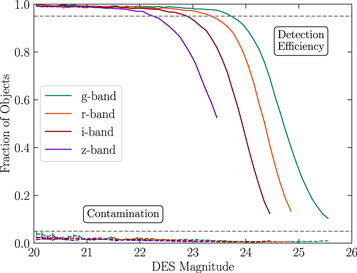
\includegraphics[width=3.12500in]{jira_imgs/404.png}

                \vspace{\dp0}
                } \end{minipage}
        \\ \midrule
    \end{longtable}

\subsection{LVV-T1070 - On-sky Observations: 10-year Depth SV Survey}\label{lvv-t1070}

\begin{longtable}[]{llllll}
\toprule
Version & Status & Priority & Verification Type & Owner
\\\midrule
1 & Draft & Normal &
Demonstration & Keith Bechtol
\\\bottomrule
\multicolumn{6}{c}{ Open \href{https://jira.lsstcorp.org/secure/Tests.jspa\#/testCase/LVV-T1070}{LVV-T1070} in Jira } \\
\end{longtable}

\subsubsection{Verification Elements}
    None.

\subsubsection{Test Items}


\subsubsection{Predecessors}

\subsubsection{Environment Needs}

\paragraph{Software}

\paragraph{Hardware}

\subsubsection{Input Specification}

\subsubsection{Output Specification}

\subsubsection{Test Procedure}
    \begin{longtable}[]{p{1.3cm}p{2cm}p{13cm}}
    %\toprule
    Step & \multicolumn{2}{@{}l}{Description, Input Data and Expected Result} \\ \toprule
    \endhead

            \multirow{3}{*}{ 1 } & Description &
            \begin{minipage}[t]{13cm}{\footnotesize
            
            \vspace{\dp0}
            } \end{minipage} \\ \cline{2-3}
            & Test Data &
            \begin{minipage}[t]{13cm}{\footnotesize
                No data.
                \vspace{\dp0}
            } \end{minipage} \\ \cline{2-3}
            & Expected Result &
        \\ \midrule
    \end{longtable}

\subsection{LVV-T1071 - On-sky Observations: 20-year Depth Test}\label{lvv-t1071}

\begin{longtable}[]{llllll}
\toprule
Version & Status & Priority & Verification Type & Owner
\\\midrule
1 & Draft & Normal &
Demonstration & Keith Bechtol
\\\bottomrule
\multicolumn{6}{c}{ Open \href{https://jira.lsstcorp.org/secure/Tests.jspa\#/testCase/LVV-T1071}{LVV-T1071} in Jira } \\
\end{longtable}

\subsubsection{Verification Elements}
    None.

\subsubsection{Test Items}


\subsubsection{Predecessors}

\subsubsection{Environment Needs}

\paragraph{Software}

\paragraph{Hardware}

\subsubsection{Input Specification}

\subsubsection{Output Specification}

\subsubsection{Test Procedure}
    \begin{longtable}[]{p{1.3cm}p{2cm}p{13cm}}
    %\toprule
    Step & \multicolumn{2}{@{}l}{Description, Input Data and Expected Result} \\ \toprule
    \endhead

            \multirow{3}{*}{ 1 } & Description &
            \begin{minipage}[t]{13cm}{\footnotesize
            
            \vspace{\dp0}
            } \end{minipage} \\ \cline{2-3}
            & Test Data &
            \begin{minipage}[t]{13cm}{\footnotesize
                No data.
                \vspace{\dp0}
            } \end{minipage} \\ \cline{2-3}
            & Expected Result &
        \\ \midrule
    \end{longtable}

\subsection{LVV-T1072 - Data Processing Campaign: Data Release Processing}\label{lvv-t1072}

\begin{longtable}[]{llllll}
\toprule
Version & Status & Priority & Verification Type & Owner
\\\midrule
1 & Draft & Normal &
Demonstration & Keith Bechtol
\\\bottomrule
\multicolumn{6}{c}{ Open \href{https://jira.lsstcorp.org/secure/Tests.jspa\#/testCase/LVV-T1072}{LVV-T1072} in Jira } \\
\end{longtable}

\subsubsection{Verification Elements}
    None.

\subsubsection{Test Items}


\subsubsection{Predecessors}

\subsubsection{Environment Needs}

\paragraph{Software}

\paragraph{Hardware}

\subsubsection{Input Specification}

\subsubsection{Output Specification}

\subsubsection{Test Procedure}
    \begin{longtable}[]{p{1.3cm}p{2cm}p{13cm}}
    %\toprule
    Step & \multicolumn{2}{@{}l}{Description, Input Data and Expected Result} \\ \toprule
    \endhead

            \multirow{3}{*}{ 1 } & Description &
            \begin{minipage}[t]{13cm}{\footnotesize
            
            \vspace{\dp0}
            } \end{minipage} \\ \cline{2-3}
            & Test Data &
            \begin{minipage}[t]{13cm}{\footnotesize
                No data.
                \vspace{\dp0}
            } \end{minipage} \\ \cline{2-3}
            & Expected Result &
        \\ \midrule
    \end{longtable}

\subsection{LVV-T1073 - On-sky Observations: Wide-area SV Survey}\label{lvv-t1073}

\begin{longtable}[]{llllll}
\toprule
Version & Status & Priority & Verification Type & Owner
\\\midrule
1 & Draft & Normal &
Demonstration & Keith Bechtol
\\\bottomrule
\multicolumn{6}{c}{ Open \href{https://jira.lsstcorp.org/secure/Tests.jspa\#/testCase/LVV-T1073}{LVV-T1073} in Jira } \\
\end{longtable}

\subsubsection{Verification Elements}
    None.

\subsubsection{Test Items}


\subsubsection{Predecessors}

\subsubsection{Environment Needs}

\paragraph{Software}

\paragraph{Hardware}

\subsubsection{Input Specification}

\subsubsection{Output Specification}

\subsubsection{Test Procedure}
    \begin{longtable}[]{p{1.3cm}p{2cm}p{13cm}}
    %\toprule
    Step & \multicolumn{2}{@{}l}{Description, Input Data and Expected Result} \\ \toprule
    \endhead

            \multirow{3}{*}{ 1 } & Description &
            \begin{minipage}[t]{13cm}{\footnotesize
            
            \vspace{\dp0}
            } \end{minipage} \\ \cline{2-3}
            & Test Data &
            \begin{minipage}[t]{13cm}{\footnotesize
                No data.
                \vspace{\dp0}
            } \end{minipage} \\ \cline{2-3}
            & Expected Result &
        \\ \midrule
    \end{longtable}

\subsection{LVV-T1074 - Sky Brightness precision}\label{lvv-t1074}

\begin{longtable}[]{llllll}
\toprule
Version & Status & Priority & Verification Type & Owner
\\\midrule
1 & Defined & Normal &
Analysis & Sam Schmidt
\\\bottomrule
\multicolumn{6}{c}{ Open \href{https://jira.lsstcorp.org/secure/Tests.jspa\#/testCase/LVV-T1074}{LVV-T1074} in Jira } \\
\end{longtable}

\subsubsection{Verification Elements}
\begin{itemize}
\item \href{https://jira.lsstcorp.org/browse/LVV-277}{LVV-277} - LSR-REQ-0093-V-05: Photometric Performance5

\item \href{https://jira.lsstcorp.org/browse/LVV-13366}{LVV-13366} - OSS-REQ-0387-V-05: Sky Brightness precision

\end{itemize}

\subsubsection{Test Items}


\subsubsection{Predecessors}

\subsubsection{Environment Needs}

\paragraph{Software}

\paragraph{Hardware}

\subsubsection{Input Specification}

\subsubsection{Output Specification}

\subsubsection{Test Procedure}
    \begin{longtable}[]{p{1.3cm}p{2cm}p{13cm}}
    %\toprule
    Step & \multicolumn{2}{@{}l}{Description, Input Data and Expected Result} \\ \toprule
    \endhead

            \multirow{3}{*}{ 1 } & Description &
            \begin{minipage}[t]{13cm}{\footnotesize
            Select a set of images at a variety of airmasses, Moon, and time to get
a range of sky brightness levels~

            \vspace{\dp0}
            } \end{minipage} \\ \cline{2-3}
            & Test Data &
            \begin{minipage}[t]{13cm}{\footnotesize
                single visit images

                \vspace{\dp0}
            } \end{minipage} \\ \cline{2-3}
            & Expected Result &
        \\ \midrule

            \multirow{3}{*}{ 2 } & Description &
            \begin{minipage}[t]{13cm}{\footnotesize
            Run DM Stack, part of which will generate polynomial fit to sky
brightness

            \vspace{\dp0}
            } \end{minipage} \\ \cline{2-3}
            & Test Data &
            \begin{minipage}[t]{13cm}{\footnotesize
                images from step 1

                \vspace{\dp0}
            } \end{minipage} \\ \cline{2-3}
            & Expected Result &
                \begin{minipage}[t]{13cm}{\footnotesize
                polynomial fit of sky brightness

                \vspace{\dp0}
                } \end{minipage}
        \\ \midrule

            \multirow{3}{*}{ 3 } & Description &
            \begin{minipage}[t]{13cm}{\footnotesize
            Compare sky brightness estimate from the polynomial fit to measures of
the sky brightness at specific points, test whether these agree to
SBPrec{[}1 percent{]}

            \vspace{\dp0}
            } \end{minipage} \\ \cline{2-3}
            & Test Data &
            \begin{minipage}[t]{13cm}{\footnotesize
                polynomial fit from step 2

                \vspace{\dp0}
            } \end{minipage} \\ \cline{2-3}
            & Expected Result &
                \begin{minipage}[t]{13cm}{\footnotesize
                pass fail for SBPrec test

                \vspace{\dp0}
                } \end{minipage}
        \\ \midrule
    \end{longtable}

\subsection{LVV-T1075 - Sky Brightness Precision 2 (Simulated Data)}\label{lvv-t1075}

\begin{longtable}[]{llllll}
\toprule
Version & Status & Priority & Verification Type & Owner
\\\midrule
1 & Defined & Normal &
Analysis & Sam Schmidt
\\\bottomrule
\multicolumn{6}{c}{ Open \href{https://jira.lsstcorp.org/secure/Tests.jspa\#/testCase/LVV-T1075}{LVV-T1075} in Jira } \\
\end{longtable}

\subsubsection{Verification Elements}
\begin{itemize}
\item \href{https://jira.lsstcorp.org/browse/LVV-277}{LVV-277} - LSR-REQ-0093-V-05: Photometric Performance5

\item \href{https://jira.lsstcorp.org/browse/LVV-13366}{LVV-13366} - OSS-REQ-0387-V-05: Sky Brightness precision

\end{itemize}

\subsubsection{Test Items}


\subsubsection{Predecessors}

\subsubsection{Environment Needs}

\paragraph{Software}

\paragraph{Hardware}

\subsubsection{Input Specification}

\subsubsection{Output Specification}

\subsubsection{Test Procedure}
    \begin{longtable}[]{p{1.3cm}p{2cm}p{13cm}}
    %\toprule
    Step & \multicolumn{2}{@{}l}{Description, Input Data and Expected Result} \\ \toprule
    \endhead

            \multirow{3}{*}{ 1 } & Description &
            \begin{minipage}[t]{13cm}{\footnotesize
            Generate simulated images with a known sky brightness, simulate
conditions with a range of airmass, Moon, atmosphere to get a range of
brightness conditions

            \vspace{\dp0}
            } \end{minipage} \\ \cline{2-3}
            & Test Data &
            \begin{minipage}[t]{13cm}{\footnotesize
                New simulated image data

                \vspace{\dp0}
            } \end{minipage} \\ \cline{2-3}
            & Expected Result &
        \\ \midrule

            \multirow{3}{*}{ 2 } & Description &
            \begin{minipage}[t]{13cm}{\footnotesize
            Run DM Stack processing, which generates polynomial fit to the sky
brightness

            \vspace{\dp0}
            } \end{minipage} \\ \cline{2-3}
            & Test Data &
            \begin{minipage}[t]{13cm}{\footnotesize
                images from step 1

                \vspace{\dp0}
            } \end{minipage} \\ \cline{2-3}
            & Expected Result &
                \begin{minipage}[t]{13cm}{\footnotesize
                sky brightness model

                \vspace{\dp0}
                } \end{minipage}
        \\ \midrule

            \multirow{3}{*}{ 3 } & Description &
            \begin{minipage}[t]{13cm}{\footnotesize
            Compare sky brightness to truth evaluated at points not used in the
polynomial grid determination, check that these agree to within SBPrec
{[}1 percent{]}

            \vspace{\dp0}
            } \end{minipage} \\ \cline{2-3}
            & Test Data &
            \begin{minipage}[t]{13cm}{\footnotesize
                brightness model

                \vspace{\dp0}
            } \end{minipage} \\ \cline{2-3}
            & Expected Result &
                \begin{minipage}[t]{13cm}{\footnotesize
                pass/fail for SBPrec test

                \vspace{\dp0}
                } \end{minipage}
        \\ \midrule
    \end{longtable}

\subsection{LVV-T1078 - Generate matched DIASource catalog}\label{lvv-t1078}

\begin{longtable}[]{llllll}
\toprule
Version & Status & Priority & Verification Type & Owner
\\\midrule
1 & Draft & Normal &
Test & Bryce Kalmbach
\\\bottomrule
\multicolumn{6}{c}{ Open \href{https://jira.lsstcorp.org/secure/Tests.jspa\#/testCase/LVV-T1078}{LVV-T1078} in Jira } \\
\end{longtable}

\subsubsection{Verification Elements}
    None.

\subsubsection{Test Items}


\subsubsection{Predecessors}

\subsubsection{Environment Needs}

\paragraph{Software}

\paragraph{Hardware}

\subsubsection{Input Specification}

\subsubsection{Output Specification}

\subsubsection{Test Procedure}
    \begin{longtable}[]{p{1.3cm}p{2cm}p{13cm}}
    %\toprule
    Step & \multicolumn{2}{@{}l}{Description, Input Data and Expected Result} \\ \toprule
    \endhead

            \multirow{3}{*}{ 1 } & Description &
            \begin{minipage}[t]{13cm}{\footnotesize
            Generate catalog of simulated variable/transient sources

\begin{itemize}
\tightlist
\item
  Sources should have the ~distribution of brightnesses expected for the
  LSST to 1 magnitude below the single visit detection limit
\item
  Sources will be assumed as point sources
\item
  Sources will include their light curve in all LSST passbands
\end{itemize}

            \vspace{\dp0}
            } \end{minipage} \\ \cline{2-3}
            & Test Data &
            \begin{minipage}[t]{13cm}{\footnotesize
                No data.
                \vspace{\dp0}
            } \end{minipage} \\ \cline{2-3}
            & Expected Result &
        \\ \midrule

            \multirow{3}{*}{ 2 } & Description &
            \begin{minipage}[t]{13cm}{\footnotesize
            Inject simulated variables/transients into single visit images (after
ISR) images. Images will be selected to be \textgreater{}30 degrees from
the Ecliptic to avoid moving source contamination

            \vspace{\dp0}
            } \end{minipage} \\ \cline{2-3}
            & Test Data &
            \begin{minipage}[t]{13cm}{\footnotesize
                Real Images

                \vspace{\dp0}
            } \end{minipage} \\ \cline{2-3}
            & Expected Result &
        \\ \midrule

            \multirow{3}{*}{ 3 } & Description &
            \begin{minipage}[t]{13cm}{\footnotesize
            Run difference imaging on images with injected variables/transients.
Including output from spuriousness classification algorithm

            \vspace{\dp0}
            } \end{minipage} \\ \cline{2-3}
            & Test Data &
            \begin{minipage}[t]{13cm}{\footnotesize
                Images from Step 2

                \vspace{\dp0}
            } \end{minipage} \\ \cline{2-3}
            & Expected Result &
        \\ \midrule

            \multirow{3}{*}{ 4 } & Description &
            \begin{minipage}[t]{13cm}{\footnotesize
            Match the input catalog and the DIASource lists

            \vspace{\dp0}
            } \end{minipage} \\ \cline{2-3}
            & Test Data &
            \begin{minipage}[t]{13cm}{\footnotesize
                No data.
                \vspace{\dp0}
            } \end{minipage} \\ \cline{2-3}
            & Expected Result &
        \\ \midrule
    \end{longtable}

\subsection{LVV-T1081 - Completeness vs. magnitude via external catalogs}\label{lvv-t1081}

\begin{longtable}[]{llllll}
\toprule
Version & Status & Priority & Verification Type & Owner
\\\midrule
1 & Defined & Normal &
Test & Jeffrey Carlin
\\\bottomrule
\multicolumn{6}{c}{ Open \href{https://jira.lsstcorp.org/secure/Tests.jspa\#/testCase/LVV-T1081}{LVV-T1081} in Jira } \\
\end{longtable}

\subsubsection{Verification Elements}
\begin{itemize}
\item \href{https://jira.lsstcorp.org/browse/LVV-1315}{LVV-1315} - OSS-REQ-0164-V-01: Catalog Completeness and Reliability

\end{itemize}

\subsubsection{Test Items}
Estimate completeness vs. magnitude for stars and galaxies by comparison
to an external ``truth'' catalog. Note that in practice there are no
external catalogs deep enough to separate stars from galaxies over the
relevant magnitude range, so that this comparison will likely measure
detection completeness of all sources from the external catalog.


\subsubsection{Predecessors}
\href{https://jira.lsstcorp.org/secure/Tests.jspa\#/testCase/LVV-T1070}{LVV-T1070}
or
​\href{https://jira.lsstcorp.org/secure/Tests.jspa\#/testCase/LVV-T1071}{LVV-T1071}​​​

\subsubsection{Environment Needs}

\paragraph{Software}

\paragraph{Hardware}

\subsubsection{Input Specification}
This test requires a dataset observed by LSST that overlaps an external
catalog with space-based (i.e., high spatial resolution) observations
enabling high quality source classification. (For example, the HST
COSMOS data.) It is likely that no catalog exists that is as deep as
LSST 10-year survey data, so a magnitude limit may have to be applied to
the catalogs when comparing.

\subsubsection{Output Specification}

\subsubsection{Test Procedure}
    \begin{longtable}[]{p{1.3cm}p{2cm}p{13cm}}
    %\toprule
    Step & \multicolumn{2}{@{}l}{Description, Input Data and Expected Result} \\ \toprule
    \endhead

            \multirow{3}{*}{ 1 } & Description &
            \begin{minipage}[t]{13cm}{\footnotesize
            Point the butler to appropriate overlapping data sets.

            \vspace{\dp0}
            } \end{minipage} \\ \cline{2-3}
            & Test Data &
            \begin{minipage}[t]{13cm}{\footnotesize
                No data.
                \vspace{\dp0}
            } \end{minipage} \\ \cline{2-3}
            & Expected Result &
        \\ \midrule

            \multirow{3}{*}{ 2 } & Description &
            \begin{minipage}[t]{13cm}{\footnotesize
            Point the butler to the appropriate deep LSST catalog.

            \vspace{\dp0}
            } \end{minipage} \\ \cline{2-3}
            & Test Data &
            \begin{minipage}[t]{13cm}{\footnotesize
                No data.
                \vspace{\dp0}
            } \end{minipage} \\ \cline{2-3}
            & Expected Result &
        \\ \midrule

            \multirow{3}{*}{ 3 } & Description &
            \begin{minipage}[t]{13cm}{\footnotesize
            For each object in the external reference catalog, check if there is a
corresponding detected object in the LSST catalog.\\[2\baselineskip]The
matching should be done via position, but may be improved by requiring
similar magnitudes between the two catalogs (keeping in mind that
variable, yet persistent, objects may present different brightness, and
thus would not necessarily pass a magnitude criterion).

            \vspace{\dp0}
            } \end{minipage} \\ \cline{2-3}
            & Test Data &
            \begin{minipage}[t]{13cm}{\footnotesize
                No data.
                \vspace{\dp0}
            } \end{minipage} \\ \cline{2-3}
            & Expected Result &
        \\ \midrule

            \multirow{3}{*}{ 4 } & Description &
            \begin{minipage}[t]{13cm}{\footnotesize
            In magnitude bins, count the fraction of objects from the external
catalog that had a corresponding object in the LSST dataset. Plot this
fraction (the ``completeness'') as a function of magnitude.

            \vspace{\dp0}
            } \end{minipage} \\ \cline{2-3}
            & Test Data &
            \begin{minipage}[t]{13cm}{\footnotesize
                No data.
                \vspace{\dp0}
            } \end{minipage} \\ \cline{2-3}
            & Expected Result &
                \begin{minipage}[t]{13cm}{\footnotesize
                A figure similar to Fig. 15 of the
\href{https://arxiv.org/pdf/1702.08449.pdf}{HSC DR1 paper}.

                \vspace{\dp0}
                } \end{minipage}
        \\ \midrule
    \end{longtable}

\subsection{LVV-T1082 - Completeness vs. magnitude via injected sources}\label{lvv-t1082}

\begin{longtable}[]{llllll}
\toprule
Version & Status & Priority & Verification Type & Owner
\\\midrule
1 & Defined & Normal &
Test & Jeffrey Carlin
\\\bottomrule
\multicolumn{6}{c}{ Open \href{https://jira.lsstcorp.org/secure/Tests.jspa\#/testCase/LVV-T1082}{LVV-T1082} in Jira } \\
\end{longtable}

\subsubsection{Verification Elements}
\begin{itemize}
\item \href{https://jira.lsstcorp.org/browse/LVV-1315}{LVV-1315} - OSS-REQ-0164-V-01: Catalog Completeness and Reliability

\end{itemize}

\subsubsection{Test Items}
Estimate completeness vs. magnitude for stars and galaxies by inserting
artificial sources into observed LSST data.


\subsubsection{Predecessors}
\href{https://jira.lsstcorp.org/secure/Tests.jspa\#/testCase/LVV-T1070}{LVV-T1070}
or
​\href{https://jira.lsstcorp.org/secure/Tests.jspa\#/testCase/LVV-T1071}{LVV-T1071}​​​

\subsubsection{Environment Needs}

\paragraph{Software}

\paragraph{Hardware}

\subsubsection{Input Specification}

\subsubsection{Output Specification}

\subsubsection{Test Procedure}
    \begin{longtable}[]{p{1.3cm}p{2cm}p{13cm}}
    %\toprule
    Step & \multicolumn{2}{@{}l}{Description, Input Data and Expected Result} \\ \toprule
    \endhead

            \multirow{3}{*}{ 1 } & Description &
            \begin{minipage}[t]{13cm}{\footnotesize
            Identify several tracts in the observed data, spanning a range of
Galactic latitudes/source densities.~

            \vspace{\dp0}
            } \end{minipage} \\ \cline{2-3}
            & Test Data &
            \begin{minipage}[t]{13cm}{\footnotesize
                No data.
                \vspace{\dp0}
            } \end{minipage} \\ \cline{2-3}
            & Expected Result &
        \\ \midrule

            \multirow{3}{*}{ 2 } & Description &
            \begin{minipage}[t]{13cm}{\footnotesize
            Create catalogs of artificial sources to be inserted into the images. To
ensure statistically robust results, at least 1000 objects per magnitude
bin should be included.

            \vspace{\dp0}
            } \end{minipage} \\ \cline{2-3}
            & Test Data &
            \begin{minipage}[t]{13cm}{\footnotesize
                The artificial star catalog should span the range of colors typical of
Milky Way stars, and the expected magnitudes to which the input data are
sensitive (e.g., the GalFast simulated catalog). Artificial galaxies
should be drawn from a synthetic catalog (e.g., the DESC Data Challenge
galaxy catalogs).

                \vspace{\dp0}
            } \end{minipage} \\ \cline{2-3}
            & Expected Result &
        \\ \midrule

            \multirow{3}{*}{ 3 } & Description &
            \begin{minipage}[t]{13cm}{\footnotesize
            Identify the images into which you will insert sources, and run the fake
source code (in the current LSST Stack, the `Synpipe' routine(s)).
Ideally these should be injected into the individual visit images, but
if that is computationally prohibitive, inserting them into coadds would
be acceptable.

            \vspace{\dp0}
            } \end{minipage} \\ \cline{2-3}
            & Test Data &
            \begin{minipage}[t]{13cm}{\footnotesize
                No data.
                \vspace{\dp0}
            } \end{minipage} \\ \cline{2-3}
            & Expected Result &
        \\ \midrule

            \multirow{3}{*}{ 4 } & Description &
            \begin{minipage}[t]{13cm}{\footnotesize
            Run the source detection and measurement algorithms on the images
resulting from the previous steps.

            \vspace{\dp0}
            } \end{minipage} \\ \cline{2-3}
            & Test Data &
            \begin{minipage}[t]{13cm}{\footnotesize
                No data.
                \vspace{\dp0}
            } \end{minipage} \\ \cline{2-3}
            & Expected Result &
        \\ \midrule

            \multirow{3}{*}{ 5 } & Description &
            \begin{minipage}[t]{13cm}{\footnotesize
            Point the Butler to the catalog resulting from the previous step.

            \vspace{\dp0}
            } \end{minipage} \\ \cline{2-3}
            & Test Data &
            \begin{minipage}[t]{13cm}{\footnotesize
                No data.
                \vspace{\dp0}
            } \end{minipage} \\ \cline{2-3}
            & Expected Result &
        \\ \midrule

            \multirow{3}{*}{ 6 } & Description &
            \begin{minipage}[t]{13cm}{\footnotesize
            Define the criteria for matching of sources. Because the positions of
injected sources are known, a small matching radius can be used.

            \vspace{\dp0}
            } \end{minipage} \\ \cline{2-3}
            & Test Data &
            \begin{minipage}[t]{13cm}{\footnotesize
                No data.
                \vspace{\dp0}
            } \end{minipage} \\ \cline{2-3}
            & Expected Result &
        \\ \midrule

            \multirow{3}{*}{ 7 } & Description &
            \begin{minipage}[t]{13cm}{\footnotesize
            For each object in the input artificial source catalog, check if there
is a corresponding detected object in the output LSST
catalog.\\[2\baselineskip]The matching should be done via position, but
may be improved by requiring similar magnitudes between the two
catalogs.

            \vspace{\dp0}
            } \end{minipage} \\ \cline{2-3}
            & Test Data &
            \begin{minipage}[t]{13cm}{\footnotesize
                No data.
                \vspace{\dp0}
            } \end{minipage} \\ \cline{2-3}
            & Expected Result &
        \\ \midrule

            \multirow{3}{*}{ 8 } & Description &
            \begin{minipage}[t]{13cm}{\footnotesize
            In magnitude bins, count the fraction of objects from the input
``truth'' catalog that had a corresponding detected object in the LSST
dataset. Plot this fraction (the ``completeness'') as a function of
magnitude, for (1) all sources, (2) objects inserted as stars, and (3)
objects inserted as galaxies.

            \vspace{\dp0}
            } \end{minipage} \\ \cline{2-3}
            & Test Data &
            \begin{minipage}[t]{13cm}{\footnotesize
                No data.
                \vspace{\dp0}
            } \end{minipage} \\ \cline{2-3}
            & Expected Result &
                \begin{minipage}[t]{13cm}{\footnotesize
                A figure similar to Fig. 15 of the
\href{https://arxiv.org/pdf/1702.08449.pdf}{HSC DR1 paper}, but with
separate curves for stars and galaxies.

                \vspace{\dp0}
                } \end{minipage}
        \\ \midrule
    \end{longtable}

\subsection{LVV-T1083 - Single Visit Ellipticity Residuals w/ on sky data}\label{lvv-t1083}

\begin{longtable}[]{llllll}
\toprule
Version & Status & Priority & Verification Type & Owner
\\\midrule
1 & Defined & Normal &
Analysis & Imram Hasan
\\\bottomrule
\multicolumn{6}{c}{ Open \href{https://jira.lsstcorp.org/secure/Tests.jspa\#/testCase/LVV-T1083}{LVV-T1083} in Jira } \\
\end{longtable}

\subsubsection{Verification Elements}
\begin{itemize}
\item \href{https://jira.lsstcorp.org/browse/LVV-1366}{LVV-1366} - OSS-REQ-0390-V-01: Ellipticity Correlations

\end{itemize}

\subsubsection{Test Items}
Confirm the amplitude of elipticity residual correlations is within spec


\subsubsection{Predecessors}
\href{https://jira.lsstcorp.org/secure/Tests.jspa\#/testCase/LVV-T1070}{LVV-T1070}
or
​\href{https://jira.lsstcorp.org/secure/Tests.jspa\#/testCase/LVV-T1071}{LVV-T1071}​​​

\subsubsection{Environment Needs}

\paragraph{Software}

\paragraph{Hardware}

\subsubsection{Input Specification}

\subsubsection{Output Specification}

\subsubsection{Test Procedure}
    \begin{longtable}[]{p{1.3cm}p{2cm}p{13cm}}
    %\toprule
    Step & \multicolumn{2}{@{}l}{Description, Input Data and Expected Result} \\ \toprule
    \endhead

            \multirow{3}{*}{ 1 } & Description &
            \begin{minipage}[t]{13cm}{\footnotesize
            Point the butler at the single visit comissioning data. We will need the
individual PSF models and the calexp catalogs

            \vspace{\dp0}
            } \end{minipage} \\ \cline{2-3}
            & Test Data &
            \begin{minipage}[t]{13cm}{\footnotesize
                No data.
                \vspace{\dp0}
            } \end{minipage} \\ \cline{2-3}
            & Expected Result &
        \\ \midrule

            \multirow{3}{*}{ 2 } & Description &
            \begin{minipage}[t]{13cm}{\footnotesize
            Obtain calexps src catalogs that are well representative of observing
conditions, eg cover a range of airmasses, seeing conditions, moon
brightness etc.\\[2\baselineskip]obtain the PSF models from these
calexps as well.

            \vspace{\dp0}
            } \end{minipage} \\ \cline{2-3}
            & Test Data &
            \begin{minipage}[t]{13cm}{\footnotesize
                No data.
                \vspace{\dp0}
            } \end{minipage} \\ \cline{2-3}
            & Expected Result &
        \\ \midrule

            \multirow{3}{*}{ 3 } & Description &
            \begin{minipage}[t]{13cm}{\footnotesize
            Consider separately stars that were included in PSF modeling and stars
that were not included in PSF modeling. The fiduciual result for this
test should use the stars that were not included in PSF modeling. The
stars that were included in PSF modeling will still be useful for
diagnostic purposes.

            \vspace{\dp0}
            } \end{minipage} \\ \cline{2-3}
            & Test Data &
            \begin{minipage}[t]{13cm}{\footnotesize
                No data.
                \vspace{\dp0}
            } \end{minipage} \\ \cline{2-3}
            & Expected Result &
        \\ \midrule

            \multirow{3}{*}{ 4 } & Description &
            \begin{minipage}[t]{13cm}{\footnotesize
            For each stellar sample, compute all Rowe statistics over angular scales
ranging from less than 1 arcmin to greater than 5
arcmin.\\[2\baselineskip]This will require the PSF model for calculating
residuals. To calculate residuals, obtain the PSF model evaluated at the
positions of stars of interest, and find the difference in the measured
ellipticity of stars, and the model ellipticity.

            \vspace{\dp0}
            } \end{minipage} \\ \cline{2-3}
            & Test Data &
            \begin{minipage}[t]{13cm}{\footnotesize
                No data.
                \vspace{\dp0}
            } \end{minipage} \\ \cline{2-3}
            & Expected Result &
        \\ \midrule

            \multirow{3}{*}{ 5 } & Description &
            \begin{minipage}[t]{13cm}{\footnotesize
            Extract the amplitudes of the Rowe statistics at angular scales of 1
arcmin and less, and 5 arcmin and larger

            \vspace{\dp0}
            } \end{minipage} \\ \cline{2-3}
            & Test Data &
            \begin{minipage}[t]{13cm}{\footnotesize
                No data.
                \vspace{\dp0}
            } \end{minipage} \\ \cline{2-3}
            & Expected Result &
        \\ \midrule

            \multirow{3}{*}{ 6 } & Description &
            \begin{minipage}[t]{13cm}{\footnotesize
            For each angular scale (\textless{}1 arcmin and \textgreater{}5 arcmin),
for each Rowe statistic, collect the amplitudes of the Rho statistics.

            \vspace{\dp0}
            } \end{minipage} \\ \cline{2-3}
            & Test Data &
            \begin{minipage}[t]{13cm}{\footnotesize
                No data.
                \vspace{\dp0}
            } \end{minipage} \\ \cline{2-3}
            & Expected Result &
        \\ \midrule

            \multirow{3}{*}{ 7 } & Description &
            \begin{minipage}[t]{13cm}{\footnotesize
            Calculate the medians from the amplitudes corresponding to each angular
scale, for each Rowe statistic.

            \vspace{\dp0}
            } \end{minipage} \\ \cline{2-3}
            & Test Data &
            \begin{minipage}[t]{13cm}{\footnotesize
                No data.
                \vspace{\dp0}
            } \end{minipage} \\ \cline{2-3}
            & Expected Result &
        \\ \midrule

            \multirow{3}{*}{ 8 } & Description &
            \begin{minipage}[t]{13cm}{\footnotesize
            Calculate the fraction of exposures where the medians of amplitudes are
within the specifications for individual calexp exposures, and outside
of specifications for the \textless{}1 arcsec and \textgreater{}5 arcsec
scales

            \vspace{\dp0}
            } \end{minipage} \\ \cline{2-3}
            & Test Data &
            \begin{minipage}[t]{13cm}{\footnotesize
                No data.
                \vspace{\dp0}
            } \end{minipage} \\ \cline{2-3}
            & Expected Result &
        \\ \midrule

            \multirow{3}{*}{ 9 } & Description &
            \begin{minipage}[t]{13cm}{\footnotesize
            Confirm that the fraction of single visit Rowe Statistics outside of
spec is less than 15\% (TEF)

            \vspace{\dp0}
            } \end{minipage} \\ \cline{2-3}
            & Test Data &
            \begin{minipage}[t]{13cm}{\footnotesize
                No data.
                \vspace{\dp0}
            } \end{minipage} \\ \cline{2-3}
            & Expected Result &
        \\ \midrule
    \end{longtable}

\subsection{LVV-T1084 - Smoothness of Rowe statistics on angular scales of 1 arcmin \textless{}
theta \textless{} 5 arcmin}\label{lvv-t1084}

\begin{longtable}[]{llllll}
\toprule
Version & Status & Priority & Verification Type & Owner
\\\midrule
1 & Defined & Normal &
Analysis & Imram Hasan
\\\bottomrule
\multicolumn{6}{c}{ Open \href{https://jira.lsstcorp.org/secure/Tests.jspa\#/testCase/LVV-T1084}{LVV-T1084} in Jira } \\
\end{longtable}

\subsubsection{Verification Elements}
\begin{itemize}
\item \href{https://jira.lsstcorp.org/browse/LVV-1366}{LVV-1366} - OSS-REQ-0390-V-01: Ellipticity Correlations

\end{itemize}

\subsubsection{Test Items}


\subsubsection{Predecessors}
\href{https://jira.lsstcorp.org/secure/Tests.jspa\#/testCase/LVV-T361}{LVV-T361
(1.0)}

\subsubsection{Environment Needs}

\paragraph{Software}

\paragraph{Hardware}

\subsubsection{Input Specification}

\subsubsection{Output Specification}

\subsubsection{Test Procedure}
    \begin{longtable}[]{p{1.3cm}p{2cm}p{13cm}}
    %\toprule
    Step & \multicolumn{2}{@{}l}{Description, Input Data and Expected Result} \\ \toprule
    \endhead

            \multirow{3}{*}{ 1 } & Description &
            \begin{minipage}[t]{13cm}{\footnotesize
            Get the final Rowe statistics that were calculated in test case
\href{https://jira.lsstcorp.org/secure/Tests.jspa\#/testCase/LVV-T361}{LVV-T361
(1.0)}in step 4

            \vspace{\dp0}
            } \end{minipage} \\ \cline{2-3}
            & Test Data &
            \begin{minipage}[t]{13cm}{\footnotesize
                No data.
                \vspace{\dp0}
            } \end{minipage} \\ \cline{2-3}
            & Expected Result &
        \\ \midrule

            \multirow{3}{*}{ 2 } & Description &
            \begin{minipage}[t]{13cm}{\footnotesize
            For all Rowe statistics, examine by eye the amplitudes between the
angular scales of 1 arcmin \textless{} theta \textless{} 5 arcmin

            \vspace{\dp0}
            } \end{minipage} \\ \cline{2-3}
            & Test Data &
            \begin{minipage}[t]{13cm}{\footnotesize
                No data.
                \vspace{\dp0}
            } \end{minipage} \\ \cline{2-3}
            & Expected Result &
        \\ \midrule

            \multirow{3}{*}{ 3 } & Description &
            \begin{minipage}[t]{13cm}{\footnotesize
            Confirm that the amplitudes vary smoothly between these angular scales

            \vspace{\dp0}
            } \end{minipage} \\ \cline{2-3}
            & Test Data &
            \begin{minipage}[t]{13cm}{\footnotesize
                No data.
                \vspace{\dp0}
            } \end{minipage} \\ \cline{2-3}
            & Expected Result &
        \\ \midrule
    \end{longtable}

\subsection{LVV-T1278 - Relative Astrometric Performance (Repeatability)}\label{lvv-t1278}

\begin{longtable}[]{llllll}
\toprule
Version & Status & Priority & Verification Type & Owner
\\\midrule
1 & Defined & Normal &
Test & Bryce Kalmbach
\\\bottomrule
\multicolumn{6}{c}{ Open \href{https://jira.lsstcorp.org/secure/Tests.jspa\#/testCase/LVV-T1278}{LVV-T1278} in Jira } \\
\end{longtable}

\subsubsection{Verification Elements}
\begin{itemize}
\item \href{https://jira.lsstcorp.org/browse/LVV-1363}{LVV-1363} - OSS-REQ-0388-V-01: Astrometric Performance

\end{itemize}

\subsubsection{Test Items}
Verify that relative astrometric separations are as accurate as
specified


\subsubsection{Predecessors}

\subsubsection{Environment Needs}

\paragraph{Software}

\paragraph{Hardware}

\subsubsection{Input Specification}

\subsubsection{Output Specification}

\subsubsection{Test Procedure}
    \begin{longtable}[]{p{1.3cm}p{2cm}p{13cm}}
    %\toprule
    Step & \multicolumn{2}{@{}l}{Description, Input Data and Expected Result} \\ \toprule
    \endhead

            \multirow{3}{*}{ 1 } & Description &
            \begin{minipage}[t]{13cm}{\footnotesize
            Image an average field. Repeat at different airmasses.

            \vspace{\dp0}
            } \end{minipage} \\ \cline{2-3}
            & Test Data &
            \begin{minipage}[t]{13cm}{\footnotesize
                No data.
                \vspace{\dp0}
            } \end{minipage} \\ \cline{2-3}
            & Expected Result &
        \\ \midrule

            \multirow{3}{*}{ 2 } & Description &
            \begin{minipage}[t]{13cm}{\footnotesize
            Run source detection and astrometric measurement on images from step 1

            \vspace{\dp0}
            } \end{minipage} \\ \cline{2-3}
            & Test Data &
            \begin{minipage}[t]{13cm}{\footnotesize
                Images from Step 1

                \vspace{\dp0}
            } \end{minipage} \\ \cline{2-3}
            & Expected Result &
        \\ \midrule

            \multirow{3}{*}{ 3 } & Description &
            \begin{minipage}[t]{13cm}{\footnotesize
            Calculate the separations between all sources detected in step 2

            \vspace{\dp0}
            } \end{minipage} \\ \cline{2-3}
            & Test Data &
            \begin{minipage}[t]{13cm}{\footnotesize
                Matched source catalogs from Step 2

                \vspace{\dp0}
            } \end{minipage} \\ \cline{2-3}
            & Expected Result &
        \\ \midrule

            \multirow{3}{*}{ 4 } & Description &
            \begin{minipage}[t]{13cm}{\footnotesize
            Compare source separations from step 3. Calculate RMS for each pair
across set of visits.

            \vspace{\dp0}
            } \end{minipage} \\ \cline{2-3}
            & Test Data &
            \begin{minipage}[t]{13cm}{\footnotesize
                Source separations from Step 3.

                \vspace{\dp0}
            } \end{minipage} \\ \cline{2-3}
            & Expected Result &
        \\ \midrule

            \multirow{3}{*}{ 5 } & Description &
            \begin{minipage}[t]{13cm}{\footnotesize
            Examine distribution of source separation RMS from step 4 for all pairs
of sources separated by \textasciitilde{} 5 arcminutes. Verify that the
median in these measurements is \textless{}= 10 milliarcseconds

            \vspace{\dp0}
            } \end{minipage} \\ \cline{2-3}
            & Test Data &
            \begin{minipage}[t]{13cm}{\footnotesize
                Source separations form Step 4. Positions from Matched Source catalogs
from Step 2.

                \vspace{\dp0}
            } \end{minipage} \\ \cline{2-3}
            & Expected Result &
        \\ \midrule

            \multirow{3}{*}{ 6 } & Description &
            \begin{minipage}[t]{13cm}{\footnotesize
            Verify that no more than 10\% of the source pairs separated by
\textasciitilde{} 5 arcminutes have separation RMS greater than 20
milliarcseconds

            \vspace{\dp0}
            } \end{minipage} \\ \cline{2-3}
            & Test Data &
            \begin{minipage}[t]{13cm}{\footnotesize
                Source separations form Step 4. Positions from Matched Source catalogs
from Step 2.

                \vspace{\dp0}
            } \end{minipage} \\ \cline{2-3}
            & Expected Result &
        \\ \midrule

            \multirow{3}{*}{ 7 } & Description &
            \begin{minipage}[t]{13cm}{\footnotesize
            Examine distribution of source separation RMS from step 4 for all pairs
of sources separated by \textasciitilde{} 20 arcminutes. Verify that the
median in these measurements is \textless{}= 10 milliarcseconds

            \vspace{\dp0}
            } \end{minipage} \\ \cline{2-3}
            & Test Data &
            \begin{minipage}[t]{13cm}{\footnotesize
                Source separations form Step 4. Positions from Matched Source catalogs
from Step 2.

                \vspace{\dp0}
            } \end{minipage} \\ \cline{2-3}
            & Expected Result &
        \\ \midrule

            \multirow{3}{*}{ 8 } & Description &
            \begin{minipage}[t]{13cm}{\footnotesize
            Verify that no more than 10\% of the source pairs separated by
\textasciitilde{} 20 arcminutes have separation RMS greater than 20
milliarcseconds

            \vspace{\dp0}
            } \end{minipage} \\ \cline{2-3}
            & Test Data &
            \begin{minipage}[t]{13cm}{\footnotesize
                Source separations form Step 4. Positions from Matched Source catalogs
from Step 2.

                \vspace{\dp0}
            } \end{minipage} \\ \cline{2-3}
            & Expected Result &
        \\ \midrule

            \multirow{3}{*}{ 9 } & Description &
            \begin{minipage}[t]{13cm}{\footnotesize
            Examine distribution of source separation RMS from step 4 for all pairs
of sources separated by \textasciitilde{} 200 arcminutes. Verify that
the median in these measurements is \textless{}= 15 milliarcseconds

            \vspace{\dp0}
            } \end{minipage} \\ \cline{2-3}
            & Test Data &
            \begin{minipage}[t]{13cm}{\footnotesize
                Source separations form Step 4. Positions from Matched Source catalogs
from Step 2.

                \vspace{\dp0}
            } \end{minipage} \\ \cline{2-3}
            & Expected Result &
        \\ \midrule

            \multirow{3}{*}{ 10 } & Description &
            \begin{minipage}[t]{13cm}{\footnotesize
            Verify that no more than 10\% of the source pairs separated by
\textasciitilde{} 200 arcminutes have separation RMS greater than 30
milliarcseconds

            \vspace{\dp0}
            } \end{minipage} \\ \cline{2-3}
            & Test Data &
            \begin{minipage}[t]{13cm}{\footnotesize
                Source separations form Step 4. Positions from Matched Source catalogs
from Step 2.

                \vspace{\dp0}
            } \end{minipage} \\ \cline{2-3}
            & Expected Result &
        \\ \midrule
    \end{longtable}

\newpage
\section{Reusable Test Cases}

Test cases in this section are made up of commonly encountered steps that have been factored out into modular, reusable scripts.
These test cases are meant solely for the building of actual tests used for verification, to be inserted in test scripts via the “Call to Test” functionality in Jira/ATM.
They streamline the process of writing test scripts by providing pre-designed steps, while also ensuring homogeneity throughout the test suite.
These reusable modules are not themselves verifying requirements.
Also, these test cases shall not call other reusable test cases in their script.




\subsection{LVV-T33 - Verify implementation of Raw Science Image Metadata}\label{lvv-t33}

\begin{longtable}[]{llllll}
\toprule
Version & Status & Priority & Verification Type & Owner
\\\midrule
1 & Defined & Normal &
Test & Kian-Tat Lim
\\\bottomrule
\multicolumn{6}{c}{ Open \href{https://jira.lsstcorp.org/secure/Tests.jspa\#/testCase/LVV-T33}{LVV-T33} in Jira } \\
\end{longtable}

\subsubsection{Test Items}
Verify successful ingestion of raw data from L1 Test Stand DAQ and that
image metadata is present and queryable.


\subsubsection{Predecessors}
\href{https://jira.lsstcorp.org/secure/Tests.jspa\#/testCase/LVV-T29}{LVV-T29},
​\href{https://jira.lsstcorp.org/secure/Tests.jspa\#/testCase/LVV-T32}{LVV-T32}​​​






\subsubsection{Test Procedure}
    \begin{longtable}[]{p{1.3cm}p{2cm}p{13cm}}
    %\toprule
    Step & \multicolumn{2}{@{}l}{Description, Input Data and Expected Result} \\ \toprule
    \endhead
            \multirow{3}{*}{\parbox{1.3cm}{ 1
} }
& {\small Description} &
\begin{minipage}[t]{13cm}{\scriptsize
Identify (or gather) a dataset of raw science images.

\vspace{\dp0}
} \end{minipage} \\ \cdashline{2-3}
& {\small Test Data} &
\\ \cdashline{2-3}
& {\small Expected Result} &
\\ \hdashline
        \\ \midrule
            \multirow{3}{*}{\parbox{1.3cm}{ 2
} }
& {\small Description} &
\begin{minipage}[t]{13cm}{\scriptsize
Verify that time of exposure start/end, site metadata, telescope
metadata, and camera metadata are stored in DMS
system.\\[2\baselineskip]

\vspace{\dp0}
} \end{minipage} \\ \cdashline{2-3}
& {\small Test Data} &
\\ \cdashline{2-3}
& {\small Expected Result} &
\begin{minipage}[t]{13cm}{\scriptsize
Raw image data contain the required metadata.

\vspace{\dp0}
} \end{minipage}
\\ \hdashline
        \\ \midrule
    \end{longtable}


\subsection{LVV-T64 - Verify implementation of Coadded Image Provenance}\label{lvv-t64}

\begin{longtable}[]{llllll}
\toprule
Version & Status & Priority & Verification Type & Owner
\\\midrule
1 & Draft & Normal &
Test & Jim Bosch
\\\bottomrule
\multicolumn{6}{c}{ Open \href{https://jira.lsstcorp.org/secure/Tests.jspa\#/testCase/LVV-T64}{LVV-T64} in Jira } \\
\end{longtable}

\subsubsection{Test Items}
Verify that all coadd data products produced by the DRP pipelines are
associated with provenance information that includes the set of input
epochs contributing to that coadd as well as any additional information
needed to exactly produce that coadd.








\subsubsection{Test Procedure}
    \begin{longtable}[]{p{1.3cm}p{2cm}p{13cm}}
    %\toprule
    Step & \multicolumn{2}{@{}l}{Description, Input Data and Expected Result} \\ \toprule
    \endhead
                \multirow{3}{*}{\parbox{1.3cm}{ 1-1
{\scriptsize from \hyperref[lvv-t860]{LVV-T860} }
} }
& {\small Description} &
\begin{minipage}[t]{13cm}{\scriptsize
The `path` that you will use depends on where you are running the
science pipelines. Options:\\[2\baselineskip]

\begin{itemize}
\tightlist
\item
  local (newinstall.sh - based
  install):{[}path\_to\_installation{]}/loadLSST.bash
\item
  development cluster (``lsst-dev''):
  /software/lsstsw/stack/loadLSST.bash
\item
  LSP Notebook aspect (from a terminal):
  /opt/lsst/software/stack/loadLSST.bash
\end{itemize}

From the command line, execute the commands below in the example
code:\\[2\baselineskip]

\vspace{\dp0}
} \end{minipage} \\ \cdashline{2-3}
& {\small Test Data} &
\\ \cdashline{2-3}
& Example Code &
\begin{minipage}[t]{13cm}{\footnotesize
source `path`\\
setup lsst\_distrib

\vspace{\dp0}
} \end{minipage} \\ \cline{2-3}
& {\small Expected Result} &
\begin{minipage}[t]{13cm}{\scriptsize
Science pipeline software is available for use. If additional packages
are needed (for example, `obs' packages such as `obs\_subaru`), then
additional `setup` commands will be necessary.\\[2\baselineskip]To check
versions in use, type:\\
eups list -s

\vspace{\dp0}
} \end{minipage}
\\ \hdashline

        \\ \midrule
                \multirow{3}{*}{\parbox{1.3cm}{ 2-1
{\scriptsize from \hyperref[lvv-t987]{LVV-T987} }
} }
& {\small Description} &
\begin{minipage}[t]{13cm}{\scriptsize
Identify the path to the data repository, which we will refer to as
`DATA/path', then execute the following:

\vspace{\dp0}
} \end{minipage} \\ \cdashline{2-3}
& {\small Test Data} &
\\ \cdashline{2-3}
& Example Code &
\begin{minipage}[t]{13cm}{\footnotesize
\begin{verbatim}
import lsst.daf.persistence as dafPersist
butler = dafPersist.Butler(inputs='DATA/path')
\end{verbatim}

\vspace{\dp0}
} \end{minipage} \\ \cline{2-3}
& {\small Expected Result} &
\begin{minipage}[t]{13cm}{\scriptsize
Butler repo available for reading.

\vspace{\dp0}
} \end{minipage}
\\ \hdashline

        \\ \midrule
            \multirow{3}{*}{\parbox{1.3cm}{ 3
} }
& {\small Description} &
\begin{minipage}[t]{13cm}{\scriptsize
For each of the expected data product types and each of the expected
units (PVIs, coadds, etc), retrieve the data product from the Butler and
verify it to be non-empty.

\vspace{\dp0}
} \end{minipage} \\ \cdashline{2-3}
& {\small Test Data} &
\\ \cdashline{2-3}
& {\small Expected Result} &
\\ \hdashline
        \\ \midrule
            \multirow{3}{*}{\parbox{1.3cm}{ 4
} }
& {\small Description} &
\begin{minipage}[t]{13cm}{\scriptsize
Query and verify provenance of input images, and software versions that
went into producing stack.

\vspace{\dp0}
} \end{minipage} \\ \cdashline{2-3}
& {\small Test Data} &
\\ \cdashline{2-3}
& {\small Expected Result} &
\\ \hdashline
        \\ \midrule
            \multirow{3}{*}{\parbox{1.3cm}{ 5
} }
& {\small Description} &
\begin{minipage}[t]{13cm}{\scriptsize
Test re-generating 10 different coadds tract+patches based on the
provenance image given

\vspace{\dp0}
} \end{minipage} \\ \cdashline{2-3}
& {\small Test Data} &
\\ \cdashline{2-3}
& {\small Expected Result} &
\\ \hdashline
        \\ \midrule
    \end{longtable}


\subsection{LVV-T860 - Initialize science pipelines}\label{lvv-t860}

\begin{longtable}[]{llllll}
\toprule
Version & Status & Priority & Verification Type & Owner
\\\midrule
1 & Draft & Normal &
Test & Jeffrey Carlin
\\\bottomrule
\multicolumn{6}{c}{ Open \href{https://jira.lsstcorp.org/secure/Tests.jspa\#/testCase/LVV-T860}{LVV-T860} in Jira } \\
\end{longtable}

\subsubsection{Test Items}
Initialize the science pipelines software for use.~






\subsubsection{Input Specification}
An installed software stack, either locally, on `lsst-dev`, or through
the Notebook aspect.


\subsubsection{Test Procedure}
    \begin{longtable}[]{p{1.3cm}p{2cm}p{13cm}}
    %\toprule
    Step & \multicolumn{2}{@{}l}{Description, Input Data and Expected Result} \\ \toprule
    \endhead
            \multirow{3}{*}{\parbox{1.3cm}{ 1
} }
& {\small Description} &
\begin{minipage}[t]{13cm}{\scriptsize
The `path` that you will use depends on where you are running the
science pipelines. Options:\\[2\baselineskip]

\begin{itemize}
\tightlist
\item
  local (newinstall.sh - based
  install):{[}path\_to\_installation{]}/loadLSST.bash
\item
  development cluster (``lsst-dev''):
  /software/lsstsw/stack/loadLSST.bash
\item
  LSP Notebook aspect (from a terminal):
  /opt/lsst/software/stack/loadLSST.bash
\end{itemize}

From the command line, execute the commands below in the example
code:\\[2\baselineskip]

\vspace{\dp0}
} \end{minipage} \\ \cdashline{2-3}
& {\small Test Data} &
\\ \cdashline{2-3}
& Example Code &
\begin{minipage}[t]{13cm}{\footnotesize
source `path`\\
setup lsst\_distrib

\vspace{\dp0}
} \end{minipage} \\ \cline{2-3}
& {\small Expected Result} &
\begin{minipage}[t]{13cm}{\scriptsize
Science pipeline software is available for use. If additional packages
are needed (for example, `obs' packages such as `obs\_subaru`), then
additional `setup` commands will be necessary.\\[2\baselineskip]To check
versions in use, type:\\
eups list -s

\vspace{\dp0}
} \end{minipage}
\\ \hdashline
        \\ \midrule
    \end{longtable}


\subsection{LVV-T956 - Ghost area characterization}\label{lvv-t956}

\begin{longtable}[]{llllll}
\toprule
Version & Status & Priority & Verification Type & Owner
\\\midrule
1 & Defined & Normal &
Test & Scott Daniel
\\\bottomrule
\multicolumn{6}{c}{ Open \href{https://jira.lsstcorp.org/secure/Tests.jspa\#/testCase/LVV-T956}{LVV-T956} in Jira } \\
\end{longtable}

\subsubsection{Test Items}
Verify that the area affected by significant ghosts is within specified
limits.








\subsubsection{Test Procedure}
    \begin{longtable}[]{p{1.3cm}p{2cm}p{13cm}}
    %\toprule
    Step & \multicolumn{2}{@{}l}{Description, Input Data and Expected Result} \\ \toprule
    \endhead
            \multirow{3}{*}{\parbox{1.3cm}{ 1
} }
& {\small Description} &
\begin{minipage}[t]{13cm}{\scriptsize
Image a field of view with a bright star (magnitude=4 ?) in each of the
six bands.

\vspace{\dp0}
} \end{minipage} \\ \cdashline{2-3}
& {\small Test Data} &
\\ \cdashline{2-3}
& {\small Expected Result} &
\begin{minipage}[t]{13cm}{\scriptsize
A set of images in each band containing a bright star.

\vspace{\dp0}
} \end{minipage}
\\ \hdashline
        \\ \midrule
            \multirow{3}{*}{\parbox{1.3cm}{ 2
} }
& {\small Description} &
\begin{minipage}[t]{13cm}{\scriptsize
Dither the telescope pointing so that the bright star is far off of the
field of view (so that we no longer expect it to produce ghosts).
~Re-image the dithered field in all six bands.

\vspace{\dp0}
} \end{minipage} \\ \cdashline{2-3}
& {\small Test Data} &
\\ \cdashline{2-3}
& {\small Expected Result} &
\begin{minipage}[t]{13cm}{\scriptsize
A set of images in each band overlapping the images from step 1, but
with the bright star far outside the field of view.

\vspace{\dp0}
} \end{minipage}
\\ \hdashline
        \\ \midrule
            \multirow{3}{*}{\parbox{1.3cm}{ 3
} }
& {\small Description} &
\begin{minipage}[t]{13cm}{\scriptsize
Perform difference imaging on the overlap region between the images in
step 1 and step 2.

\vspace{\dp0}
} \end{minipage} \\ \cdashline{2-3}
& {\small Test Data} &
\begin{minipage}[t]{13cm}{\scriptsize
Images from steps 1 and 2

\vspace{\dp0}
} \end{minipage}
\\ \cdashline{2-3}
& {\small Expected Result} &
\begin{minipage}[t]{13cm}{\scriptsize
A set of difference images

\vspace{\dp0}
} \end{minipage}
\\ \hdashline
        \\ \midrule
            \multirow{3}{*}{\parbox{1.3cm}{ 4
} }
& {\small Description} &
\begin{minipage}[t]{13cm}{\scriptsize
Search differenced images for ghosts that exceed 1/3 of sky noise on 1
arcsecond scales. ~Calculate percentage of image area affected by these
ghosts.

\vspace{\dp0}
} \end{minipage} \\ \cdashline{2-3}
& {\small Test Data} &
\begin{minipage}[t]{13cm}{\scriptsize
Difference images from step 3.

\vspace{\dp0}
} \end{minipage}
\\ \cdashline{2-3}
& {\small Expected Result} &
\begin{minipage}[t]{13cm}{\scriptsize
No more than 1\% of the image area is affected by ghosts that exceed 1/3
of sky noise on 1 arsecond scales.

\vspace{\dp0}
} \end{minipage}
\\ \hdashline
        \\ \midrule
    \end{longtable}


\subsection{LVV-T973 - Process LSSTCAM image set -- DRP}\label{lvv-t973}

\begin{longtable}[]{llllll}
\toprule
Version & Status & Priority & Verification Type & Owner
\\\midrule
1 & Draft & Normal &
Test & Scott Daniel
\\\bottomrule
\multicolumn{6}{c}{ Open \href{https://jira.lsstcorp.org/secure/Tests.jspa\#/testCase/LVV-T973}{LVV-T973} in Jira } \\
\end{longtable}

\subsubsection{Test Items}
Perform level 2 processing on a set of images from LSSTCAM








\subsubsection{Test Procedure}
    \begin{longtable}[]{p{1.3cm}p{2cm}p{13cm}}
    %\toprule
    Step & \multicolumn{2}{@{}l}{Description, Input Data and Expected Result} \\ \toprule
    \endhead
            \multirow{3}{*}{\parbox{1.3cm}{ 1
} }
& {\small Description} &
\begin{minipage}[t]{13cm}{\scriptsize
Run full Level 2 Data Management processing on images taken with LSSTCAM

\vspace{\dp0}
} \end{minipage} \\ \cdashline{2-3}
& {\small Test Data} &
\\ \cdashline{2-3}
& {\small Expected Result} &
\\ \hdashline
        \\ \midrule
    \end{longtable}


\subsection{LVV-T974 - Process LSSTCAM images -- AP}\label{lvv-t974}

\begin{longtable}[]{llllll}
\toprule
Version & Status & Priority & Verification Type & Owner
\\\midrule
1 & Draft & Normal &
Test & Scott Daniel
\\\bottomrule
\multicolumn{6}{c}{ Open \href{https://jira.lsstcorp.org/secure/Tests.jspa\#/testCase/LVV-T974}{LVV-T974} in Jira } \\
\end{longtable}

\subsubsection{Test Items}
Run Level 1 processing on image set taken with LSSTCAM








\subsubsection{Test Procedure}
    \begin{longtable}[]{p{1.3cm}p{2cm}p{13cm}}
    %\toprule
    Step & \multicolumn{2}{@{}l}{Description, Input Data and Expected Result} \\ \toprule
    \endhead
            \multirow{3}{*}{\parbox{1.3cm}{ 1
} }
& {\small Description} &
\begin{minipage}[t]{13cm}{\scriptsize
Run full level 1 Data Management processing on a set of images taken
with LSSTCAM.

\vspace{\dp0}
} \end{minipage} \\ \cdashline{2-3}
& {\small Test Data} &
\\ \cdashline{2-3}
& {\small Expected Result} &
\\ \hdashline
        \\ \midrule
    \end{longtable}


\subsection{LVV-T977 - Mini-survey 1 -- template generation}\label{lvv-t977}

\begin{longtable}[]{llllll}
\toprule
Version & Status & Priority & Verification Type & Owner
\\\midrule
1 & Draft & Normal &
Test & Scott Daniel
\\\bottomrule
\multicolumn{6}{c}{ Open \href{https://jira.lsstcorp.org/secure/Tests.jspa\#/testCase/LVV-T977}{LVV-T977} in Jira } \\
\end{longtable}

\subsubsection{Test Items}
Create alert generation templates from LSSTCAM minisurvey








\subsubsection{Test Procedure}
    \begin{longtable}[]{p{1.3cm}p{2cm}p{13cm}}
    %\toprule
    Step & \multicolumn{2}{@{}l}{Description, Input Data and Expected Result} \\ \toprule
    \endhead
            \multirow{3}{*}{\parbox{1.3cm}{ 1
} }
& {\small Description} &
\begin{minipage}[t]{13cm}{\scriptsize
Take images over area where we will be testing alert generation.

\vspace{\dp0}
} \end{minipage} \\ \cdashline{2-3}
& {\small Test Data} &
\\ \cdashline{2-3}
& {\small Expected Result} &
\\ \hdashline
        \\ \midrule
                \multirow{3}{*}{\parbox{1.3cm}{ 2-1
{\scriptsize from \hyperref[lvv-t973]{LVV-T973} }
} }
& {\small Description} &
\begin{minipage}[t]{13cm}{\scriptsize
Run full Level 2 Data Management processing on images taken with LSSTCAM

\vspace{\dp0}
} \end{minipage} \\ \cdashline{2-3}
& {\small Test Data} &
\\ \cdashline{2-3}
& {\small Expected Result} &
\\ \hdashline

        \\ \midrule
    \end{longtable}


\subsection{LVV-T978 - Mini-survey 1 -- alert generation}\label{lvv-t978}

\begin{longtable}[]{llllll}
\toprule
Version & Status & Priority & Verification Type & Owner
\\\midrule
1 & Draft & Normal &
Test & Scott Daniel
\\\bottomrule
\multicolumn{6}{c}{ Open \href{https://jira.lsstcorp.org/secure/Tests.jspa\#/testCase/LVV-T978}{LVV-T978} in Jira } \\
\end{longtable}

\subsubsection{Test Items}
Test realtime alert generation with LSSTCAM mini-survey








\subsubsection{Test Procedure}
    \begin{longtable}[]{p{1.3cm}p{2cm}p{13cm}}
    %\toprule
    Step & \multicolumn{2}{@{}l}{Description, Input Data and Expected Result} \\ \toprule
    \endhead
                \multirow{3}{*}{\parbox{1.3cm}{ 1-1
{\scriptsize from \hyperref[lvv-t977]{LVV-T977} }
} }
& {\small Description} &
\begin{minipage}[t]{13cm}{\scriptsize
Take images over area where we will be testing alert generation.

\vspace{\dp0}
} \end{minipage} \\ \cdashline{2-3}
& {\small Test Data} &
\\ \cdashline{2-3}
& {\small Expected Result} &
\\ \hdashline
                \multirow{3}{*}{\parbox{1.3cm}{ 1-2
{\scriptsize from \hyperref[lvv-t977]{LVV-T977} }
} }
& {\small Description} &
\begin{minipage}[t]{13cm}{\scriptsize

\vspace{\dp0}
} \end{minipage} \\ \cdashline{2-3}
& {\small Test Data} &
\\ \cdashline{2-3}
& {\small Expected Result} &
\\ \hdashline

        \\ \midrule
            \multirow{3}{*}{\parbox{1.3cm}{ 2
} }
& {\small Description} &
\begin{minipage}[t]{13cm}{\scriptsize
Re-image area where we are testing alert generation.

\vspace{\dp0}
} \end{minipage} \\ \cdashline{2-3}
& {\small Test Data} &
\\ \cdashline{2-3}
& {\small Expected Result} &
\\ \hdashline
        \\ \midrule
                \multirow{3}{*}{\parbox{1.3cm}{ 3-1
{\scriptsize from \hyperref[lvv-t974]{LVV-T974} }
} }
& {\small Description} &
\begin{minipage}[t]{13cm}{\scriptsize
Run full level 1 Data Management processing on a set of images taken
with LSSTCAM.

\vspace{\dp0}
} \end{minipage} \\ \cdashline{2-3}
& {\small Test Data} &
\\ \cdashline{2-3}
& {\small Expected Result} &
\\ \hdashline

        \\ \midrule
    \end{longtable}


\subsection{LVV-T979 - Mini-survey 2 -- DRP test}\label{lvv-t979}

\begin{longtable}[]{llllll}
\toprule
Version & Status & Priority & Verification Type & Owner
\\\midrule
1 & Draft & Normal &
Test & Scott Daniel
\\\bottomrule
\multicolumn{6}{c}{ Open \href{https://jira.lsstcorp.org/secure/Tests.jspa\#/testCase/LVV-T979}{LVV-T979} in Jira } \\
\end{longtable}

\subsubsection{Test Items}
Test coadd generation with LSSTCAM minisurvey








\subsubsection{Test Procedure}
    \begin{longtable}[]{p{1.3cm}p{2cm}p{13cm}}
    %\toprule
    Step & \multicolumn{2}{@{}l}{Description, Input Data and Expected Result} \\ \toprule
    \endhead
            \multirow{3}{*}{\parbox{1.3cm}{ 1
} }
& {\small Description} &
\begin{minipage}[t]{13cm}{\scriptsize
Take images over area where we want to test coadd processing

\vspace{\dp0}
} \end{minipage} \\ \cdashline{2-3}
& {\small Test Data} &
\\ \cdashline{2-3}
& {\small Expected Result} &
\\ \hdashline
        \\ \midrule
                \multirow{3}{*}{\parbox{1.3cm}{ 2-1
{\scriptsize from \hyperref[lvv-t973]{LVV-T973} }
} }
& {\small Description} &
\begin{minipage}[t]{13cm}{\scriptsize
Run full Level 2 Data Management processing on images taken with LSSTCAM

\vspace{\dp0}
} \end{minipage} \\ \cdashline{2-3}
& {\small Test Data} &
\\ \cdashline{2-3}
& {\small Expected Result} &
\\ \hdashline

        \\ \midrule
    \end{longtable}


\subsection{LVV-T987 - Instantiate the Butler for reading data}\label{lvv-t987}

\begin{longtable}[]{llllll}
\toprule
Version & Status & Priority & Verification Type & Owner
\\\midrule
1 & Draft & Normal &
Test & Jeffrey Carlin
\\\bottomrule
\multicolumn{6}{c}{ Open \href{https://jira.lsstcorp.org/secure/Tests.jspa\#/testCase/LVV-T987}{LVV-T987} in Jira } \\
\end{longtable}

\subsubsection{Test Items}
Create a Butler client to read data from an input repository.






\subsubsection{Input Specification}
\href{https://jira.lsstcorp.org/secure/Tests.jspa\#/testCase/LVV-T860}{LVV-T860}
must be executed to initialize the science pipelines.


\subsubsection{Test Procedure}
    \begin{longtable}[]{p{1.3cm}p{2cm}p{13cm}}
    %\toprule
    Step & \multicolumn{2}{@{}l}{Description, Input Data and Expected Result} \\ \toprule
    \endhead
            \multirow{3}{*}{\parbox{1.3cm}{ 1
} }
& {\small Description} &
\begin{minipage}[t]{13cm}{\scriptsize
Identify the path to the data repository, which we will refer to as
`DATA/path', then execute the following:

\vspace{\dp0}
} \end{minipage} \\ \cdashline{2-3}
& {\small Test Data} &
\\ \cdashline{2-3}
& Example Code &
\begin{minipage}[t]{13cm}{\footnotesize
\begin{verbatim}
import lsst.daf.persistence as dafPersist
butler = dafPersist.Butler(inputs='DATA/path')
\end{verbatim}

\vspace{\dp0}
} \end{minipage} \\ \cline{2-3}
& {\small Expected Result} &
\begin{minipage}[t]{13cm}{\scriptsize
Butler repo available for reading.

\vspace{\dp0}
} \end{minipage}
\\ \hdashline
        \\ \midrule
    \end{longtable}


\subsection{LVV-T1000 - Run processCCD on set of images}\label{lvv-t1000}

\begin{longtable}[]{llllll}
\toprule
Version & Status & Priority & Verification Type & Owner
\\\midrule
1 & Draft & Normal &
Test & Scott Daniel
\\\bottomrule
\multicolumn{6}{c}{ Open \href{https://jira.lsstcorp.org/secure/Tests.jspa\#/testCase/LVV-T1000}{LVV-T1000} in Jira } \\
\end{longtable}

\subsubsection{Test Items}
Run single image processing (not full Level 1 pipeline). ~This is for
cases where we need Level 1 measurements of static sources.








\subsubsection{Test Procedure}
    \begin{longtable}[]{p{1.3cm}p{2cm}p{13cm}}
    %\toprule
    Step & \multicolumn{2}{@{}l}{Description, Input Data and Expected Result} \\ \toprule
    \endhead
            \multirow{3}{*}{\parbox{1.3cm}{ 1
} }
& {\small Description} &
\begin{minipage}[t]{13cm}{\scriptsize
Run processCCD (or the equivalent single-image processing script) on
images.\\[2\baselineskip](We cannot just run the Level 1 pipeline,
because the Level 1 pipeline is meant to only do photometry on
variable/transient sources, and we are going to specifically be looking
at static sources in the steps below)

\vspace{\dp0}
} \end{minipage} \\ \cdashline{2-3}
& {\small Test Data} &
\\ \cdashline{2-3}
& {\small Expected Result} &
\\ \hdashline
        \\ \midrule
    \end{longtable}


\subsection{LVV-T1006 - Transient completeness calculation}\label{lvv-t1006}

\begin{longtable}[]{llllll}
\toprule
Version & Status & Priority & Verification Type & Owner
\\\midrule
1 & Defined & Normal &
Test & Andrew Connolly
\\\bottomrule
\multicolumn{6}{c}{ Open \href{https://jira.lsstcorp.org/secure/Tests.jspa\#/testCase/LVV-T1006}{LVV-T1006} in Jira } \\
\end{longtable}

\subsubsection{Test Items}
Calculate the transient completeness for a given spurious threshold








\subsubsection{Test Procedure}
    \begin{longtable}[]{p{1.3cm}p{2cm}p{13cm}}
    %\toprule
    Step & \multicolumn{2}{@{}l}{Description, Input Data and Expected Result} \\ \toprule
    \endhead
                \multirow{3}{*}{\parbox{1.3cm}{ 1-1
{\scriptsize from \hyperref[lvv-t1078]{LVV-T1078} }
} }
& {\small Description} &
\begin{minipage}[t]{13cm}{\scriptsize
Generate catalog of simulated variable/transient sources

\begin{itemize}
\tightlist
\item
  Sources should have the ~distribution of brightnesses expected for the
  LSST to 1 magnitude below the single visit detection limit
\item
  Sources will be assumed as point sources
\item
  Sources will include their light curve in all LSST passbands
\end{itemize}

\vspace{\dp0}
} \end{minipage} \\ \cdashline{2-3}
& {\small Test Data} &
\\ \cdashline{2-3}
& {\small Expected Result} &
\\ \hdashline
                \multirow{3}{*}{\parbox{1.3cm}{ 1-2
{\scriptsize from \hyperref[lvv-t1078]{LVV-T1078} }
} }
& {\small Description} &
\begin{minipage}[t]{13cm}{\scriptsize
Inject simulated variables/transients into single visit images (after
ISR) images. Images will be selected to be \textgreater{}30 degrees from
the Ecliptic to avoid moving source contamination

\vspace{\dp0}
} \end{minipage} \\ \cdashline{2-3}
& {\small Test Data} &
\begin{minipage}[t]{13cm}{\scriptsize
Real Images

\vspace{\dp0}
} \end{minipage}
\\ \cdashline{2-3}
& {\small Expected Result} &
\\ \hdashline
                \multirow{3}{*}{\parbox{1.3cm}{ 1-3
{\scriptsize from \hyperref[lvv-t1078]{LVV-T1078} }
} }
& {\small Description} &
\begin{minipage}[t]{13cm}{\scriptsize
Run difference imaging on images with injected variables/transients.
Including output from spuriousness classification algorithm

\vspace{\dp0}
} \end{minipage} \\ \cdashline{2-3}
& {\small Test Data} &
\begin{minipage}[t]{13cm}{\scriptsize
Images from Step 2

\vspace{\dp0}
} \end{minipage}
\\ \cdashline{2-3}
& {\small Expected Result} &
\\ \hdashline
                \multirow{3}{*}{\parbox{1.3cm}{ 1-4
{\scriptsize from \hyperref[lvv-t1078]{LVV-T1078} }
} }
& {\small Description} &
\begin{minipage}[t]{13cm}{\scriptsize
Match the input catalog and the DIASource lists

\vspace{\dp0}
} \end{minipage} \\ \cdashline{2-3}
& {\small Test Data} &
\\ \cdashline{2-3}
& {\small Expected Result} &
\\ \hdashline

        \\ \midrule
            \multirow{3}{*}{\parbox{1.3cm}{ 2
} }
& {\small Description} &
\begin{minipage}[t]{13cm}{\scriptsize
Calculate completeness as a function of spuriousness threshold (to the~

\textbf{transSampleSNR~}signal-to-noise limit)

\vspace{\dp0}
} \end{minipage} \\ \cdashline{2-3}
& {\small Test Data} &
\begin{minipage}[t]{13cm}{\scriptsize
Matched Catalog from Step 1

\vspace{\dp0}
} \end{minipage}
\\ \cdashline{2-3}
& {\small Expected Result} &
\\ \hdashline
        \\ \midrule
    \end{longtable}


\subsection{LVV-T1007 - Transient purity calculation}\label{lvv-t1007}

\begin{longtable}[]{llllll}
\toprule
Version & Status & Priority & Verification Type & Owner
\\\midrule
1 & Defined & Normal &
Test & Andrew Connolly
\\\bottomrule
\multicolumn{6}{c}{ Open \href{https://jira.lsstcorp.org/secure/Tests.jspa\#/testCase/LVV-T1007}{LVV-T1007} in Jira } \\
\end{longtable}

\subsubsection{Test Items}
Calculate the transient purity for a given spurious threshold








\subsubsection{Test Procedure}
    \begin{longtable}[]{p{1.3cm}p{2cm}p{13cm}}
    %\toprule
    Step & \multicolumn{2}{@{}l}{Description, Input Data and Expected Result} \\ \toprule
    \endhead
            \multirow{3}{*}{\parbox{1.3cm}{ 1
} }
& {\small Description} &
\begin{minipage}[t]{13cm}{\scriptsize
Select catalogs from mini-survey 1 (image differencing test) covering a
broad time span

\vspace{\dp0}
} \end{minipage} \\ \cdashline{2-3}
& {\small Test Data} &
\\ \cdashline{2-3}
& {\small Expected Result} &
\\ \hdashline
        \\ \midrule
            \multirow{3}{*}{\parbox{1.3cm}{ 2
} }
& {\small Description} &
\begin{minipage}[t]{13cm}{\scriptsize
Cross match coincident DIASources from the series of observations down
to \textbf{transSampleSNR} limit.

\vspace{\dp0}
} \end{minipage} \\ \cdashline{2-3}
& {\small Test Data} &
\\ \cdashline{2-3}
& {\small Expected Result} &
\\ \hdashline
        \\ \midrule
            \multirow{3}{*}{\parbox{1.3cm}{ 3
} }
& {\small Description} &
\begin{minipage}[t]{13cm}{\scriptsize
Assume singletons (only one detection) are spurious sources and
calculate the fraction of spurious sources as a function of spuriousness
threshold

\vspace{\dp0}
} \end{minipage} \\ \cdashline{2-3}
& {\small Test Data} &
\\ \cdashline{2-3}
& {\small Expected Result} &
\\ \hdashline
        \\ \midrule
    \end{longtable}


\subsection{LVV-T1033 - Generate grid of sources with CBP}\label{lvv-t1033}

\begin{longtable}[]{llllll}
\toprule
Version & Status & Priority & Verification Type & Owner
\\\midrule
1 & Draft & Normal &
Test & Scott Daniel
\\\bottomrule
\multicolumn{6}{c}{ Open \href{https://jira.lsstcorp.org/secure/Tests.jspa\#/testCase/LVV-T1033}{LVV-T1033} in Jira } \\
\end{longtable}

\subsubsection{Test Items}
Generate a grid of sources (multiple per CCD) using the collimated beam
procjector








\subsubsection{Test Procedure}
    \begin{longtable}[]{p{1.3cm}p{2cm}p{13cm}}
    %\toprule
    Step & \multicolumn{2}{@{}l}{Description, Input Data and Expected Result} \\ \toprule
    \endhead
            \multirow{3}{*}{\parbox{1.3cm}{ 1
} }
& {\small Description} &
\begin{minipage}[t]{13cm}{\scriptsize
Set mask on CBP to generate a grid of sources with at least two sources
per amplifier.

\vspace{\dp0}
} \end{minipage} \\ \cdashline{2-3}
& {\small Test Data} &
\\ \cdashline{2-3}
& {\small Expected Result} &
\\ \hdashline
        \\ \midrule
            \multirow{3}{*}{\parbox{1.3cm}{ 2
} }
& {\small Description} &
\begin{minipage}[t]{13cm}{\scriptsize
Take an image of the CBP spots produced in step 1

\vspace{\dp0}
} \end{minipage} \\ \cdashline{2-3}
& {\small Test Data} &
\\ \cdashline{2-3}
& {\small Expected Result} &
\\ \hdashline
        \\ \midrule
    \end{longtable}


\subsection{LVV-T1078 - Generate matched DIASource catalog}\label{lvv-t1078}

\begin{longtable}[]{llllll}
\toprule
Version & Status & Priority & Verification Type & Owner
\\\midrule
1 & Draft & Normal &
Test & Bryce Kalmbach
\\\bottomrule
\multicolumn{6}{c}{ Open \href{https://jira.lsstcorp.org/secure/Tests.jspa\#/testCase/LVV-T1078}{LVV-T1078} in Jira } \\
\end{longtable}

\subsubsection{Test Items}








\subsubsection{Test Procedure}
    \begin{longtable}[]{p{1.3cm}p{2cm}p{13cm}}
    %\toprule
    Step & \multicolumn{2}{@{}l}{Description, Input Data and Expected Result} \\ \toprule
    \endhead
            \multirow{3}{*}{\parbox{1.3cm}{ 1
} }
& {\small Description} &
\begin{minipage}[t]{13cm}{\scriptsize
Generate catalog of simulated variable/transient sources

\begin{itemize}
\tightlist
\item
  Sources should have the ~distribution of brightnesses expected for the
  LSST to 1 magnitude below the single visit detection limit
\item
  Sources will be assumed as point sources
\item
  Sources will include their light curve in all LSST passbands
\end{itemize}

\vspace{\dp0}
} \end{minipage} \\ \cdashline{2-3}
& {\small Test Data} &
\\ \cdashline{2-3}
& {\small Expected Result} &
\\ \hdashline
        \\ \midrule
            \multirow{3}{*}{\parbox{1.3cm}{ 2
} }
& {\small Description} &
\begin{minipage}[t]{13cm}{\scriptsize
Inject simulated variables/transients into single visit images (after
ISR) images. Images will be selected to be \textgreater{}30 degrees from
the Ecliptic to avoid moving source contamination

\vspace{\dp0}
} \end{minipage} \\ \cdashline{2-3}
& {\small Test Data} &
\begin{minipage}[t]{13cm}{\scriptsize
Real Images

\vspace{\dp0}
} \end{minipage}
\\ \cdashline{2-3}
& {\small Expected Result} &
\\ \hdashline
        \\ \midrule
            \multirow{3}{*}{\parbox{1.3cm}{ 3
} }
& {\small Description} &
\begin{minipage}[t]{13cm}{\scriptsize
Run difference imaging on images with injected variables/transients.
Including output from spuriousness classification algorithm

\vspace{\dp0}
} \end{minipage} \\ \cdashline{2-3}
& {\small Test Data} &
\begin{minipage}[t]{13cm}{\scriptsize
Images from Step 2

\vspace{\dp0}
} \end{minipage}
\\ \cdashline{2-3}
& {\small Expected Result} &
\\ \hdashline
        \\ \midrule
            \multirow{3}{*}{\parbox{1.3cm}{ 4
} }
& {\small Description} &
\begin{minipage}[t]{13cm}{\scriptsize
Match the input catalog and the DIASource lists

\vspace{\dp0}
} \end{minipage} \\ \cdashline{2-3}
& {\small Test Data} &
\\ \cdashline{2-3}
& {\small Expected Result} &
\\ \hdashline
        \\ \midrule
    \end{longtable}





\newpage
\section{Deprecated Test Cases}

This section includes all test cases that have been marked as deprecated.
These test cases will never be executed again, but have been in the past.
For this reason it is important to keep them in the baseline as a reference.

  \textit{No deprecated test cases found.}

\newpage
\appendix
